\chapter{Demand in Product Space: The Almost Ideal Demand System}\label{ch:aids}
\chaptermark{Demand in Product Space: The AIDS}

Suppose India begins to enforce foreign patents on antibiotics. The domestic versions of the patented molecules
leave the market, and the foreign patent holders no longer face domestic rivals. How much would prices rise? How
much would consumers lose, and how much would the patent holders gain? Questions of this kind call for a demand
model with three properties. It must describe how consumers substitute among many related products. It must tie
the estimated substitution patterns to preferences, so that price changes translate into money measures of
welfare. And it must predict demand at prices, and for sets of products, that the data have never shown.

This chapter develops the first of the two approaches to demand estimation in this book. We write demand in
\emph{product space}, where each good has its own parameters and the cross-price effects among goods are
estimated directly. The workhorse model is the Almost Ideal Demand System (AIDS) of
\citet{DeatonMuellbauer1980a}. It is derived from an explicit expenditure function. The restrictions of consumer
theory are linear in its parameters, and it aggregates over consumers with different incomes. Its budget-share
equations are nearly linear, so standard tools can estimate it. Its main cost is the number of parameters, which
grows with the square of the number of goods. Applied work therefore combines it with \emph{multi-stage
budgeting}, in which consumers allocate expenditure first across broad groups of goods and then within each
group.

The chapter moves from theory to data to applications. \Cref{sec:05-productspace,sec:05-duality,sec:05-aids}
build the theory. They motivate microfounded demand systems, collect the duality results we need, and derive the
AIDS with its restrictions, elasticities, flexibility and limits. \Cref{sec:05-aggregation,sec:05-separability,%
sec:05-estimation} take the model to data. They ask when market data behave as if one consumer had chosen them,
when demand can be estimated group by group, and how the system is estimated, tested and identified. The original
British application of Deaton and Muellbauer is the first case study. \Cref{sec:05-welfare} turns estimates into
welfare measures and counterfactual equilibria. It values products that disappear at their virtual prices, the
shadow prices of a zero ration, and it bounds marginal cost when conduct is unknown.

The remaining sections apply the toolkit. \Cref{sec:05-hlz} studies the multi-level demand system for beer of
\citet{HausmanLeonardZona1994}. That paper introduced prices in other cities as instruments and used its estimates
for merger analysis. \Cref{sec:05-cgj} studies \citet{ChaudhuriGoldbergJia2006}, who answer the patent question
above with a two-level AIDS. \Cref{sec:05-dgg} confronts their forecast with the retrospective evidence of
\citet{DugganGarthwaiteGoyal2016}. \Cref{sec:05-assessment} closes with an assessment of what product-space demand
can and cannot do.

The chapter builds on earlier material. The monopoly pricing condition and the inverse elasticity rule come from
\cref{ch:theory}. Multiproduct pricing and the distinction between product space and characteristic space come from
\cref{ch:diffprod}. We prove the duality results we use. \Cref{app:math} restates them with references to these
proofs, and adds producer duality, integrability and the envelope-theorem route to Shephard's lemma.
Instrumental variables, the generalized method of moments and the bootstrap are developed in
\cref{app:econometrics}. The chapter also prepares what follows. \Cref{ch:discrete,ch:logit,ch:blp} model demand in
characteristic space, where the number of parameters no longer grows with the number of products. \Cref{ch:newgoods}
uses the multi-level AIDS and virtual prices to value a new good, and \cref{ch:mergers} uses estimated demand
systems to simulate mergers. One three-good numerical example, introduced in \cref{ex:05-running}, runs through the
chapter and illustrates the formulas.

\definecolor{c05p1blue}{HTML}{2A78D6}
\definecolor{c05p1orange}{HTML}{EB6834}
\definecolor{c05p1aqua}{HTML}{1BAF7A}
\definecolor{c05p1gray}{HTML}{52514E}

\section{Demand Systems in Product Space}\label{sec:05-productspace}

A \emph{demand system} gives the quantity of every good as a function of all prices and of the consumer's
budget. This chapter studies demand systems written in \emph{product space}. Each good has its own
parameters, and the model states directly how the demand for one good responds to the price of another.
The workhorse is the Almost Ideal Demand System of \citet{DeatonMuellbauer1980a}. We follow that literature
and index goods by $i$, $j$ and $k$, with $J$ goods in total. Elsewhere in the book the letter $i$ indexes
consumers. In this chapter households are indexed by $h = 1, \dots, H$, and \cref{sec:05-conventions}
collects the remaining conventions.

\subsection{Questions a demand system answers}\label{sec:05-questions}

Demand systems serve two kinds of questions. \emph{Positive} questions ask what will happen. How do
consumers substitute among goods when one price rises? How will prices respond to a merger, a tax or the
withdrawal of a product? Will a change in the rules alter the incentives of firms to invest in research and
development? \emph{Normative} questions ask whether the change is desirable. Who wins and who loses? Could
the winners compensate the losers? How large is the total compensating or equivalent variation, the money
measure of welfare change defined in \cref{sec:05-cv-ev}?

A second distinction concerns timing. \emph{Prospective} analysis predicts the effects of a policy before it
is implemented. Because the policy has not yet generated data, prospective analysis needs a model of demand
and supply, and sometimes a model of dynamic investment as well. \emph{Retrospective} analysis measures what
happened after a policy was implemented. It relies on causal identification from the variation that the
policy created. The two approaches complement each other. Only a model can evaluate a policy that has never
been tried, and only retrospective evidence can tell us whether a model predicted well.

One policy question runs through this chapter. The Agreement on Trade-Related Aspects of Intellectual
Property Rights (TRIPS) requires members of the World Trade Organization to enforce product patents in all
fields of technology, including pharmaceuticals. Countries that excluded pharmaceuticals from product patents
were given a transition period to amend their laws. Between April 1972 and March 2005, India recognized only
process patents for pharmaceuticals \citep{ChaudhuriGoldbergJia2006}, and Indian firms sold their own
versions of molecules patented abroad. Enforcing patents would remove
these domestic versions from the market. Would consumers then buy the foreign version of the same molecule,
a different domestic molecule, or nothing in the segment? How much would prices rise, and how would the loss
to consumers compare with the gain to patent holders? \Cref{sec:05-cgj} studies the prospective answer of
\citet{ChaudhuriGoldbergJia2006}, which is built on the demand system of this chapter. \Cref{sec:05-dgg}
confronts it with the retrospective evidence of \citet{DugganGarthwaiteGoyal2016}.

\subsection{Why microfoundations}\label{sec:05-microfoundations}

A \emph{microfounded} demand system is derived from an explicit model of optimizing consumers. It has three
advantages over a purely statistical description of demand. The first is internal consistency. The budget
constraint holds, demands do not change when all prices and income scale up together, and the cross-price
effects obey the symmetry restrictions derived in \cref{sec:05-duality}. The second is that the model rests
on \emph{primitives}, preferences and technology, which we can treat as invariant to the policy under study.
Reduced-form coefficients estimated under one policy regime need not survive a change of regime. The third
is that the model links observed behavior to the primitives through an assumption about behavior, here
utility maximization. Observed choices then reveal preferences.

These properties deliver the two products we want from a demand model. Policy-invariant primitives permit
prospective analysis, because we can solve the model again under the new policy. The link to preferences
permits normative statements, because the expenditure function converts a change in prices into a money
measure of welfare.

A statistical demand system can fit the data well and still fail these tests. Consider the \emph{double-log}
system, in which every log quantity is linear in log prices and log income with constant elasticities. It is
a natural first regression, and it imposes no theory at all. The next proposition shows how little of it
survives the budget constraint.

\begin{proposition}[Double-log demand and the budget constraint]\label{prop:05-loglinear}
Suppose that for every good $i$ and every $(p, I) \in \R^J_{++}\times\R_{++}$,
\begin{equation}\label{eq:05-loglinear}
\ln q_i = a_i + \sum_{j=1}^J e_{ij}\ln p_j + \eta_i\ln I ,
\end{equation}
with constant coefficients $a_i$, $e_{ij}$ and $\eta_i$, and that the budget identity $\sum_i p_iq_i = I$
holds everywhere. Then $\eta_i = 1$, $e_{ii} = -1$, $e_{ij} = 0$ for $j \neq i$, and $\sum_i e^{a_i} = 1$.
The only double-log system that satisfies the budget constraint at all prices and incomes is the
Cobb-Douglas demand system.
\end{proposition}

\begin{proof}
Divide the budget identity by $I$ and substitute \eqref{eq:05-loglinear}:
\begin{equation*}
\sum_{i=1}^J \exp\Big(a_i + \sum_{j=1}^J\big(e_{ij} + \indic(i=j)\big)\ln p_j + (\eta_i - 1)\ln I\Big) = 1 .
\end{equation*}
Write $x = (\ln p_1, \dots, \ln p_J, \ln I)^\T$, which ranges over all of $\R^{J+1}$. Term $i$ equals
$e^{a_i}\exp(\ell_i^\T x)$ for a coefficient vector $\ell_i$. Collect the terms that share the same vector,
and move the constant 1 to the left side as the term $-\exp(0^\T x)$. Exponentials of distinct linear forms
are linearly independent functions on $\R^{J+1}$. To see this, restrict them to a line on which the distinct
forms have distinct slopes, and use the independence of $e^{\lambda_1 t}, \dots, e^{\lambda_m t}$ for
distinct $\lambda$'s. Every coefficient of the collected sum must therefore vanish. The coefficient of a
group with $\ell \neq 0$ is a sum of positive numbers $e^{a_i}$, so no such group can exist. Hence
$\ell_i = 0$ for every $i$, and the coefficient of the zero form gives $\sum_i e^{a_i} = 1$. The condition
$\ell_i = 0$ reads $e_{ij} + \indic(i=j) = 0$ and $\eta_i = 1$.
\end{proof}

The double-log system remains useful as a local approximation, and we meet it again at the upper levels of
multi-level demand systems in \cref{sec:05-hlz}. As a global model it cannot satisfy the budget constraint,
its elasticities need not obey the restrictions of consumer theory, and it delivers no welfare measure. The
systems in the rest of this chapter are built so that they do all three.

\subsection{Product space and characteristic space}\label{sec:05-ps-vs-cs}

\Cref{ch:diffprod} introduced the two ways of modeling demand for differentiated products. In \emph{product
space}, preferences are defined over the goods themselves, and demand is written as
\begin{equation}\label{eq:05-productspace}
q_i = f_i(p_1, \dots, p_J, I), \qquad i = 1, \dots, J,
\end{equation}
with parameters indexed by goods. In \emph{characteristic space}, goods are bundles of characteristics and
preferences are defined over the characteristics. The number of parameters then grows with the number of
characteristics and with the dimension of consumer heterogeneity, rather than with the number of goods.

Product space is the more natural starting point. Substitution patterns are estimated from the data instead of
being imposed by the location of goods in a space of attributes. Goods can be complements as well as substitutes. No data on
characteristics are needed, which helps when the relevant attributes are hard to measure, as for books or
films.

Its central problem is dimensionality. Even a linear system $q = a + Ap$ has $J^2$ price coefficients in the
matrix $A$, which is 10{,}000 coefficients for $J = 100$ goods. Theory helps but not enough. In the Almost
Ideal Demand System, symmetry, homogeneity and adding up leave $\frac{J(J-1)}{2}$ free price coefficients
(\cref{sec:05-aids-limits}), which is still 4{,}950 for $J = 100$. Dimensionality has two further costs. Each
of the $J$ prices is a potentially endogenous regressor in every equation, so estimation requires
instruments that move the prices independently of one another (\cref{sec:05-estimation}). And because every
parameter belongs to a particular good, the model cannot predict demand for a good that has never been sold.

There are two remedies. The first aggregates goods into a few groups and assumes that consumers budget in
stages, so that each stage involves only a few goods. The theory of separability that justifies this
procedure is developed in \cref{sec:05-separability}, and the applications of \citet{HausmanLeonardZona1994}
and \citet{ChaudhuriGoldbergJia2006} take this route. The second remedy moves to characteristic space, as
in \cref{ch:discrete,ch:logit,ch:blp}. Its costs are data on characteristics, more complex estimation, and
restrictions on substitution that come from the structure of the random utility model.

\subsection{Three product-space systems}\label{sec:05-three-systems}

We now compare three systems that are all derived from a model of consumer behavior. The logit and the
constant elasticity of substitution (CES) systems place all substitution in a single parameter. The Almost
Ideal Demand System frees the cross effects. \Cref{ch:diffprod,ch:logit} develop the first two in depth, so
the derivations here are brief.

\casehead{Logit}
A population of $M$ consumers, indexed by $h$, each buys one unit of one of the goods $i = 1, \dots, J$ or
of an outside good $i = 0$. Consumer $h$ obtains utility
\begin{equation*}
u_{hi} = \delta_i - \alpha p_i + \epsilon_{hi}, \qquad u_{h0} = \epsilon_{h0},
\end{equation*}
where the $\epsilon_{hi}$ are independent type-I extreme value draws. In this subsection only, $\delta_i$
is a taste shifter that excludes price, and $\alpha > 0$ is the logit price coefficient. (Elsewhere in the
book $\delta$ denotes mean utility including price, and in the Almost Ideal Demand System $\alpha_i$ is an
intercept.) The share of consumers who choose good $i$ and the share who choose the outside good are
\begin{equation*}
s_i = \frac{e^{\delta_i - \alpha p_i}}{1 + \sum_{k=1}^J e^{\delta_k - \alpha p_k}}, \qquad
s_0 = \frac{1}{1 + \sum_{k=1}^J e^{\delta_k - \alpha p_k}},
\end{equation*}
as \cref{ch:discrete} derives from the extreme value distribution. The ratio of the two is
$\frac{s_i}{s_0} = e^{\delta_i - \alpha p_i}$. Quantities are $q_i = Ms_i$, so the market size $M$ cancels
from the ratio $\frac{q_i}{q_0}$. Taking logs gives the market-level logit,
\begin{equation}\label{eq:05-logit}
\ln q_i - \ln q_0 = \delta_i - \alpha p_i .
\end{equation}
The left side is computed from data, and the right side is linear in the parameters. Once we add an error
term to $\delta_i$, the logit can be estimated by linear regression \citep{Berry1994}, as \cref{ch:logit}
explains. Differentiating the shares gives $\frac{\partial s_i}{\partial p_i} = -\alpha s_i(1-s_i)$ and
$\frac{\partial s_i}{\partial p_k} = \alpha s_is_k$ for $k \neq i$. The elasticities are therefore
\begin{equation}\label{eq:05-logit-elast}
\varepsilon_{ii} = -\alpha p_i(1 - s_i), \qquad \varepsilon_{ik} = \alpha p_ks_k \quad (k \neq i).
\end{equation}
The cross elasticity with respect to $p_k$ is the same for every good $i$. When good $k$ raises its price,
all other goods gain demand in the same proportion, however close or distant they are to $k$. This is the
independence of irrelevant alternatives, studied in \cref{ch:logit}.

\casehead{Constant elasticity of substitution}
A single consumer with budget $I$ has CES utility. The next proposition collects the facts we use. In this
chapter $\sigma$ denotes the elasticity of substitution. Elsewhere in the book it denotes the nesting
parameter of the nested logit.

\begin{proposition}[CES demand]\label{prop:05-ces}
Let $U(q) = \big(\sum_{j=1}^J a_j^{\frac{1}{\sigma}}q_j^{\frac{\sigma-1}{\sigma}}\big)^{\frac{\sigma}{\sigma-1}}$
with $a_j > 0$, $\sigma > 0$ and $\sigma \neq 1$, and let the consumer maximize $U$ subject to
$\sum_j p_jq_j = I$. Define the CES price index
$P^{CES} = \big(\sum_{j=1}^J a_jp_j^{1-\sigma}\big)^{\frac{1}{1-\sigma}}$. Then:
\begin{enumerate}[label=(\roman*)]
\item Demand is $q_i = a_i\big(\frac{p_i}{P^{CES}}\big)^{-\sigma}\frac{I}{P^{CES}}$, and the budget share is
  $w_i = \frac{p_iq_i}{I} = a_i\big(\frac{p_i}{P^{CES}}\big)^{1-\sigma}$.
\item Indirect utility is $v(p, I) = \frac{I}{P^{CES}}$ and the expenditure function is $e(p, u) = P^{CES}u$,
  so preferences are homothetic.
\item The Marshallian elasticities are $\varepsilon_{ii} = -\sigma + (\sigma - 1)w_i$,
  $\varepsilon_{ik} = (\sigma - 1)w_k$ for $k \neq i$, and the expenditure elasticity is $\eta_i = 1$.
\end{enumerate}
\end{proposition}

\begin{proof}
Write $U = S^{\frac{\sigma}{\sigma-1}}$ with $S = \sum_j a_j^{\frac{1}{\sigma}}q_j^{\frac{\sigma-1}{\sigma}}$.
By the chain rule,
\begin{equation*}
\frac{\partial U}{\partial q_i} = \frac{\sigma}{\sigma-1}S^{\frac{1}{\sigma-1}}\cdot
\frac{\sigma-1}{\sigma}a_i^{\frac{1}{\sigma}}q_i^{-\frac{1}{\sigma}}
= U^{\frac{1}{\sigma}}a_i^{\frac{1}{\sigma}}q_i^{-\frac{1}{\sigma}},
\end{equation*}
because $S^{\frac{1}{\sigma-1}} = U^{\frac{1}{\sigma}}$. The first-order condition
$\frac{\partial U}{\partial q_i} = \lambda p_i$ gives $q_i = a_iU(\lambda p_i)^{-\sigma}$. Substitute into
the budget constraint:
\begin{equation*}
I = \sum_j p_jq_j = U\lambda^{-\sigma}\sum_j a_jp_j^{1-\sigma} = U\lambda^{-\sigma}(P^{CES})^{1-\sigma}.
\end{equation*}
Hence $U\lambda^{-\sigma} = I(P^{CES})^{\sigma-1}$, and
$q_i = a_ip_i^{-\sigma}I(P^{CES})^{\sigma-1} = a_i\big(\frac{p_i}{P^{CES}}\big)^{-\sigma}\frac{I}{P^{CES}}$.
Multiplying by $\frac{p_i}{I}$ gives the share. For (ii), substitute the demands into $S$:
\begin{equation*}
S = \sum_j a_j^{\frac{1}{\sigma}}a_j^{\frac{\sigma-1}{\sigma}}\Big(\frac{p_j}{P^{CES}}\Big)^{1-\sigma}
\Big(\frac{I}{P^{CES}}\Big)^{\frac{\sigma-1}{\sigma}}
= \Big(\frac{I}{P^{CES}}\Big)^{\frac{\sigma-1}{\sigma}}\sum_j a_j\Big(\frac{p_j}{P^{CES}}\Big)^{1-\sigma}
= \Big(\frac{I}{P^{CES}}\Big)^{\frac{\sigma-1}{\sigma}} ,
\end{equation*}
since the last sum equals one by the definition of $P^{CES}$. Then $v = S^{\frac{\sigma}{\sigma-1}} =
\frac{I}{P^{CES}}$, and inverting $u = \frac{e}{P^{CES}}$ gives $e(p,u) = P^{CES}u$. For (iii), take logs of
the demand function, $\ln q_i = \ln a_i - \sigma\ln p_i + (\sigma - 1)\ln P^{CES} + \ln I$. Differentiating
$\ln P^{CES} = \frac{1}{1-\sigma}\ln\sum_k a_kp_k^{1-\sigma}$ gives
$\frac{\partial\ln P^{CES}}{\partial\ln p_j} = \frac{a_jp_j^{1-\sigma}}{\sum_k a_kp_k^{1-\sigma}} = w_j$.
Hence $\varepsilon_{ij} = -\sigma\indic(i=j) + (\sigma - 1)w_j$ and $\eta_i = 1$.
\end{proof}

Writing $a_j = e^{\sigma\delta_j}$, with $\delta_j$ a taste shifter, the log of the demand function takes the
form
\begin{equation}\label{eq:05-ces}
\ln q_i = \sigma\Big(\delta_i - \ln\frac{p_i}{P^{CES}}\Big) + \ln\frac{I}{P^{CES}} .
\end{equation}
The normalization $\sum_j e^{\sigma\delta_j} = 1$ makes $P^{CES} = \bigl(\sum_j a_j\bigr)^{\frac{1}{1-\sigma}} = 1$
when all prices equal one. The parameter $\sigma$ is the elasticity of substitution.
From part (i), $\ln\frac{q_i}{q_k} = \ln\frac{a_i}{a_k} - \sigma\ln\frac{p_i}{p_k}$, so a one percent rise in
the relative price $\frac{p_k}{p_i}$ raises the relative quantity $\frac{q_i}{q_k}$ by $\sigma$ percent.
Goods are gross substitutes when $\sigma > 1$. The cross elasticity $(\sigma-1)w_k$ does not depend on $i$,
so the CES has the same proportional substitution as the logit. The compensated cross elasticity, obtained
from the Slutsky equation of \cref{sec:05-elasticity-identities}, is $\sigma w_k$.

\casehead{The Almost Ideal Demand System}
The third system expresses the budget share of each good as
\begin{equation}\label{eq:05-aids-preview}
w_i = \alpha_i + \sum_{j=1}^J\gamma_{ij}\ln p_j + \beta_i\ln\frac{I}{\mathbf{P}} ,
\end{equation}
where $w_i = \frac{p_iq_i}{I}$ and $\mathbf{P}$ is a price index defined in \cref{sec:05-aids}. Shares
respond to every log price through a separate coefficient $\gamma_{ij}$, and to log real expenditure
$\ln\frac{I}{\mathbf{P}}$ through $\beta_i$. \Cref{sec:05-aids} derives the system from an expenditure
function.

\begin{table}[htbp]
\centering
\caption{Three product-space demand systems compared}\label{tab:05-three-systems}
\footnotesize
\begin{tabularx}{\textwidth}{>{\raggedright\arraybackslash}p{2.55cm}
  >{\raggedright\arraybackslash}X >{\raggedright\arraybackslash}X >{\raggedright\arraybackslash}X}
\toprule
 & Logit (market level) & CES & AIDS \\
\midrule
Dependent variable & $\ln q_i - \ln q_0$ & $\ln q_i$ (or share $w_i$) & budget share $w_i$ \\
\addlinespace
Substitution parameters & one ($\alpha$) & one ($\sigma$) & $\frac{J(J-1)}{2}$ free $\gamma_{ij}$ \\
\addlinespace
Level parameters & $J$ taste shifters $\delta_i$ & $J - 1$ free $\delta_i$ & $2(J-1)$ free $\alpha_i$,
  $\beta_i$, and $\alpha_0$ \\
\addlinespace
Own elasticity $\varepsilon_{ii}$ & $-\alpha p_i(1 - s_i)$ & $-\sigma + (\sigma - 1)w_i$ &
  $-1 + \frac{1}{w_i}\frac{\partial w_i}{\partial\ln p_i}$, \eqref{eq:05-elast-marshall} \\
\addlinespace
Cross elasticity $\varepsilon_{ik}$ & $\alpha p_ks_k$, the same for all $i$ & $(\sigma - 1)w_k$, the same
  for all $i$ & $\frac{1}{w_i}\frac{\partial w_i}{\partial\ln p_k}$, any sign \\
\addlinespace
Engel curves & no income effects (each consumer buys one unit) & homothetic, $\eta_i = 1$ & shares linear
  in $\ln I$, luxuries and necessities \\
\addlinespace
Choke (virtual) price & infinite & infinite & finite if the own share falls with price ($\gamma_{ii} < 0$
  when $\beta_i = 0$) \\
\addlinespace
Aggregation & exact: shares add up individual discrete choices & representative consumer with homothetic
  preferences & almost exact: representative budget level $I_0$ \\
\addlinespace
Typical data & shares of many products, with an outside good & expenditure on many varieties & budget
  shares of a few goods or groups over time or markets \\
\bottomrule
\end{tabularx}
\par\smallskip
\begin{minipage}{\textwidth}\footnotesize
Notes: Elasticities are signed. In the logit column $s_i$ is the market share including the outside good. In
the CES and AIDS columns $w_i$ is the budget share. The AIDS count of free $\gamma_{ij}$ imposes adding up,
homogeneity and symmetry (\cref{sec:05-aids-limits}). Aggregation for AIDS is developed in
\cref{sec:05-aggregation}.
\end{minipage}
\end{table}

\Cref{tab:05-three-systems} sets the three systems side by side. The logit and the CES buy parsimony with
restrictive substitution, because one parameter governs every cross effect. Consumers who leave a product
spread over the other products in proportion to their sizes, whatever the attributes of those products. The AIDS frees the cross
effects at the cost of many parameters.

The row on choke prices matters for welfare. A \emph{choke price}, or \emph{virtual price}, is the price at
which the demand for a good falls to zero \citep{Hicks1940,Rothbarth1941}. Removing a good from the market
is equivalent, for consumers, to raising its price to the virtual price. Under CES and logit the demand for
a good stays positive at every finite price, because $p_i^{-\sigma}$ and $e^{-\alpha p_i}$ never reach
zero. The virtual price is infinite, and the welfare loss from removing a good depends only on its share and
on the single substitution parameter. The value of variety is then built into the functional form. Under
the AIDS the share is linear in $\ln p_i$ when $\beta_i = 0$ and quadratic otherwise. When it falls with the
own price, it reaches zero at a finite price, so the loss depends on the estimated own and cross effects.
\Cref{sec:05-welfare-virtual} develops this comparison.

\subsection{Conventions for this chapter}\label{sec:05-conventions}

Goods are indexed by $i, j, k = 1, \dots, J$, and in this chapter the $J$ goods exhaust the budget under
study. Households are indexed by $h = 1, \dots, H$ and appear as subscripts, as in $I_h$ and $w_{ih}$. The
Hicksian demand $h_i(p, u)$ (defined in \cref{sec:05-ump-emp}) is always written with its arguments, so it cannot be confused with a household
index. Total expenditure, which we also call income, is $I$, and the budget share of good $i$ is
$w_i = \frac{p_iq_i}{I}$. Logarithms are natural logarithms.

Elasticities are signed throughout this chapter, as in the tables of the papers we study. The Marshallian
price elasticity is $\varepsilon_{ij} = \frac{\partial\ln q_i}{\partial\ln p_j}$, so own-price elasticities
are negative. This departs from the convention elsewhere in the book, where the own-price elasticity is
reported as a positive number. The Hicksian elasticity is $\varepsilon^h_{ij}$ and the expenditure
elasticity is $\eta_i$. The Slutsky matrix is $S = [S_{ij}]$ (\cref{sec:05-slutsky}), and we reserve $s$ for market shares. We write
the indicator $\indic(i = j)$ instead of a Kronecker delta, because $\delta$ denotes mean utility elsewhere
in the book. Additive errors in share equations are written $\xi$, while the papers often write
$\varepsilon$, which here denotes an elasticity.

\section{Consumer Duality: The Toolkit}\label{sec:05-duality}

This section collects the results of consumer theory that we need to derive, restrict and use the AIDS.
We keep the argument self-contained and prove every result we use. \Cref{app:math} restates these results for
reference and adds producer duality and integrability. The treatment parallels \citet[ch.~2]{DeatonMuellbauer1980b}. They develop the cost
function in \S 2.3 (pp.~37--42), the properties of demands in \S 2.4 (pp.~43--46) and duality in \S 2.5
(pp.~47--50). Their $c(u, p)$ is our $e(p, u)$, and their $x$ is our total expenditure $I$.

\subsection{Utility maximization and expenditure minimization}\label{sec:05-ump-emp}

\begin{assumption}[Preferences]\label{ass:05-prefs}
The consumer's preferences over bundles $q \in \R^J_+$ are represented by a utility function $U$ that is
continuous, strictly increasing and strictly quasi-concave. Prices satisfy $p \in \R^J_{++}$ and income
satisfies $I > 0$. Whenever derivatives appear, the functions defined below are twice continuously
differentiable.
\end{assumption}

The \emph{utility maximization problem} (UMP) and the \emph{expenditure minimization problem} (EMP) are
\begin{equation}\label{eq:05-ump-emp}
v(p, I) = \max_{q \geq 0}\{U(q) : p^\T q \leq I\}, \qquad
e(p, u) = \min_{q \geq 0}\{p^\T q : U(q) \geq u\}.
\end{equation}
The maximizer of the UMP is the \emph{Marshallian} (uncompensated) demand $q(p, I)$, and $v$ is the
\emph{indirect utility function}. The minimizer of the EMP is the \emph{Hicksian} (compensated) demand
$h(p, u)$, and $e$ is the \emph{expenditure function}. Under \cref{ass:05-prefs} both problems have unique
solutions, by strict quasi-concavity, and both constraints bind, by continuity and strict monotonicity. The
indirect utility function is homogeneous of degree zero in $(p, I)$, because scaling all prices and income
leaves the budget set unchanged. It is strictly increasing in $I$ and nonincreasing in $p$, because a higher
income or a lower price enlarges the budget set.

\begin{lemma}[Duality identities]\label{lem:05-duality}
Under \cref{ass:05-prefs}, for all $p \gg 0$, $I > 0$ and attainable utility levels $u$:
\begin{enumerate}[label=(\roman*)]
\item $e(p, v(p, I)) = I$ and $v(p, e(p, u)) = u$.
\item $q_i(p, I) = h_i(p, v(p, I))$ and $h_i(p, u) = q_i(p, e(p, u))$.
\end{enumerate}
\end{lemma}

\begin{proof}
Let $u = v(p, I)$ and $q^* = q(p, I)$. The bundle $q^*$ attains $u$ at cost $I$, so $e(p, u) \leq I$.
Suppose $e(p, u) < I$, and let $q' = h(p, u)$. Then $p^\T q' < I$, so a slightly larger bundle
$q' + \epsilon\mathbf{1}$ is affordable for small $\epsilon > 0$. By strict monotonicity it yields utility
above $u = v(p, I)$, a contradiction. Hence $e(p, v(p,I)) = I$. The bundle $q^*$ then solves the EMP, and
uniqueness gives $q^* = h(p, u)$. For the second pair, let $I = e(p, u) > 0$ and $q' = h(p, u)$. The bundle
$q'$ is affordable at income $I$, so $v(p, I) \geq u$. Suppose $v(p, I) > u$. By continuity, the bundle
$t\,q(p, I)$ with $t < 1$ close to one still yields utility above $u$, and it costs less than $I = e(p, u)$.
This contradicts the definition of $e$. Hence $v(p, e(p,u)) = u$, the bundle $q'$ solves the UMP, and
uniqueness gives $h(p, u) = q(p, e(p, u))$.
\end{proof}

\subsection{Properties of the expenditure function}\label{sec:05-e-properties}

\begin{proposition}[Expenditure function]\label{prop:05-e-properties}
Under \cref{ass:05-prefs}, the expenditure function $e(p, u)$ has four properties.
\begin{enumerate}[label=(\roman*)]
\item It is homogeneous of degree one in $p$.
\item It is nondecreasing in $p$ and strictly increasing in $u$.
\item It is concave in $p$.
\item It is continuous in $(p, u)$.
\end{enumerate}
\end{proposition}

\begin{proof}
(i) For $\lambda > 0$, the constraint set $\{q : U(q) \geq u\}$ does not depend on prices, and
$\lambda p^\T q$ is minimized by the same bundle as $p^\T q$. Hence $e(\lambda p, u) = \lambda e(p, u)$.

(ii) Let $p' \geq p$ and $q' = h(p', u)$. Then
\begin{equation*}
e(p', u) = p'^\T q' \geq p^\T q' \geq e(p, u),
\end{equation*}
where the last inequality holds because $q'$ is feasible in the EMP at prices $p$. For $u$, let $u' > u$
and $q' = h(p, u')$, and suppose $e(p, u') \leq e(p, u)$. By continuity, $tq'$ with $t < 1$ close to one
still yields utility above $u$. It costs $t\,e(p, u') < e(p, u)$, which contradicts minimality at $u$.

(iii) Let $p'' = \lambda p + (1 - \lambda)p'$ with $\lambda \in [0, 1]$, and let $q'' = h(p'', u)$. Since
$q''$ is feasible at every price vector,
\begin{equation*}
e(p'', u) = \lambda p^\T q'' + (1 - \lambda)p'^\T q'' \geq \lambda e(p, u) + (1 - \lambda)e(p', u).
\end{equation*}
The expenditure function is the minimum of a family of linear functions of $p$, one for each feasible bundle,
and such a minimum is concave.

(iv) Continuity follows from the theorem of the maximum, since the objective is continuous and the
constraint correspondence is continuous under \cref{ass:05-prefs}. We omit the details, which are standard.
\end{proof}

\subsection{Shephard's lemma}\label{sec:05-shephard}

\begin{proposition}[Shephard's lemma]\label{prop:05-shephard}
If $e(\cdot, u)$ is differentiable at $p$, then $\frac{\partial e(p,u)}{\partial p_i} = h_i(p, u)$ for every
$i$.
\end{proposition}

\begin{proof}
Fix $u$ and $p^0$, and let $q^0 = h(p^0, u)$. For every price vector $p$, the bundle $q^0$ is feasible in the
EMP, so $e(p, u) \leq p^\T q^0$, with equality at $p = p^0$. The function $g(p) = e(p, u) - p^\T q^0$
therefore attains its maximum, zero, at $p^0$. Its gradient vanishes there, so
$\frac{\partial e(p^0, u)}{\partial p_i} = q^0_i = h_i(p^0, u)$. The same conclusion follows from the
envelope theorem applied to the EMP (\cref{app:math}).
\end{proof}

The lemma is most useful in share form. Differentiate the log of the expenditure function with respect to a
log price, applying the chain rule one factor at a time:
\begin{equation*}
\frac{\partial\ln e(p, u)}{\partial\ln p_i}
= \frac{\partial\ln e}{\partial e}\cdot\frac{\partial e}{\partial p_i}\cdot\frac{\partial p_i}{\partial\ln p_i}
= \frac{1}{e}\cdot h_i(p, u)\cdot p_i
= \frac{p_ih_i(p, u)}{e(p, u)} .
\end{equation*}
Evaluate at $u = v(p, I)$. By \cref{lem:05-duality}, $e = I$ and $h_i = q_i(p, I)$, so the right side is the
budget share:
\begin{equation}\label{eq:05-shephard-share}
w_i = \frac{\partial\ln e(p, u)}{\partial\ln p_i} .
\end{equation}
Budget shares are the log-price derivatives of the log expenditure function. This is the route from an
expenditure function to share equations that we take in \cref{sec:05-aids}.

\subsection{Roy's identity}\label{sec:05-roy}

\begin{proposition}[Roy's identity]\label{prop:05-roy}
If $v$ is differentiable at $(p, I)$ with $\frac{\partial v}{\partial I} > 0$, then
\begin{equation}\label{eq:05-roy}
q_i(p, I) = -\frac{\partial v(p, I)}{\partial p_i}\Big[\frac{\partial v(p, I)}{\partial I}\Big]^{-1},
\qquad\text{equivalently}\qquad
w_i = -\frac{\partial v(p, I)}{\partial\ln p_i}\Big[\frac{\partial v(p, I)}{\partial\ln I}\Big]^{-1} .
\end{equation}
\end{proposition}

\begin{proof}
By \cref{lem:05-duality}, $v(p, e(p, u)) = u$ for all $p$. Differentiate with respect to $p_i$:
\begin{equation*}
\frac{\partial v}{\partial p_i} + \frac{\partial v}{\partial I}\cdot\frac{\partial e(p, u)}{\partial p_i} = 0 .
\end{equation*}
By Shephard's lemma, $\frac{\partial e}{\partial p_i} = h_i(p, u)$. Evaluate at $u = v(p, I)$, where
$e(p, u) = I$ and $h_i(p, u) = q_i(p, I)$, and solve for $q_i$. For the share form, multiply the numerator by
$p_i$ and the denominator by $I$, and divide both sides by $\frac{I}{p_i}$.
\end{proof}

Roy's identity holds for any increasing transformation of $v$, because the transformation multiplies both
derivatives in \eqref{eq:05-roy} by the same positive factor. We use this freedom when we
derive the quadratic AIDS in \cref{sec:05-engel}.

\subsection{The Slutsky equation}\label{sec:05-slutsky}

\begin{proposition}[Slutsky equation]\label{prop:05-slutsky}
Define the \emph{Slutsky matrix} $S(p, u)$ by $S_{ij} = \frac{\partial h_i(p, u)}{\partial p_j}$. Then:
\begin{enumerate}[label=(\roman*)]
\item At $u = v(p, I)$, $\frac{\partial q_i(p, I)}{\partial p_j} = S_{ij} - q_j\frac{\partial q_i(p, I)}{\partial I}$.
\item $S$ is symmetric.
\item $S$ is negative semidefinite, and in particular $S_{ii} \leq 0$.
\item $Sp = 0$.
\end{enumerate}
\end{proposition}

\begin{proof}
(i) By \cref{lem:05-duality}, $h_i(p, u) = q_i(p, e(p, u))$ for all $p$. Differentiate with respect to $p_j$:
\begin{equation*}
\frac{\partial h_i}{\partial p_j} = \frac{\partial q_i}{\partial p_j} + \frac{\partial q_i}{\partial I}\cdot
\frac{\partial e}{\partial p_j} = \frac{\partial q_i}{\partial p_j} + \frac{\partial q_i}{\partial I}\,h_j(p,u).
\end{equation*}
At $u = v(p, I)$ we have $h_j = q_j$, and rearranging gives (i). (ii) By Shephard's lemma,
$S_{ij} = \frac{\partial^2 e}{\partial p_j\partial p_i}$, and Young's theorem makes the matrix of second
derivatives symmetric. (iii) The Hessian of a concave function is negative semidefinite, and $e$ is concave
in $p$ by \cref{prop:05-e-properties}. (iv) The gradient of a function homogeneous of degree one is
homogeneous of degree zero, so $h_i(\lambda p, u) = h_i(p, u)$. Euler's theorem then gives
$\sum_j p_j\frac{\partial h_i}{\partial p_j} = 0$.
\end{proof}

Part (i) splits the effect of a price change into a \emph{substitution effect} $S_{ij}$, which holds utility
constant, and an \emph{income effect} $-q_j\frac{\partial q_i}{\partial I}$, which reflects the loss of
purchasing power. Part (iii) is the compensated law of demand. It is the only sign restriction that consumer
theory places on demand.

\subsection{Elasticity forms of the restrictions}\label{sec:05-elasticity-identities}

Applied work reports elasticities, so we restate the restrictions in elasticity form. Define the signed
Marshallian elasticity $\varepsilon_{ij} = \frac{\partial\ln q_i(p, I)}{\partial\ln p_j}$, the Hicksian
elasticity $\varepsilon^h_{ij} = \frac{\partial\ln h_i(p, u)}{\partial\ln p_j}$ and the expenditure elasticity
$\eta_i = \frac{\partial\ln q_i(p, I)}{\partial\ln I}$. A good is a \emph{luxury} if $\eta_i > 1$ and a
\emph{necessity} if $\eta_i < 1$. It is \emph{normal} if $\eta_i > 0$ and \emph{inferior} if $\eta_i < 0$.
All elasticities below are evaluated at $u = v(p, I)$.

\begin{proposition}[Restrictions in elasticity and share form]\label{prop:05-elast-identities}
Under \cref{ass:05-prefs}:
\begin{enumerate}[label=(\alph*)]
\item (Slutsky equation) $\varepsilon^h_{ij} = \varepsilon_{ij} + \eta_iw_j$.
\item (Engel aggregation) $\sum_i w_i\eta_i = 1$.
\item (Cournot aggregation) $\sum_i w_i\varepsilon_{ij} = -w_j$ for every $j$.
\item (Homogeneity) $\sum_j\varepsilon_{ij} + \eta_i = 0$ and $\sum_j\varepsilon^h_{ij} = 0$ for every $i$.
\item (Symmetry) $w_i\varepsilon^h_{ij} = w_j\varepsilon^h_{ji}$.
\item (Negativity in share form) The matrix $K = [k_{ij}]$ with
  $k_{ij} = \frac{p_ip_jS_{ij}}{I} = w_i\varepsilon^h_{ij}$ satisfies
  \begin{equation}\label{eq:05-K-general}
  k_{ij} = \frac{\partial w_i}{\partial\ln p_j} + w_j\frac{\partial w_i}{\partial\ln I} + w_iw_j - \indic(i=j)w_i ,
  \end{equation}
  where $w_i$ is viewed as a function of $(p, I)$, and $K$ is symmetric and negative semidefinite.
\end{enumerate}
\end{proposition}

\begin{proof}
(a) Multiply the Slutsky equation of \cref{prop:05-slutsky} by $\frac{p_j}{q_i}$:
\begin{equation*}
\frac{p_j}{q_i}S_{ij} = \frac{p_j}{q_i}\frac{\partial q_i}{\partial p_j} + \frac{p_jq_j}{I}\cdot
\frac{I}{q_i}\frac{\partial q_i}{\partial I},
\end{equation*}
which reads $\varepsilon^h_{ij} = \varepsilon_{ij} + w_j\eta_i$.

(b) Differentiate the budget identity $\sum_i p_iq_i(p, I) = I$ with respect to $I$ to get
$\sum_i p_i\frac{\partial q_i}{\partial I} = 1$. Write each term as
$\frac{p_iq_i}{I}\cdot\frac{I}{q_i}\frac{\partial q_i}{\partial I} = w_i\eta_i$.

(c) Differentiate the budget identity with respect to $p_j$ to get
$q_j + \sum_i p_i\frac{\partial q_i}{\partial p_j} = 0$. Multiply by $\frac{p_j}{I}$ and write each term of
the sum as $\frac{p_iq_i}{I}\cdot\frac{p_j}{q_i}\frac{\partial q_i}{\partial p_j} = w_i\varepsilon_{ij}$.

(d) Marshallian demand is homogeneous of degree zero in $(p, I)$, because scaling prices and income leaves
the budget set unchanged. Euler's theorem gives
$\sum_j p_j\frac{\partial q_i}{\partial p_j} + I\frac{\partial q_i}{\partial I} = 0$. Divide by $q_i$. The
Hicksian version follows from $Sp = 0$ in the same way.

(e) Multiply $S_{ij} = S_{ji}$ by $\frac{p_ip_j}{I}$. The left side becomes
$\frac{p_iq_i}{I}\cdot\frac{p_j}{q_i}S_{ij} = w_i\varepsilon^h_{ij}$, and the right side becomes
$w_j\varepsilon^h_{ji}$.

(f) The equality $k_{ij} = w_i\varepsilon^h_{ij}$ is the computation in (e). For \eqref{eq:05-K-general},
write $q_i = \frac{w_iI}{p_i}$ and differentiate:
\begin{align*}
\frac{\partial q_i}{\partial p_j} &= \frac{I}{p_ip_j}\Big[\frac{\partial w_i}{\partial\ln p_j} - \indic(i=j)w_i\Big], &
\frac{\partial q_i}{\partial I} &= \frac{1}{p_i}\Big[w_i + \frac{\partial w_i}{\partial\ln I}\Big].
\end{align*}
Substitute into $S_{ij} = \frac{\partial q_i}{\partial p_j} + q_j\frac{\partial q_i}{\partial I}$ with
$q_j = \frac{w_jI}{p_j}$:
\begin{equation*}
S_{ij} = \frac{I}{p_ip_j}\Big[\frac{\partial w_i}{\partial\ln p_j} - \indic(i=j)w_i + w_jw_i +
w_j\frac{\partial w_i}{\partial\ln I}\Big].
\end{equation*}
Multiply by $\frac{p_ip_j}{I}$. Finally, $K = \frac{1}{I}DSD$ with $D = \diag(p_1, \dots, p_J)$. For any
vector $z$, $z^\T Kz = \frac{1}{I}(Dz)^\T S(Dz) \leq 0$, and $K$ inherits symmetry from $S$.
\end{proof}

These identities serve two purposes. They are the restrictions we impose on, or test against, an estimated
demand system. They also give quick consistency checks on published elasticity matrices. For instance, the
share-weighted column sums of the Marshallian matrix must equal minus the budget shares. The matrix $K$ of
part (f) is the share-space version of the Slutsky matrix, and it plays a central part in \cref{sec:05-aids}.

\begin{remark}[Integrability]\label{rem:05-integrability}
The restrictions are also sufficient. Consider a continuously differentiable demand
system that satisfies the budget identity and has a symmetric, negative semidefinite Slutsky matrix
everywhere. \citet{HurwiczUzawa1971} show, under regularity conditions, that some utility function generates
it. This is the
precise sense in which a demand system is ``consistent with utility maximization.'' For the AIDS we do not
need the theorem, because we start from an expenditure function. That function is a valid expenditure
function only where it is increasing and concave in prices. For the AIDS this means the region where all
shares are nonnegative and the matrix $K$ is negative semidefinite (\cref{sec:05-aids-limits}).
\end{remark}

\subsection{Welfare measures}\label{sec:05-cv-ev}

Let prices change from $p$ to $p'$ while income stays at $I$. Write $u^0 = v(p, I)$ for the initial utility
and $u' = v(p', I)$ for the final utility.

\begin{definition}[Compensating and equivalent variation]\label{def:05-cv-ev}
The \emph{compensating variation} is the income the consumer would need at the new prices to reach the
initial utility, minus the actual income:
\begin{equation}\label{eq:05-cv}
CV = e(p', u^0) - e(p, u^0) = e(p', u^0) - I .
\end{equation}
The \emph{equivalent variation} is the income reduction at the old prices that would leave the consumer as
well off as the price change does:
\begin{equation}\label{eq:05-ev}
EV = e(p, u^0) - e(p, u') = I - e(p, u') .
\end{equation}
With these sign conventions, both measures are positive for a welfare loss.
\end{definition}

The second equality in each line uses $e(p, u^0) = I = e(p', u')$ from \cref{lem:05-duality}. The ratio
$\frac{e(p', u^0)}{e(p, u^0)}$ is the \emph{exact cost-of-living index} at the initial utility. It measures
how much more income the consumer needs at the new prices to be as well off as before.
\citet[\S 7.1, eqs.~1.1--1.2, pp.~170--171]{DeatonMuellbauer1980b} call it the true index of the cost of
living with reference utility $u^0$. Using $u'$ as the reference gives a second true index,
$\frac{e(p', u')}{e(p, u')}$. The fixed-basket Laspeyres index $\frac{p'^\T q^0}{p^\T q^0}$ is an upper
bound on the first true index, because $q^0$ is one way, not necessarily the cheapest, to reach $u^0$ at
prices $p'$.
For the same reason the Paasche index $\frac{p'^\T q'}{p^\T q'}$ is a lower bound on the second (p.~171).
The CV and EV are the money counterparts of these two true indices.

When only the price of good $i$ changes, Shephard's lemma and the fundamental theorem of calculus give
\begin{equation}\label{eq:05-cv-area}
CV = \int_{p_i}^{p_i'}h_i(s, p_{-i}, u^0)\,\dd s, \qquad EV = \int_{p_i}^{p_i'}h_i(s, p_{-i}, u')\,\dd s ,
\end{equation}
where $p_{-i}$ collects the other prices. The CV is the area to the left of the Hicksian demand curve at the
initial utility, between the two prices. The EV is the corresponding area for the Hicksian demand at the final
utility. When several prices change, let $p(t)$, $t \in [0, 1]$, be any smooth path from $p$ to $p'$. The
chain rule and Shephard's lemma give
\begin{equation}\label{eq:05-cv-path}
CV = \int_0^1\sum_{i=1}^J h_i(p(t), u^0)\,\dot p_i(t)\,\dd t .
\end{equation}
The integral does not depend on the path, because the Hicksian demands form the gradient of $e(\cdot, u^0)$.
Path independence is equivalent to Slutsky symmetry. The analogous line integral of Marshallian demands
generally depends on the path, which is one reason to prefer the exact measures.

The familiar \emph{Marshallian consumer surplus} uses the ordinary demand curve. For a change in the price of
good $i$ alone, its loss is $\Delta CS = \int_{p_i}^{p_i'}q_i(s, p_{-i}, I)\,\dd s$. The next proposition
locates it between the two exact measures.

\begin{proposition}[Ordering of the welfare measures]\label{prop:05-cv-ordering}
Suppose only $p_i$ changes, from $p_i$ to $p_i' > p_i$, and good $i$ is normal at all prices in between.
Then $EV \leq \Delta CS \leq CV$. For an inferior good the inequalities reverse.
\end{proposition}

\begin{proof}
Differentiate $h_i(p, u) = q_i(p, e(p, u))$ with respect to $u$:
$\frac{\partial h_i}{\partial u} = \frac{\partial q_i}{\partial I}\cdot\frac{\partial e}{\partial u}$. The
second factor is positive by \cref{prop:05-e-properties}, so $h_i$ increases with $u$ when good $i$ is normal.
For $s$ between $p_i$ and $p_i'$, indirect utility $v(s, p_{-i}, I)$ lies between $u'$ and $u^0$, since $v$
is nonincreasing in prices. Hence
\begin{equation*}
h_i(s, p_{-i}, u') \leq h_i\big(s, p_{-i}, v(s, p_{-i}, I)\big) = q_i(s, p_{-i}, I) \leq h_i(s, p_{-i}, u^0).
\end{equation*}
Integrating over $s$ from $p_i$ to $p_i'$ and using \eqref{eq:05-cv-area} gives the result. For an inferior
good $h_i$ decreases with $u$ and every inequality flips.
\end{proof}

\citet{Willig1976} shows that the Marshallian surplus is close to the exact measures when the income
elasticity of the good is small and the surplus is a small fraction of income.
\citet[\S 7.4, pp.~184--188]{DeatonMuellbauer1980b} add three points. First, when several prices change,
the Marshallian area depends in general on the path of integration. It is a well-defined welfare measure only under
restrictions on income effects (p.~185). Homotheticity is not required. If the goods whose prices change have no income
effect, as under quasilinear preferences, the area equals both the CV and the EV. With $U = \ln q_1 + q_2$ and $p_1$
rising from 1 to 2, for example, $CV = EV = \int_1^2 \frac{1}{p_1}\,dp_1 = \ln 2$. When income effects are present, the
area differs from the exact measures, and for a normal good the CV and the EV bracket it by \cref{prop:05-cv-ordering}.
Second, expanding $e(p', u^0)$ around $p$ and $e(p, u')$ around $p'$ gives the first-order
approximations
\begin{equation*}
  CV \approx q^{0\T}(p' - p), \qquad EV \approx q'^{\T}(p' - p)
\end{equation*}
(their eq.~4.3, p.~187), the money counterparts of the Laspeyres and Paasche indices. Third, once the
demand system is known, the exact measures need no more information than the Marshallian area (p.~188).
The welfare
calculations in this chapter use the exact measures, which the AIDS delivers in closed form
(\cref{sec:05-welfare}). The CV in \eqref{eq:05-cv} is the CV of one consumer. Interpreting a market-level
CV requires a representative consumer, which is the subject of \cref{sec:05-aggregation}.

\begin{example}[Cobb-Douglas]\label{ex:05-cobb-douglas}
Let $U = q_1^{\frac{1}{2}}q_2^{\frac{1}{2}}$, $p_2 = 1$ and $I = 10$. Marshallian demand is
$q_1 = \frac{I}{2p_1}$, indirect utility is $v = \frac{I}{2\sqrt{p_1p_2}}$, and inverting $u = v(p, e)$ gives
$e(p, u) = 2u\sqrt{p_1p_2}$. Shephard's lemma gives $h_1(p, u) = u\sqrt{\frac{p_2}{p_1}}$. Let $p_1$ rise from
1 to 2. Initial utility is $u^0 = 5$ and final utility is $u' = \frac{5}{\sqrt{2}} \approx 3.54$. Then
\begin{align*}
CV &= e(2, u^0) - 10 = 10\sqrt{2} - 10 \approx 4.14, \\
\Delta CS &= \int_1^2\frac{5}{s}\,\dd s = 5\ln 2 \approx 3.47, \\
EV &= 10 - e(1, u') = 10 - 5\sqrt{2} \approx 2.93 .
\end{align*}
Integrating the Hicksian demand directly confirms the first line,
$\int_1^2 5s^{-\frac{1}{2}}\,\dd s = 10(\sqrt{2} - 1)$. \Cref{fig:05-cv-area} draws the three areas.
\end{example}

\begin{figure}[htbp]
\centering
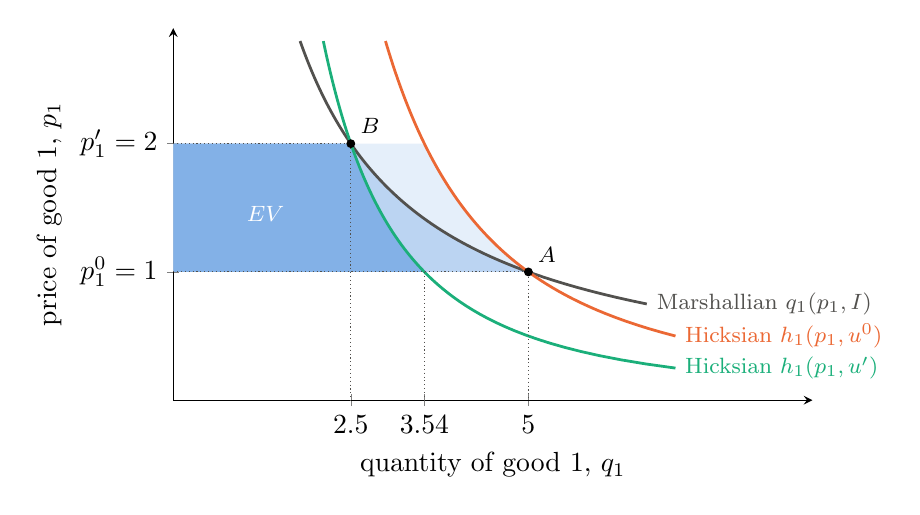
\begin{tikzpicture}
\begin{axis}[
  width=0.8\textwidth, height=0.52\textwidth,
  axis lines=left, xmin=0, xmax=9, ymin=0, ymax=2.9,
  xlabel={quantity of good 1, $q_1$}, ylabel={price of good 1, $p_1$},
  xtick={2.5,3.5355,5}, xticklabels={$2.5$,$3.54$,$5$},
  ytick={1,2}, yticklabels={$p_1^0 = 1$,$p_1' = 2$},
  every axis plot/.append style={line width=1pt},
  clip=false]
\addplot[draw=none, fill=c05p1blue!12, domain=1:2, samples=60, variable=\t]
  ({5/sqrt(\t)},{\t}) -- (axis cs:0,2) -- (axis cs:0,1) -- cycle;
\addplot[draw=none, fill=c05p1blue!32, domain=1:2, samples=60, variable=\t]
  ({5/\t},{\t}) -- (axis cs:0,2) -- (axis cs:0,1) -- cycle;
\addplot[draw=none, fill=c05p1blue!58, domain=1:2, samples=60, variable=\t]
  ({3.5355/sqrt(\t)},{\t}) -- (axis cs:0,2) -- (axis cs:0,1) -- cycle;
\addplot[c05p1gray, domain=0.75:2.8, samples=80, variable=\t] ({5/\t},{\t});
\addplot[c05p1orange, domain=0.5:2.8, samples=80, variable=\t] ({5/sqrt(\t)},{\t});
\addplot[c05p1aqua, domain=0.25:2.8, samples=80, variable=\t] ({3.5355/sqrt(\t)},{\t});
\node[anchor=west, font=\footnotesize, text=c05p1gray] at (axis cs:6.67,0.75) {Marshallian $q_1(p_1, I)$};
\node[anchor=west, font=\footnotesize, text=c05p1orange] at (axis cs:7.07,0.5) {Hicksian $h_1(p_1, u^0)$};
\node[anchor=west, font=\footnotesize, text=c05p1aqua] at (axis cs:7.07,0.25) {Hicksian $h_1(p_1, u')$};
\draw[densely dotted, c05p1gray] (axis cs:0,1) -- (axis cs:5,1) -- (axis cs:5,0);
\draw[densely dotted, c05p1gray] (axis cs:0,2) -- (axis cs:2.5,2) -- (axis cs:2.5,0);
\draw[densely dotted, c05p1gray] (axis cs:3.5355,1) -- (axis cs:3.5355,0);
\fill (axis cs:5,1) circle (1.6pt) node[above right, font=\footnotesize] {$A$};
\fill (axis cs:2.5,2) circle (1.6pt) node[above right, font=\footnotesize] {$B$};
\node[font=\footnotesize, text=white] at (axis cs:1.3,1.45) {$EV$};
\end{axis}
\end{tikzpicture}
\caption{Compensating variation, equivalent variation and Marshallian surplus for a rise in $p_1$ from 1 to 2
(\cref{ex:05-cobb-douglas}: $U = q_1^{\frac{1}{2}}q_2^{\frac{1}{2}}$, $p_2 = 1$, $I = 10$). The consumer
moves from $A$ to $B$ along the Marshallian demand. The Hicksian demand at the initial utility $u^0$ passes
through $A$, and the Hicksian demand at the final utility $u'$ passes through $B$. The darkest region is the
$EV$ (2.93). Adding the middle band gives the Marshallian surplus loss (3.47). Adding the lightest band gives
the $CV$ (4.14).}\label{fig:05-cv-area}
\end{figure}

\subsection{Flexible functional forms}\label{sec:05-flexible}

An empirical demand system must take a parametric form. We want a form general enough not to prejudge the
answers, yet tied to preferences so that it satisfies the restrictions above. The concept that formalizes
``general enough'' is flexibility.

\begin{definition}[Flexible functional form]\label{def:05-flexible}
A parametric expenditure function $e(p, u; \theta)$ is a \emph{flexible functional form} if it can match
any expenditure function to second order at any point \citep{Diewert1974}. Formally, let $(p^0, u^0)$ be any
point and let $\tilde e$ be any twice continuously differentiable expenditure function with the properties of
\cref{prop:05-e-properties}. Then there is a parameter value $\theta$ such that $e$ and $\tilde e$ have the
same value and the same first and second partial derivatives with respect to $(p, u)$ at $(p^0, u^0)$.
\end{definition}

A flexible expenditure function is a second-order approximation to any expenditure function at a point. By
Shephard's lemma its first price derivatives are the Hicksian demands, and its second price derivatives are
the Slutsky terms. The cross derivatives in $p$ and $u$ determine the income effects, because
$\frac{\partial h_i}{\partial u} = \frac{\partial q_i}{\partial I}\frac{\partial e}{\partial u}$. A flexible
expenditure function therefore generates demands whose levels and first derivatives in prices and income can
match those of any demand system at a point. In this sense it is a first-order approximation to demand.

The search for such forms has a long history, which \citet[p.~312]{DeatonMuellbauer1980a} summarize. The
\emph{linear expenditure system} of \citet{Stone1954} was the first system estimated from an explicit utility
function. Its additive utility function leaves only $2J - 1$ free parameters, too few for flexibility, and it
rules out inferior goods and Hicksian complements. The \emph{Rotterdam model} of \citet{Theil1965} and
\citet{Barten1969} approximates the demand functions themselves in differential form, with constant
coefficients on which the restrictions of theory are linear. The \emph{translog model} of
\citet{ChristensenJorgensonLau1975} takes a second-order approximation to the indirect utility function,
$\ln v = \alpha_0 + \sum_i\alpha_i\ln\frac{p_i}{I} + \frac{1}{2}\sum_i\sum_j b_{ij}\ln\frac{p_i}{I}\ln\frac{p_j}{I}$.
By Roy's identity its shares are ratios of linear functions of the log normalized prices, which makes
estimation nonlinear. The AIDS was designed to combine the virtues of these models. It starts from a class
of preferences that permits aggregation over consumers, and it yields shares that are nearly linear in the
parameters.

\section{The Almost Ideal Demand System}\label{sec:05-aids}

\citet{DeatonMuellbauer1980a} derive the AIDS from a specific expenditure function. We follow their
derivation step by step, then establish the restrictions, the elasticities, the flexibility of the system and
its Engel curves, and we close with its limits.

\subsection{The PIGLOG class}\label{sec:05-piglog}

\begin{definition}[PIGLOG preferences]\label{def:05-piglog}
Preferences belong to the \emph{price-independent generalized logarithmic} (PIGLOG) class if the expenditure
function can be written as
\begin{equation}\label{eq:05-piglog}
\ln e(p, u) = (1 - u)\ln a(p) + u\ln b(p),
\end{equation}
where $a(p)$ and $b(p)$ are positive, linearly homogeneous and concave functions of prices.
\end{definition}

Equation \eqref{eq:05-piglog} is equation (1) of \citet[p.~313]{DeatonMuellbauer1980a}, who write the
expenditure function as $c(u, p)$. With some exceptions that they discuss in their appendix, utility lies
between $0$ and $1$. At $u = 0$ expenditure equals $a(p)$, and at $u = 1$ it equals $b(p)$. The two
functions can therefore be regarded as the costs of \emph{subsistence} and of \emph{bliss}
\citep[p.~313]{DeatonMuellbauer1980a}. The class is due to \citet{Muellbauer1975,Muellbauer1976}, who showed
that these preferences permit aggregation over consumers. Market demands can then be represented as if they
were the decisions of one rational representative consumer, with a representative budget level that does not
depend on prices. \Cref{sec:05-aggregation} develops this property.

Two consequences of \eqref{eq:05-piglog} are useful at once. First, the expenditure function equals
$e = a(p)^{1-u}b(p)^u$, a weighted geometric mean of $a$ and $b$. The geometric mean is concave and
increasing in its arguments, so $e$ is concave in $p$ whenever $a$ and $b$ are concave and $0 \leq u \leq 1$.
\citet[p.~324]{DeatonMuellbauer1980a} note that this condition is sufficient for concavity but by no
means necessary. Second, Shephard's lemma in share form gives
\begin{equation}\label{eq:05-piglog-weights}
w_i = (1 - u)\frac{\partial\ln a(p)}{\partial\ln p_i} + u\frac{\partial\ln b(p)}{\partial\ln p_i} .
\end{equation}
Budget shares are weighted averages of the subsistence shares and the bliss shares, with weights given by
utility \citep[p.~324]{DeatonMuellbauer1980a}. Luxuries are the goods whose bliss share exceeds their
subsistence share. Inverting $\ln I = \ln a + u(\ln b - \ln a)$ gives
$u = \frac{\ln I - \ln a(p)}{\ln b(p) - \ln a(p)}$. Substituting into \eqref{eq:05-piglog-weights} shows that
every PIGLOG share is linear in $\ln I$, with intercept and slope that depend on prices:
\begin{equation}\label{eq:05-piglog-share}
w_i = \frac{\partial\ln a(p)}{\partial\ln p_i} + \frac{\partial\ln\frac{b(p)}{a(p)}}{\partial\ln p_i}\cdot
\frac{\ln I - \ln a(p)}{\ln\frac{b(p)}{a(p)}} .
\end{equation}

\subsection{The AIDS cost function}\label{sec:05-aids-cost}

\citet[p.~313]{DeatonMuellbauer1980a} choose specific forms for $a(p)$ and $b(p)$:
\begin{align}
\ln a(p) &= \alpha_0 + \sum_k\alpha_k\ln p_k + \frac{1}{2}\sum_k\sum_j\gamma^*_{kj}\ln p_k\ln p_j,
  \label{eq:05-aids-a}\\
\ln b(p) &= \ln a(p) + \beta_0\prod_k p_k^{\beta_k}. \label{eq:05-aids-b}
\end{align}
Substituting into \eqref{eq:05-piglog} gives the \emph{AIDS cost function}
\begin{equation}\label{eq:05-aids-cost}
\ln e(p, u) = \alpha_0 + \sum_k\alpha_k\ln p_k + \frac{1}{2}\sum_k\sum_j\gamma^*_{kj}\ln p_k\ln p_j
+ u\beta_0\prod_k p_k^{\beta_k},
\end{equation}
where $\alpha_0$, $\alpha_k$, $\beta_0$, $\beta_k$ and $\gamma^*_{kj}$ are parameters. The subsistence cost
$\ln a(p)$ is a translog function of prices, and the gap between bliss and subsistence, $\ln b - \ln a$, is a
Cobb-Douglas function of prices. According to \citet[p.~313]{DeatonMuellbauer1980a}, the choice is governed
partly by the need for flexibility, and mainly by the desirable properties of the demand functions it
generates. At unit prices and $u = 0$ expenditure is $e^{\alpha_0}$, so $e^{\alpha_0}$ is the outlay needed for
subsistence when all prices equal one.

\begin{proposition}[Homogeneity of the AIDS cost function]\label{prop:05-aids-homog}
Let $\gamma_{kj} = \frac{1}{2}(\gamma^*_{kj} + \gamma^*_{jk})$. The function \eqref{eq:05-aids-cost} is
homogeneous of degree one in $p$ for all $u$ if and only if
\begin{equation}\label{eq:05-aids-homog}
\sum_k\alpha_k = 1, \qquad \sum_j\gamma_{kj} = 0 \ \text{ for every } k, \qquad \sum_k\beta_k = 0 .
\end{equation}
In particular, the conditions $\sum_j\gamma^*_{kj} = \sum_k\gamma^*_{kj} = 0$ stated by
\citet[p.~313]{DeatonMuellbauer1980a}, together with $\sum_k\alpha_k = 1$ and $\sum_k\beta_k = 0$, are
sufficient.
\end{proposition}

\begin{proof}
The quadratic form depends on $\gamma^*$ only through its symmetric part, because for any vector $x$
\begin{equation*}
\sum_k\sum_j\gamma^*_{kj}x_kx_j = \sum_k\sum_j\gamma_{kj}x_kx_j .
\end{equation*}
Write
$\ell = \ln\lambda$ and $R_k = \sum_j\gamma_{kj}$. Replace $\ln p_k$ by $\ln p_k + \ell$ in
\eqref{eq:05-aids-cost} and subtract $\ln e(p, u) + \ell$. The linear part contributes
$\big(\sum_k\alpha_k - 1\big)\ell$. The quadratic part contributes
\begin{equation*}
\frac{1}{2}\sum_k\sum_j\gamma_{kj}\big[(\ln p_k + \ell)(\ln p_j + \ell) - \ln p_k\ln p_j\big]
= \ell\sum_k R_k\ln p_k + \frac{1}{2}\ell^2\sum_k R_k ,
\end{equation*}
where we used the symmetry of $\gamma$ to combine the two cross terms. The last term contributes
$u\beta_0\prod_k p_k^{\beta_k}\big(\lambda^{\sum_k\beta_k} - 1\big)$. Under \eqref{eq:05-aids-homog} every
contribution vanishes, which proves sufficiency. For necessity, the total must vanish for all $\lambda$, $p$
and $u$. At $u = 0$ and unit prices it equals $\big(\sum_k\alpha_k - 1\big)\ell + \frac{1}{2}\ell^2\sum_kR_k$,
so $\sum_k\alpha_k = 1$ and $\sum_kR_k = 0$. At $u = 0$ and arbitrary prices it then equals
$\ell\sum_kR_k\ln p_k$, so every $R_k = 0$. At $u > 0$ the remaining term forces
$\lambda^{\sum_k\beta_k} = 1$ for all $\lambda$, that is, $\sum_k\beta_k = 0$. The stated conditions on
$\gamma^*$ imply $R_k = \frac{1}{2}\big(\sum_j\gamma^*_{kj} + \sum_j\gamma^*_{jk}\big) = 0$.
\end{proof}

\begin{remark}[Two normalizations]\label{rem:05-aids-normalizations}
The expenditure function depends on $u$ and $\beta_0$ only through their product $u\beta_0$. Replacing $u$ by
$\frac{u}{c}$ and $\beta_0$ by $c\beta_0$ for any $c > 0$ changes nothing observable, because it only
rescales utility. Since utility is ordinal, we may set $\beta_0 = 1$, and we do so in numerical work. The
expenditure function increases in $u$ only if $\beta_0 > 0$. The second normalization concerns curvature in
utility. Because $\ln e$ is linear in $u$, the AIDS sets $\frac{\partial^2\ln e}{\partial u^2} = 0$
everywhere. \citet[p.~313]{DeatonMuellbauer1980a} point out that this costs no generality, because an
ordinal normalization of utility can always set this derivative to zero at a point.
\end{remark}

A parameter count shows that the AIDS cost function has just enough parameters to be flexible. Consider an
arbitrary expenditure function and a point $(p^0, u^0)$. Its value, its $J$ price derivatives and its
derivative in $u$ make $J + 2$ numbers. Its second derivatives add $\frac{J(J+1)}{2}$ distinct price terms,
$J$ cross terms in $p$ and $u$, and one term in $u$, for a total of $\frac{J(J+1)}{2} + 2J + 3$. Homogeneity of
degree one imposes Euler's equation on the value, on the first price derivatives and on the derivative in
$u$, which removes $J + 2$ of them. That leaves $\frac{(J+1)(J+2)}{2}$ free numbers. The AIDS has
$\alpha_0$, $J - 1$ free $\alpha_k$, $\frac{J(J-1)}{2}$ free $\gamma_{kj}$, $J - 1$ free $\beta_k$ and
$\beta_0$, which is $\frac{J(J+3)}{2}$ parameters. The difference is exactly one, the second derivative in
$u$, which the ordinal normalization of \cref{rem:05-aids-normalizations} absorbs. A count is necessary but
not sufficient for flexibility. \Cref{prop:05-flexible} proves the corresponding property for demands by
construction.

\subsection{Deriving the share equations}\label{sec:05-aids-shares}

We derive the budget shares in six steps.

\casehead{Step 1} Shephard's lemma in share form gives the shares. By \eqref{eq:05-shephard-share}, the budget share of good $i$
is the derivative of \eqref{eq:05-aids-cost} with respect to $\ln p_i$
\citep[eq.~5]{DeatonMuellbauer1980a}:
\begin{equation*}
w_i = \frac{\partial\ln e(p, u)}{\partial\ln p_i}.
\end{equation*}

\casehead{Step 2} We differentiate the translog part. The linear term contributes $\alpha_i$. In the quadratic term, $\ln p_i$
appears once as $\ln p_k$ (when $k = i$) and once as $\ln p_j$ (when $j = i$):
\begin{equation*}
\frac{\partial}{\partial\ln p_i}\Big[\frac{1}{2}\sum_k\sum_j\gamma^*_{kj}\ln p_k\ln p_j\Big]
= \frac{1}{2}\sum_j\gamma^*_{ij}\ln p_j + \frac{1}{2}\sum_k\gamma^*_{ki}\ln p_k
= \sum_j\gamma_{ij}\ln p_j ,
\end{equation*}
where
\begin{equation}\label{eq:05-gamma-sym}
\gamma_{ij} = \frac{1}{2}\big(\gamma^*_{ij} + \gamma^*_{ji}\big)
\end{equation}
is equation (7) of \citet{DeatonMuellbauer1980a}. The coefficients $\gamma_{ij}$ that enter the share
equations are symmetric by construction when the system is derived from the cost function.

\casehead{Step 3} We differentiate the Cobb-Douglas part. Write the product as an exponential and differentiate:
\begin{equation*}
\frac{\partial}{\partial\ln p_i}\prod_k p_k^{\beta_k} = \frac{\partial}{\partial\ln p_i}
\exp\Big(\sum_k\beta_k\ln p_k\Big) = \beta_i\prod_k p_k^{\beta_k}.
\end{equation*}

\casehead{Step 4} Collecting the three pieces gives the shares as functions of prices and
utility \citep[eq.~6]{DeatonMuellbauer1980a}:
\begin{equation}\label{eq:05-aids-hicks-share}
w_i(p, u) = \alpha_i + \sum_j\gamma_{ij}\ln p_j + \beta_iu\beta_0\prod_k p_k^{\beta_k} .
\end{equation}

\casehead{Step 5} We now solve for indirect utility. Define the \emph{translog price index}
\begin{equation}\label{eq:05-translog}
\ln\mathbf{P}(p) = \alpha_0 + \sum_k\alpha_k\ln p_k + \frac{1}{2}\sum_k\sum_j\gamma_{kj}\ln p_k\ln p_j ,
\end{equation}
which is equation (9) of \citet{DeatonMuellbauer1980a}. By the first step of the proof of
\cref{prop:05-aids-homog}, $\ln\mathbf{P}(p) = \ln a(p)$, so the price index is the subsistence cost. Write
\begin{equation}\label{eq:05-aids-B}
B(p) = \beta_0\prod_k p_k^{\beta_k} = \ln b(p) - \ln a(p)
\end{equation}
for the Cobb-Douglas part of the cost function. The cost function becomes
$\ln e(p, u) = \ln\mathbf{P}(p) + u\,B(p)$. A utility-maximizing consumer spends $e(p, u) = I$. Solving for
$u$ gives the indirect utility function
\begin{equation}\label{eq:05-aids-v}
v(p, I) = \frac{\ln I - \ln\mathbf{P}(p)}{B(p)} .
\end{equation}

\casehead{Step 6} We obtain the Marshallian shares. At $u = v(p, I)$, the last term of
\eqref{eq:05-aids-hicks-share} equals $\beta_iuB(p) = \beta_i\big(\ln I - \ln\mathbf{P}\big)$. The AIDS demand functions in budget share form are therefore
\begin{equation}\label{eq:05-aids-share}
w_i = \alpha_i + \sum_{j=1}^J\gamma_{ij}\ln p_j + \beta_i\ln\frac{I}{\mathbf{P}} ,
\qquad i = 1, \dots, J,
\end{equation}
which is equation (8) of \citet{DeatonMuellbauer1980a}.

Roy's identity gives the same result from \eqref{eq:05-aids-v}, which is a useful check. By Step 3,
$\frac{\partial B}{\partial\ln p_i} = \beta_iB$. Then $\frac{\partial v}{\partial\ln I} = \frac{1}{B}$ and
\begin{equation*}
\frac{\partial v}{\partial\ln p_i} = -\frac{1}{B}\frac{\partial\ln\mathbf{P}}{\partial\ln p_i}
- \frac{\ln I - \ln\mathbf{P}}{B}\beta_i .
\end{equation*}
The share form of \eqref{eq:05-roy} gives
$w_i = \frac{\partial\ln\mathbf{P}}{\partial\ln p_i} + \beta_i\ln\frac{I}{\mathbf{P}}$. Step 2 applied to
\eqref{eq:05-translog} gives $\frac{\partial\ln\mathbf{P}}{\partial\ln p_i} = \alpha_i + \sum_j\gamma_{ij}\ln
p_j$, which reproduces \eqref{eq:05-aids-share}.

The parameters have simple interpretations \citep[p.~314]{DeatonMuellbauer1980a}. When relative prices and
real expenditure $\frac{I}{\mathbf{P}}$ do not change, the budget shares are constant. This is the natural
starting point for predictions with the model. Changes in relative prices work through the $\gamma_{ij}$.
Each $\gamma_{ij}$ is 100 times the change in the budget share of good $i$ caused by a one percent rise in
$p_j$ with $\frac{I}{\mathbf{P}}$ held constant. The factor 100 appears because such a rise increases
$\ln p_j$ by about $0.01$.
Changes in real expenditure work through the $\beta_i$, which sum to zero. They are positive for luxuries and
negative for necessities, as \eqref{eq:05-eta} below confirms. Real expenditure is measured relative to the
subsistence cost $\mathbf{P}(p) = a(p)$. The price index depends on the parameters $\alpha_0$, $\alpha_k$ and
$\gamma_{kj}$, which makes the system nonlinear in its parameters. \Cref{sec:05-estimation} discusses how to
estimate it, including the common approximation of $\mathbf{P}$ by a price index computed from data.

\begin{remark}[From Engel curves to the AIDS]\label{rem:05-working-leser}
\citet[\S 3.4, pp.~75--77]{DeatonMuellbauer1980b} reach the AIDS from the data side. Budget studies
support the \emph{Working-Leser} Engel curve, in which the budget share is linear in the log budget, $w_i
= \tilde\alpha_i + \tilde\beta_i\ln I$ at fixed prices (their eq.~4.1, \citealp{Working1943,Leser1963}). To
use it on time series, the coefficients must become functions of prices in a way consistent with
preferences. Any expenditure function of the form
\begin{equation*}
  \ln e(p, u) = A(p) + u\,B(p)
\end{equation*}
does this (their eq.~4.2). Write $A_i = \frac{\partial A}{\partial\ln p_i}$ and $B_i = \frac{\partial
B}{\partial\ln p_i}$. Shephard's lemma in share form gives $w_i = A_i(p) + u\,B_i(p)$. Inverting $\ln I =
A(p) + uB(p)$ gives $u = \frac{\ln I - A(p)}{B(p)}$. Substituting,
\begin{equation*}
  w_i = \Bigl[A_i(p) - \frac{B_i(p)}{B(p)}A(p)\Bigr] + \frac{B_i(p)}{B(p)}\ln I ,
\end{equation*}
which has the Working-Leser form at every price vector. The AIDS chooses $A(p)$ translog and $B(p) =
\beta_0\prod_k p_k^{\beta_k}$, as in their eqs.~(4.3)--(4.4). Then $\frac{B_i}{B} = \beta_i$ is constant,
$A_i = \alpha_i + \sum_j\gamma_{ij}\ln p_j$, and the display becomes \eqref{eq:05-aids-share}. The book's
$A(p)$ is the article's $\ln a(p)$, and its $B(p)$ is the article's $\ln b(p) - \ln a(p)$, which is
\eqref{eq:05-aids-B}. The two derivations therefore describe the same model. The book also states the
negativity condition with a matrix $C$, its eq.~(4.12), which is our $K$ of \eqref{eq:05-K}. It stresses
that the matrix $[\gamma_{ij}]$ itself need not be negative semidefinite (p.~76).
\end{remark}

\subsection{Restrictions from consumer theory}\label{sec:05-aids-restrictions}

Suppose we take the share equations \eqref{eq:05-aids-share} with the index \eqref{eq:05-translog} as a
maintained hypothesis, with unrestricted coefficients $\gamma_{ij}$, as
\citet[p.~316]{DeatonMuellbauer1980a} do. The next proposition states which linear restrictions make the
system consistent with demand theory.

\begin{proposition}[Adding up, homogeneity and symmetry]\label{prop:05-restrictions}
Consider \eqref{eq:05-aids-share} and \eqref{eq:05-translog}.
\begin{enumerate}[label=(\roman*)]
\item The shares sum to one at all $(p, I)$ if and only if
  \begin{equation}\label{eq:05-adding-up}
  \sum_i\alpha_i = 1, \qquad \sum_i\gamma_{ij} = 0 \ \text{ for every } j, \qquad \sum_i\beta_i = 0 .
  \end{equation}
\item Given \eqref{eq:05-adding-up}, demands are homogeneous of degree zero in $(p, I)$ if and only if
  \begin{equation}\label{eq:05-homogeneity}
  \sum_j\gamma_{ij} = 0 \ \text{ for every } i .
  \end{equation}
\item Given \eqref{eq:05-adding-up} and \eqref{eq:05-homogeneity}, the Slutsky matrix is symmetric at all
  $(p, I)$ if and only if
  \begin{equation}\label{eq:05-symmetry}
  \gamma_{ij} = \gamma_{ji} \ \text{ for all } i, j .
  \end{equation}
\end{enumerate}
\end{proposition}

\begin{proof}
(i) Sum \eqref{eq:05-aids-share} over $i$:
\begin{equation*}
\sum_iw_i = \sum_i\alpha_i + \sum_j\Big(\sum_i\gamma_{ij}\Big)\ln p_j + \Big(\sum_i\beta_i\Big)\ln\frac{I}{\mathbf{P}} .
\end{equation*}
Given $p$, the term $\ln I$ varies freely, so the sum equals one for all $I$ only if $\sum_i\beta_i = 0$.
Then $\sum_j\big(\sum_i\gamma_{ij}\big)\ln p_j = 1 - \sum_i\alpha_i$ for all log prices, which requires every
coefficient to vanish and the constant to be zero. The converse is immediate.

(ii) Write $\ell = \ln\lambda$ and $R_i = \sum_j\gamma_{ij}$. Because \eqref{eq:05-adding-up} makes the
column sums of $\gamma$ zero and $\sum_k\alpha_k = 1$, the computation in the proof of
\cref{prop:05-aids-homog} gives
$\ln\mathbf{P}(\lambda p) = \ln\mathbf{P}(p) + \ell + \frac{1}{2}\ell\sum_kR_k\ln p_k + \frac{1}{2}\ell^2\sum_kR_k$.
Hence
\begin{equation*}
w_i(\lambda p, \lambda I) - w_i(p, I) = \ell R_i - \beta_i\Big[\frac{1}{2}\ell\sum_kR_k\ln p_k +
\frac{1}{2}\ell^2\sum_kR_k\Big].
\end{equation*}
If every $R_k = 0$, the difference vanishes. Conversely, at unit prices the difference is
$\ell R_i - \frac{1}{2}\beta_i\ell^2\sum_kR_k$, and it vanishes for all $\lambda$ only if $R_i = 0$.

(iii) Let $\gamma^s_{jk} = \frac{1}{2}(\gamma_{jk} + \gamma_{kj})$ and $r = \ln\frac{I}{\mathbf{P}}$. Then
$\frac{\partial w_i}{\partial\ln I} = \beta_i$, $\frac{\partial\ln\mathbf{P}}{\partial\ln p_j} = \alpha_j +
\sum_k\gamma^s_{jk}\ln p_k$, and
$\frac{\partial w_i}{\partial\ln p_j} = \gamma_{ij} - \beta_i\frac{\partial\ln\mathbf{P}}{\partial\ln p_j}$.
Using $w_j = \alpha_j + \sum_k\gamma_{jk}\ln p_k + \beta_jr$, the first two terms of \eqref{eq:05-K-general}
are
\begin{equation*}
\frac{\partial w_i}{\partial\ln p_j} + w_j\frac{\partial w_i}{\partial\ln I}
= \gamma_{ij} + \beta_i\beta_jr + \beta_i\sum_k\big(\gamma_{jk} - \gamma^s_{jk}\big)\ln p_k .
\end{equation*}
The remaining terms of \eqref{eq:05-K-general}, $w_iw_j - \indic(i=j)w_i$, are symmetric in $(i, j)$. Under
\eqref{eq:05-symmetry} the last sum vanishes and $k_{ij} = \gamma_{ij} + \beta_i\beta_jr + w_iw_j -
\indic(i=j)w_i$ is symmetric, so $S_{ij} = \frac{I\,k_{ij}}{p_ip_j}$ is symmetric. Conversely, at unit prices the
expression reduces to $\gamma_{ij} + \beta_i\beta_jr$, which is symmetric only if $\gamma_{ij} = \gamma_{ji}$.
\end{proof}

These are equations (10) to (12) of \citet[p.~314]{DeatonMuellbauer1980a}. All three sets are linear in the
parameters and do not involve the data, so they can be imposed globally by standard methods. They differ in
how they can be tested \citep[p.~316]{DeatonMuellbauer1980a}. Adding up cannot be tested on share data,
because observed shares add up to one by construction and the estimated parameters satisfy
\eqref{eq:05-adding-up} automatically. Homogeneity involves the parameters of a single equation and can be
tested equation by equation. Symmetry links the parameters of two equations and can only be tested in a
system. \Cref{sec:05-testing} carries out these tests.

\subsection{Negativity}\label{sec:05-negativity}

Concavity of the expenditure function is the fourth restriction, and it is of a different kind.

\begin{proposition}[Negativity of the AIDS]\label{prop:05-negativity}
Under \eqref{eq:05-adding-up}, \eqref{eq:05-homogeneity} and \eqref{eq:05-symmetry}, the Slutsky terms of the
AIDS satisfy
\begin{equation}\label{eq:05-hicks-deriv}
\frac{\partial h_i(p, u)}{\partial p_j} = \frac{e(p, u)}{p_ip_j}\Big[\frac{\partial w_i(p,u)}{\partial\ln p_j}
+ w_iw_j - \indic(i=j)w_i\Big],
\end{equation}
where $w_i(p, u)$ is the Hicksian share \eqref{eq:05-aids-hicks-share}. The matrix $K = [k_{ij}]$ with
$k_{ij} = \frac{p_ip_jS_{ij}}{I}$ equals
\begin{equation}\label{eq:05-K}
k_{ij} = \gamma_{ij} + \beta_i\beta_j\ln\frac{I}{\mathbf{P}} - \indic(i=j)w_i + w_iw_j ,
\end{equation}
and its eigenvalues have the same signs as those of $S$. The AIDS satisfies negativity at $(p, I)$ if and
only if $K$ is negative semidefinite there.
\end{proposition}

\begin{proof}
By Shephard's lemma and \eqref{eq:05-shephard-share}, $h_i = \frac{w_i(p,u)e(p,u)}{p_i}$. Differentiate with
respect to $p_j$ by the product rule:
\begin{equation*}
\frac{\partial h_i}{\partial p_j} = \frac{e}{p_i}\frac{\partial w_i}{\partial p_j} + \frac{w_i}{p_i}
\frac{\partial e}{\partial p_j} - \indic(i=j)\frac{w_ie}{p_i^2} .
\end{equation*}
Substitute $\frac{\partial w_i}{\partial p_j} = \frac{1}{p_j}\frac{\partial w_i}{\partial\ln p_j}$ and
$\frac{\partial e}{\partial p_j} = h_j = \frac{w_je}{p_j}$, and factor out $\frac{e}{p_ip_j}$ to obtain
\eqref{eq:05-hicks-deriv}. For the AIDS, differentiating \eqref{eq:05-aids-hicks-share} and using Step 3 gives
\begin{equation*}
\frac{\partial w_i(p, u)}{\partial\ln p_j} = \gamma_{ij} + \beta_i\beta_ju\beta_0\prod_kp_k^{\beta_k}
= \gamma_{ij} + \beta_i\beta_j\ln\frac{I}{\mathbf{P}} ,
\end{equation*}
where the second equality evaluates at $u = v(p, I)$. Multiplying \eqref{eq:05-hicks-deriv} by
$\frac{p_ip_j}{I}$ with $e = I$ gives \eqref{eq:05-K}. Finally, $K = \frac{1}{I}DSD$ with
$D = \diag(p_1, \dots, p_J)$ nonsingular. By Sylvester's law of inertia, congruent symmetric matrices have
the same numbers of positive, negative and zero eigenvalues.
\end{proof}

Equation \eqref{eq:05-K} is equation (14) of \citet[p.~316]{DeatonMuellbauer1980a}. It agrees with the
general formula \eqref{eq:05-K-general}, as the proof of \cref{prop:05-restrictions} showed. Three features
matter in practice. First, the rows of $K$ sum to zero:
$\sum_jk_{ij} = \sum_j\gamma_{ij} + \beta_i\ln\frac{I}{\mathbf{P}}\sum_j\beta_j - w_i + w_i\sum_jw_j = 0$. This is the share-form
counterpart of $Sp = 0$. One eigenvalue of $K$ is therefore identically zero, and negativity requires the
other $J - 1$ eigenvalues to be nonpositive. Second, $K$ depends on the data point through the shares and
through $\ln\frac{I}{\mathbf{P}}$. As with other flexible forms, no restriction on the parameters alone can
guarantee negativity \citep[p.~316]{DeatonMuellbauer1980a}. Negativity can be checked observation by
observation by computing the eigenvalues of $K$ at the estimates. It can also be imposed at a single point. We
write $K$ at that point as $-LL^\T$, with $L$ lower triangular, and estimate the elements of $L$ in place of
the $\gamma_{ij}$ \citep{Lau1978,Moschini1999}. Third, part (f) of \cref{prop:05-elast-identities} gives
$\varepsilon^h_{ij} = \frac{k_{ij}}{w_i}$, so that for $i \neq j$
\begin{equation}\label{eq:05-gamma-sign}
\varepsilon^h_{ij} = \frac{\gamma_{ij} + \beta_i\beta_j\ln\frac{I}{\mathbf{P}}}{w_i} + w_j .
\end{equation}
When $\beta_i\beta_j\ln\frac{I}{\mathbf{P}} + w_iw_j$ is small relative to $\gamma_{ij}$, the coefficient
$\gamma_{ij}$ has the sign of the compensated cross-price elasticity. This is the approximation that
\citet[p.~315]{DeatonMuellbauer1980a} invoke when they suggest using prior beliefs about substitutes and
complements to restrict individual $\gamma_{ij}$.

\subsection{Elasticities}\label{sec:05-aids-elasticities}

The elasticities follow from three derivatives of the Marshallian shares. Throughout, write
$r = \ln\frac{I}{\mathbf{P}}$ and impose \eqref{eq:05-adding-up}, \eqref{eq:05-homogeneity} and
\eqref{eq:05-symmetry}. The derivative with respect to log income is
\begin{equation}\label{eq:05-dw-dI}
\frac{\partial w_i}{\partial\ln I} = \beta_i .
\end{equation}
Differentiating the translog index as in Step 2 and using the share equation for good $j$ gives
\begin{equation}\label{eq:05-dlnP}
\frac{\partial\ln\mathbf{P}}{\partial\ln p_j} = \alpha_j + \sum_k\gamma_{jk}\ln p_k = w_j - \beta_jr .
\end{equation}
The derivative with respect to a log price therefore has two equivalent forms:
\begin{equation}\label{eq:05-dw-dp}
\frac{\partial w_i}{\partial\ln p_j} = \gamma_{ij} - \beta_i\Big(\alpha_j + \sum_k\gamma_{jk}\ln p_k\Big)
= \gamma_{ij} - \beta_i\big(w_j - \beta_jr\big).
\end{equation}

To convert share derivatives into elasticities, write $q_i = \frac{w_iI}{p_i}$, so that
$\ln q_i = \ln w_i + \ln I - \ln p_i$. Differentiating with respect to $\ln I$ gives the expenditure
elasticity
\begin{equation}\label{eq:05-eta}
\eta_i = 1 + \frac{1}{w_i}\frac{\partial w_i}{\partial\ln I} = 1 + \frac{\beta_i}{w_i} .
\end{equation}
A good is a luxury ($\eta_i > 1$) if and only if $\beta_i > 0$, and a necessity if and only if
$\beta_i < 0$. Differentiating with respect to $\ln p_j$ gives the Marshallian price elasticity
\begin{equation}\label{eq:05-elast-marshall}
\varepsilon_{ij} = -\indic(i=j) + \frac{1}{w_i}\frac{\partial w_i}{\partial\ln p_j}
= -\indic(i=j) + \frac{\gamma_{ij} - \beta_i\big(w_j - \beta_j\ln\frac{I}{\mathbf{P}}\big)}{w_i} .
\end{equation}
The Slutsky equation of \cref{prop:05-elast-identities}(a) gives the Hicksian elasticity. Adding
$\eta_iw_j = w_j + \frac{\beta_iw_j}{w_i}$ to \eqref{eq:05-elast-marshall}, the terms in $\beta_iw_j$ cancel:
\begin{equation}\label{eq:05-elast-hicks}
\varepsilon^h_{ij} = \varepsilon_{ij} + \eta_iw_j
= -\indic(i=j) + w_j + \frac{\gamma_{ij} + \beta_i\beta_j\ln\frac{I}{\mathbf{P}}}{w_i} .
\end{equation}
This agrees with $\varepsilon^h_{ij} = \frac{k_{ij}}{w_i}$ from \eqref{eq:05-K}. Note that
\eqref{eq:05-elast-marshall} uses the derivative of the exact index \eqref{eq:05-dlnP}. Approximating that
derivative by $w_j$, as is common when $\mathbf{P}$ is replaced by a data index, changes the formula. We
return to this point in \cref{sec:05-stone}.

The elasticities satisfy the identities of \cref{prop:05-elast-identities} under the restrictions. Engel
aggregation holds because $\sum_iw_i\eta_i = \sum_iw_i + \sum_i\beta_i = 1$. Cournot aggregation holds
because
\begin{equation*}
\sum_iw_i\varepsilon_{ij} = -w_j + \sum_i\gamma_{ij} - \big(w_j - \beta_jr\big)\sum_i\beta_i = -w_j ,
\end{equation*}
using the adding-up restrictions on $\gamma$ and $\beta$. Homogeneity holds because
\begin{equation*}
\sum_j\varepsilon_{ij} + \eta_i = -1 + \frac{1}{w_i}\Big[\sum_j\gamma_{ij} - \beta_i\sum_j\alpha_j -
\beta_i\sum_k\Big(\sum_j\gamma_{jk}\Big)\ln p_k\Big] + 1 + \frac{\beta_i}{w_i} = 0 ,
\end{equation*}
where $\sum_j\gamma_{ij} = 0$ by homogeneity, and $\sum_j\alpha_j = 1$ and $\sum_j\gamma_{jk} = 0$ by adding
up. Symmetry holds because $w_i\varepsilon^h_{ij} = k_{ij}$ and $K$ is symmetric.

\begin{example}[The running example]\label{ex:05-running}
We use one numerical AIDS throughout the chapter. There are three goods, with $\alpha_0 = 0$,
$\alpha = (0.5, 0.3, 0.2)$, $\beta = (-0.10, 0.04, 0.06)$ and
\begin{equation*}
\Gamma = [\gamma_{ij}] = \begin{pmatrix} -0.20 & 0.12 & 0.08\\ 0.12 & -0.22 & 0.10\\ 0.08 & 0.10 & -0.18
\end{pmatrix}.
\end{equation*}
The parameters satisfy adding up, homogeneity and symmetry, since $\sum_i\alpha_i = 1$,
$\sum_i\beta_i = 0$, and $\Gamma$ is symmetric with zero row and column sums. Evaluate the system at
$p = (1, 1, 1)$ and $\ln I = 1$. All log prices are zero, so $\ln\mathbf{P} = \alpha_0 = 0$ and
$\ln\frac{I}{\mathbf{P}} = 1$. The shares are $w_i = \alpha_i + \beta_i$, that is,
$w = (0.40, 0.34, 0.26)$. Good 1 is a necessity, with $\eta_1 = 1 - \frac{0.10}{0.40} = 0.75$, and goods 2
and 3 are luxuries. For the own-price elasticity of good 1, \eqref{eq:05-elast-marshall} gives
\begin{equation*}
\varepsilon_{11} = -1 + \frac{-0.20 - (-0.10)\big(0.40 - (-0.10)(1)\big)}{0.40} = -1 + \frac{-0.15}{0.40}
= -1.375 ,
\end{equation*}
and the Hicksian elasticity is $\varepsilon^h_{11} = -1.375 + 0.75 \times 0.40 = -1.075$. The diagonal
element of $K$ is $k_{11} = -0.20 + 0.01 - 0.40 + 0.16 = -0.43$, and indeed
$\frac{k_{11}}{w_1} = -1.075$. \Cref{tab:05-running-example} reports the full matrices, computed with the
script \texttt{figures/ch05/src/aids\_example.py}. The identities hold to rounding. For the first column,
Cournot aggregation gives $0.40(-1.375) + 0.34(0.294) + 0.26(0.192) = -0.40 = -w_1$. For the first row,
homogeneity gives $-1.375 + 0.375 + 0.250 + 0.750 = 0$. Symmetry gives
$w_1\varepsilon^h_{12} = 0.40 \times 0.630 = 0.252 = 0.34 \times 0.741 = w_2\varepsilon^h_{21}$. The nonzero
eigenvalues of $K$ are $-0.689$ and $-0.552$, so the cost function is concave at this point.
\end{example}

\begin{table}[htbp]
\centering
\caption{The running example at $p = (1, 1, 1)$ and $\ln I = 1$}\label{tab:05-running-example}
\small
\begin{tabular}{c *{7}{S[table-format=-1.3]}}
\toprule
\multicolumn{8}{l}{\textit{A. Parameters, budget shares and expenditure elasticities} ($\alpha_0 = 0$)} \\
\midrule
Good $i$ & {$\alpha_i$} & {$\beta_i$} & {$\gamma_{i1}$} & {$\gamma_{i2}$} & {$\gamma_{i3}$} & {$w_i$} & {$\eta_i$} \\
\midrule
1 & 0.50 & -0.10 & -0.20 & 0.12 & 0.08 & 0.400 & 0.750 \\
2 & 0.30 & 0.04 & 0.12 & -0.22 & 0.10 & 0.340 & 1.118 \\
3 & 0.20 & 0.06 & 0.08 & 0.10 & -0.18 & 0.260 & 1.231 \\
\bottomrule
\end{tabular}

\medskip
\begin{tabular}{c *{9}{S[table-format=-1.3]}}
\toprule
\multicolumn{10}{l}{\textit{B. Price elasticities and the negativity matrix} (row $i$, price $j$)} \\
\midrule
 & \multicolumn{3}{c}{Marshallian $\varepsilon_{ij}$} & \multicolumn{3}{c}{Hicksian $\varepsilon^h_{ij}$}
 & \multicolumn{3}{c}{$k_{ij}$, equation \eqref{eq:05-K}} \\
\cmidrule(lr){2-4}\cmidrule(lr){5-7}\cmidrule(lr){8-10}
Good $i$ & {$j = 1$} & {$j = 2$} & {$j = 3$} & {$j = 1$} & {$j = 2$} & {$j = 3$} & {$j = 1$} & {$j = 2$}
 & {$j = 3$} \\
\midrule
1 & -1.375 & 0.375 & 0.250 & -1.075 & 0.630 & 0.445 & -0.430 & 0.252 & 0.178 \\
2 & 0.294 & -1.682 & 0.271 & 0.741 & -1.302 & 0.561 & 0.252 & -0.443 & 0.191 \\
3 & 0.192 & 0.315 & -1.738 & 0.685 & 0.734 & -1.418 & 0.178 & 0.191 & -0.369 \\
\midrule
\multicolumn{7}{l}{Eigenvalues of $K$} & -0.689 & -0.552 & 0.000 \\
\bottomrule
\end{tabular}
\par\smallskip
\begin{minipage}{0.92\textwidth}\footnotesize\raggedright
Notes: Elasticities are signed and computed from \eqref{eq:05-eta}, \eqref{eq:05-elast-marshall} and
\eqref{eq:05-elast-hicks}. The script \texttt{figures/ch05/src/aids\_example.py} also checks every analytic
elasticity against numerical derivatives of the demand functions, with a maximum discrepancy below $10^{-9}$.
\end{minipage}
\end{table}

\subsection{Flexibility*}\label{sec:05-aids-flexibility}

\citet[p.~315]{DeatonMuellbauer1980a} claim that the AIDS demand functions are first-order approximations to
any demand system, whether or not that system comes from utility maximization. We make the claim precise and
prove it by construction. A preliminary fact lets us work at unit prices.

\begin{lemma}[Units of measurement]\label{lem:05-units}
Let $\Gamma$ be symmetric, and measure good $k$ in new units, so that $\ln p_k = \ln\tilde p_k + c_k$ for
constants $c_k$. The AIDS in the new prices has the same $\gamma_{ij}$ and $\beta_i$, and the parameters
\begin{equation*}
\tilde\alpha_k = \alpha_k + \sum_j\gamma_{kj}c_j, \qquad
\tilde\alpha_0 = \alpha_0 + \sum_k\alpha_kc_k + \frac{1}{2}\sum_k\sum_j\gamma_{kj}c_kc_j .
\end{equation*}
These parameters satisfy \eqref{eq:05-adding-up}, \eqref{eq:05-homogeneity} and \eqref{eq:05-symmetry}
whenever the original ones do.
\end{lemma}

\begin{proof}
Substitute $\ln p_k = \ln\tilde p_k + c_k$ into \eqref{eq:05-translog} and expand the quadratic term, using
the symmetry of $\Gamma$ to combine the two cross terms:
\begin{equation*}
\ln\mathbf{P} = \Big[\alpha_0 + \sum_k\alpha_kc_k + \frac{1}{2}\sum_k\sum_j\gamma_{kj}c_kc_j\Big]
+ \sum_k\Big(\alpha_k + \sum_j\gamma_{kj}c_j\Big)\ln\tilde p_k
+ \frac{1}{2}\sum_k\sum_j\gamma_{kj}\ln\tilde p_k\ln\tilde p_j .
\end{equation*}
This is the translog index in the new prices with parameters $\tilde\alpha_0$ and $\tilde\alpha_k$. In the
share equation, $\alpha_i + \sum_j\gamma_{ij}\ln p_j = \tilde\alpha_i + \sum_j\gamma_{ij}\ln\tilde p_j$, and
income is unaffected. Hence every share is the same function of the data in either set of units. Finally,
$\sum_k\tilde\alpha_k = \sum_k\alpha_k + \sum_jc_j\sum_k\gamma_{kj} = 1$ under adding up, and $\Gamma$ is
unchanged.
\end{proof}

Fitted shares and elasticities therefore do not depend on the units in which goods are measured. Given any
point $(p^0, I^0)$, we can choose units so that $p^0 = (1, \dots, 1)$. We state the flexibility result at such
a point.

\begin{proposition}[First-order flexibility]\label{prop:05-flexible}
Fix a point $(p^0, I^0)$ with $p^0 = (1, \dots, 1)$. Let $w^0$ be any vector of positive budget shares that sum
to one, let $b_i$ be any numbers with $\sum_ib_i = 0$, and let $c_{ij}$ be any numbers with
$\sum_ic_{ij} = 0$ for every $j$.
\begin{enumerate}[label=(\roman*)]
\item There are AIDS parameters satisfying \eqref{eq:05-adding-up} such that, at $(p^0, I^0)$,
  $w_i = w^0_i$, $\frac{\partial w_i}{\partial\ln I} = b_i$ and $\frac{\partial w_i}{\partial\ln p_j} = c_{ij}$.
\item If in addition $\sum_jc_{ij} + b_i = 0$ for every $i$ (homogeneity) and $c_{ij} + b_iw^0_j$ is
  symmetric in $(i, j)$ (Slutsky symmetry), the parameters also satisfy \eqref{eq:05-homogeneity} and
  \eqref{eq:05-symmetry}.
\end{enumerate}
\end{proposition}

\begin{proof}
At unit prices all log prices are zero, so $\ln\mathbf{P}(p^0) = \alpha_0$ and
$\frac{\partial\ln\mathbf{P}}{\partial\ln p_j} = \alpha_j$ there, whether or not $\Gamma$ is symmetric. Choose
any real number $r^0$, which will be the value of $\ln\frac{I^0}{\mathbf{P}(p^0)}$. Set
\begin{equation*}
\beta_i = b_i, \qquad \alpha_j = w^0_j - b_jr^0, \qquad \gamma_{ij} = c_{ij} + b_i\alpha_j
= c_{ij} + b_iw^0_j - b_ib_jr^0, \qquad \alpha_0 = \ln I^0 - r^0 .
\end{equation*}
At $(p^0, I^0)$, the share of good $i$ is $\alpha_i + \beta_ir^0 = w^0_i$ and its income derivative is
$\beta_i = b_i$. Its price derivative is
$\gamma_{ij} - \beta_i\frac{\partial\ln\mathbf{P}}{\partial\ln p_j} = \gamma_{ij} - b_i\alpha_j = c_{ij}$.

For the restrictions in (i), $\sum_i\beta_i = \sum_ib_i = 0$,
$\sum_i\gamma_{ij} = \sum_ic_{ij} + \alpha_j\sum_ib_i = 0$, and
$\sum_j\alpha_j = \sum_jw^0_j - r^0\sum_jb_j = 1$. For (ii),
$\sum_j\gamma_{ij} = \sum_jc_{ij} + b_i\sum_jw^0_j - b_ir^0\sum_jb_j = \sum_jc_{ij} + b_i = 0$. The term
$b_ib_jr^0$ is symmetric, so $\gamma_{ij}$ is symmetric whenever $c_{ij} + b_iw^0_j$ is.
\end{proof}

The conditions on $(w^0, b, c)$ are exactly the restrictions that any demand system consistent with utility
maximization satisfies at a point. Adding up implies $\sum_iw_i = 1$, $\sum_ib_i = 0$ and $\sum_ic_{ij} = 0$.
Homogeneity of degree zero implies $\sum_jc_{ij} + b_i = 0$. By \eqref{eq:05-K-general}, Slutsky symmetry is
the symmetry of $c_{ij} + b_iw_j$, since the other terms of $k_{ij}$ are symmetric. Part (ii) therefore says
that the restricted AIDS can match the shares and the first derivatives of any utility-consistent demand
system at a point. Part (i) says that the AIDS without homogeneity and symmetry can match any demand system,
derived from theory or not. This second property matters for testing. Tests of homogeneity and symmetry are
then ``set within a maintained hypothesis which makes sense and would be widely accepted in its own right''
\citep[p.~315]{DeatonMuellbauer1980a}. The construction also shows that one parameter, $r^0$ or equivalently
$\alpha_0$, is left free. This foreshadows the difficulty of identifying $\alpha_0$ in practice
(\cref{sec:05-estimation}).

The count behind the proposition is worth stating. A utility-consistent demand system has $J - 1$ free
shares, $J - 1$ free income derivatives and $\frac{J(J-1)}{2}$ free Slutsky terms at a point. The restricted
AIDS has $J - 1$ free $\alpha_i$, $J - 1$ free $\beta_i$ and $\frac{J(J-1)}{2}$ free $\gamma_{ij}$. The two
counts coincide, so the theoretical restrictions remove as many free derivatives as free parameters.

\subsection{Engel curves and rank}\label{sec:05-engel}

An \emph{Engel curve} gives the budget share, or the expenditure, on a good as a function of total
expenditure at fixed prices. For the AIDS, collect the price terms in
$\zeta_i(p) = \alpha_i + \sum_j\gamma_{ij}\ln p_j - \beta_i\ln\mathbf{P}(p)$. Then
\begin{equation}\label{eq:05-engel}
w_i = \zeta_i(p) + \beta_i\ln I, \qquad p_iq_i = \zeta_i(p)\,I + \beta_i\,I\ln I .
\end{equation}
\citet[p.~317]{DeatonMuellbauer1980a} give the expenditure form in their discussion of budget studies.
Expenditure on good $i$ is
linear in $I$ only when $\beta_i = 0$. Its second derivative is $\frac{\beta_i}{I}$, so spending is convex in
income for luxuries and concave for necessities. The share form is the Engel curve of \citet{Working1943}.
\citet{Leser1963} recommended it as an excellent fit to cross-section data in a wide range of circumstances
\citep[p.~317]{DeatonMuellbauer1980a}. Before the AIDS, aggregation in time-series models
seemed to require linear Engel curves, while cross-section studies typically found them nonlinear. The AIDS
reconciles the two, because it aggregates with Engel curves of the Working-Leser form.

The flexibility of Engel curves is measured by the rank of the demand system.

\begin{definition}[Rank]\label{def:05-rank}
The \emph{rank} of a demand system is the largest dimension, over price vectors $p$, of the space of functions
of income spanned by its Engel curves $w_1(p, \cdot), \dots, w_J(p, \cdot)$ \citep{Lewbel1991}.
\end{definition}

Homothetic demand, such as the CES, has rank one, because shares do not depend on income. By
\eqref{eq:05-engel}, every AIDS share lies in the span of the functions $1$ and $\ln I$, so the AIDS has rank
two whenever some $\beta_i \neq 0$. The general PIGLOG share \eqref{eq:05-piglog-share} is also rank two.
\citet{Gorman1981} proved a ceiling for a broad class of systems. If every share is a linear combination
$w_i = \sum_rc_{ir}(p)g_r(I)$ of functions of income and the system is consistent with utility maximization,
then the rank is at most three.

\citet{BanksBlundellLewbel1997} use the third dimension. Their quadratic AIDS (QUAIDS) adds a term in
$\big(\ln\frac{I}{\mathbf{P}}\big)^2$ to each share equation, motivated by evidence from household surveys
that the Engel curves of some goods bend in log expenditure.

\begin{proposition}[Quadratic AIDS]\label{prop:05-quaids}
Let $\ln\mathbf{P}(p)$ be the translog index \eqref{eq:05-translog}, let $\lambda(p) = \sum_i\lambda_i\ln p_i$,
and let indirect utility be
\begin{equation}\label{eq:05-quaids-v}
\ln V(p, I) = \Bigg\{\bigg[\frac{\ln I - \ln\mathbf{P}(p)}{\prod_kp_k^{\beta_k}}\bigg]^{-1} + \lambda(p)\Bigg\}^{-1} .
\end{equation}
Then the budget shares are
\begin{equation}\label{eq:05-quaids-share}
w_i = \alpha_i + \sum_j\gamma_{ij}\ln p_j + \beta_i\ln\frac{I}{\mathbf{P}} +
\frac{\lambda_i}{\prod_kp_k^{\beta_k}}\Big[\ln\frac{I}{\mathbf{P}}\Big]^2 ,
\end{equation}
and the expenditure elasticities are
$\eta_i = 1 + \frac{1}{w_i}\Big[\beta_i + \frac{2\lambda_i}{\prod_kp_k^{\beta_k}}\ln\frac{I}{\mathbf{P}}\Big]$.
\end{proposition}

\begin{proof}
Write $\Pi(p) = \prod_kp_k^{\beta_k}$, $z = \frac{\ln I - \ln\mathbf{P}}{\Pi}$ and $\phi = \ln V =
\big(z^{-1} + \lambda\big)^{-1}$. As noted after \cref{prop:05-roy}, we can apply Roy's identity to
$\phi$. Its derivatives are
\begin{equation*}
\frac{\partial\phi}{\partial\ln p_i} = -\phi^2\Big(-z^{-2}\frac{\partial z}{\partial\ln p_i} + \lambda_i\Big),
\qquad
\frac{\partial\phi}{\partial\ln I} = -\phi^2\Big(-z^{-2}\frac{\partial z}{\partial\ln I}\Big).
\end{equation*}
The share form of Roy's identity gives, after cancelling $-\phi^2$ and multiplying through by $z^2$,
\begin{equation*}
w_i = -\frac{\partial\phi}{\partial\ln p_i}\Big[\frac{\partial\phi}{\partial\ln I}\Big]^{-1}
= \Big(-\frac{\partial z}{\partial\ln p_i} + \lambda_iz^2\Big)\Big[\frac{\partial z}{\partial\ln I}\Big]^{-1} .
\end{equation*}
Now $\frac{\partial z}{\partial\ln I} = \frac{1}{\Pi}$. Using Step 2 and Step 3 of \cref{sec:05-aids-shares},
\begin{equation*}
\frac{\partial z}{\partial\ln p_i} = -\frac{1}{\Pi}\Big(\alpha_i + \sum_j\gamma_{ij}\ln p_j\Big) - z\beta_i .
\end{equation*}
Substituting, the first term becomes $\alpha_i + \sum_j\gamma_{ij}\ln p_j + \beta_i\Pi z$, and the second term
becomes $\lambda_i\Pi z^2$. Since $\Pi z = \ln\frac{I}{\mathbf{P}}$, this is \eqref{eq:05-quaids-share}. The
elasticity follows from $\eta_i = 1 + \frac{1}{w_i}\frac{\partial w_i}{\partial\ln I}$.
\end{proof}

When every $\lambda_i = 0$, \eqref{eq:05-quaids-v} reduces to the AIDS indirect utility \eqref{eq:05-aids-v}
with $\beta_0 = 1$. Adding up and homogeneity now also require $\sum_i\lambda_i = 0$, so that the quadratic
terms sum to zero across goods and $\lambda(p)$ is homogeneous of degree zero. At fixed prices, each QUAIDS
share lies in the span of $1$, $\ln I$ and $(\ln I)^2$, so the system has rank three, the maximum allowed by
Gorman's theorem. A good with $\beta_i > 0$ and $\lambda_i < 0$ is a luxury at low expenditure and a
necessity at high expenditure. \Cref{fig:05-engel} draws the three cases.

\begin{figure}[htbp]
\centering
\begin{subfigure}[t]{0.485\textwidth}
\centering
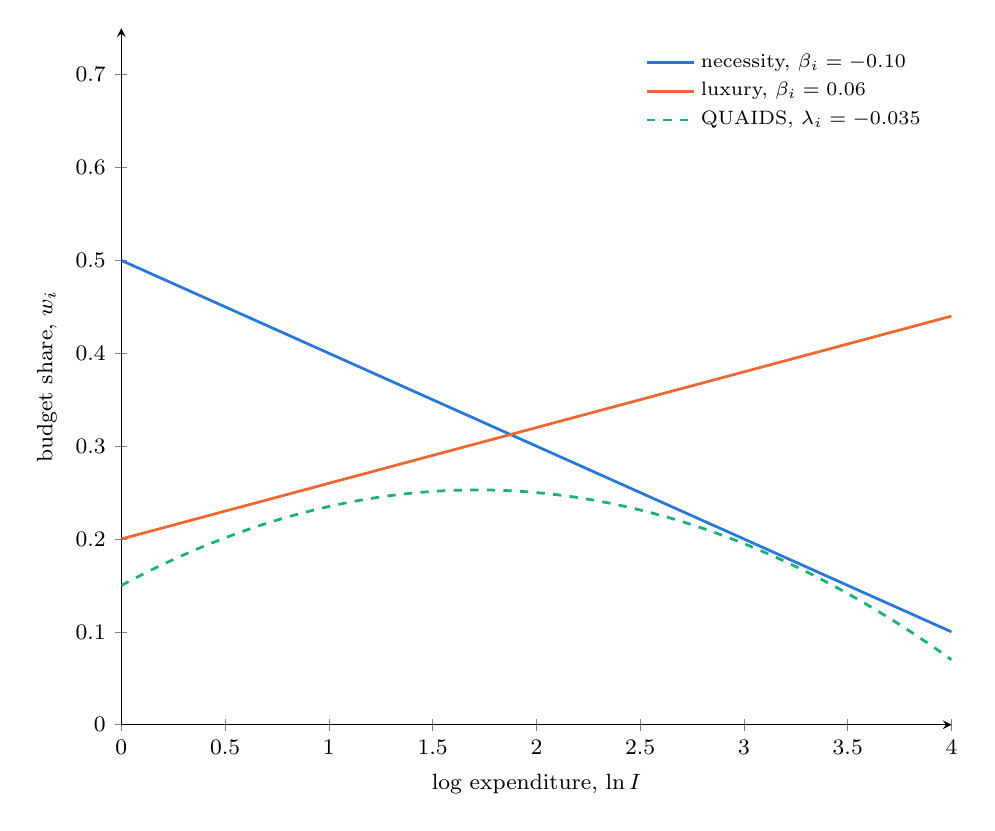
\begin{tikzpicture}
\begin{axis}[
  width=\linewidth, height=0.86\linewidth,
  axis lines=left, xmin=0, xmax=4, ymin=0, ymax=0.75,
  xlabel={log expenditure, $\ln I$}, ylabel={budget share, $w_i$},
  every axis plot/.append style={line width=1pt},
  legend style={font=\scriptsize, draw=none, fill=none, at={(0.98,0.98)}, anchor=north east},
  legend cell align=left,
  tick label style={font=\footnotesize}, label style={font=\footnotesize}]
\addplot[c05p1blue, domain=0:4, samples=2] {0.5 - 0.10*x};
\addlegendentry{necessity, $\beta_i = -0.10$}
\addplot[c05p1orange, domain=0:4, samples=2] {0.2 + 0.06*x};
\addlegendentry{luxury, $\beta_i = 0.06$}
\addplot[c05p1aqua, dashed, domain=0:4, samples=80] {0.15 + 0.12*x - 0.035*x^2};
\addlegendentry{QUAIDS, $\lambda_i = -0.035$}
\end{axis}
\end{tikzpicture}
\caption{Budget shares}\label{fig:05-engel-shares}
\end{subfigure}\hfill
\begin{subfigure}[t]{0.485\textwidth}
\centering
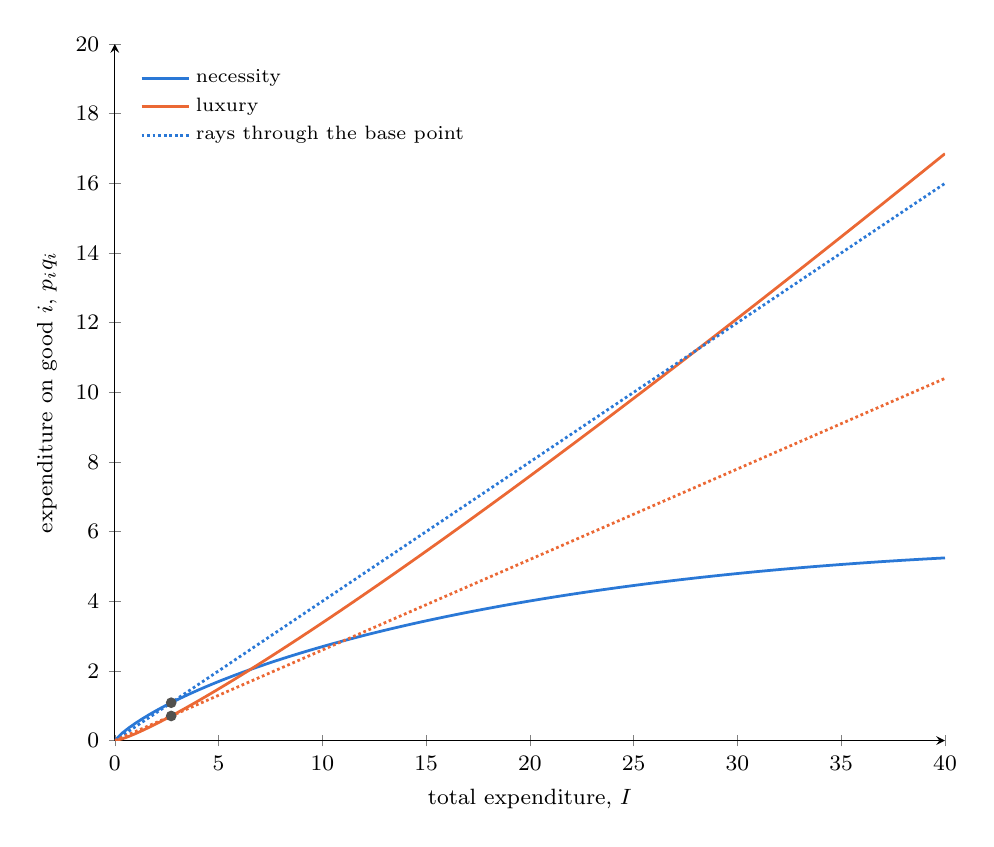
\begin{tikzpicture}
\begin{axis}[
  width=\linewidth, height=0.86\linewidth,
  axis lines=left, xmin=0, xmax=40, ymin=0, ymax=20,
  xlabel={total expenditure, $I$}, ylabel={expenditure on good $i$, $p_iq_i$},
  every axis plot/.append style={line width=1pt},
  legend style={font=\scriptsize, draw=none, fill=none, at={(0.02,0.98)}, anchor=north west},
  legend cell align=left,
  tick label style={font=\footnotesize}, label style={font=\footnotesize}]
\addplot[c05p1blue, domain=0.01:40, samples=120] {x*(0.5 - 0.10*ln(x))};
\addlegendentry{necessity}
\addplot[c05p1orange, domain=0.01:40, samples=120] {x*(0.2 + 0.06*ln(x))};
\addlegendentry{luxury}
\addplot[c05p1blue, densely dotted, domain=0:40, samples=2] {0.40*x};
\addlegendentry{rays through the base point}
\addplot[c05p1orange, densely dotted, domain=0:40, samples=2] {0.26*x};
\addplot[only marks, mark=*, mark size=1.4pt, c05p1gray] coordinates {(2.71828,1.08731) (2.71828,0.70675)};
\end{axis}
\end{tikzpicture}
\caption{Expenditure}\label{fig:05-engel-spending}
\end{subfigure}
\caption{Engel curves at unit prices. Panel (a) plots budget shares against $\ln I$ for good 1 of the running
example (a necessity, $w_1 = 0.5 - 0.10\ln I$), good 3 (a luxury, $w_3 = 0.2 + 0.06\ln I$), and an
illustrative QUAIDS good with $w = 0.15 + 0.12\ln I - 0.035(\ln I)^2$. The QUAIDS share rises until
$\ln I = \frac{0.12}{0.07} \approx 1.71$ and falls afterwards. Panel (b) plots the corresponding expenditures
$p_iq_i = w_iI$ for the two AIDS goods. The dotted rays are the homothetic Engel curves through the base point
$\ln I = 1$ (dots), where $w_1 = 0.40$ and $w_3 = 0.26$.}\label{fig:05-engel}
\end{figure}

\subsection{Why only almost ideal}\label{sec:05-aids-limits}

\citet[p.~312]{DeatonMuellbauer1980a} list six properties that together recommend the AIDS. It gives an
arbitrary first-order approximation to any demand system (\cref{prop:05-flexible}). It satisfies the axioms
of choice exactly, given the restrictions (\cref{prop:05-restrictions}). It aggregates over consumers without
invoking parallel linear Engel curves (\cref{sec:05-aggregation}). Its functional form is consistent with
household budget data (\cref{sec:05-engel}). It is simple to estimate and largely avoids nonlinear estimation
(\cref{sec:05-stone}). Finally, homogeneity and symmetry can be tested through linear restrictions on fixed
parameters (\cref{sec:05-testing}). The Rotterdam and translog models each possess some of these properties,
but neither possesses all of them at once. The authors themselves add that the system, particularly in its
simple static form, is not to be regarded as ``a fully satisfactory explanation of consumers' behavior''
\citep[p.~312]{DeatonMuellbauer1980a}.

The system falls short of the ideal in five ways.

\emph{Concavity is not guaranteed.} By \cref{prop:05-negativity}, negativity depends on the data point and
cannot be imposed by linear restrictions. Estimated systems often violate it at some observations. At unit
prices the running example is concave over the whole range of $\ln I$ in which all its shares lie in
$[0, 1]$, but this must be checked for every estimate.

\emph{Fitted shares can leave the unit interval.} Shares are linear in $\ln I$ and quadratic in $\ln p$, and
these variables are unbounded. For extreme prices or incomes the fitted shares become negative or exceed one, and the cost
function then ceases to be a valid expenditure function. In the running example at unit prices, the share of
good 1 is $0.5 - 0.10\ln I$, which turns negative above $\ln I = 5$. The share of good 3 turns negative below
$\ln I = -\frac{0.2}{0.06} \approx -3.33$. The appendix of \citet[p.~324]{DeatonMuellbauer1980a} derives the
corresponding restrictions on the admissible region of incomes and prices for the PIGLOG class.

\emph{There are many parameters.} The matrix $\Gamma$ has $J^2$ elements. Symmetry leaves
$\frac{J(J+1)}{2}$, and homogeneity removes $J$ more, leaving
\begin{equation}\label{eq:05-param-count}
\frac{J(J+1)}{2} - J = \frac{J(J-1)}{2}
\end{equation}
free price coefficients, about $\frac{1}{2}J^2$. Adding up then determines the last row of $\Gamma$ from the
others, and the $\alpha_i$ and $\beta_i$ add $2(J - 1)$ free parameters, plus $\alpha_0$. With $J = 8$
groups the count gives 28 free $\gamma_{ij}$ and 14 free $\alpha_i$ and $\beta_i$, the numbers that
\citet[p.~318]{DeatonMuellbauer1980a} report for their British application (\cref{sec:05-dm-application}).
With $J = 100$ products the count of $\gamma$'s is 4{,}950. \citet[p.~315]{DeatonMuellbauer1980a} suggest
setting individual $\gamma_{ij}$ to zero when theory or evidence supports it. The share of each good in such a
pair is then independent of the other's price at constant real expenditure. Setting every $\gamma_{ij}$
to zero is too strong. The resulting model, $w_i = \alpha_i + \beta_i\ln\frac{I}{\mathbf{P}}$, was tested and
rejected by \citet{Deaton1978}. The restrictions of \citet{ChaudhuriGoldbergJia2006} in \cref{sec:05-cgj}
follow the middle path.

\emph{Engel curves have rank two.} Shares are linear in $\ln I$, so a good cannot switch from luxury to
necessity as income grows. QUAIDS (\cref{prop:05-quaids}) relaxes this.

\emph{The choke price can be finite.} When the own share falls with $\ln p_i$, the demand for the good reaches
zero at a finite price. This is not automatic. With $\beta_i = 0$ it requires $\gamma_{ii} < 0$. The food
equation of \cref{tab:05-dm-table1} has $\gamma_{11} = 0.186$, and there the food share rises with the food
price. In the running example, holding the other prices at one and income at $\ln I = 1$,
the share of good 3 falls to zero at $p_3 \approx 4.10$. A finite virtual price lets the estimated own and
cross effects determine the value of a good, instead of the functional form alone (\cref{sec:05-three-systems}). It also means that
welfare calculations extrapolate the estimated demand curve well beyond the observed prices.
\Cref{sec:05-welfare-virtual} develops both sides of this feature.

Most of these limits are the price of a system that is linear enough to estimate and flexible enough to
test. The rest of the chapter shows how applied work lives with them: by aggregating goods into groups and
budgeting in stages, by instrumenting prices, and by checking curvature and extrapolation explicitly.

\section{Aggregation across consumers}\label{sec:05-aggregation}

The AIDS of \cref{sec:05-aids} describes the choices of a single consumer. Most data in industrial
organization are aggregates: the sales of a product in a city and a month, or national spending on a
group of goods in a year. This section asks when such aggregates behave as if one consumer had chosen
them. The answer decides two things. It decides whether the share equations of \eqref{eq:05-aids-share}
can be fitted to market data, and whether the welfare measures of \cref{sec:05-cv-ev}, computed from the
fitted system, describe anyone's welfare.

We index households by $h = 1, \dots, H$. Household $h$ has total expenditure $I_h$, demands $q_{ih}$
and budget shares $w_{ih} = \frac{p_i q_{ih}}{I_h}$. All households face the same price vector $p$.
Mean expenditure is $\bar I = \frac{1}{H}\sum_h I_h$. Hicksian demands keep the notation $h_i(p,u)$ of
\cref{sec:05-duality}, always written with their arguments, so they cannot be confused with the household
index.

\subsection{The aggregation problem}\label{sec:05-agg-problem}

Aggregate demand for good $i$ is the sum of household demands,
\begin{equation}\label{eq:05-agg-demand}
  Q_i(p, I_1, \dots, I_H) = \sum_{h=1}^{H} q_{ih}(p, I_h).
\end{equation}
In general it depends on the whole distribution of expenditure. To see why, transfer a small amount
$\dd t$ of expenditure from household $h'$ to household $h$, holding total expenditure fixed. Aggregate
demand changes by
\begin{equation*}
  \dd Q_i = \left(\frac{\partial q_{ih}}{\partial I_h} - \frac{\partial q_{ih'}}{\partial I_{h'}}\right)\dd t .
\end{equation*}
The change is zero only if the two households have the same marginal propensity to spend on good $i$
at their current budgets. Rich and poor households usually differ in this respect, so redistribution
moves market demand even when total spending does not change.

We want two things at once. Households should be allowed to differ in income and in demographics,
because they do. Yet we would like market data to look as if one consumer had generated them. A
\emph{representative consumer} is a fictional utility-maximizing consumer whose demand, evaluated at
current prices and at a scalar summary of the expenditure distribution, equals aggregate demand. We call
the representative consumer \emph{normative} when, in addition, its expenditure function measures the
welfare of the population, for example as the sum of household compensating variations. The positive
property licenses estimating a demand system on aggregate data. The normative property licenses welfare
analysis with the estimated system. The next subsections show how far each property can be pushed.

\subsection{The Gorman polar form and exact aggregation}\label{sec:05-gorman}

\begin{definition}[Gorman polar form]\label{def:05-gorman}
Households' preferences have the \emph{Gorman polar form} if their expenditure functions can be written
as
\begin{equation}\label{eq:05-gorman-form}
  e_h(p, u_h) = a_h(p) + b(p)\, u_h , \qquad h = 1, \dots, H.
\end{equation}
Here each $a_h(p)$ and the common function $b(p) > 0$ are homogeneous of degree one in $p$. On the
maintained domain of prices and utilities, each $e_h$ is increasing and concave in $p$. Preferences of
this form are called \emph{quasi-homothetic}.
\end{definition}

The function $a_h$ may differ across households, for example with family size or age. The function $b$
must be common. Under these conditions each $e_h$ is a valid expenditure function on the maintained
domain, and it is increasing in $u_h$ because $b > 0$. A convenient sufficient condition is that each
$a_h$ and $b$ is positive, increasing and concave, with $u_h \ge 0$. Then $e_h$ inherits monotonicity and
concavity in $p$ from $a_h$ and $b$. This subclass has $\frac{\partial \ln b}{\partial p_i} \ge 0$, which
by \eqref{eq:05-gorman-demand} below rules out inferior goods. The general form allows them on a local
domain. The name
reflects the relation to homotheticity. A homothetic expenditure function has the form $b(p)u$, so
budget shares do not depend on the budget. Adding the fixed cost $a_h(p)$ keeps Engel curves straight
but lets them miss the origin. The fixed cost is subsistence expenditure, the cost of living at $u_h = 0$
\citep[\S 5.4, pp.~142--144, and \S 6.1, eqs.~1.4--1.7, pp.~150--151]{DeatonMuellbauer1980b}.

\begin{proposition}[Exact aggregation, \citealp{Gorman1953,Gorman1961}]\label{prop:05-gorman}
Suppose every household has an interior optimum.
\begin{enumerate}[label=(\roman*)]
  \item If every household's expenditure function has the Gorman polar form \eqref{eq:05-gorman-form}
  with a common $b(p)$, aggregate demand depends on the distribution of expenditure only through
  $\sum_h I_h$. It is the demand of a representative consumer with expenditure function
  \begin{equation}\label{eq:05-gorman-rep}
    e(p, U) = \sum_{h=1}^{H} a_h(p) + b(p)\, U ,
  \end{equation}
  and the compensating variation of this consumer for any price change equals the sum of the
  households' compensating variations.
  \item Conversely, suppose aggregate demand depends only on $p$ and $\sum_h I_h$ for all distributions
  of expenditure in an open set. Then on that set household Engel curves are straight lines with slopes
  common to all households, and preferences have the Gorman polar form with a common $b(p)$. This $b$
  need not be increasing or concave.
\end{enumerate}
\end{proposition}

\begin{proof}
(i) Inverting $I_h = e_h(p, u_h)$ gives the indirect utility function
\begin{equation*}
  v_h(p, I_h) = \frac{I_h - a_h(p)}{b(p)} .
\end{equation*}
Roy's identity (\cref{prop:05-roy}) uses two partial derivatives:
\begin{align*}
  \frac{\partial v_h}{\partial I_h} &= \frac{1}{b(p)}, \\
  \frac{\partial v_h}{\partial p_i} &= -\frac{1}{b(p)}\frac{\partial a_h}{\partial p_i}
     - \frac{I_h - a_h(p)}{b(p)^2}\frac{\partial b}{\partial p_i} .
\end{align*}
Taking minus their ratio,
\begin{equation}\label{eq:05-gorman-demand}
  q_{ih}(p, I_h) = -\frac{\partial v_h}{\partial p_i}\left(\frac{\partial v_h}{\partial I_h}\right)^{-1}
  = \frac{\partial a_h}{\partial p_i} + \frac{\partial \ln b}{\partial p_i}\bigl(I_h - a_h(p)\bigr).
\end{equation}
The marginal propensity to spend, $\frac{\partial q_{ih}}{\partial I_h} = \frac{\partial \ln b}{\partial
p_i}$, depends on prices alone. It is the same for every household and at every budget. Summing
\eqref{eq:05-gorman-demand} over households gives
\begin{equation*}
  Q_i = \sum_h \frac{\partial a_h}{\partial p_i}
      + \frac{\partial \ln b}{\partial p_i}\Bigl(\sum_h I_h - \sum_h a_h(p)\Bigr),
\end{equation*}
which depends on budgets only through their sum.

Define $A(p) = \sum_h a_h(p)$ and $U = \sum_h u_h$. The function $e(p, U) = A(p) + b(p)U$ equals
$\sum_h e_h(p, u_h)$. It is therefore homogeneous of degree one, increasing and concave in $p$, and
increasing in $U$, so it is an expenditure function.
By Shephard's lemma (\cref{prop:05-shephard}) its Hicksian demand for good $i$ is $\frac{\partial
A}{\partial p_i} + \frac{\partial b}{\partial p_i}U$, the sum of the household Hicksian demands. Its
indirect utility at the total budget is $\frac{\sum_h I_h - A(p)}{b(p)} = \sum_h v_h(p, I_h)$, and Roy's
identity applied to it reproduces $Q_i$.

For a price change from $p^0$ to $p^1$, with initial utilities $u_h^0$, household $h$ has
\begin{equation*}
  CV_h = e_h(p^1, u_h^0) - e_h(p^0, u_h^0) = a_h(p^1) - a_h(p^0) + \bigl[b(p^1) - b(p^0)\bigr] u_h^0 .
\end{equation*}
Summing over households gives
\begin{equation*}
  \sum_h CV_h = A(p^1) - A(p^0) + \bigl[b(p^1) - b(p^0)\bigr] U^0 = e(p^1, U^0) - e(p^0, U^0),
\end{equation*}
the compensating variation of the representative consumer.

(ii) We sketch the argument. If $Q_i$ depends only on $\sum_h I_h$, every transfer between two
households leaves it unchanged. By the transfer argument of \cref{sec:05-agg-problem},
$\frac{\partial q_{ih}}{\partial I_h} = \frac{\partial q_{ih'}}{\partial I_{h'}}$ for every pair of
households and every pair of budgets in the open set. Fix the budget of $h'$ and vary that of $h$. The
derivative of $q_{ih}$ does not change, so it is a function $c_i(p)$ of prices alone, common to all
households. Integrating gives straight Engel curves $q_{ih} = d_{ih}(p) + c_i(p) I_h$. Recovering
preferences from these demands, with the symmetry and homogeneity restrictions of
\cref{prop:05-slutsky}, yields the Gorman polar form \citep{Gorman1961}.
\end{proof}

\begin{example}[The linear expenditure system]\label{ex:05-les}
The linear expenditure system of \citet{Stone1954} has expenditure function
\begin{equation*}
  e_h(p, u_h) = \sum_k p_k \underline{q}_{kh} + u_h \prod_k p_k^{m_k},
  \qquad m_k > 0, \quad \sum_k m_k = 1 ,
\end{equation*}
where $\underline{q}_{kh}$ is the subsistence quantity of good $k$ for household $h$. It has the Gorman
polar form with $a_h(p) = \sum_k p_k\underline{q}_{kh}$ and $b(p) = \prod_k p_k^{m_k}$. Since
$\frac{\partial \ln b}{\partial p_i} = \frac{m_i}{p_i}$, the demand function \eqref{eq:05-gorman-demand}
becomes
\begin{equation*}
  p_i q_{ih} = p_i \underline{q}_{ih} + m_i\Bigl(I_h - \sum_k p_k \underline{q}_{kh}\Bigr).
\end{equation*}
Each household first buys its subsistence bundle and then spends the fraction $m_i$ of its remaining
budget on good $i$. Households differ in subsistence quantities but share the marginal budget shares
$m_i$. Panel (a) of \cref{fig:05-gorman-piglog} draws two such Engel curves.
\end{example}

Exact aggregation comes at a price. Engel curves that are straight lines imply budget shares that
converge to constants as budgets grow and that leave the unit interval at low budgets. Household budget
surveys favor the Working-Leser form instead, in which budget shares are linear in the logarithm of the
budget (\cref{sec:05-engel}). Under that form the marginal propensity to spend changes with the budget,
as panel (b) of \cref{fig:05-gorman-piglog} shows, so a transfer between households moves aggregate
demand. We therefore want to relax linear Engel curves while keeping as much of the representative
consumer as possible.

Nonnegativity of demand breaks linear aggregation even when every household has quasi-homothetic
preferences \citep[\S 6.1, pp.~150--153]{DeatonMuellbauer1980b}. Fix prices and write a household's
Engel curve for one good as $q_h = d + cI_h$ with $c > 0$. If $d < 0$, the line implies negative demand
below the budget $I^* = -\frac{d}{c}$. Actual demand is zero there, so the true Engel curve is the
kinked line $q_h = \max\{0, c(I_h - I^*)\}$. A transfer from a household above the kink to one below it
lowers market demand, because the two have marginal propensities $c$ and $0$. Market demand then depends
on how many households sit below the kink. To see the shape, let budgets be uniform on $[\bar I -
\frac{r}{2}, \bar I + \frac{r}{2}]$, with $I^*$ inside this interval. Mean demand is
\begin{equation*}
  \bar q = \frac{1}{r}\int_{I^*}^{\bar I + \frac{r}{2}} c\,(I - I^*)\,\dd I
         = \frac{c}{2r}\Bigl(\bar I + \frac{r}{2} - I^*\Bigr)^2 ,
\end{equation*}
which is quadratic in mean expenditure. Its slope $\frac{c}{r}(\bar I + \frac{r}{2} - I^*)$ rises with
$\bar I$ as households cross the kink, and it reaches $c$ once all of them buy. This is the quadratic
case of \citet[Exercise~6.5]{DeatonMuellbauer1980b}, written in our notation.

The argument matters most for narrowly defined goods. Many consumers buy none of a particular brand, so
much of the market response to a higher budget comes from new buyers entering the market. Deaton and
Muellbauer call this the ``extensive'' margin, as opposed to the ``intensive'' margin of buyers who buy
more (p.~153). It would be a coincidence if the household Engel curves had just the offsetting
nonlinearity that made market demand linear. The discrete-choice models of \cref{ch:discrete,ch:logit}
put this extensive margin at the center, since each consumer there buys one product or none.

\begin{figure}[htbp]
\centering
\begin{subfigure}[t]{0.48\textwidth}
\centering
\begin{tikzpicture}
\begin{axis}[width=0.96\linewidth, height=0.84\linewidth,
  xmin=0, xmax=10.5, ymin=0, ymax=4.8,
  xlabel={total expenditure $I_h$}, ylabel={quantity of good 1, $q_{1h}$},
  xlabel style={font=\small}, ylabel style={font=\small}, tick label style={font=\scriptsize},
  axis lines=left, legend pos=north west, legend cell align=left,
  legend style={font=\scriptsize, draw=none, fill=none}]
  \addplot[thick, domain=1.5:10, samples=2] {0.55 + 0.3*x};
  \addplot[thick, dashed, domain=2.5:10, samples=2] {1.25 + 0.3*x};
  \addplot[only marks, mark=*, mark size=1.4pt, forget plot] coordinates {(1.5,1.0) (2.5,2.0)};
  \legend{household A, household B}
  \node[font=\scriptsize, align=left, anchor=north west] at (axis cs:3.6,1.3)
     {common slope $\frac{\partial q_{1h}}{\partial I_h} = \frac{m_1}{p_1}$};
\end{axis}
\end{tikzpicture}
\caption{Gorman polar form (linear expenditure system).}
\end{subfigure}\hfill
\begin{subfigure}[t]{0.48\textwidth}
\centering
\begin{tikzpicture}
\begin{axis}[width=0.96\linewidth, height=0.84\linewidth,
  xmin=0, xmax=8.5, ymin=0, ymax=2.8,
  xlabel={total expenditure $I_h$}, ylabel={quantity of good 1, $q_{1h}$},
  xlabel style={font=\small}, ylabel style={font=\small}, tick label style={font=\scriptsize},
  axis lines=left, legend pos=north west, legend cell align=left,
  legend style={font=\scriptsize, draw=none, fill=none}]
  \addplot[thick, domain=0.02:8, samples=120] {x*(0.5 - 0.10*ln(x))};
  \addplot[thin, dashed, domain=0:3.5, samples=2] {0.1 + 0.4*x};
  \addplot[thin, dashed, domain=1:8, samples=2, forget plot] {0.3 + 0.290139*x};
  \addplot[only marks, mark=*, mark size=1.4pt, forget plot] coordinates {(1,0.5) (3,1.170417)};
  \legend{AIDS Engel curve, tangents}
  \node[font=\scriptsize, anchor=north west] at (axis cs:1.05,0.45) {slope 0.40};
  \node[font=\scriptsize, anchor=north west] at (axis cs:3.05,1.12) {slope 0.29};
\end{axis}
\end{tikzpicture}
\caption{AIDS at unit prices (running example).}
\end{subfigure}
\caption{Engel curves under exact and almost exact aggregation. Panel (a): two households with the
linear expenditure system of \cref{ex:05-les}, $p = (1,1)$, $m_1 = 0.3$, subsistence quantities
$(\underline{q}_{1h}, \underline{q}_{2h}) = (1, 0.5)$ for household A (solid) and $(2, 0.5)$ for household
B (dashed). The lines start at the subsistence budgets (dots) and are parallel. Panel (b): the Engel curve
of good 1 in the running example of \cref{ex:05-running} at $p = (1,1,1)$, $q_1 = I(0.5 - 0.10\ln I)$. The
dashed tangents at the budgets $I = 1$ and $I = 3$ of the two households in \cref{ex:05-aggregation} have
slopes $0.4 - 0.10\ln I$, equal to 0.40 and 0.29. These are the households' marginal propensities to spend
on good 1. A transfer from the richer to the poorer household therefore raises aggregate demand for good
1. \Cref{fig:05-engel} draws the same curve together with a luxury.}
\label{fig:05-gorman-piglog}
\end{figure}

\subsection{Muellbauer's generalization: PIGL and PIGLOG}\label{sec:05-pigl}

\citet{Muellbauer1975,Muellbauer1976} weakens the requirement. The aggregate budget share of good $i$ is
aggregate spending on $i$ divided by aggregate spending. It equals the expenditure-weighted mean of
household shares:
\begin{equation}\label{eq:05-wbar}
  \bar w_i \equiv \frac{\sum_h p_i q_{ih}}{\sum_h I_h} = \sum_h \frac{I_h}{H\bar I}\, w_{ih}(p, I_h).
\end{equation}
Muellbauer's representative consumer exists if there is a scalar $I_0$, a function of prices and of the
distribution $(I_1, \dots, I_H)$, such that
\begin{equation}\label{eq:05-muellbauer}
  \bar w_i = w_i\bigl(p, I_0(p, I_1, \dots, I_H)\bigr) \quad \text{for every good } i.
\end{equation}
Here $w_i(p, \cdot)$ is the share function of a reference household
\citep[eq.~A1]{DeatonMuellbauer1980a}. We call $I_0$ the \emph{representative budget level}. The Gorman
case has $I_0 = \bar I$. Allowing $I_0$ to differ from the mean lets features of the distribution other
than its mean enter aggregate demand.

Muellbauer shows that \eqref{eq:05-muellbauer} holds if and only if household shares have the
\emph{generalized linear} form
\begin{equation}\label{eq:05-gl}
  w_{ih}(p, I_h) = v_h(p, I_h)\, A_i(p) + B_i(p) + \frac{C_{ih}(p)}{I_h},
\end{equation}
with $\sum_i A_i = \sum_i C_{ih} = \sum_h C_{ih} = 0$ and $\sum_i B_i = 1$
\citep[eq.~A2]{DeatonMuellbauer1980a}. The household-specific term $C_{ih}$ is an amount of spending, so it
enters the share divided by $I_h$. In the weighted mean \eqref{eq:05-wbar} it contributes $\frac{1}{H\bar
I}\sum_h C_{ih} = 0$.\footnote{\citet[eq.~A2]{DeatonMuellbauer1980a} print the term as $C_{ih}(p)$ with
$\sum_h C_{ih} = 0$. Read literally as a share term, it would leave $\sum_h \frac{I_h}{H\bar I}\,
C_{ih}$ in \eqref{eq:05-wbar}, which vanishes only if $\sum_h I_h C_{ih} = 0$. We write the term over
$I_h$, which is the reading under which it cancels.} We drop the household-specific terms $C_{ih}$ from
here on.

The preferences behind \eqref{eq:05-gl} have a simple structure \citep[\S 6.2, eqs.~2.3--2.6,
pp.~154--155]{DeatonMuellbauer1980b}. Household expenditure functions take the form $e_h(p, u_h) =
\theta_h[u_h, a(p), b(p)] + \phi_h(p)$. Here $a(p)$ and $b(p)$ are linearly homogeneous price indices
common to all households, and each $\theta_h$ is linearly homogeneous in $(a, b)$. The terms $\phi_h$ must
sum to zero over households, so the representative expenditure function is $e(p, u_0) = \theta[u_0,
a(p), b(p)]$. We can think of $a$ and $b$ as the prices of two intermediate goods. Shephard's lemma in
share form and the chain rule give
\begin{equation*}
  \bar w_i = \frac{\partial\ln\theta}{\partial\ln a}\,\frac{\partial\ln a}{\partial\ln p_i}
           + \frac{\partial\ln\theta}{\partial\ln b}\,\frac{\partial\ln b}{\partial\ln p_i} .
\end{equation*}
Euler's theorem for the degree-one function $\theta$ gives $\frac{\partial\ln\theta}{\partial\ln a} +
\frac{\partial\ln\theta}{\partial\ln b} = 1$. Writing $\varrho(I_0, p) = \frac{\partial\ln\theta}{\partial
\ln b}$ after substituting for $u_0$,
\begin{equation}\label{eq:05-gl-shares}
  \bar w_i = \bigl[1 - \varrho(I_0, p)\bigr]\frac{\partial\ln a}{\partial\ln p_i}
           + \varrho(I_0, p)\,\frac{\partial\ln b}{\partial\ln p_i} .
\end{equation}
Every aggregate share is a weighted average of the shares of the two indices, with one weight common to
all goods. Matching terms with \eqref{eq:05-gl} gives $B_i = \frac{\partial\ln a}{\partial\ln p_i}$, $A_i
= \frac{\partial\ln b}{\partial\ln p_i} - \frac{\partial\ln a}{\partial\ln p_i}$ and $v(p, I_0) =
\varrho(I_0, p)$. Hence
at constant prices each aggregate share is a linear function of every other share. With time-series data
in which relative prices barely move, this implication can be tested directly (p.~155).

The representative budget level is independent of prices if and only if
\begin{equation}\label{eq:05-pigl}
  v_h(p, I_h) = \frac{1 - \left(\frac{I_h}{\kappa_h}\right)^{-\psi}}{\psi}.
\end{equation}
Here $\psi$ is a constant and $\kappa_h > 0$ is a household-specific scale that does not depend on $I_h$
or $p$.\footnote{\citet[eq.~A3]{DeatonMuellbauer1980a} write the PIGL constant as $\alpha$. We use $\psi$
because $\alpha_i$ denotes the AIDS intercepts, and $\kappa_h$ for their $k_h$ because $k$ indexes goods.
The factor $\psi^{-1}$ appears in their typesetting as a superscript. We read it as a multiplicative
factor, which is the reading under which the limit $\psi \to 0$ gives their eq.~(A4).} Shares of this form
are called \emph{price-independent generalized linear} (PIGL). As $\psi \to 0$,
$\frac{1}{\psi}\bigl[1 - \exp\bigl(-\psi\ln\frac{I_h}{\kappa_h}\bigr)\bigr] \to \ln\frac{I_h}{\kappa_h}$, so
\begin{equation}\label{eq:05-piglog-v}
  v_h(p, I_h) = \ln \frac{I_h}{\kappa_h}.
\end{equation}
This limit is the \emph{price-independent generalized logarithmic} (PIGLOG) case.

\casehead{The representative budget level under PIGL}
With $C_{ih} = 0$, substituting \eqref{eq:05-gl} into \eqref{eq:05-wbar} gives
\begin{equation*}
  \bar w_i = A_i(p) \sum_h \frac{I_h}{H\bar I}\, v_h(p, I_h) + B_i(p).
\end{equation*}
A reference household with $\kappa = 1$ reproduces $\bar w_i$ if and only if $v(p, I_0) = \sum_h
\frac{I_h}{H\bar I} v_h(p, I_h)$. Under \eqref{eq:05-pigl} this condition reads
\begin{equation*}
  \frac{1 - I_0^{-\psi}}{\psi} = \sum_h \frac{I_h}{H\bar I}\,
  \frac{1 - \left(\frac{I_h}{\kappa_h}\right)^{-\psi}}{\psi} .
\end{equation*}
The weights $\frac{I_h}{H\bar I}$ sum to one, so the constant terms cancel and
\begin{equation}\label{eq:05-I0-pigl}
  I_0 = \left[\sum_h \frac{I_h}{H\bar I}\left(\frac{I_h}{\kappa_h}\right)^{-\psi}\right]^{-\frac{1}{\psi}} .
\end{equation}
The right-hand side involves budgets only, never prices. This is equation (A5) of
\citet{DeatonMuellbauer1980a}.\footnote{The version printed in their appendix omits the weight $I_h$
inside the sum. With the weight, $I_0$ equals the common budget when all budgets are equal and
$\kappa_h = 1$, as it must. Their book prints the formula with the weight. For $\kappa_h = 1$ it reads
$I_0 = \bigl[\frac{\sum_h I_h^{1-\psi}}{\sum_h I_h}\bigr]^{-\frac{1}{\psi}}$ \citep[\S 6.2, eq.~2.13,
p.~156]{DeatonMuellbauer1980b}, which is \eqref{eq:05-I0-pigl}.} Letting $\psi \to 0$ and expanding
$(\frac{I_h}{\kappa_h})^{-\psi} \approx 1 - \psi\ln\frac{I_h}{\kappa_h}$ gives the PIGLOG representative
budget,
\begin{equation}\label{eq:05-I0-piglog}
  \ln I_0 = \sum_h \frac{I_h}{H\bar I}\ln\frac{I_h}{\kappa_h}.
\end{equation}

The curvature parameter $\psi$ fixes how the distribution of budgets enters $I_0$. Take $\kappa_h = 1$.
Then \eqref{eq:05-I0-pigl} says that $I_0$ is a power mean of order $-\psi$ of the budgets, with
expenditure weights $\frac{I_h}{H\bar I}$. Power means rise with their order, so $I_0$ falls as $\psi$
rises. At $\psi = 1$, the case of linear Engel curves, the weighted mean of order $-1$ is
\begin{equation*}
  I_0 = \Bigl[\sum_h \frac{I_h}{H\bar I}\cdot\frac{1}{I_h}\Bigr]^{-1} = \Bigl[\frac{H}{H\bar I}\Bigr]^{-1}
      = \bar I ,
\end{equation*}
as in the Gorman case. Hence, when budgets are unequal, $I_0 > \bar I$ exactly when $\psi < 1$, the
empirically relevant case. Two
values of $\psi$ give closed forms \citep[\S 6.2, eqs.~2.14--2.15, p.~157]{DeatonMuellbauer1980b}. At
$\psi = -1$ the shares \eqref{eq:05-pigl-shares} are linear in the budget, so spending on each good is
quadratic in it. Then
\begin{equation*}
  I_0 = \frac{\sum_h I_h^2}{\sum_h I_h} = \frac{H(\sigma^2 + \bar I^2)}{H\bar I}
      = \bar I\Bigl(1 + \frac{\sigma^2}{\bar I^2}\Bigr),
\end{equation*}
where $\sigma^2 = \frac{1}{H}\sum_h (I_h - \bar I)^2$ is the variance of budgets. The representative budget
exceeds the mean by a factor of one plus the squared coefficient of variation. In the PIGLOG limit,
\cref{sec:05-almost-exact} shows that $\frac{I_0}{\bar I} = \frac{H}{Z}$, where $\ln Z$ is Theil's entropy
measure.
Deaton and Muellbauer's book writes this ratio as $\kappa_0 = \frac{I_0}{\bar I}$. It is the inverse of the
index $\kappa = \frac{Z}{H}$ of their article and of \cref{prop:05-almost-exact}.

\casehead{Cost functions and budget shares}
If household behavior comes from preferences, the PIGL cost function takes the form
\begin{equation}\label{eq:05-pigl-cost}
  \left[\frac{e(p, u_h)}{\kappa_h}\right]^{\psi} = (1 - u_h)\, a(p)^{\psi} + u_h\, b(p)^{\psi},
\end{equation}
and as $\psi \to 0$ it becomes the PIGLOG form
\begin{equation}\label{eq:05-piglog-cost}
  \ln\frac{e(p, u_h)}{\kappa_h} = (1 - u_h) \ln a(p) + u_h \ln b(p)
\end{equation}
\citep[eqs.~A6--A7]{DeatonMuellbauer1980a}. Here $a(p)$ and $b(p)$ are linearly homogeneous and concave,
and $0 \le u_h \le 1$ except as discussed below. With $\kappa_h = 1$, \eqref{eq:05-piglog-cost} is the
PIGLOG family of \cref{sec:05-piglog}.

The budget shares follow from Shephard's lemma in share form, $w_i = \frac{\partial \ln e}{\partial \ln
p_i}$. Take $\kappa_h = 1$, drop the household subscript, and write $a_i = \frac{\partial \ln a}{\partial
\ln p_i}$ and $b_i = \frac{\partial \ln b}{\partial \ln p_i}$. Differentiating \eqref{eq:05-pigl-cost}
with respect to $\ln p_i$, and using $\frac{\partial e^{\psi}}{\partial \ln p_i} = \psi e^{\psi}
\frac{\partial \ln e}{\partial \ln p_i}$, gives
\begin{equation*}
  \psi e^{\psi}\frac{\partial \ln e}{\partial \ln p_i} = (1 - u)\,\psi a^{\psi} a_i + u\, \psi b^{\psi} b_i .
\end{equation*}
At the optimum $e = I$. Dividing by $\psi I^{\psi}$,
\begin{equation}\label{eq:05-pigl-shares}
  w_i = (1 - u)\left(\frac{a}{I}\right)^{\psi} a_i + u\left(\frac{b}{I}\right)^{\psi} b_i,
  \qquad u = \frac{I^{\psi} - a^{\psi}}{b^{\psi} - a^{\psi}} .
\end{equation}
In the PIGLOG limit,
\begin{equation}\label{eq:05-piglog-shares}
  w_i = (1 - u)\, a_i + u\, b_i, \qquad u = \frac{\ln I - \ln a}{\ln b - \ln a}
\end{equation}
\citep[eqs.~A8--A10]{DeatonMuellbauer1980a}.

These equations have a transparent reading. By \eqref{eq:05-pigl-cost}, $(1-u)a^{\psi} + ub^{\psi} =
I^{\psi}$, so the weights $(1-u)(\frac{a}{I})^{\psi}$ and $u(\frac{b}{I})^{\psi}$ sum to one. Budget
shares are weighted averages of $a_i$ and $b_i$. As utility rises from $0$ to $1$, cost rises from $a(p)$
to $b(p)$ whenever $b > a$, whatever the sign of $\psi$, and the shares move from $a_i$ to $b_i$.
\citet{DeatonMuellbauer1980a} call $a(p)$ ``poverty'' expenditure, with spending pattern $a_i$, and $b(p)$
``affluence'' expenditure, with pattern $b_i$. A good is a luxury if and only if $b_i > a_i$, because its
share then rises with $u$. Inferior goods are not excluded.

For the AIDS, \eqref{eq:05-aids-cost} gives $\ln a(p) = \ln\mathbf{P}(p)$ and $\ln b(p) = \ln a(p) +
\beta_0\prod_k p_k^{\beta_k}$. Because $\frac{\partial}{\partial \ln p_i}\prod_k p_k^{\beta_k} = \beta_i
\prod_k p_k^{\beta_k}$,
\begin{equation*}
  b_i - a_i = \beta_i\, \beta_0 \prod_k p_k^{\beta_k}.
\end{equation*}
With $\beta_0 > 0$, good $i$ is a luxury exactly when $\beta_i > 0$, as found in \cref{sec:05-aids}.

\casehead{Where the demands are valid}
Shares must lie in $[0, 1]$. Under PIGLOG each $w_i$ is linear in $u$, so the admissible values of $u$
form an interval. Because $a(p)$ and $b(p)$ are increasing and linearly homogeneous, $a_i \ge 0$, $b_i
\ge 0$ and $\sum_i a_i = \sum_i b_i = 1$. Hence $a_i, b_i \in [0,1]$, and every $u \in [0,1]$ is
admissible. Above $u = 1$, the share of a luxury reaches one at $u = \frac{1 - a_i}{b_i - a_i}$, and the
share of a necessity reaches zero at $u = \frac{a_i}{a_i - b_i}$. The upper end of the admissible
interval is the smallest of these values. Below $u = 0$ the same reasoning, with the roles of zero and
one exchanged, gives the lower end. \citet[p.~324]{DeatonMuellbauer1980a} state the corresponding limits
for the PIGL case.

In the running example at unit prices, $\ln a = \alpha_0 = 0$ and $\ln b - \ln a = \beta_0 = 1$, so $u =
\ln I$. The share vectors are $a = \alpha = (0.5, 0.3, 0.2)$ and $b = \alpha + \beta = (0.40, 0.34, 0.26)$.
The necessity, good 1, has its share reach zero at $u = \frac{0.5}{0.1} = 5$. Goods 2 and 3 reach a share
of one only at $u = 17.5$ and $u = 13.3$. Below zero, the share of good 3 reaches zero first, at $u =
-\frac{0.2}{0.06} = -3.33$. The demands are therefore valid for $\ln I \in [-3.33, 5]$, the range reported
for the running example in \cref{sec:05-aids-limits}.

\casehead{Concavity}
A sufficient condition for the PIGLOG cost function to be concave in $p$ is that $a$ and $b$ be concave
and $0 \le u \le 1$. To see this, write \eqref{eq:05-piglog-cost} as $e = a(p)^{1-u}\, b(p)^{u}$. The
weighted geometric mean $g(x, y) = x^{1-u}y^{u}$ is concave and nondecreasing on the positive orthant for
$u \in [0, 1]$. A concave nondecreasing function of concave functions is concave. The condition is not
necessary. \citet[p.~324]{DeatonMuellbauer1980a} show that the PIGL cost function is concave for
\emph{all} $I > 0$ and $p > 0$ only if $a_i = b_i$ for every $i$, in which case preferences are
homothetic. Any nonhomothetic PIGLOG system, the AIDS included, must therefore have its concavity checked
where it is used, as in \cref{prop:05-negativity}.

\casehead{Two special cases}
With $\psi = 1$, \eqref{eq:05-pigl-cost} reads $e_h = \kappa_h a(p) + \kappa_h u_h[b(p) - a(p)]$. Defining
$\tilde u_h = \kappa_h u_h$ gives $e_h = \kappa_h a(p) + [b(p) - a(p)]\tilde u_h$, a Gorman polar form with
$a_h = \kappa_h a$ and common slope function $b - a$. So the PIGL family contains every model with linear
Engel curves, such as the linear expenditure system \citep[p.~324]{DeatonMuellbauer1980a}. The second
case is less obvious.

\begin{remark}[When the indirect translog is PIGLOG]\label{rem:05-translog-piglog}
The indirect translog of \citet{ChristensenJorgensonLau1975} specifies indirect utility as
\begin{equation*}
  v = \tau_0 + \sum_i \tau_i \ln\frac{p_i}{I}
      + \frac{1}{2}\sum_i\sum_j \tau_{ij}\ln\frac{p_i}{I}\ln\frac{p_j}{I},
\end{equation*}
with the normalizations $\sum_i \tau_i = -1$ and $\tau_{ij} = \tau_{ji}$. Let $\tau_{Mi} = \sum_k
\tau_{ki}$ and $L = \ln I$. Expanding the products and collecting powers of $L$,
\begin{equation*}
  v = \tau_0 + \sum_i \tau_i \ln p_i + \frac{1}{2}\sum_i\sum_j \tau_{ij}\ln p_i \ln p_j
      + L\Bigl(1 - \sum_i \tau_{Mi}\ln p_i\Bigr) + \frac{1}{2}L^2 \sum_i \tau_{Mi} .
\end{equation*}
If $\sum_i \tau_{Mi} = 0$, utility is linear in $L$ and can be solved for the log cost function:
\begin{equation*}
  \ln e(p, v) = \frac{v - \tau_0 - \sum_i \tau_i \ln p_i - \frac{1}{2}\sum_i\sum_j\tau_{ij}\ln p_i\ln p_j}
                     {1 - \sum_i \tau_{Mi}\ln p_i} .
\end{equation*}
This is linear in $v$, with an intercept and a slope that depend on prices, which is the PIGLOG form
\eqref{eq:05-piglog-cost}. If $\sum_i\tau_{Mi} \neq 0$, utility is quadratic in $L$ and $\ln e$ is not
linear in $v$. Utility is ordinal, so this alone does not exclude a PIGLOG form for some increasing
transformation of $v$. Budget shares do not depend on how utility is normalized, and they settle the
question. Write $\tau_{MM} = \sum_i\tau_{Mi}$, $N_i(p) = \tau_i + \sum_j\tau_{ij}\ln p_j$ and $D(p) =
\sum_j\tau_{Mj}\ln p_j - 1$. Roy's identity and the symmetry of $\tau_{ij}$ give
\begin{equation*}
  w_i = \frac{N_i(p) - \tau_{Mi}L}{D(p) - \tau_{MM}L}
      = \frac{\tau_{Mi}}{\tau_{MM}} + \frac{c_i(p)}{D(p) - \tau_{MM}L},
  \qquad c_i(p) = N_i(p) - \frac{\tau_{Mi}}{\tau_{MM}}D(p),
\end{equation*}
where the second form requires $\tau_{MM} \neq 0$. By \eqref{eq:05-pigl-shares}, PIGL shares are affine
in $I^{-\psi}$, and PIGLOG shares are affine in $L$. The last term has neither form on an interval of
budgets unless $c_i(p) = 0$. Matching the constant and the coefficients of $\ln p_j$ in $c_i(p) = 0$ gives
$\tau_{Mi} = -\tau_i\tau_{MM}$ and $\tau_{ij} = \tau_i\tau_j\tau_{MM}$, so that $w_i = -\tau_i$ at all
prices and budgets. These are Cobb-Douglas preferences. With $t = L + \sum_i\tau_i\ln p_i$, utility is
$v = \tau_0 + t + \frac{1}{2}\tau_{MM}t^2$, which represents them only where $1 + \tau_{MM}t > 0$.
Apart from this homothetic case, the indirect translog is PIGLOG exactly when $\tau_{MM} = 0$. For
$\tau_{MM} \neq 0$ the display still has the generalized linear form \eqref{eq:05-gl}, with
$v_h(p, I_h) = \frac{1}{D(p) - \tau_{MM}\ln I_h}$, $A_i = c_i(p)$ and $B_i = \frac{\tau_{Mi}}{\tau_{MM}}$.
Because $\sum_i N_i(p) = D(p)$, these satisfy $\sum_i c_i(p) = 0$ and $\sum_i B_i = 1$. A
representative budget level in the sense of \eqref{eq:05-muellbauer} then exists. The shares are
neither PIGL nor PIGLOG, so by \eqref{eq:05-pigl} that level depends on prices.
\citet[p.~325, eqs.~A11--A12]{DeatonMuellbauer1980a} call $\tau_{MM} = 0$ the only case in which the
indirect translog allows consistent aggregation. Their claim is right for a representative budget level
that does not depend on prices, apart from the homothetic exception, which they do not note. They add
that no such result holds for any interesting special case of the direct translog.
\end{remark}

\casehead{Evidence on the curvature parameter}
\citet[\S 6.2, p.~158]{DeatonMuellbauer1980b} fit the PIGL demand functions to postwar British data for
1954--1974 with eight groups of goods, the same period and number of groups as in
\cref{sec:05-dm-application}. They take $a(p) = \sum_k
a_kp_k$, the cost of a fixed subsistence bundle, and $b(p) = \beta_0\prod_k p_k^{\beta_k}$. The estimate of
$\psi$ is very close to $-1$, which implies nearly quadratic Engel curves over time. The hypothesis $\psi =
1$, which gives linear Engel curves, is decisively rejected. The book states these results in words and
reports no numerical estimate. A full use of the PIGL class would also measure $I_0$ from the
distribution of budgets. Few countries have data on the distribution of total expenditure of sufficient
quality for this, and the authors' own indirect attempts had no notable success. Applied work therefore
replaces $I_0$ by $\bar I$. The error is small if the distribution is stable, so that $\frac{I_0}{\bar I}$
is roughly constant, which they judge possible for postwar Britain (p.~158).
\Cref{sec:05-almost-exact} shows what the approximation costs when the distribution moves.

\subsection{Almost exact aggregation of the AIDS}\label{sec:05-almost-exact}

The AIDS is a PIGLOG system, so it aggregates through a single representative budget.
\citet[Section~I.A]{DeatonMuellbauer1980a} allow households to differ through a scale $\kappa_h$. They
interpret it as ``a sophisticated measure of household size'' that could reflect age composition, other
characteristics and economies of household size. Household $h$ deflates its budget by $\kappa_h$ to a
``needs corrected'' per capita level.

\begin{proposition}[Almost exact aggregation]\label{prop:05-almost-exact}
Suppose every household has the AIDS preferences of \eqref{eq:05-aids-cost} with common parameters, except
for a scale $\kappa_h > 0$ that deflates its budget, so that
\begin{equation}\label{eq:05-aids-household}
  w_{ih} = \alpha_i + \sum_j \gamma_{ij}\ln p_j + \beta_i \ln\frac{I_h}{\kappa_h \mathbf{P}(p)} .
\end{equation}
Define the aggregate index $\kappa$ by
\begin{equation}\label{eq:05-kappa}
  \ln\frac{\bar I}{\kappa} = \sum_h \frac{I_h}{H\bar I}\ln\frac{I_h}{\kappa_h}.
\end{equation}
Then the aggregate budget shares are
\begin{equation}\label{eq:05-aids-aggregate}
  \bar w_i = \alpha_i + \sum_j \gamma_{ij}\ln p_j + \beta_i \ln\frac{\bar I}{\kappa\, \mathbf{P}(p)} ,
\end{equation}
the shares of a single AIDS household with budget $\frac{\bar I}{\kappa}$. When $\kappa_h = 1$ for all
households, $\frac{\bar I}{\kappa} = I_0$ with
\begin{equation}\label{eq:05-I0}
  \ln I_0 = \frac{\sum_h I_h \ln I_h}{\sum_h I_h} .
\end{equation}
\end{proposition}

\begin{proof}
Let $A_i(p) = \alpha_i + \sum_j\gamma_{ij}\ln p_j - \beta_i\ln\mathbf{P}(p)$, so that $w_{ih} = A_i(p) +
\beta_i\ln\frac{I_h}{\kappa_h}$. Substitute into \eqref{eq:05-wbar}:
\begin{align*}
  \bar w_i &= \sum_h \frac{I_h}{H\bar I}\Bigl[A_i(p) + \beta_i\ln\frac{I_h}{\kappa_h}\Bigr] \\
           &= A_i(p)\sum_h \frac{I_h}{H\bar I} + \beta_i \sum_h \frac{I_h}{H\bar I}\ln\frac{I_h}{\kappa_h} \\
           &= A_i(p) + \beta_i\ln\frac{\bar I}{\kappa} .
\end{align*}
The last line uses the fact that the weights sum to one and the definition \eqref{eq:05-kappa}.
Substituting $A_i(p)$ back gives \eqref{eq:05-aids-aggregate}. With $\kappa_h = 1$, \eqref{eq:05-kappa}
reads $\ln\frac{\bar I}{\kappa} = \sum_h \frac{I_h}{H\bar I}\ln I_h$, which is \eqref{eq:05-I0}.
\end{proof}

The same argument works for any PIGLOG system. From \eqref{eq:05-piglog-shares}, $u_h = \frac{\ln I_h -
\ln a}{\ln b - \ln a}$, so
\begin{equation*}
  w_{ih} = a_i + (b_i - a_i)u_h
  = \Bigl[a_i - \frac{b_i - a_i}{\ln b - \ln a}\ln a\Bigr] + \frac{b_i - a_i}{\ln b - \ln a}\ln I_h .
\end{equation*}
Household shares are linear in $\ln I_h$ with price-dependent coefficients $A_i(p)$ and $B_i(p)$. For the
AIDS, $b_i - a_i = \beta_i(\ln b - \ln a)$, so $B_i = \beta_i$ and $A_i = a_i - \beta_i\ln a = \alpha_i +
\sum_j\gamma_{ij}\ln p_j - \beta_i\ln\mathbf{P}$, as in the proof. Aggregation is ``almost'' exact
because aggregate demand depends on the distribution of budgets, but only through one scalar index.

\casehead{What $I_0$ measures}
Write each budget as $I_h = \bar I\cdot\frac{I_h}{\bar I}$. Then
\begin{align}
  \ln I_0 &= \sum_h \frac{I_h}{H\bar I}\Bigl[\ln\bar I + \ln\frac{I_h}{\bar I}\Bigr]
           = \ln\bar I + \mathcal{T}, \notag\\
  \mathcal{T} &= \frac{1}{H}\sum_h \frac{I_h}{\bar I}\ln\frac{I_h}{\bar I}. \label{eq:05-theil}
\end{align}
The quantity $\mathcal{T}$ is the \emph{Theil index} of inequality. The function $f(r) = r\ln r$ is
convex and the ratios $r_h = \frac{I_h}{\bar I}$ average one. Jensen's inequality therefore gives
$\mathcal{T} = \frac{1}{H}\sum_h f(r_h) \ge f(1) = 0$, with equality only when all budgets are equal. The
maximum, $\ln H$, is reached when one household does all the spending. Hence
\begin{equation*}
  I_0 = \bar I\, e^{\mathcal{T}} \ge \bar I .
\end{equation*}
The representative household is richer than the average household, because expenditure weighting gives
rich households more weight.

Deaton and Muellbauer express the same object through an entropy measure. With $\kappa_h = 1$ they write
$\kappa = \frac{Z}{H}$, where $\ln Z = -\sum_h \frac{I_h}{H\bar I}\ln\frac{I_h}{H\bar I}$ is Theil's
entropy measure of equality. Since $\ln\frac{I_h}{H\bar I} = \ln\frac{I_h}{\bar I} - \ln H$,
\begin{equation*}
  \ln Z = \ln H - \mathcal{T}, \qquad \ln\kappa = \ln Z - \ln H = -\mathcal{T}, \qquad
  \frac{\bar I}{\kappa} = \bar I e^{\mathcal{T}} = I_0 .
\end{equation*}
Hence $\frac{I_0}{\bar I} = \frac{H}{Z}$, which is the ratio $\kappa_0$ of \citet[\S 6.2, eq.~2.15,
p.~157]{DeatonMuellbauer1980b}. The entropy $Z$ reaches its maximum $H$ under perfect equality. In their words, ``as inequality
increases, $k = \frac{Z}{H}$ decreases and the representative budget level increases''
\citep[p.~315]{DeatonMuellbauer1980a}. When the scales $\kappa_h$ differ across households, $\kappa$
reflects the demographic structure as well as the distribution of budgets.

\casehead{Consequences for estimation}
In a time series of aggregate shares, \eqref{eq:05-aids-aggregate} reads
\begin{equation}\label{eq:05-aids-agg-ts}
  \bar w_{it} = \alpha_i + \sum_j\gamma_{ij}\ln p_{jt} + \beta_i\ln\frac{\bar I_t}{\mathbf{P}_t}
                - \beta_i\ln\kappa_t .
\end{equation}
Researchers usually observe mean expenditure $\bar I_t$ but not $\kappa_t$, which requires the joint
distribution of budgets and household characteristics. If $\kappa_t$ is constant, or varies independently
of $\bar I_t$ and $p_t$, we can replace $\ln\kappa_t$ by a constant $\ln\kappa^*$, its value or sample
mean. The intercepts then become $\alpha_i^* = \alpha_i - \beta_i\ln\kappa^*$
\citep[p.~315]{DeatonMuellbauer1980a}. The deviation $-\beta_i(\ln\kappa_t - \ln\kappa^*)$ joins the
error term and is uncorrelated with the regressors.

If $\kappa_t$ moves with the regressors, omitting it biases the estimates. Take the case $\kappa_h = 1$,
so that $-\ln\kappa_t = \mathcal{T}_t$, and hold prices fixed for simplicity. Let the linear projection of
inequality on log mean expenditure be $\mathcal{T}_t = c + \delta_{\mathcal{T}}\ln\bar I_t + r_t$, with
$r_t$ uncorrelated with $\ln\bar I_t$. Substituting into \eqref{eq:05-aids-agg-ts} and adding an error
term $\xi_{it}$,
\begin{equation*}
  \bar w_{it} = \bigl(\alpha_i - \beta_i\ln\mathbf{P} + \beta_i c\bigr)
               + \beta_i(1 + \delta_{\mathcal{T}})\ln\bar I_t + \beta_i r_t + \xi_{it}.
\end{equation*}
A regression of $\bar w_{it}$ on $\ln\bar I_t$ estimates $\beta_i(1 + \delta_{\mathcal{T}})$. If
inequality rises with mean expenditure ($\delta_{\mathcal{T}} > 0$), luxuries look more luxurious and
necessities more necessary than they are. With several regressors the same logic applies to the partial
correlation of $\mathcal{T}_t$ with each of them. Deaton and Muellbauer list a non-constant $\kappa$
correlated with $\bar I$ and $p$ as one possible reason for the rejection of homogeneity in their data
(\cref{sec:05-dm-application}).

The index $\kappa$ is constant when the distribution of budgets and household characteristics changes
only through equiproportional changes in all budgets. Deaton and Muellbauer point out that in this case
even $\alpha_{ih}$ and $\gamma_{ijh}$ may differ across households. The reason is that the weights
$\frac{I_h}{H\bar I}$ are then constant over time, and each household's $\ln\mathbf{P}_h$ is linear in its
own parameters. With a common $\beta_i$, the weighted sum of the household equations is an AIDS whose
$\alpha_i$ and $\gamma_{ij}$ are expenditure-weighted averages of the household parameters.

\begin{example}[Two households]\label{ex:05-aggregation}
Take the running example of \cref{ex:05-running} at $p = (1,1,1)$, where $\ln\mathbf{P} = 0$ and $w_{ih} =
\alpha_i + \beta_i\ln I_h$. Two households have budgets $I_1 = 1$ and $I_2 = 3$, so $\bar I = 2$. The
expenditure weights are $\frac{1}{4}$ and $\frac{3}{4}$, and
\begin{equation*}
  \ln I_0 = \frac{1}{4}\ln 1 + \frac{3}{4}\ln 3 = 0.8240, \qquad I_0 = 2.280 .
\end{equation*}
The Theil index is $\mathcal{T} = \ln I_0 - \ln\bar I = 0.8240 - 0.6931 = 0.1308$. Equivalently,
$\kappa = e^{-\mathcal{T}} = 0.877$ and $Z = H\kappa = 1.755$. \Cref{tab:05-agg-example} reports the
household shares, the aggregate shares computed from \eqref{eq:05-wbar}, and the shares of a single
consumer at $I_0$ and at $\bar I$. The consumer with budget $I_0$ reproduces the aggregate shares
exactly. The consumer with the mean budget overstates the share of the necessity, good 1, by 1.3
percentage points and understates the share of the luxury, good 3, by 0.8 points.
\end{example}

\begin{table}[htbp]
\centering
\caption{Aggregation in the running example at unit prices}
\label{tab:05-agg-example}
\begin{tabular}{lccccc}
\toprule
 & Budget & $\ln$ budget & $w_1$ & $w_2$ & $w_3$ \\
\midrule
Household 1 & 1.000 & 0.0000 & 0.5000 & 0.3000 & 0.2000 \\
Household 2 & 3.000 & 1.0986 & 0.3901 & 0.3439 & 0.2659 \\
Aggregate, \eqref{eq:05-wbar} & 4.000 & & 0.4176 & 0.3330 & 0.2494 \\
Consumer at $I_0$ & 2.280 & 0.8240 & 0.4176 & 0.3330 & 0.2494 \\
Consumer at $\bar I$ & 2.000 & 0.6931 & 0.4307 & 0.3277 & 0.2416 \\
\bottomrule
\end{tabular}

\smallskip
\begin{minipage}{0.82\textwidth}
\footnotesize Notes: parameters of \cref{ex:05-running}, $w_{ih} = \alpha_i + \beta_i\ln I_h$ at $p =
(1,1,1)$. The aggregate row gives total expenditure and expenditure-weighted shares. Computed by
\texttt{figures/ch05/src/aggregation\_example.py}.
\end{minipage}
\end{table}

\begin{remark}[Welfare with a representative household]\label{rem:05-agg-welfare}
Under the Gorman polar form the representative consumer is normative: its compensating variation is the
sum of household compensating variations (\cref{prop:05-gorman}). Under PIGLOG the household with budget
$I_0$ is a positive construct, and its expenditure function does not aggregate the household expenditure
functions. How large is the error if we use it anyway? For the AIDS, the initial utility of household $h$
is $u_h^0 = \frac{\ln I_h - \ln\mathbf{P}(p^0)}{B(p^0)}$ by \eqref{eq:05-aids-v}, with $B(p) =
\beta_0\prod_k p_k^{\beta_k}$ as in \eqref{eq:05-aids-B}. Its cost of reaching $u_h^0$ at new prices $p^1$
satisfies
\begin{equation*}
  \ln e(p^1, u_h^0) = \ln\mathbf{P}(p^1) + g\bigl[\ln I_h - \ln\mathbf{P}(p^0)\bigr],
  \qquad g = \frac{B(p^1)}{B(p^0)} ,
\end{equation*}
so $e(p^1, u_h^0) = \mathbf{P}(p^1)\mathbf{P}(p^0)^{-g} I_h^{g}$. Summing over households gives
$\mathbf{P}(p^1)\mathbf{P}(p^0)^{-g}\sum_h I_h^g$. A natural representative calculation computes the
compensating variation of the household with budget $I_0$ as a fraction of its budget and applies that
fraction to aggregate expenditure $H\bar I$. This gives $\mathbf{P}(p^1)\mathbf{P}(p^0)^{-g} H\bar I\,
I_0^{g-1}$ for the aggregate cost at new prices. Since the exponential function is convex, Jensen's
inequality gives
\begin{equation*}
  \sum_h I_h^{g} = H\bar I\sum_h \frac{I_h}{H\bar I}\, e^{(g-1)\ln I_h}
  \ge H\bar I\, e^{(g-1)\sum_h \frac{I_h}{H\bar I}\ln I_h} = H\bar I\, I_0^{g-1}.
\end{equation*}
The representative calculation therefore understates the sum of household compensating variations. The
two coincide when $g = 1$ or when all budgets are equal, and their first-order terms in $g - 1$ agree, so
the gap is of second order. In \cref{ex:05-aggregation}, a 10 percent rise in $p_3$ gives $g = 1.1^{0.06}
= 1.0057$. Household compensating variations are 0.0184 (1.84 percent of the budget) and 0.0745 (2.48
percent). Their sum is 0.09296, against 0.09294 from the representative calculation. For a 50 percent
rise the figures are 0.3621 and 0.3618. The aggregate is accurate, but it hides who bears the loss. The
richer household loses a larger fraction of its budget because good 3 is a luxury. The welfare numbers
of \citet{ChaudhuriGoldbergJia2006}, studied in \cref{sec:05-cgj}, are representative-household numbers
of this kind. The authors state that their framework is not suited to asking how different groups in the
population are affected (their Section 3.6).\footnote{Page, table, equation and footnote numbers for
\citet{ChaudhuriGoldbergJia2006} refer throughout this chapter to the revised NBER working paper (Working Paper
10159, revised July 2006). Page numbers are those printed in it. Where we cite the published article instead, the
text says so.} They add that this
question would need micro data on purchases (their fn.~30). The same issue arises for price indices.
Under PIGLOG the exact cost-of-living index differs across households whenever the prices of luxuries
and necessities move apart. \Cref{sec:05-welfare-cv} derives the household index and reports British
estimates in which inflation in 1975--76 ranged from 16.39 percent for a poor couple to 14.05 percent for
a rich one (\cref{tab:05-dm-table71}).
\end{remark}

\section{Separability and multi-stage budgeting}\label{sec:05-separability}

A product-space system for $J$ goods has of the order of $J^2$ price coefficients
(\cref{sec:05-aids-limits}). With a hundred brands the AIDS has 4,950 free price coefficients even after
symmetry and homogeneity, far more than any data set can pin down. The classical remedy is to arrange
goods in a tree. The consumer first allocates total expenditure across broad groups and then allocates
each group's budget across the goods in the group. This section states the preferences under which such
\emph{multi-stage budgeting} is consistent with utility maximization, what they imply for substitution
between groups, and how elasticities at different levels of the tree combine.

Throughout, the goods are partitioned into groups $G = 1, \dots, \mathcal{G}$. We write $q_G$ and $p_G$
for the quantities and prices of the goods in group $G$, $X_G = p_G^{\T} q_G$ for group expenditure, and
$w_{i|G} = \frac{p_i q_i}{X_G}$ for the \emph{within-group share} of good $i \in G$. A second group is
denoted $G'$.

\subsection{Weak separability and the second stage}\label{sec:05-second-stage}

\begin{definition}[Weak separability]\label{def:05-weak-sep}
Preferences are \emph{weakly separable} in the partition $\{G\}$ if the utility function can be written as
\begin{equation}\label{eq:05-weak-sep}
  U(q) = F\bigl(U_1(q_1), U_2(q_2), \dots, U_{\mathcal{G}}(q_{\mathcal{G}})\bigr).
\end{equation}
Here $F$ is strictly increasing in each argument, and each \emph{subutility function} $U_G$ is
continuous, increasing and strictly quasi-concave. Preferences are \emph{additively separable} across groups if, in
addition, $F$ can be chosen as an increasing function of $\sum_G U_G(q_G)$.
\end{definition}

Weak separability says that the marginal rate of substitution between two goods in the same group does
not depend on the quantities of goods outside the group. Hence tastes within a group can be described
without reference to the rest of the budget.

\begin{proposition}[The second stage]\label{prop:05-second-stage}
Under weak separability, the Marshallian demand for a good $i \in G$ can be written as
\begin{equation}\label{eq:05-conditional-demand}
  q_i(p, I) = q_{i|G}\bigl(p_G, X_G(p, I)\bigr),
\end{equation}
where $X_G(p, I)$ is the optimal expenditure on group $G$ and $q_{i|G}(p_G, X_G)$ solves
$\max_{q_G} U_G(q_G)$ subject to $p_G^{\T} q_G = X_G$. The \emph{conditional demand} functions
$q_{i|G}$ depend only on the prices of the group and on group expenditure.
\end{proposition}

\begin{proof}
Let $q^*$ be the optimal bundle at $(p, I)$ and let $X_G^* = p_G^{\T} q_G^*$. Suppose $q_G^*$ did not
solve the group problem at budget $X_G^*$. Then some $q_G'$ with $p_G^{\T} q_G' \le X_G^*$ would give
$U_G(q_G') > U_G(q_G^*)$. Replacing $q_G^*$ by $q_G'$ in $q^*$ keeps total spending within $I$ and, because
$F$ is strictly increasing, raises $U$. This contradicts the optimality of $q^*$. So $q_G^*$ solves the
group problem, whose solution is unique by strict quasi-concavity of $U_G$. Hence $q_G^* =
q_G(p_G, X_G^*)$.
\end{proof}

The conditional demands are ordinary demand functions generated by the subutility $U_G$, with $X_G$ in
the role of income. They add up to $X_G$, are homogeneous of degree zero in $(p_G, X_G)$, and have a
symmetric and negative semidefinite conditional Slutsky matrix. Any flexible demand system, the AIDS in
particular, can therefore be fitted to within-group shares $w_{i|G}$ with group expenditure as the
budget variable. This is the bottom level of both multi-level systems studied in this chapter. It gives
the quinolone equations of \citet{ChaudhuriGoldbergJia2006} (\cref{sec:05-cgj-demand}) and the brand
equations of \citet{HausmanLeonardZona1994} and \citet{Hausman1997} (\cref{sec:05-hlz}). Hausman
stresses that the budget variable must be segment expenditure. Using overall expenditure instead ``is
inconsistent with the economic theory of multistage budgeting, and it can lead to decidedly inferior
econometric results'' \citep[p.~217]{Hausman1997}.

\subsection{The first stage}\label{sec:05-first-stage}

Weak separability alone does not deliver a simple first stage. Group expenditure $X_G(p, I)$ depends, in
general, on every individual price in every group. Multi-stage budgeting in the useful sense requires
that the allocation of total expenditure depend on group prices only through group price indices
$P_G(p_G)$, so that $X_G = X_G(P_1, \dots, P_{\mathcal{G}}, I)$. Two preference structures deliver
this. The second uses the following functional form.

\begin{definition}[Generalized Gorman polar form]\label{def:05-ggpf}
A sub-indirect utility function $V_G(p_G, X_G) = \max\{U_G(q_G) : p_G^{\T}q_G \le X_G\}$ has the
\emph{generalized Gorman polar form} (GGPF) if
\begin{equation}\label{eq:05-ggpf}
  V_G(p_G, X_G) = F_G\!\left(\frac{X_G}{\mathcal{P}_G(p_G)}\right) + \mathcal{A}_G(p_G).
\end{equation}
Here $F_G$ is increasing, $\mathcal{P}_G$ is homogeneous of degree one and $\mathcal{A}_G$ is homogeneous
of degree zero in $p_G$.
\end{definition}

\begin{proposition}[Two-stage budgeting, \citealp{Gorman1959}]\label{prop:05-first-stage}
Suppose preferences are weakly separable.
\begin{enumerate}[label=(\roman*)]
  \item If every subutility $U_G$ is homothetic, group expenditures depend on prices only through the
  group price indices $P_G(p_G) = e_G(p_G, 1)$, the unit costs of the subutilities.
  \item If preferences are additively separable across groups, and every sub-indirect utility function
  of the additive representation has the GGPF \eqref{eq:05-ggpf}, group expenditures depend on prices
  only through the indices $\mathcal{P}_G(p_G)$.
\end{enumerate}
\citet{Gorman1959} showed that, except when there are only two groups, these two structures are also
necessary for exact two-stage budgeting under weak separability \citep[\S 5.2,
p.~131]{DeatonMuellbauer1980b}. \citet{BlackorbyPrimontRussell1978} give a complete statement.
\end{proposition}

\begin{proof}
(i) Normalize each homothetic $U_G$ to be homogeneous of degree one. Its expenditure function is then
$e_G(p_G, u_G) = P_G(p_G)\, u_G$, with $P_G(p_G) = e_G(p_G, 1)$ linearly homogeneous and concave. By
\cref{prop:05-second-stage} the consumer chooses subutility levels to solve
\begin{equation*}
  \max_{u_1, \dots, u_{\mathcal{G}}} F(u_1, \dots, u_{\mathcal{G}})
  \quad\text{subject to}\quad \sum_G P_G(p_G)\, u_G \le I .
\end{equation*}
This is a standard consumer problem with ``quantities'' $u_G$ and ``prices'' $P_G$. Its solution $u_G^*$
depends only on $(P_1, \dots, P_{\mathcal{G}}, I)$, and so does $X_G = P_G u_G^*$.

(ii) Let $\sum_G U_G$ be the additive representation, and let $V_G$ be the sub-indirect utility of
$U_G$. The first stage maximizes $\sum_G V_G(p_G, X_G)$ subject to $\sum_G X_G = I$, after an increasing
transformation of the objective. At an interior optimum the marginal utilities
of group expenditure are equal:
\begin{equation*}
  \frac{\partial V_G}{\partial X_G} = \frac{1}{\mathcal{P}_G(p_G)}\,
  F_G'\!\left(\frac{X_G}{\mathcal{P}_G(p_G)}\right) = \lambda \quad \text{for every } G.
\end{equation*}
Each equation involves $p_G$ only through $\mathcal{P}_G$. Solving for $X_G$ in terms of $\lambda$ and
$\mathcal{P}_G$, and choosing $\lambda$ so that the $X_G$ sum to $I$, gives $X_G$ as a function of
$(\mathcal{P}_1, \dots, \mathcal{P}_{\mathcal{G}}, I)$. The term $\mathcal{A}_G$ does not affect the
allocation.
\end{proof}

Both routes are restrictive, in different places \citep[\S 5.2, pp.~130--131]{DeatonMuellbauer1980b}.
Route (i) restricts tastes within groups. With $e_G = P_G(p_G)\,u_G$, Shephard's lemma in share form gives
the within-group shares
\begin{equation*}
  w_{i|G} = \frac{\partial\ln e_G(p_G, u_G)}{\partial\ln p_i} = \frac{\partial\ln P_G(p_G)}{\partial\ln p_i},
\end{equation*}
which do not depend on $u_G$ and hence not on $X_G$. Every good in the group then has an elasticity of
one with respect to group expenditure. A group cannot mix necessities and luxuries, so a segment
containing both cheap and premium brands violates route (i). Route (ii) permits nonlinear within-group
Engel curves. Its price is additivity across groups, which Deaton and Muellbauer call ``both severe and,
in our view, unrealistic'' (p.~131). A reasonably general solution must therefore be approximate, or it
must abandon weak separability. The rest of this subsection takes the first path, and
\cref{rem:05-implicit-sep} sketches the second.

\casehead{The AIDS is a generalized Gorman polar form}
\citet[fn.~17]{Hausman1997} notes that the AIDS is a GGPF, so Gorman's theorem on exact two-stage
budgeting applies. The verification is short, and it shows which top level the theorem needs. Within group
$G$ the AIDS indirect utility is
\begin{equation*}
  u_G = \frac{\ln X_G - \ln a_G(p_G)}{B_G(p_G)}, \qquad B_G(p_G) = \beta_0\prod_{k\in G} p_k^{\beta_k}.
\end{equation*}
Here $\ln a_G = \ln\mathbf{P}_G$ is the translog index of the group. The function $B_G$ is homogeneous
of degree zero because the $\beta_k$ of the group sum to zero. Where $X_G > a_G(p_G)$, that is $u_G > 0$, the
increasing transformation $\ln u_G$ represents the same within-group preferences and equals
\begin{equation*}
  \ln u_G = \ln\ln\frac{X_G}{a_G(p_G)} - \ln B_G(p_G).
\end{equation*}
This is \eqref{eq:05-ggpf} with $F_G(z) = \ln\ln z$, $\mathcal{P}_G = a_G$ and $\mathcal{A}_G = -\ln B_G$.
Part (ii) of \cref{prop:05-first-stage} therefore applies when the top level is additive in the
transformed subutilities, $U = F\bigl(\sum_G \ln u_G\bigr)$. Under this assumption the exact group price
index of an AIDS group is its translog index $\mathbf{P}_G$, the index that
\citet{ChaudhuriGoldbergJia2006} use for the quinolone segment.

A separate increasing transformation of each subutility leaves within-group demands unchanged, but in general it
changes preferences across groups. Additivity in the untransformed $u_G$ is therefore not enough. Suppose
$U = \sum_G u_G$. The first-order conditions $\frac{\partial u_G}{\partial X_G} = \frac{1}{B_G X_G} =
\lambda$ give
\begin{equation*}
  X_G = I\,\frac{B_G(p_G)^{-1}}{\sum_H B_H(p_H)^{-1}} .
\end{equation*}
Group expenditure then varies with $B_G(p_G)$ even when $a_G(p_G)$ is held fixed. In the coordinates
$v_G = \ln u_G$ this aggregator is $\sum_G e^{v_G}$, which is not a function of $\sum_G v_G$.

\casehead{The first stage in practice}
Exact two-stage budgeting requires additivity at the top, which is itself a strong restriction on
substitution between groups. Applied work therefore treats the top level as an approximation. The
approximation of \citet[\S 5.2, eqs.~2.18--2.19, pp.~131--132]{DeatonMuellbauer1980b} starts from an
identity. Choose base prices $p^0$ with group subvectors $p_G^0$, and write each group expenditure function
as
\begin{equation}\label{eq:05-approx-stage}
  e_G(p_G, u_G) = e_G(p_G^0, u_G)\cdot\frac{e_G(p_G, u_G)}{e_G(p_G^0, u_G)}
                \equiv V_G\cdot P_G(p_G, p_G^0; u_G).
\end{equation}
The first factor $V_G$ is the money cost of reaching $u_G$ at base prices, a group quantity index
measured in money. The second factor is the exact cost-of-living index of the group at utility $u_G$, in
the sense of \cref{sec:05-cv-ev}. Under weak separability the first stage chooses subutilities to maximize
$F(u_1, \dots, u_{\mathcal{G}})$ subject to $\sum_G e_G(p_G, u_G) = I$. Since $V_G$ is increasing in
$u_G$, we can invert it and write $u_G = \chi_G(V_G)$, with base prices fixed. The first stage becomes
\begin{equation}\label{eq:05-approx-budget}
  \max_{V_1, \dots, V_{\mathcal{G}}} F\bigl(\chi_1(V_1), \dots, \chi_{\mathcal{G}}(V_{\mathcal{G}})\bigr)
  \quad\text{subject to}\quad \sum_G V_G\, P_G(p_G, p_G^0; u_G) = I .
\end{equation}
This looks like a standard consumer problem with quantities $V_G$ and prices $P_G$. It is not one, because
each $P_G$ depends on $u_G$, and allowing for this dependence takes us back to the original problem. The
dependence reflects within-group Engel curves that are not straight lines through the origin. If
homothetic subutilities remove it, \eqref{eq:05-approx-budget} is exact, which is route (i) of
\cref{prop:05-first-stage}. Otherwise the approximation replaces $P_G$ by an index that does not depend on
utility. When the variation of $P_G$ with $u_G$ is small, Laspeyres or Paasche indices of group prices
approximate it well. These are the indices that national accounts supply, so the construction
justifies standard practice, ``albeit in an approximate way'' (p.~132).

\citet[p.~13]{ChaudhuriGoldbergJia2006} adopt ``an approximate solution'' along these lines. It is an AIDS
for the shares of sub-segments in total expenditure, with group price indices in place of prices.
\citet{HausmanLeonardZona1994} also put group price indices in place of prices at their top and middle
levels (\cref{sec:05-hlz-model}). Hausman reports that he also estimated a
middle level that is not necessarily consistent with exact two-stage budgeting, with ``quite similar''
results \citep[fn.~17]{Hausman1997}. Group price indices may be the exact translog index of the lower
level, or a Stone or Laspeyres-type index of the group's prices (both defined in \cref{sec:05-stone}).
Hausman finds that this choice ``does
not typically have much influence on the final model estimates'' \citep[p.~218]{Hausman1997}.
Representative applications of multi-stage budgeting to differentiated products include
\citet{HausmanLeonardZona1994}, \citet{EllisonEtAl1997} and \citet{HausmanLeonard2002}.

\begin{remark}[Implicit separability]\label{rem:05-implicit-sep}
Weak separability is not the only structure that supports budgeting in stages. Preferences are
\emph{implicitly separable} if the expenditure function can be written as
\begin{equation*}
  e(p, u) = C\bigl[u, e_1(u, p_1), \dots, e_{\mathcal{G}}(u, p_{\mathcal{G}})\bigr],
\end{equation*}
where each $e_G$ is increasing in $u$ and linearly homogeneous in $p_G$ \citep{Gorman1970}. Total utility
$u$ enters every $e_G$, and there are no group subutilities. Shephard's lemma and the chain rule give
$q_i = \frac{\partial C}{\partial e_G}\frac{\partial e_G}{\partial p_i}$ for $i \in G$. Summing over the
group and using Euler's theorem for $e_G$,
\begin{equation*}
  X_G = \sum_{i \in G} p_iq_i = \frac{\partial C}{\partial e_G}\sum_{i \in G} p_i\frac{\partial e_G}{\partial p_i}
      = \frac{\partial C}{\partial e_G}\, e_G(u, p_G).
\end{equation*}
Dividing by $I = C$ and by $X_G$ gives the two stages:
\begin{equation*}
  \frac{X_G}{I} = \frac{\partial\ln C}{\partial\ln e_G}, \qquad
  w_{i|G} = \frac{\partial\ln e_G(u, p_G)}{\partial\ln p_i}.
\end{equation*}
The top stage allocates the budget with the ``macro'' cost function $C$ and the group price indices $e_G(u,
p_G)$. The bottom stage allocates within groups with the same indices. Both stages are exact, at the cost
of group price indices that depend on the level of total utility \citep[\S 5.2, eqs.~2.24--2.28,
pp.~133--134]{DeatonMuellbauer1980b}.
\end{remark}

\subsection{What separability implies for substitution}\label{sec:05-gu}

Separability buys a large reduction in parameters by restricting substitution between groups. The next
result makes the restriction precise.

\begin{proposition}[\citealp{GoldmanUzawa1964}]\label{prop:05-goldman-uzawa}
Suppose preferences are weakly separable and demands are differentiable, with nonzero income effects
$\frac{\partial X_G}{\partial I}$. For goods $i \in G$ and $j \in G'$ in different groups, the Slutsky
terms satisfy
\begin{equation}\label{eq:05-gu}
  S_{ij} = \mu_{GG'}(p, I)\, \frac{\partial q_i}{\partial I}\, \frac{\partial q_j}{\partial I}
\end{equation}
for a function $\mu_{GG'}$ that depends on the pair of groups but not on the goods within them.
\end{proposition}

\begin{proof}
We follow the argument of \citet{Gorman1971} as presented by \citet[\S 5.2, eqs.~2.4--2.9,
pp.~128--129]{DeatonMuellbauer1980b}. By \cref{prop:05-second-stage}, $q_i(p, I) = q_{i|G}(p_G, X_G(p, I))$. The Hicksian demand is $h_i(p, u) =
q_i(p, e(p, u)) = q_{i|G}(p_G, X_G^h(p, u))$, where $X_G^h(p,u) = X_G(p, e(p,u))$ is compensated group
expenditure. For $j \notin G$, the price $p_j$ enters $h_i$ only through $X_G^h$, so
\begin{equation*}
  S_{ij} = \frac{\partial h_i}{\partial p_j}
         = \frac{\partial q_{i|G}}{\partial X_G}\,\frac{\partial X_G^h}{\partial p_j}.
\end{equation*}
The income derivative has the same structure, $\frac{\partial q_i}{\partial I} = \frac{\partial
q_{i|G}}{\partial X_G}\frac{\partial X_G}{\partial I}$. Eliminating $\frac{\partial q_{i|G}}{\partial
X_G}$,
\begin{equation*}
  S_{ij} = \frac{\partial q_i}{\partial I}\left(\frac{\partial X_G}{\partial I}\right)^{-1}
           \frac{\partial X_G^h}{\partial p_j}.
\end{equation*}
The same steps with the roles of $i$ and $j$ exchanged give $S_{ji} = \frac{\partial q_j}{\partial I}
(\frac{\partial X_{G'}}{\partial I})^{-1}\frac{\partial X_{G'}^h}{\partial p_i}$. Slutsky symmetry,
$S_{ij} = S_{ji}$ (\cref{prop:05-slutsky}), and division by $\frac{\partial q_i}{\partial
I}\frac{\partial q_j}{\partial I}$ give
\begin{equation*}
  \left(\frac{\partial q_j}{\partial I}\right)^{-1}\frac{\partial X_G^h}{\partial p_j}
  \left(\frac{\partial X_G}{\partial I}\right)^{-1}
  = \left(\frac{\partial q_i}{\partial I}\right)^{-1}\frac{\partial X_{G'}^h}{\partial p_i}
  \left(\frac{\partial X_{G'}}{\partial I}\right)^{-1}.
\end{equation*}
The left side does not depend on which good $i \in G$ we picked, and the right side does not depend on
which good $j \in G'$ we picked. Since the equality holds for all such pairs, both sides equal a common
value $\mu_{GG'}(p, I)$. The left side then gives $\frac{\partial X_G^h}{\partial
p_j}\bigl(\frac{\partial X_G}{\partial I}\bigr)^{-1} = \mu_{GG'}\frac{\partial q_j}{\partial I}$.
Substituting into the expression for $S_{ij}$,
\begin{equation*}
  S_{ij} = \mu_{GG'}\,\frac{\partial q_i}{\partial I}\,\frac{\partial q_j}{\partial I},
\end{equation*}
which is \eqref{eq:05-gu}. If a good has a zero income effect the formula holds trivially for the pairs
that involve it.
\end{proof}

\citet{Gorman1971} shows that the restriction \eqref{eq:05-gu} is also sufficient for weak separability,
so it summarizes the empirical content of separability for substitution
\citep[p.~129]{DeatonMuellbauer1980b}. The factor $\mu_{GG'}$ has an
interpretation in terms of the groups themselves. Define
\begin{equation}\label{eq:05-lambda-GG}
  \lambda_{GG'} = \mu_{GG'}\,\frac{\partial X_G}{\partial I}\,\frac{\partial X_{G'}}{\partial I}.
\end{equation}
Since $\frac{\partial q_i}{\partial I} = \frac{\partial q_{i|G}}{\partial X_G}\frac{\partial X_G}{\partial
I}$, \eqref{eq:05-gu} becomes $S_{ij} = \lambda_{GG'}\frac{\partial q_{i|G}}{\partial
X_G}\frac{\partial q_{j|G'}}{\partial X_{G'}}$. The first display of the proof gives $S_{ij} =
\frac{\partial q_{i|G}}{\partial X_G}\frac{\partial X_G^h}{\partial p_j}$. Equating the two expressions,
\begin{equation}\label{eq:05-XG-pj}
  \frac{\partial X_G^h}{\partial p_j} = \lambda_{GG'}\,\frac{\partial q_{j|G'}}{\partial X_{G'}},
  \qquad j \in G',\ G' \neq G .
\end{equation}
Multiply by $p_j$ and sum over $j \in G'$. Conditional demands add up to group expenditure, so $\sum_{j \in
G'} p_j\frac{\partial q_{j|G'}}{\partial X_{G'}} = 1$, and
\begin{equation}\label{eq:05-lambda-interp}
  \lambda_{GG'} = \sum_{j \in G'} p_j\,\frac{\partial X_G^h}{\partial p_j}
\end{equation}
\citep[\S 5.2, eq.~2.10, p.~129]{DeatonMuellbauer1980b}. The right side is the compensated response of
spending on group $G$ to a proportional rise in all prices of group $G'$. So $\lambda_{GG'}$ is the
substitution term between two group aggregates, each defined with fixed relative prices inside the group.
Writing $X_G^h = \sum_{i \in G} p_ih_i$ in \eqref{eq:05-lambda-interp} gives $\lambda_{GG'} = \sum_{i \in G}
\sum_{j \in G'} p_ip_jS_{ij}$, which is symmetric in $(G, G')$ by Slutsky symmetry. We define $\lambda_{GG}$
by the same double sum with $G' = G$. Let $\Pi$ be the $J \times \mathcal{G}$ matrix with elements $p_j$
in the rows of the goods of group $G$ and column $G$, and zeros elsewhere. Then $\Lambda = [\lambda_{GG'}]
= \Pi^{\T} S\,\Pi$. This matrix is symmetric and negative semidefinite. Its rows sum to zero because
$\Pi\iota = p$ for the vector of ones $\iota$, and $Sp = 0$. It is the Slutsky matrix of the group
aggregates. Weak separability thus gives
two tiers of substitution matrices. Within each group the conditional Slutsky matrix is unrestricted, and
between groups substitution runs through $\Lambda$ alone.

The signs of cross-group substitution are also restricted. If no good is inferior, $\frac{\partial
q_i}{\partial I} > 0$ for all $i$, and \eqref{eq:05-gu} gives every $S_{ij}$ with $i \in G$ and $j \in G'$
the sign of $\mu_{GG'}$. When two groups are substitutes, every good of one is a Hicksian substitute for
every good of the other. When the groups are complements, every cross pair is complementary
\citep[p.~129]{DeatonMuellbauer1980b}.

In elasticity form, with $\frac{\partial q_i}{\partial I} = \eta_i\frac{q_i}{I}$, \eqref{eq:05-gu} becomes
\begin{equation}\label{eq:05-gu-elast}
  \varepsilon^h_{ij} = \frac{\mu_{GG'}}{I}\,\eta_i\,\eta_j\, w_j, \qquad i \in G,\ j \in G',\ G \neq G'.
\end{equation}
All compensated cross elasticities between two groups are governed by one number per pair of groups,
scaled by the goods' expenditure elasticities and the budget share of the good whose price changes. Under
additive separability the factor $\mu$ is the same for all pairs of groups. Substitution between groups
runs entirely through group expenditures.

The restriction is strong when goods in different groups are close substitutes. If a cheap good in one
group competes directly with a particular good in another, separability spreads that competition evenly,
in proportion to income effects, over all goods of the second group. The sign result adds a second
constraint. Two groups that are substitutes on the whole cannot contain a complementary cross pair, such
as a camera in one group and its film in the other. The grouping must therefore put close substitutes
together and keep complements in the same group. In ready-to-eat cereals the segmentation comes from marketing research and
has little ambiguity, but \citet[fn.~5]{Bresnahan1997} warns that this is an exception. In many
industries ``several principles of differentiation, each with a distinct set of close-substitute
products, compete for the analyst's attention.'' In automobiles, size segments, brand names and even
country reputations all shape substitution, and many consumer product markets mix named segments with a
private-label versus brand-name split.

Separability can be tested at two levels. Under weak separability, the prices of goods outside a group
affect the conditional demands within the group only through group expenditure $X_G$. Adding individual
outside prices to a within-group equation that conditions on observed $X_G$ and testing their exclusion
is therefore a test of the grouping. A group-level equation explains the demand for a group by one price
index per group. Outside prices then enter only through the indices if group expenditures depend on
prices only through them, as under the conditions of \cref{prop:05-first-stage}. Weak separability alone
does not deliver this (\cref{sec:05-first-stage}). An exclusion test in a group-level equation is
therefore a joint test of the grouping and of this index aggregation. \citet{HausmanLeonardZona1994}
implement such a test by adding the prices of individual light beers to the segment equation for premium
beer (\cref{sec:05-hlz}).

Under weak separability alone, the first stage takes a differential form with two price indices per
group. The result goes back to \citet{BartenTurnovsky1966}, and we
state it as in \citet[\S 5.2, eqs.~2.20--2.23, pp.~132--133]{DeatonMuellbauer1980b}. Write $w_i =
\frac{p_iq_i}{I}$ for the share of good $i$ in total expenditure, $w_G = \frac{X_G}{I}$ for the share of
group $G$, and $b_G = \sum_{i \in G} p_i\frac{\partial q_i}{\partial I}$ for the marginal propensity to
spend on the group. Define two differential price indices for each group,
\begin{equation}\label{eq:05-two-indices}
  \dd\ln P^{w}_G = \sum_{k \in G} w_{k|G}\,\dd\ln p_k, \qquad
  \dd\ln P^{m}_G = \sum_{k \in G} p_k\frac{\partial q_{k|G}}{\partial X_G}\,\dd\ln p_k .
\end{equation}
The first weights price changes by within-group budget shares. The second weights them by within-group
marginal budget shares. Both sets of weights sum to one.

\begin{proposition}[Two price indices per group]\label{prop:05-two-indices}
Under weak separability, for every group $G$,
\begin{equation}\label{eq:05-bt}
  \sum_{i \in G} w_i\,\dd\ln q_i
  = b_G\Bigl(\dd\ln I - \sum_{G'} w_{G'}\,\dd\ln P^{w}_{G'}\Bigr)
  + \sum_{G'} \frac{\lambda_{GG'}}{I}\,\dd\ln P^{m}_{G'} ,
\end{equation}
where the sums run over all groups, including $G$, and $\lambda_{GG'}$ is defined in
\eqref{eq:05-lambda-GG} and below \eqref{eq:05-lambda-interp}.
\end{proposition}

\begin{proof}
Totally differentiate $q_i(p, I)$ and substitute the Slutsky equation $\frac{\partial q_i}{\partial p_j} =
S_{ij} - q_j\frac{\partial q_i}{\partial I}$ (\cref{prop:05-slutsky}):
\begin{equation*}
  \dd q_i = \frac{\partial q_i}{\partial I}\Bigl(\dd I - \sum_j q_j\,\dd p_j\Bigr) + \sum_j S_{ij}\,\dd p_j .
\end{equation*}
Multiply by $\frac{p_i}{I}$, use $\dd p_j = p_j\,\dd\ln p_j$, and sum over $i \in G$:
\begin{equation*}
  \sum_{i \in G} w_i\,\dd\ln q_i = b_G\Bigl(\dd\ln I - \sum_j w_j\,\dd\ln p_j\Bigr)
  + \frac{1}{I}\sum_j\Bigl(\sum_{i \in G} p_iS_{ij}\Bigr)p_j\,\dd\ln p_j .
\end{equation*}
Since $w_j = w_{G'}w_{j|G'}$ for $j \in G'$, the first bracket equals $\dd\ln I - \sum_{G'}
w_{G'}\,\dd\ln P^{w}_{G'}$. It remains to show that, for every $j$ in any group $G'$,
\begin{equation}\label{eq:05-bt-step}
  \sum_{i \in G} p_iS_{ij} = \lambda_{GG'}\,\frac{\partial q_{j|G'}}{\partial X_{G'}} .
\end{equation}
For $G' \neq G$, the sum equals $\frac{\partial X_G^h}{\partial p_j}$, and \eqref{eq:05-XG-pj} gives
\eqref{eq:05-bt-step}. For $G' = G$, use Slutsky symmetry and then homogeneity of $h_j$ of degree zero in
prices, $\sum_k p_kS_{jk} = 0$:
\begin{equation*}
  \sum_{i \in G} p_iS_{ij} = \sum_{i \in G} p_iS_{ji} = -\sum_{G'' \neq G}\ \sum_{k \in G''} p_kS_{kj}
  = -\frac{\partial q_{j|G}}{\partial X_G}\sum_{G'' \neq G}\lambda_{G''G} .
\end{equation*}
The last step applies \eqref{eq:05-XG-pj} to group $G''$ and the price $p_j$ of a good in $G$. The rows
of $\Lambda$ sum to zero and $\Lambda$ is symmetric, so $-\sum_{G'' \neq G}\lambda_{G''G} = \lambda_{GG}$,
which proves \eqref{eq:05-bt-step} for $G' = G$. Substituting \eqref{eq:05-bt-step} into the last sum,
\begin{equation*}
  \frac{1}{I}\sum_{G'}\lambda_{GG'}\sum_{j \in G'} p_j\frac{\partial q_{j|G'}}{\partial X_{G'}}\,\dd\ln p_j
  = \sum_{G'}\frac{\lambda_{GG'}}{I}\,\dd\ln P^{m}_{G'} ,
\end{equation*}
which completes the proof.
\end{proof}

The left side of \eqref{eq:05-bt} is the change in a share-weighted quantity index of group $G$. The
right side has the form of a Rotterdam equation for groups (\cref{sec:05-rotterdam}). Real income enters
through the share-weighted indices $P^w$, and substitution through the marginally weighted indices $P^m$.
Knowledge of two price indices per group is therefore enough to maintain an optimal allocation across
groups, once it is reached. No restriction beyond weak separability is needed. In practice, if prices
inside each group move roughly together, the two indices move together and one index may be an adequate
proxy for both (p.~133). The result is local. The coefficients $b_G$ and $\lambda_{GG'}$ vary with prices and
expenditure, and a Rotterdam-type model treats them as constants.

\subsection{Conditional and unconditional elasticities}\label{sec:05-uncond}

Estimates of a multi-level system yield \emph{conditional} elasticities, which hold group expenditure
fixed. Pricing, merger and welfare calculations need \emph{unconditional} elasticities, which let group
expenditure respond. As elsewhere in this chapter, elasticities are signed: $\varepsilon_{ij} =
\frac{\partial\ln q_i}{\partial\ln p_j}$, so own-price elasticities are negative.

Consider a two-level system. Total expenditure on the upper-level category is $X$, for example spending
on all systemic antibiotics, and plays the role of income. The upper level allocates $X$ to groups with
shares $w_G = \frac{X_G}{X}$ that depend on group price indices $P_{G'}$ and on $X$. The lower level is a
conditional demand system $q_{i|G}(p_G, X_G)$ within each group, and $P_G = P_G(p_G)$. For $i \in G$ and
a price $p_j$ of the same group, the chain rule with $X$ held fixed gives
\begin{equation}\label{eq:05-uncond-elast}
  \varepsilon_{ij} = \varepsilon_{ij}\big|_{X_G}
  + \frac{\partial\ln q_i}{\partial\ln X_G}\,\frac{\partial\ln X_G}{\partial\ln P_G}\,
    \frac{\partial\ln P_G}{\partial\ln p_j},
\end{equation}
which is equation (3.10) of \citet{ChaudhuriGoldbergJia2006}. The first term is the conditional
elasticity. The second term traces the effect of $p_j$ on the group price index, of the index on group
expenditure, and of group expenditure on $q_i$.

With an AIDS at both levels, each factor has a closed form. The lower level gives the conditional
Marshallian elasticity of \eqref{eq:05-elast-marshall}, written with within-group shares,
\begin{equation*}
  \varepsilon_{ij}\big|_{X_G} = -\indic(i = j)
  + \frac{\gamma_{ij} - \beta_i\bigl(w_{j|G} - \beta_j\ln\frac{X_G}{P_G}\bigr)}{w_{i|G}},
\end{equation*}
and the conditional expenditure elasticity $\frac{\partial\ln q_i}{\partial\ln X_G} = 1 +
\frac{\beta_i}{w_{i|G}}$. With the translog group index, Shephard's lemma at the lower level gives
\begin{equation*}
  \frac{\partial\ln P_G}{\partial\ln p_j} = \alpha_j + \sum_{k\in G}\gamma_{jk}\ln p_k
  = w_{j|G} - \beta_j\ln\frac{X_G}{P_G},
\end{equation*}
which reduces to $w_{j|G}$ for a Stone group index whose weights are held fixed. At the upper level,
$X_G = w_G X$ with $X$ fixed, so
\begin{equation}\label{eq:05-dlnXG}
  \frac{\partial\ln X_G}{\partial\ln P_G} = \frac{\partial\ln w_G}{\partial\ln P_G}
  = \frac{1}{w_G}\frac{\partial w_G}{\partial\ln P_G} = 1 + \varepsilon_{GG},
\end{equation}
where $\varepsilon_{GG}$ is the own-price elasticity of the group quantity index $\frac{X_G}{P_G}$. With
an upper-level AIDS deflated by a Stone index, $\ln P = \sum_{G'} w_{G'}\ln P_{G'}$, and the Stone weights
held fixed, $\frac{\partial w_G}{\partial\ln P_G} = \gamma_{GG} - \beta_G w_G$. Collecting terms,
\begin{equation}\label{eq:05-uncond-aids}
  \varepsilon_{ij} = \varepsilon_{ij}\big|_{X_G}
  + \Bigl(1 + \frac{\beta_i}{w_{i|G}}\Bigr)\Bigl(\frac{\gamma_{GG}}{w_G} - \beta_G\Bigr)
    \Bigl(w_{j|G} - \beta_j\ln\frac{X_G}{P_G}\Bigr).
\end{equation}
The middle factor shows when the correction matters. If the group as a whole has unit-elastic demand
($\varepsilon_{GG} = -1$), a higher group price leaves group expenditure unchanged and unconditional and
conditional elasticities coincide. If group demand is inelastic, a higher group price draws spending into
the group. If it is elastic, spending leaves the group. The sign of the correction is the product of the
signs of the three factors in \eqref{eq:05-uncond-elast}. Suppose good $i$ is normal within its group, $1
+ \frac{\beta_i}{w_{i|G}} > 0$, and $p_j$ raises the group index, $w_{j|G} - \beta_j\ln\frac{X_G}{P_G} >
0$. The correction is then positive when group demand is inelastic and negative when it is elastic. Both
signs reverse for a good that is inferior within its group. In the AIDS this happens when $\beta_i < 0$
and $w_{i|G} < -\beta_i$, and a negative semidefinite Slutsky matrix does not rule it out.

For goods in different groups, $i \in G$ and $j \in G'$ with $G' \neq G$, the conditional term vanishes
and only the expenditure channel remains:
\begin{equation}\label{eq:05-uncond-cross}
  \varepsilon_{ij} = \frac{\partial\ln q_i}{\partial\ln X_G}\,\frac{\partial\ln X_G}{\partial\ln P_{G'}}\,
  \frac{\partial\ln P_{G'}}{\partial\ln p_j}
  = \Bigl(1 + \frac{\beta_i}{w_{i|G}}\Bigr)\,\varepsilon_{GG'}\,
    \Bigl(w_{j|G'} - \beta_j\ln\frac{X_{G'}}{P_{G'}}\Bigr),
\end{equation}
where $\varepsilon_{GG'} = \frac{1}{w_G}\frac{\partial w_G}{\partial\ln P_{G'}} = \frac{\gamma_{GG'} -
\beta_G w_{G'}}{w_G}$ is the upper-level cross elasticity. This is the elasticity counterpart of
\cref{prop:05-goldman-uzawa}: cross-group effects are the product of a group-level elasticity and
within-group factors. Finally, the unconditional elasticity of $q_i$ with respect to the category budget
is the product of the expenditure elasticities at the two levels,
\begin{equation*}
  \frac{\partial\ln q_i}{\partial\ln X} = \frac{\partial\ln q_i}{\partial\ln X_G}\,
  \frac{\partial\ln X_G}{\partial\ln X} = \Bigl(1 + \frac{\beta_i}{w_{i|G}}\Bigr)
  \Bigl(1 + \frac{\beta_G}{w_G}\Bigr).
\end{equation*}

\casehead{Three levels}
\citet{HausmanLeonardZona1994} and \citet{Hausman1997} use three levels. The bottom level explains brand
shares within a segment by an AIDS on segment expenditure. The middle level explains segment quantities
by a log-log system in category expenditure and segment price indices. The top level explains category
demand by a log-log equation in income and the category price index. Let
$\Pi$ denote the category price index and $y$ income. Group expenditure $X_G(P_1, \dots,
P_{\mathcal{G}}, X)$ now responds to $P_G$ also through the category budget $X(\Pi, y)$. The total effect
of the segment index on segment expenditure is
\begin{equation*}
  \frac{\dd\ln X_G}{\dd\ln P_G} = \frac{\partial\ln X_G}{\partial\ln P_G}\Big|_{X}
  + \frac{\partial\ln X_G}{\partial\ln X}\,\frac{\partial\ln X}{\partial\ln\Pi}\,
    \frac{\partial\ln\Pi}{\partial\ln P_G},
\end{equation*}
and this total replaces $\frac{\partial\ln X_G}{\partial\ln P_G}$ in \eqref{eq:05-uncond-elast}. The
estimating equations of the three levels are given in \cref{sec:05-hlz}.

\Cref{fig:05-budget-tree} draws the two budgeting trees used in this chapter.

\begin{figure}[htbp]
\centering
\begin{tikzpicture}[
  lvl/.style={draw, rounded corners=2pt, font=\scriptsize, align=center, inner sep=3pt,
    minimum height=0.62cm},
  edge/.style={-{Stealth[length=1.6mm]}, thin},
  note/.style={font=\scriptsize\itshape, align=left, text width=3.3cm, anchor=west}]
\node[lvl] (inc) at (4.6,0) {Income $y$};
\node[lvl] (cat) at (2.6,-1.25) {Cereal, $X$ (index $\Pi$)};
\node[lvl] (oth) at (6.8,-1.25) {Other goods};
\node[lvl] (ad) at (0.0,-2.5) {Adult, $X_1$};
\node[lvl] (ch) at (2.6,-2.5) {Child, $X_2$};
\node[lvl] (fa) at (5.2,-2.5) {Family, $X_3$};
\node[lvl] (b1) at (3.4,-3.75) {Cheerios};
\node[lvl] (b2) at (5.2,-3.75) {Corn Flakes};
\node[lvl, dashed] (b3) at (7.1,-3.75) {other brands};
\draw[edge] (inc) -- (cat); \draw[edge] (inc) -- (oth);
\draw[edge] (cat) -- (ad); \draw[edge] (cat) -- (ch); \draw[edge] (cat) -- (fa);
\draw[edge] (fa) -- (b1); \draw[edge] (fa) -- (b2); \draw[edge] (fa) -- (b3);
\node[note] at (9.0,-1.25) {top: category demand on income and $\Pi$};
\node[note] at (9.0,-2.5) {middle: segment demand on $X$ and segment indices};
\node[note] at (9.0,-3.75) {bottom: brand shares on segment expenditure};
\node[font=\small] at (-1.3,0) {(a)};
\end{tikzpicture}

\vspace{0.6cm}
\begin{tikzpicture}[
  lvl/.style={draw, rounded corners=2pt, font=\scriptsize, align=center, inner sep=2pt,
    minimum height=0.62cm},
  seg/.style={draw, rounded corners=2pt, font=\scriptsize, align=center, inner sep=2pt,
    text width=1.42cm, minimum height=0.8cm},
  grp/.style={draw, rounded corners=2pt, font=\scriptsize, align=center, inner sep=2pt,
    text width=1.66cm, minimum height=0.8cm},
  edge/.style={-{Stealth[length=1.6mm]}, thin}]
\node[lvl] (top) at (6.3,0) {Systemic antibacterials, total expenditure $X$};
\foreach \name/\x [count=\n] in {Tetra-\\cyclines/0.0, Chloram-\\phenicol/1.8, Ampicillin/3.6,
    Cephalo-\\sporins/5.4, Trimetho-\\prim/7.2, Macrolides/9.0, Other\\penicillins/10.8,
    Quinolones/12.6} {
  \node[seg] (s\n) at (\x,-1.45) {\name};
  \draw[edge] (top.south) -- (s\n.north);
}
\foreach \name/\x [count=\n] in {Foreign\\ciprofloxacin/0.6, Foreign\\norfloxacin/2.6,
    Foreign\\ofloxacin/4.6, Domestic\\ciprofloxacin/6.6, Domestic\\norfloxacin/8.6,
    Domestic\\ofloxacin/10.6, Domestic\\sparfloxacin/12.6} {
  \node[grp] (g\n) at (\x,-3.3) {\name};
  \draw[edge] (s8.south) -- (g\n.north);
}
\node[lvl, dashed] (sku1) at (6.6,-4.8) {SKUs (firm $\times$ presentation)};
\node[lvl, dashed] (sku2) at (10.6,-4.8) {SKUs (firm $\times$ presentation)};
\draw[edge, dashed] (g4.south) -- (sku1.north);
\draw[edge, dashed] (g6.south) -- (sku2.north);
\node[font=\small] at (-1.0,0) {(b)};
\end{tikzpicture}
\caption{Budgeting trees. Panel (a): the three-level structure of \citet{Hausman1997} for ready-to-eat
cereal, with the three segments he uses and two of the family-segment brands (his Table 5.1). Panel (b):
the two-level structure of \citet{ChaudhuriGoldbergJia2006}. The upper level allocates systemic
antibacterial expenditure across sub-segments, eight of which appear with equations in their
upper-level system (their Table A3). The lower level allocates quinolone expenditure across seven
molecule-by-status groups. Foreign sparfloxacin, with a minuscule share, is folded into the domestic
group. Within-group choice among stock-keeping units (SKUs) is not modeled (dashed).}
\label{fig:05-budget-tree}
\end{figure}

\section{Estimation and identification}\label{sec:05-estimation}

This section turns the AIDS into an econometric model. We add an error term and ask what it contains,
deal with the singular covariance matrix that adding up creates, and compare the exact nonlinear model
with its linear approximation. We then show how the theoretical restrictions are tested and work through
the original application of \citet{DeatonMuellbauer1980a} in detail. The section closes with the
identification problems that dominate industrial organization applications: endogenous prices,
endogenous group expenditure, and group prices measured with error.

\subsection{Stochastic specification}\label{sec:05-stochastic}

Observations are indexed by $t = 1, \dots, T$. An observation may be a year of national data, a month in a
region, or a week in a city. The estimating equations are
\begin{equation}\label{eq:05-stoch}
  w_{it} = \alpha_i + \sum_{j=1}^{J}\gamma_{ij}\ln p_{jt} + \beta_i\ln\frac{I_t}{\mathbf{P}_t} + \xi_{it},
  \qquad i = 1, \dots, J,
\end{equation}
with the translog index $\ln\mathbf{P}_t = \alpha_0 + \sum_k\alpha_k\ln p_{kt} + \frac{1}{2}\sum_k\sum_j
\gamma_{kj}\ln p_{kt}\ln p_{jt}$ of \eqref{eq:05-translog}. We write the error as $\xi_{it}$, in place of
the $\varepsilon_{it}$ used by the original papers, because $\varepsilon$ denotes elasticities in this
chapter. Its content matters for every later step, so we list the main components.
\begin{enumerate}[label=(\alph*)]
  \item \emph{Unobserved demand shifters.} Advertising campaigns, epidemics that call for a particular
  drug, or changes in demographics shift the shares of particular goods. Firms often observe these
  shocks when they set prices.
  \item \emph{Measurement error.} Shares and prices are measured with error. In multi-level systems the
  prices of product groups are averages of the prices of many stock-keeping units, which approximate an
  unobserved exact group price index (\cref{sec:05-endogeneity}).
  \item \emph{Aggregation error.} The omitted term $-\beta_i(\ln\kappa_t - \ln\kappa^*)$ of
  \eqref{eq:05-aids-agg-ts} enters the error when the distribution of budgets changes.
  \item \emph{Specification error.} Habits, stocks of durables, price expectations and other dynamics
  that the static model omits.
\end{enumerate}
Component (a) makes prices endogenous when firms set them. Component (b) creates errors in variables.
Components (c) and (d) are correlated with the regressors whenever inequality or the omitted dynamics move
with prices and real expenditure. We write $\Sigma = \E[\xi_t\xi_t^{\T}]$ for the $J\times J$ covariance
matrix of $\xi_t = (\xi_{1t}, \dots, \xi_{Jt})^{\T}$.

\subsection{Adding up and the singular covariance matrix}\label{sec:05-singular}

Budget shares sum to one in the data. Under the adding-up restrictions of \cref{prop:05-restrictions},
the deterministic part of \eqref{eq:05-stoch} also sums to one, because
\begin{equation*}
  \sum_i\Bigl(\alpha_i + \sum_j\gamma_{ij}\ln p_{jt} + \beta_i\ln\frac{I_t}{\mathbf{P}_t}\Bigr)
  = \sum_i\alpha_i + \sum_j\Bigl(\sum_i\gamma_{ij}\Bigr)\ln p_{jt} + \Bigl(\sum_i\beta_i\Bigr)
    \ln\frac{I_t}{\mathbf{P}_t} = 1 .
\end{equation*}
Hence $\sum_i\xi_{it} = 0$ for every $t$. Writing $\iota$ for the $J$-vector of ones, $\iota^{\T}\xi_t = 0$
implies $\iota^{\T}\Sigma = 0$, so $\Sigma$ is singular with rank at most $J - 1$. The Gaussian likelihood
of the full system is not defined, because it requires $\Sigma^{-1}$.

The standard solution drops one equation, say the $J$-th, and estimates the remaining $J - 1$. The
parameters of the dropped equation follow from adding up:
\begin{equation*}
  \alpha_J = 1 - \sum_{i<J}\alpha_i, \qquad \beta_J = -\sum_{i<J}\beta_i, \qquad
  \gamma_{Jj} = -\sum_{i<J}\gamma_{ij} \quad (j = 1, \dots, J).
\end{equation*}
Which equation we drop does not matter for maximum likelihood.

\begin{proposition}[\citealp{Barten1969}]\label{prop:05-barten}
Suppose the errors of any $J-1$ share equations are jointly normal with an unrestricted covariance matrix.
Then the maximum likelihood estimates of the parameters are the same whichever equation is dropped.
\end{proposition}

\begin{proof}
Let $\tilde\xi_t(\theta)$ be the residuals of the $J-1$ retained equations at parameter value $\theta$.
Concentrating the unrestricted covariance matrix out of the Gaussian log likelihood gives, up to a
constant,
\begin{equation*}
  \ln L^c(\theta) = -\frac{T}{2}\ln\det\hat\Omega(\theta), \qquad
  \hat\Omega(\theta) = \frac{1}{T}\sum_t\tilde\xi_t(\theta)\tilde\xi_t(\theta)^{\T}.
\end{equation*}
Dropping equation $k$ instead of equation $J$ replaces $\xi_{kt}$ by $\xi_{Jt} = -\sum_{i<J}\xi_{it}$. The
new residual vector is $A\tilde\xi_t$, where $A$ is the identity matrix with row $k$ replaced by a row of
$-1$'s, followed by a reordering of rows. Expanding the determinant along row $k$ shows that $\det A =
\pm 1$. The new concentrated likelihood is therefore
\begin{equation*}
  -\frac{T}{2}\ln\det\bigl(A\hat\Omega(\theta)A^{\T}\bigr)
  = -\frac{T}{2}\ln\bigl[(\det A)^2\det\hat\Omega(\theta)\bigr] = \ln L^c(\theta),
\end{equation*}
the same function of $\theta$, with the same maximizer.
\end{proof}

\casehead{Seemingly unrelated regressions}
The standard system estimator is \emph{seemingly unrelated regressions} (SUR) \citep{Zellner1962}. Write
retained equation $i$ as $\mathbf{w}_i = \mathbf{X}_ib_i + \boldsymbol{\xi}_i$, where $\mathbf{w}_i$ stacks
the $T$ observed shares, $\mathbf{X}_i$ is the $T \times K_i$ matrix of its regressors and $b_i$ is its
coefficient vector. Stacking the $J - 1$ equations gives $\mathbf{w} = \mathbf{X}b + \boldsymbol{\xi}$, with
$\mathbf{X} = \diag(\mathbf{X}_1, \dots, \mathbf{X}_{J-1})$ block diagonal. The errors of one observation
have covariance matrix $\E[\tilde\xi_t\tilde\xi_t^{\T}] = \Omega$ and are independent over $t$, so
$\Var(\boldsymbol{\xi}) = \Omega\otimes I_T$. Feasible generalized least squares gives
\begin{equation}\label{eq:05-sur}
  \hat b = \bigl[\mathbf{X}^{\T}(\hat\Omega^{-1}\otimes I_T)\mathbf{X}\bigr]^{-1}
           \mathbf{X}^{\T}(\hat\Omega^{-1}\otimes I_T)\,\mathbf{w},
\end{equation}
where $\hat\Omega$ has elements $\hat\Omega_{ik} = \frac{1}{T}\hat{\boldsymbol{\xi}}_i^{\T}\hat{\boldsymbol{\xi}}_k$
computed from equation-by-equation OLS residuals. Homogeneity and symmetry are linear restrictions
$Rb = r_0$. Minimizing the generalized least squares criterion subject to them gives
\begin{equation}\label{eq:05-sur-restricted}
  \hat b_R = \hat b - VR^{\T}\bigl(RVR^{\T}\bigr)^{-1}\bigl(R\hat b - r_0\bigr), \qquad
  V = \bigl[\mathbf{X}^{\T}(\hat\Omega^{-1}\otimes I_T)\mathbf{X}\bigr]^{-1}.
\end{equation}
\Cref{sec:A-systems} derives this formula from the Lagrangian. Recomputing $\hat\Omega$ from the new residuals
and iterating never lowers the Gaussian likelihood. A limit of the iteration is a stationary point of that
likelihood, typically a local maximum. It is the maximum likelihood estimator only if it is the global maximum
(\cref{sec:A-systems}). Restarting from several points guards against a local maximum (\cref{sec:A-numerical}).
The proof of \cref{prop:05-barten} shows that the concentrated likelihood is the same function of the parameters
whichever equation is dropped. Every stationary point that iterated SUR can reach therefore shares that
invariance. \emph{Three-stage least squares} applies \eqref{eq:05-sur} after
replacing $\mathbf{X}$ by its projection on the instruments, with $\hat\Omega$ estimated from two-stage least
squares residuals (\cref{sec:A-3sls}).

Two further facts simplify estimation when there are no cross-equation restrictions. First, when every
equation has the same regressors, $\mathbf{X}_i = \mathbf{X}_0$ for all $i$, SUR reduces to ordinary least
squares (OLS) equation by equation (\cref{prop:A-sur-ols}). OLS is then the maximum likelihood estimator
under normality \citep[p.~316]{DeatonMuellbauer1980a}. Second, OLS automatically satisfies adding up. To see
this, stack the $T$ observations of the regressors $(1, \ln p_{1t}, \dots, \ln p_{Jt},
\ln\frac{I_t}{\mathbf{P}_t})$ in the matrix $\mathbf{X}_0$, whose first column is the vector of ones $\iota_T$.
The OLS coefficient vectors $b_i = (\mathbf{X}_0^{\T}\mathbf{X}_0)^{-1}\mathbf{X}_0^{\T}\mathbf{w}_i$ sum to
\begin{equation*}
  \sum_i b_i = (\mathbf{X}_0^{\T}\mathbf{X}_0)^{-1}\mathbf{X}_0^{\T}\sum_i \mathbf{w}_i
  = (\mathbf{X}_0^{\T}\mathbf{X}_0)^{-1}\mathbf{X}_0^{\T}\iota_T = (1, 0, \dots, 0)^{\T},
\end{equation*}
because regressing a column of ones on $\mathbf{X}_0$ returns a coefficient of one on the constant and zero
elsewhere. Hence $\sum_i\hat\alpha_i = 1$, $\sum_i\hat\gamma_{ij} = 0$ and $\sum_i\hat\beta_i = 0$.

\casehead{Short samples}
Symmetry is a cross-equation restriction, so the covariance matrix now affects the estimates. With few
observations an unrestricted covariance matrix cannot be estimated. \citet[p.~318]{DeatonMuellbauer1980a}
had 21 annual observations on eight shares. They note that the likelihood ``can be made arbitrarily
large by making any one equation fit perfectly.'' The reason is visible in $\ln L^c(\theta)$. If the
parameters can be chosen so that one equation has zero residuals, $\det\hat\Omega(\theta) = 0$ and the
concentrated likelihood is unbounded. Under symmetry their system has 42 free coefficients, and every
equation depends on all of them through $\ln\mathbf{P}_t$. With only 21 observations per equation, the
coefficients can typically be chosen to fit one equation exactly. Deaton and Muellbauer therefore impose
a structure on the covariance matrix,
\begin{equation}\label{eq:05-dm-cov}
  \Sigma = \sigma^2\Bigl(I_J - \frac{1}{J}\iota\iota^{\T}\Bigr),
\end{equation}
where $I_J$ is the identity matrix and $\iota$ is the $J$-vector of ones. This matrix satisfies $\Sigma\iota = 0$, as adding up requires. It
turns maximum likelihood into least squares on the whole system. To see this, drop equation $J$. The
covariance matrix of the remaining errors is $\sigma^2(I_{J-1} - \frac{1}{J}\mathbf{1}\mathbf{1}^{\T})$,
where $\mathbf{1}$ is a $(J-1)$-vector of ones. Its inverse is $\sigma^{-2}(I_{J-1} +
\mathbf{1}\mathbf{1}^{\T})$, as multiplying the two matrices confirms:
\begin{equation*}
  \Bigl(I - \frac{1}{J}\mathbf{1}\mathbf{1}^{\T}\Bigr)\bigl(I + \mathbf{1}\mathbf{1}^{\T}\bigr)
  = I + \mathbf{1}\mathbf{1}^{\T} - \frac{1}{J}\mathbf{1}\mathbf{1}^{\T} - \frac{J-1}{J}\mathbf{1}\mathbf{1}^{\T}
  = I .
\end{equation*}
The quadratic form in the likelihood is then
\begin{equation*}
  \tilde\xi_t^{\T}\bigl(I + \mathbf{1}\mathbf{1}^{\T}\bigr)\tilde\xi_t
  = \sum_{i<J}\xi_{it}^2 + \Bigl(\sum_{i<J}\xi_{it}\Bigr)^2 = \sum_{i=1}^{J}\xi_{it}^2,
\end{equation*}
using $\xi_{Jt} = -\sum_{i<J}\xi_{it}$. Maximizing the likelihood over the coefficients therefore minimizes
the total sum of squared residuals across all $J$ equations, the trace of the residual cross-product
matrix rather than its determinant.

\subsection{The nonlinear AIDS}\label{sec:05-nl}

Substituting the translog index into \eqref{eq:05-stoch} gives the estimating equations of the exact model
\citep[eq.~15]{DeatonMuellbauer1980a}:
\begin{equation}\label{eq:05-nl-aids}
  w_{it} = (\alpha_i - \beta_i\alpha_0) + \sum_j\gamma_{ij}\ln p_{jt}
  + \beta_i\Bigl\{\ln I_t - \sum_k\alpha_k\ln p_{kt}
  - \frac{1}{2}\sum_k\sum_j\gamma_{kj}\ln p_{kt}\ln p_{jt}\Bigr\} + \xi_{it}.
\end{equation}
The system is nonlinear in the parameters because $\beta_i$ multiplies $\alpha_k$ and $\gamma_{kj}$. It can
be estimated by nonlinear least squares, by maximum likelihood, or by the generalized method of moments
(GMM) when instruments are needed, with or without the homogeneity and symmetry restrictions. The
computation is easier than it looks. Given $\beta$, the equations are linear in $(\alpha, \gamma)$.
Given $(\alpha, \gamma)$, the index is known and the equations are linear in $\beta$. The first-order
conditions can therefore be solved by alternating between two linear problems
\citep[p.~316]{DeatonMuellbauer1980a}.

All parameters of \eqref{eq:05-nl-aids} are identified given enough variation in prices and expenditure.
The constant $\alpha_0$ is the exception in practice. It is identified only through the appearance of the
$\alpha_k$ inside the braces. When individual prices move closely together, $\ln\mathbf{P}_t$ is
insensitive to its weights. A change in $\alpha_0$ can then be offset by changes in the $\alpha_i$ with
little effect on the fit. Deaton and Muellbauer recommend fixing $\alpha_0$ a priori. At unit prices
$\ln a(p) = \alpha_0$, so $e^{\alpha_0}$ is the cost of subsistence when all prices equal one. In their
words it is ``the outlay required for a minimal standard of living,'' and a plausible value is easy to
choose \citep[p.~316]{DeatonMuellbauer1980a}.

\subsection{The linear approximate AIDS and the Stone index}\label{sec:05-stone}

The same collinearity suggests a shortcut. If $\mathbf{P}_t$ is approximately proportional to a known
index $P_t^*$, say $\mathbf{P}_t \approx \varphi P_t^*$, then
\begin{equation}\label{eq:05-la-aids}
  w_{it} = (\alpha_i - \beta_i\ln\varphi) + \sum_j\gamma_{ij}\ln p_{jt}
  + \beta_i\ln\frac{I_t}{P_t^*} + \xi_{it}
\end{equation}
\citep[eq.~16]{DeatonMuellbauer1980a}. This \emph{linear approximate AIDS} (LA-AIDS) is linear in the
parameters. Without cross-equation restrictions it can be estimated by OLS equation by equation, which is
maximum likelihood for the system and satisfies adding up. The intercepts $\alpha_i^* = \alpha_i -
\beta_i\ln\varphi$ still sum to one because $\sum_i\beta_i = 0$. The usual choice of $P_t^*$ is the
\emph{Stone index}
\begin{equation}\label{eq:05-stone}
  \ln P_t^S = \sum_k w_{kt}\ln p_{kt}.
\end{equation}
It is exact, up to the constant $\alpha_0$, in one case. If $\gamma_{ij} = 0$ and $\beta_i = 0$ for all
$i, j$, then $w_k = \alpha_k$ and $\ln\mathbf{P} = \alpha_0 + \sum_k\alpha_k\ln p_k = \alpha_0 + \ln P^S$.
This is the Cobb-Douglas case. Otherwise the approximation is good when prices move together.

\casehead{The exact gap between the two models}
How good is the approximation, and what goes wrong when it fails? Substituting the share equations into
\eqref{eq:05-stone} and subtracting the translog index gives an exact expression for the gap:
\begin{align}
  \ln P_t^S - \ln\mathbf{P}_t
  &= \sum_k\Bigl(\alpha_k + \sum_j\gamma_{kj}\ln p_{jt} + \beta_k\ln\frac{I_t}{\mathbf{P}_t}
     + \xi_{kt}\Bigr)\ln p_{kt} - \ln\mathbf{P}_t \notag\\
  &= -\alpha_0 + \frac{1}{2}\sum_k\sum_j\gamma_{kj}\ln p_{kt}\ln p_{jt}
     + \ln\frac{I_t}{\mathbf{P}_t}\sum_k\beta_k\ln p_{kt} + \sum_k\xi_{kt}\ln p_{kt}.
  \label{eq:05-stone-gap}
\end{align}
The true model \eqref{eq:05-stoch} can be written in terms of the Stone index by adding and subtracting
$\beta_i\ln P^S_t$:
\begin{equation}\label{eq:05-la-exact}
\begin{split}
  w_{it} = {}& (\alpha_i - \beta_i\alpha_0) + \sum_j\gamma_{ij}\ln p_{jt} + \beta_i\ln\frac{I_t}{P^S_t} \\
  &+ \beta_i\Bigl[\frac{1}{2}\sum_k\sum_j\gamma_{kj}\ln p_{kt}\ln p_{jt}
  + \ln\frac{I_t}{\mathbf{P}_t}\sum_k\beta_k\ln p_{kt} + \sum_k\xi_{kt}\ln p_{kt}\Bigr] + \xi_{it}.
\end{split}
\end{equation}
The LA-AIDS omits the bracket. Each of its three terms explains one known problem of the Stone index.

\emph{Interpretation of the coefficients.} The middle term is linear in $\ln p_{kt}$ with coefficient
$\beta_i\beta_k\ln\frac{I_t}{\mathbf{P}_t}$. When real expenditure varies around a mean $m$, this term is
absorbed into the price coefficients, and the LA-AIDS estimates $\gamma_{ij}^{LA} \approx \gamma_{ij} +
\beta_i\beta_j m$ rather than $\gamma_{ij}$. The usual LA-AIDS elasticity formula
\begin{equation}\label{eq:05-la-elast}
  \varepsilon_{ij} \approx -\indic(i=j) + \frac{\gamma_{ij}^{LA} - \beta_i w_j}{w_i}
\end{equation}
then equals $-\indic(i=j) + \frac{\gamma_{ij} - \beta_i(w_j - \beta_j m)}{w_i}$, which is the exact AIDS
elasticity of \eqref{eq:05-elast-marshall} at $\ln\frac{I}{\mathbf{P}} = m$. Although the LA coefficients
differ from the AIDS coefficients, the LA elasticities can be close to the AIDS elasticities near the
center of the data.

\emph{Simultaneity.} The last term contains the errors of all equations. The Stone index is built from
current shares, so the regressor $\ln\frac{I_t}{P_t^S}$ is correlated with $\xi_{it}$. The term is small
when log prices are close to zero.

\emph{Units of measurement.} \citet{Moschini1995} shows that the Stone index is not invariant to the units
in which goods are measured. Suppose the unit of good $k$ is changed, so that $p_{kt}$ becomes
$\lambda p_{kt}$ ($\lambda > 1$ for a larger unit) and $\ln p_{kt}$ becomes $\ln p_{kt} + c$ with
$c = \ln\lambda$. The exact AIDS absorbs
the change. Replacing $\alpha_j$ by $\alpha_j - c\gamma_{jk}$ for every $j$ and $\alpha_0$ by $\alpha_0 -
c\alpha_k + \frac{1}{2}c^2\gamma_{kk}$ leaves both the translog index and every share equation unchanged
as functions of the new prices. To verify, expand the index in the new log prices $\ln p'_{jt}$:
\begin{equation*}
  \ln\mathbf{P}_t = \Bigl(\alpha_0 - c\alpha_k + \frac{1}{2}c^2\gamma_{kk}\Bigr)
  + \sum_j(\alpha_j - c\gamma_{jk})\ln p'_{jt} + \frac{1}{2}\sum_j\sum_l\gamma_{jl}\ln p'_{jt}\ln p'_{lt},
\end{equation*}
using symmetry, and note that $\gamma_{ik}\ln p_{kt} = \gamma_{ik}\ln p'_{kt} - c\gamma_{ik}$ in each share
equation. The new $\alpha_j$ still sum to one because $\sum_j\gamma_{jk} = 0$. Fitted shares and
elasticities do not change. The Stone index, by contrast, shifts by $c\,w_{kt}$, which varies over
observations. Redoing \eqref{eq:05-stone-gap} in the new units, the bracket in \eqref{eq:05-la-exact} gains
the term $c(w_{kt} - \alpha_k)$ plus a constant. The LA-AIDS therefore omits a time-varying term
$\beta_i c\, w_{kt}$ that is correlated with its regressors. Its estimates of $\beta_i$, $\gamma_{ij}$ and
the elasticities depend on the arbitrary choice of units, and the dependence grows with $|c|$.

\begin{example}[Units and the Stone index: a simulation]\label{ex:05-stone-mc}
We generate data from the exact AIDS with the running-example parameters and $\alpha_0 = 0$. Log prices
are $\ln p_{jt} = \pi_t + s_e e_{jt}$, with a common component $\pi_t \sim N(0, 0.3^2)$ and relative-price
noise $e_{jt} \sim N(0,1)$. Log expenditure is $\ln I_t = 1 + \pi_t + 0.3g_t$ with $g_t \sim N(0,1)$, and
share errors sum to zero, with standard deviations of about $0.004$. Design A has nearly collinear prices
($s_e = 0.02$) and design B has substantial relative-price variation ($s_e = 0.20$). Each sample has $T =
100$ observations, and we draw 500 samples. Four estimators impose adding up, homogeneity and symmetry,
and minimize the total sum of squared residuals. The first is the exact nonlinear AIDS and the second the
LA-AIDS with the Stone index. The third is the same LA-AIDS after good 1 is measured in units one hundred
times larger ($p_1$ multiplied by 100, $c = \ln 100 = 4.61$). The fourth is an LA-AIDS deflated by a fixed-weight index with
sample-mean shares. \Cref{tab:05-stone-mc}
reports the results, with elasticities evaluated at the base point of \cref{ex:05-running}.

Three lessons emerge. First, with prices normalized to one near the center of the data, the Stone LA-AIDS
recovers the elasticities in both designs. It does so even though the gap between the indices in design B
is of the order of 0.1 in logs. Its own-price coefficient $\hat\gamma_{11}^{LA}$ averages $-0.190$, while
the AIDS coefficient is $-0.200$. The difference is $\beta_1^2 m = 0.01$, exactly as
\eqref{eq:05-la-exact} predicts. Second, merely changing the units of
good 1 moves $\hat\beta_1$ from $-0.100$ to about $-0.069$ and the own-price elasticity of good 1 from
$-1.38$ to $-1.26$. Third, the fixed-weight index gives the same estimates in either unit, and its
elasticities match those of the exact model. In design A the average largest gap between the demeaned Stone and translog indices is
0.008, the same magnitude that Deaton and Muellbauer found in British data (\cref{sec:05-dm-application}).
\end{example}

\begin{table}[htbp]
\centering
\caption{Estimating the AIDS with exact and approximate price indices (simulation)}
\label{tab:05-stone-mc}
\small
\begin{tabular}{lcccc}
\toprule
Estimator & $\hat\beta_1$ & $\hat\gamma_{11}$ & $\hat\varepsilon_{11}$ & $\hat\varepsilon_{33}$ \\
\midrule
True values & $-0.100$ & $-0.200$ & $-1.375$ & $-1.738$ \\
\addlinespace
\multicolumn{5}{l}{\textit{Design A: nearly collinear prices ($s_e = 0.02$)}} \\
Exact AIDS (nonlinear) & $-0.100$ (0.001) & $-0.200$ (0.017) & $-1.376$ (0.042) & $-1.739$ (0.066) \\
LA-AIDS, Stone index & $-0.100$ (0.001) & $-0.190$ (0.017) & $-1.376$ (0.042) & $-1.740$ (0.066) \\
LA-AIDS, Stone, rescaled $p_1$ & $-0.069$ (0.001) & $-0.130$ (0.012) & $-1.257$ (0.029) & $-1.667$ (0.060) \\
LA-AIDS, fixed-weight index & $-0.100$ (0.001) & $-0.190$ (0.017) & $-1.376$ (0.042) & $-1.739$ (0.066) \\
\addlinespace
\multicolumn{5}{l}{\textit{Design B: independent relative prices ($s_e = 0.20$)}} \\
Exact AIDS (nonlinear) & $-0.100$ (0.001) & $-0.200$ (0.002) & $-1.375$ (0.004) & $-1.738$ (0.007) \\
LA-AIDS, Stone index & $-0.100$ (0.001) & $-0.190$ (0.002) & $-1.375$ (0.005) & $-1.737$ (0.007) \\
LA-AIDS, Stone, rescaled $p_1$ & $-0.068$ (0.001) & $-0.130$ (0.001) & $-1.257$ (0.004) & $-1.665$ (0.007) \\
LA-AIDS, fixed-weight index & $-0.100$ (0.001) & $-0.190$ (0.002) & $-1.375$ (0.005) & $-1.738$ (0.007) \\
\bottomrule
\end{tabular}

\smallskip
\begin{minipage}{0.94\textwidth}
\footnotesize Notes: means over 500 simulated samples of $T = 100$, standard deviations across samples in
parentheses. Data are generated from the exact AIDS with the parameters of \cref{ex:05-running}.
Elasticities are evaluated at $p = (1,1,1)$, $\ln I = 1$, with the true shares $(0.40, 0.34, 0.26)$. The
LA-AIDS elasticities use \eqref{eq:05-la-elast}. The fixed-weight estimates are identical in either unit.
Computed by \texttt{figures/ch05/src/stone\_index\_mc.py}.
\end{minipage}
\end{table}

\casehead{Elasticities from the LA-AIDS}
Applied work often computes LA-AIDS elasticities from \eqref{eq:05-la-elast}, which treats
$\frac{\partial\ln P^S}{\partial\ln p_j}$ as $w_j$. \citet{GreenAlston1990} point out that the Stone
weights themselves respond to prices. Within the LA model,
\begin{equation*}
  \frac{\partial\ln P^S}{\partial\ln p_j} = w_j + \sum_k\ln p_k\frac{\partial w_k}{\partial\ln p_j}.
\end{equation*}
Let $\mathcal{D}$ be the matrix of share derivatives $\frac{\partial w_i}{\partial\ln p_j}$, $\ell$ the vector of
log prices, $\beta$ the vector of expenditure coefficients and $w$ the vector of shares. Differentiating
\eqref{eq:05-la-aids},
\begin{equation*}
  \mathcal{D} = \Gamma^{LA} - \beta w^{\T} - \beta\ell^{\T}\mathcal{D}
  \quad\Longrightarrow\quad
  \mathcal{D} = \bigl(I + \beta\ell^{\T}\bigr)^{-1}\bigl(\Gamma^{LA} - \beta w^{\T}\bigr).
\end{equation*}
By the Sherman-Morrison formula, $(I + \beta\ell^{\T})^{-1} = I - \frac{\beta\ell^{\T}}{1 +
\ell^{\T}\beta}$. At a point where all prices equal one, $\ell = 0$ and \eqref{eq:05-la-elast} is exact for
the LA model. Away from it the correction matters, and it depends on units for the reason just given.
Normalizing prices to one at the point of evaluation removes the problem.

\casehead{Remedies}
Several fixes are available. A \emph{Laspeyres-type} index with fixed weights, $\ln P_t^L = \sum_k\bar
w_k\ln p_{kt}$ (base-period or sample-mean shares), contains no current shares, so it removes the
simultaneity. A change of units shifts it by a constant that the intercepts absorb. The
\emph{Tornqvist} index $\ln P_t^T = \sum_k\frac{1}{2}(w_{kt} + w_k^0)\ln\frac{p_{kt}}{p_k^0}$ and the
log-linear analogue of the Paasche index, $\sum_k w_{kt}\ln\frac{p_{kt}}{p_k^0}$, use prices relative to a
base point $p^0$ and are therefore invariant to units \citep{Moschini1995}.

The Tornqvist index also has a basis in demand theory \citep[\S 7.1, eqs.~1.8--1.10,
pp.~174--175]{DeatonMuellbauer1980b}. Along any price path at fixed utility, Shephard's lemma gives
$\dd\ln e(p, u) = \sum_k w_k(p, u)\,\dd\ln p_k$, with Hicksian shares $w_k(p, u)$. Integrating from $p^0$
to $p^1$,
\begin{equation*}
  \ln\frac{e(p^1, u)}{e(p^0, u)} = \int_{p^0}^{p^1}\sum_k w_k(p, u)\,\dd\ln p_k ,
\end{equation*}
which is the log of the exact cost-of-living index at $u$. The \emph{Divisia index} replaces the Hicksian
shares in this integral by observed shares. Unless preferences are homothetic, observed shares move with
utility along the path, so the Divisia index depends on the path. Prices are observed only at discrete
dates, so the integral must be approximated. The Tornqvist index is a natural approximation, since it
averages the shares at the two ends. Following \citet{Diewert1976}, it equals the exact index at a
reference utility $u^*$ when the log expenditure function is quadratic in log prices and log utility. The
reference is then $u^* = \sqrt{u^0u^1}$, the geometric mean of the utilities at the two dates \citep[p.~174]{DeatonMuellbauer1980b}.
The reason is an identity for quadratic functions. Their change between two points equals the average of
the end-point gradients times the change in the arguments. At a fixed reference utility, the price
gradients are the Hicksian shares at that utility. They differ from the observed shares by terms linear
in the utility gap, which cancel when $\ln u^*$ is the midpoint of $\ln u^0$ and $\ln u^1$. If $\ln e$ is
quadratic in log prices and in $u$ itself, the reference is the arithmetic mean $\frac{1}{2}(u^0 + u^1)$
instead. A fixed-weight index shares the units invariance but not this link to the
exact index. A Stone index with lagged
shares removes the contemporaneous correlation with $\xi_t$ when the errors are serially uncorrelated.
Finally, we can iterate toward the exact model, as \citet[p.~321]{DeatonMuellbauer1980a} suggest:
\begin{enumerate}[label=\arabic*.]
  \item Compute $P^*_t$ (for example the Stone index) and estimate \eqref{eq:05-la-aids}.
  \item Compute $\ln\mathbf{P}_t$ from the estimated $\alpha$ and $\gamma$ and a chosen $\alpha_0$.
  \item Re-estimate the share equations with $\ln\mathbf{P}_t$ in place of $\ln P^*_t$.
  \item Repeat steps 2 and 3 until the estimates stop changing.
\end{enumerate}
Deaton and Muellbauer describe this as ``a computationally efficient way of obtaining good estimates of
the full nonlinear system.'' They also stress that \eqref{eq:05-la-aids} exists only as an approximation.
Once the restrictions have been chosen, the full system \eqref{eq:05-nl-aids} should be re-estimated
\citep[p.~317]{DeatonMuellbauer1980a}.

\subsection{First differences and the Rotterdam model}\label{sec:05-rotterdam}

Time-series applications often estimate in first differences. Differencing \eqref{eq:05-stoch} gives
\begin{equation}\label{eq:05-fd-aids}
  \Delta w_{it} = \beta_i\Delta\ln\frac{I_t}{\mathbf{P}_t} + \sum_j\gamma_{ij}\Delta\ln p_{jt}
  + \Delta\xi_{it}
\end{equation}
\citep[eq.~17]{DeatonMuellbauer1980a}, in which the $\alpha_i$ appear only through $\Delta\ln\mathbf{P}_t$.
Written out, $\Delta\ln\mathbf{P}_t$ involves $\sum_k\alpha_k\Delta\ln p_{kt}$ and $\frac{1}{2}\sum_k\sum_j
\gamma_{kj}\Delta(\ln p_{kt}\ln p_{jt})$ (their eq.~18). With nearly collinear prices the $\gamma_{ij}$ and
the products $\beta_i\alpha_j$ are hard to separate. In practice $\Delta\ln\mathbf{P}_t$ is replaced by
the change in a Stone index or by $\sum_k w_{kt}\Delta\ln p_{kt}$.

With the second choice the right-hand side becomes identical to that of the \emph{Rotterdam model} of
\citet{Theil1965} and \citet{Barten1969}. The Rotterdam model is a differential demand system. Totally
differentiating $q_i(p, I)$ and multiplying by $w_i$ gives $w_i\,\dd\ln q_i = w_i\eta_i\,\dd\ln I +
\sum_j w_i\varepsilon_{ij}\,\dd\ln p_j$. Substituting the Slutsky equation in elasticity form,
$\varepsilon_{ij} = \varepsilon^h_{ij} - \eta_i w_j$ (\cref{sec:05-elasticity-identities}), gives
\begin{equation}\label{eq:05-rotterdam}
  w_{it}\Delta\ln q_{it} = b_i\Bigl(\Delta\ln I_t - \sum_k w_{kt}\Delta\ln p_{kt}\Bigr)
  + \sum_j c_{ij}\Delta\ln p_{jt},
\end{equation}
with $b_i = w_i\eta_i = p_i\frac{\partial q_i}{\partial I}$, the marginal budget share, and $c_{ij} =
w_i\varepsilon^h_{ij} = \frac{p_ip_jS_{ij}}{I}$. The Rotterdam model treats $b_i$ and $c_{ij}$ as constant
parameters \citep[eq.~19]{DeatonMuellbauer1980a}.

The two models differ in the dependent variable. The AIDS has $\Delta w_i$, which is approximately $w_i
\Delta\ln w_i = w_i(\Delta\ln q_i + \Delta\ln p_i - \Delta\ln I)$. So the first-difference AIDS replaces the
Rotterdam dependent variable $w_i\Delta\ln q_i$ by $w_i\Delta\ln w_i$, adding $w_i\Delta\ln\frac{p_i}{I}$.
Both models are linear in constant parameters, and both test homogeneity and symmetry through linear
restrictions. Their parameters mean different things. The Rotterdam $c_{ij}$ are compensated price effects,
so negativity applies directly to the matrix $[c_{ij}]$. In the AIDS negativity applies to the matrix $K$
of \eqref{eq:05-K}, which depends on the data. Above all, the AIDS is derived from explicit preferences.
For forecasting demand this difference may matter little. For cost-of-living indices, equivalence scales
or welfare calculations, the link between estimated parameters and preferences matters a great deal
\citep[pp.~317--318]{DeatonMuellbauer1980a}.

\subsection{Testing the restrictions of demand theory}\label{sec:05-testing}

The restrictions of \cref{prop:05-restrictions} have different statistical status.

\emph{Adding up} cannot be tested with share data. The shares sum to one by construction, and OLS
estimates satisfy adding up automatically, as shown in \cref{sec:05-singular}.

\emph{Homogeneity}, $\sum_j\gamma_{ij} = 0$, involves one equation at a time and can be tested equation by
equation. Because the Stone index is homogeneous of degree one in prices, homogeneity can be imposed on
\eqref{eq:05-la-aids} by writing prices relative to the price of good $J$:
\begin{equation}\label{eq:05-homog-sub}
  w_{it} = \alpha_i^* + \sum_{j=1}^{J-1}\gamma_{ij}\ln\frac{p_{jt}}{p_{Jt}} + \beta_i\ln\frac{I_t}{P^*_t}
  + \xi_{it}
\end{equation}
\citep[eq.~20]{DeatonMuellbauer1980a}. The identity $\sum_j\gamma_{ij}\ln p_j = \sum_{j<J}\gamma_{ij}
\ln\frac{p_j}{p_J} + (\sum_j\gamma_{ij})\ln p_J$ shows that \eqref{eq:05-homog-sub} is the unrestricted
equation with the coefficient on $\ln p_J$ set to $\sum_j\gamma_{ij} = 0$. An $F$ test compares the
residual sums of squares of the two regressions. Equivalently, it is the square of the $t$ statistic on
$\sum_j\hat\gamma_{ij}$ in the unrestricted regression.

\emph{Symmetry}, $\gamma_{ij} = \gamma_{ji}$, links equations and can only be tested on the system, for
example by a likelihood-ratio test,
\begin{equation*}
  LR = 2\bigl(\ln L_{\mathrm{U}} - \ln L_{\mathrm{R}}\bigr) \xrightarrow{d} \chi^2_r .
\end{equation*}
Here $L_{\mathrm{U}}$ and $L_{\mathrm{R}}$ are the maximized likelihoods without and with the
restrictions, and $r$ is the number of restrictions. In a $J$-good system estimated on $J - 1$ equations, homogeneity
imposes $J - 1$ restrictions and symmetry imposes $\frac{(J-1)(J-2)}{2}$ more. For $J = 8$ these numbers
are 7 and 21. The test is asymptotic, and allowance must be made for that when samples are short.

Deaton and Muellbauer test symmetry whether or not homogeneity has been rejected. They report an
objection by Grayham Mizon, who argued that optimal inference stops testing once a rejection occurs.
Their reply is that the choice of maintained hypothesis is partly a matter of judgment. Many economists
would treat the absence of money illusion as maintained and regard symmetry as the interesting test.
Moreover, ``few if any tests in econometrics are carried out within the framework of maintained hypotheses which
are even widely accepted'' \citep[pp.~318--319]{DeatonMuellbauer1980a}.

\emph{Negativity} cannot be imposed by linear restrictions and is checked after estimation. At each
observation we compute the matrix $K$ of \eqref{eq:05-K} and its eigenvalues. One eigenvalue is
identically zero because $K\iota = 0$, and the others should be nonpositive. Negativity can be imposed
locally, at one point, by a Cholesky reparameterization of the Slutsky matrix \citep{Lau1978,Moschini1999}.

\subsection{Case study: the AIDS on British data, 1954--1974}\label{sec:05-dm-application}

\casehead{Question}
The empirical half of \citet{DeatonMuellbauer1980a} asks whether aggregate consumer demand obeys the
homogeneity, symmetry and negativity restrictions of demand theory. Earlier studies with the Rotterdam and
translog models had rejected homogeneity. The AIDS lets the question be posed within a maintained model
flexible enough to approximate any demand system to first order (\cref{sec:05-flexible}). A rejection
then speaks against the theory or its static formulation, and an arbitrary functional form cannot take
the blame. A second question is practical. Does the linear approximation with the Stone
index work well enough to serve as a routine tool? \Cref{tab:05-dm-map} at the end of this case study maps
its data, identifying variation and maintained assumptions.

\casehead{Data}
The data are 21 annual British observations, from 1954 to 1974 inclusive. They cover eight groups of
nondurable consumers' expenditure: food, clothing, housing services, fuel, drink and tobacco, transport
and communication services, other goods, and other services. For each year and group the data give a
budget share and a price index, together with total expenditure on the eight groups. Over the period the
price level rose by a factor of about 2.6. In their Table 3 the exact index rises from 0.571 in 1954 to
1.461 in 1974, with 1970 equal to one.

\casehead{Model}
The estimating model is the aggregate AIDS \eqref{eq:05-aids-aggregate} of a representative household. Deaton
and Muellbauer assume that the aggregation index $\kappa$ is constant, or that its deviations are
independent of mean expenditure and prices. The terms $-\beta_i\ln\kappa$ are then absorbed in the
intercepts, as in \cref{sec:05-almost-exact}.

\casehead{Estimating equations and estimator}
The procedure has five steps.
\begin{enumerate}[label=\arabic*.]
  \item Estimate the LA-AIDS \eqref{eq:05-la-aids} with the Stone index, equation by equation by OLS,
  with no restrictions beyond adding up, which holds automatically (their Table 1).
  \item Impose homogeneity by substitution, \eqref{eq:05-homog-sub}, re-estimate by OLS, and compute an
  $F$ test for each equation.
  \item Impose symmetry, replace $P^*$ by the exact index $\mathbf{P}$ with $\alpha_0$ fixed a priori, and
  estimate the nonlinear system \eqref{eq:05-nl-aids} by maximum likelihood under the covariance structure
  \eqref{eq:05-dm-cov}. Under symmetry the system has fourteen free intercepts and expenditure
  coefficients and twenty-eight free price coefficients, the upper triangle, diagonal included, of the
  $\gamma$ matrix with its last row and column deleted.
  \item Compare $P^*$ with $\mathbf{P}$, re-estimate the unrestricted and homogeneous models with
  $\mathbf{P}$, and check concavity with the eigenvalues of $K$ in every year.
  \item Repeat the analysis in first differences, adding intercepts $d_i$ to \eqref{eq:05-fd-aids}:
  \begin{equation}\label{eq:05-dm-fd}
    \Delta w_{it} = d_i + \beta_i\Delta\ln\frac{I_t}{\mathbf{P}_t} + \sum_k\gamma_{ik}\Delta\ln p_{kt}
    + \Delta\xi_{it}
  \end{equation}
  (their eq.~21, where the intercepts are written $\eta_i$). Collinearity prevented linking $\mathbf{P}$
  to the first-difference estimates, so the index computed from the symmetric levels estimates is used
  throughout.
\end{enumerate}

\casehead{Identification}
Prices and total expenditure are treated as exogenous. The article does not discuss this assumption,
which is common in the analysis of national aggregates. The authors' book does, and doubts both halves
of it \citep[\S 3.5, pp.~81--82]{DeatonMuellbauer1980b}. On total expenditure it says that ``individual
expenditures are as much a determinant of the total as the other way round'' (p.~81). On prices it says
that demand as a function of prices ``only makes sense if prices are set exogenously (say by
manufacturers) and quantities supplied elastically to meet whatever demand emerges.'' That is probably
true of most goods, ``although food may be a partial exception'' (pp.~81--82). The book links this to
the difficulty of estimating a ``sensible'' price elasticity for food. The positive own-price elasticity of
food in the unconstrained levels model of \cref{tab:05-dm-table2} (0.07) fits this warning. The case for
treating the regressors as given rests on two premises. Broad group prices are driven largely by costs and
by the general price level. Total nondurable expenditure is taken as given at the second stage of an
intertemporal budgeting problem. That second premise is the weak intertemporal separability that the
authors question in their interpretation. The price coefficients are identified by movements in
relative prices, and the expenditure coefficients by movements in real expenditure. Relative prices moved
little, which explains both the closeness of $P^*$ and $\mathbf{P}$ and the imprecision of many
$\gamma_{ij}$.

\casehead{Unconstrained estimates and homogeneity}
\Cref{tab:05-dm-table1} reproduces selected columns of their Table 1. The expenditure coefficients
classify food ($\beta = -0.160$) and housing ($-0.104$) as necessities and the other six groups as
luxuries. Twenty-two of the sixty-four price coefficients have $t$ values above two in absolute value.
Yet no variable has a detectable effect on the share of fuel, and few affect the shares of other goods
and other services. The column $\sum_j\gamma_{ij}$ gives 100 times the effect on each share of a 1
percent rise in all prices and total expenditure. Homogeneity requires it to be zero, and its $t$ value
is the square root of the $F$ statistic for the restriction. The authors' book reports these $F$
statistics, with one and eleven degrees of freedom, together with the fit of the free and the
homogeneous equations \citep[\S 3.4, Table~3.4, pp.~77--78]{DeatonMuellbauer1980b}.
\Cref{tab:05-dm-homog} reproduces that table. The rejection thresholds are 4.84 at the 5 percent level and
9.65 at the 1 percent level (p.~77). Homogeneity is rejected at 1 percent for food ($F = 19.4$, $t =
-4.4$), clothing ($20.3$, $-4.5$), housing ($82.8$, $9.1$) and transport and communication ($171.6$,
$13.1$). A proportional increase in all prices and expenditure would lower the budget shares of food and
clothing and raise those of housing and of transport and communication.

The fit is very high in both versions, with $R^2$ above 0.95 in five of the eight free equations and
never below 0.84. Budget
shares are harder to predict than quantities or expenditures, so these values are informative. For
comparison, the linear expenditure system fitted to the same share data gives $R^2 = -0.16$ for other
services (p.~77). A negative $R^2$ is possible because the restrictions of that system fit the share worse
than its sample mean. The \emph{Durbin-Watson statistic} tests for first-order serial correlation in the
residuals. Values near 2 indicate none, and values well below 2 indicate positive correlation. In each of
the four equations that reject homogeneity, imposing it makes the statistic fall sharply, for example
from 2.24 to 1.36 for transport and communication. For the other four groups the statistic barely moves.
The imposition of homogeneity thus generates positive serial correlation. Deaton and Muellbauer read this
as a sign that the rejection may come from misspecified dynamics (p.~77).

\begin{table}[htbp]
\centering
\caption{Unconstrained LA-AIDS estimates and tests of homogeneity, British data, 1954--1974}
\label{tab:05-dm-table1}
\small
\begin{tabular}{lcccc}
\toprule
Group & $\alpha_i^*$ & $\beta_i$ & $\gamma_{ii}$ & $\sum_j\gamma_{ij}$ \\
\midrule
Food & 1.221 & $-0.160$ & 0.186 & $-0.033$ \\
 & (7.4) & ($-6.1$) & (9.8) & ($-4.4$) \\
Clothing & $-0.482$ & 0.091 & 0.016 & $-0.032$ \\
 & ($-3.1$) & (3.7) & (1.0) & ($-4.5$) \\
Housing & 0.793 & $-0.104$ & 0.088 & 0.051 \\
 & (6.3) & ($-5.1$) & (7.2) & (9.1) \\
Fuel & $-0.159$ & 0.033 & 0.037 & $-0.010$ \\
 & ($-0.8$) & (1.0) & (1.6) & ($-1.1$) \\
Drink and tobacco & $-0.043$ & 0.028 & 0.056 & 0.001 \\
 & ($-0.3$) & (1.2) & (6.9) & (0.0) \\
Transport and communication & $-0.061$ & 0.029 & $-0.023$ & 0.040 \\
 & ($-0.9$) & (2.6) & ($-2.2$) & (13.1) \\
Other goods & $-0.038$ & 0.022 & 0.032 & $-0.005$ \\
 & ($-0.2$) & (0.9) & (1.5) & (0.7) \\
Other services & $-0.231$ & 0.060 & 0.019 & $-0.014$ \\
 & ($-1.5$) & (2.4) & (0.9) & ($-2.0$) \\
\bottomrule
\end{tabular}

\smallskip
\begin{minipage}{0.94\textwidth}
\footnotesize Notes: selected columns of \citet[Table~1]{DeatonMuellbauer1980a}, with $t$ values in
parentheses. OLS estimates of \eqref{eq:05-la-aids} with the Stone index, equation by equation. The column
$\gamma_{ii}$ is the own-price coefficient. The original also reports the seven cross-price coefficients
of each equation, equation standard errors, $R^2$ and Durbin-Watson statistics, which
\cref{tab:05-dm-homog} gives. $\sum_j\gamma_{ij}$ is the row sum of the unconstrained price
coefficients, and its $t$ value tests homogeneity. The $t$ value for other goods is printed as positive in
the original. For drink and tobacco the printed $t$ of 0.0 does not match the book's $F$ of 0.2 in
\cref{tab:05-dm-homog}, which implies $|t| \approx 0.45$. Both are far from significance. Each equation
uses $T = 21$ annual observations.
\end{minipage}
\end{table}

\begin{table}[htbp]
\centering
\caption{Tests of homogeneity on British data, 1954--1974}
\label{tab:05-dm-homog}
\small
\begin{tabular}{lccccc}
\toprule
 & \multicolumn{2}{c}{Unrestricted} & \multicolumn{2}{c}{Homogeneous} & Test \\
\cmidrule(lr){2-3}\cmidrule(lr){4-5}\cmidrule(lr){6-6}
Group & $R^2$ & Durbin-Watson & $R^2$ & Durbin-Watson & $F(1, 11)$ \\
\midrule
Food & 0.999 & 2.33 & 0.998 & 1.74 & 19.4 \\
Clothing & 0.984 & 2.29 & 0.955 & 1.55 & 20.3 \\
Housing & 0.999 & 1.89 & 0.992 & 1.29 & 82.8 \\
Fuel & 0.883 & 2.25 & 0.870 & 2.03 & 1.2 \\
Drink and tobacco & 0.969 & 2.96 & 0.969 & 2.93 & 0.2 \\
Transport and communication & 1.000 & 2.24 & 0.992 & 1.36 & 171.6 \\
Other goods & 0.885 & 1.92 & 0.880 & 1.91 & 0.5 \\
Other services & 0.843 & 2.27 & 0.788 & 1.98 & 4.0 \\
\bottomrule
\end{tabular}

\smallskip
\begin{minipage}{0.94\textwidth}
\footnotesize Notes: reproduced from \citet[Table~3.4, p.~78]{DeatonMuellbauer1980b}. Equation-by-equation
OLS estimates of the LA-AIDS with the Stone index, $T = 21$, the same regressions as
\cref{tab:05-dm-table1}. $F(1, 11)$ tests the single homogeneity restriction of each equation. The
thresholds are 4.84 at 5 percent and 9.65 at 1 percent. Except for drink and tobacco, each $F$ equals the
square of the $t$ value in \cref{tab:05-dm-table1} up to rounding.
\end{minipage}
\end{table}

\Cref{tab:05-dm-table2} reproduces their Table 2, the total expenditure and own-price elasticities of
all four specifications. In the unconstrained levels model, food has a positive own-price elasticity
(0.07), which is insignificant. Demand is generally price inelastic, and only transport and
communication is price elastic ($-1.21$). The elasticities that change most when homogeneity is imposed
belong to the four groups that reject it. The expenditure elasticity of housing rises from 0.30 to 0.79,
and that of transport and communication from 1.23 to 1.73.

\begin{table}[htbp]
\centering
\caption{Total expenditure and own-price elasticities, British data, 1954--1974}
\label{tab:05-dm-table2}
\small
\begin{tabular}{lcccccccc}
\toprule
 & \multicolumn{4}{c}{Levels model} & \multicolumn{4}{c}{First-differences model} \\
\cmidrule(lr){2-5}\cmidrule(lr){6-9}
 & \multicolumn{2}{c}{Unconstrained} & \multicolumn{2}{c}{Homogeneous}
 & \multicolumn{2}{c}{Unconstrained} & \multicolumn{2}{c}{Homogeneous} \\
\cmidrule(lr){2-3}\cmidrule(lr){4-5}\cmidrule(lr){6-7}\cmidrule(lr){8-9}
Group & $\eta_i$ & $\varepsilon_{ii}$ & $\eta_i$ & $\varepsilon_{ii}$ & $\eta_i$ & $\varepsilon_{ii}$
 & $\eta_i$ & $\varepsilon_{ii}$ \\
\midrule
Food & 0.21 & 0.07 & 0.04 & $-0.01$ & 0.04 & 0.22 & 0.17 & $-0.00$ \\
Clothing & 2.00 & $-0.92$ & 1.51 & $-0.48$ & 2.83 & $-0.94$ & 2.92 & $-0.94$ \\
Housing & 0.30 & $-0.31$ & 0.79 & $-0.16$ & 0.04 & $-0.31$ & $-0.02$ & $-0.30$ \\
Fuel & 1.67 & $-0.28$ & 1.37 & 0.10 & 1.00 & 0.00 & 0.86 & $-0.08$ \\
Drink and tobacco & 1.22 & $-0.60$ & 1.22 & $-0.62$ & 1.37 & $-0.67$ & 1.36 & $-0.68$ \\
Transport and comm. & 1.23 & $-1.21$ & 1.73 & $-0.92$ & 1.14 & $-1.23$ & 1.05 & $-1.17$ \\
Other goods & 1.21 & $-0.72$ & 1.15 & $-0.77$ & 2.03 & $-0.52$ & 1.92 & $-0.47$ \\
Other services & 1.40 & $-0.93$ & 1.28 & $-0.78$ & 1.03 & $-0.78$ & 1.06 & $-0.74$ \\
\bottomrule
\end{tabular}

\smallskip
\begin{minipage}{0.94\textwidth}
\footnotesize Notes: reproduced from \citet[Table~2]{DeatonMuellbauer1980a}, who write $e_i$ and $e_{ii}$.
$\eta_i$ is the total expenditure elasticity and $\varepsilon_{ii}$ the uncompensated own-price
elasticity.
\end{minipage}
\end{table}

\casehead{The Stone index versus the exact index}
Before imposing symmetry with the exact index, Deaton and Muellbauer compare the two indices year by year
(their Table 3, both normalized to one in 1970). The largest absolute difference is 0.008, reached in 1955
(0.587 against 0.595) and 1973 (1.271 against 1.279). At the ends of the sample the indices are 0.566 and
0.571 in 1954 and 1.465 and 1.461 in 1974. Re-estimating the unrestricted and homogeneous models with
$\mathbf{P}$ in place of $P^*$ changes the likelihoods little compared with the effect of the
restrictions, as the paired columns of \cref{tab:05-dm-table4} show. In the authors' words, it
``confirmed the empirical unimportance of the difference.'' They add that this finding is conditional on the kind of relative
price movements in their sample.

\casehead{Symmetry}
\Cref{tab:05-dm-table4} reproduces their Table 4 and computes the likelihood-ratio statistics. In levels
with the exact index, homogeneity gives $LR = 1723.8 - 1585.1 = 138.7$ on 7 degrees of freedom, far
above the 5 percent threshold of 14.07. Symmetry given homogeneity gives $LR = 1585.1 - 1491.0 =
94.1$ on 21 degrees of freedom, against a 5 percent threshold of 32.67. Symmetry is therefore rejected whether
or not homogeneity is part of the maintained hypothesis. The authors note that the meaning of this
rejection is unclear without an explanation of the failure of homogeneity. For example, habits that are
ignored can destroy symmetry even when preferences satisfy it. Their book reads the same evidence more
softly. Imposing symmetry led to ``a further but less sharp drop in likelihood,'' especially in first
differences \citep[\S 3.4, p.~78]{DeatonMuellbauer1980b}. Hence ``it is unclear whether we must reject
symmetry as a restriction beyond homogeneity'' (p.~78). Looking across models and countries, the book concludes
that ``demand functions fitted to aggregate time series data are not homogeneous and probably not
symmetric'' (p.~78).

\begin{table}[htbp]
\centering
\caption{Likelihood values and likelihood-ratio tests, British data, 1954--1974}
\label{tab:05-dm-table4}
\small
\begin{tabular}{lcccc}
\toprule
\multicolumn{5}{l}{\textit{Panel A: values of $2\ln L$}} \\
 & \multicolumn{2}{c}{Levels} & \multicolumn{2}{c}{First differences} \\
\cmidrule(lr){2-3}\cmidrule(lr){4-5}
 & Using $P^*$ & Using $\mathbf{P}$ & Using $P^*$ & Using $\mathbf{P}$ \\
\midrule
Unrestricted & 1722.5 & 1723.8 & 1560.0 & 1560.3 \\
Homogeneous & 1579.6 & 1585.1 (7) & 1546.6 & 1547.9 (7) \\
Symmetric & & 1491.0 (21) & & 1508.8 (21) \\
\midrule
\multicolumn{5}{l}{\textit{Panel B: likelihood-ratio tests computed from Panel A, using $\mathbf{P}$}} \\
 & $LR$ & df & 5\% threshold & $p$-value \\
\midrule
\multicolumn{5}{l}{Levels} \\
\quad Homogeneity & 138.7 & 7 & 14.07 & $< 10^{-20}$ \\
\quad Symmetry given homogeneity & 94.1 & 21 & 32.67 & $3 \times 10^{-11}$ \\
\multicolumn{5}{l}{First differences} \\
\quad Homogeneity & 12.4 & 7 & 14.07 & 0.088 \\
\quad Symmetry given homogeneity & 39.1 & 21 & 32.67 & 0.010 \\
\bottomrule
\end{tabular}

\smallskip
\begin{minipage}{0.94\textwidth}
\footnotesize Notes: Panel A reproduces \citet[Table~4]{DeatonMuellbauer1980a}, with numbers of restrictions in
parentheses. Values can be compared within columns only. Panel B: $LR$ is the difference in $2\ln L$
between the less and the more restricted model, compared with the $\chi^2$ distribution with df degrees of
freedom. Computed by \texttt{figures/ch05/src/dm\_lr\_tests.py}.
\end{minipage}
\end{table}

\casehead{Negativity}
The symmetric estimates themselves are not reported. Deaton and Muellbauer evaluate the matrix $K$ of
\eqref{eq:05-K} in every year. One eigenvalue is identically zero, and concavity requires the others to be
negative. They find one positive eigenvalue early in the sample and two by its end. The clearest symptom
is a positive compensated own-price elasticity for fuel throughout the period. They argue that the
failure matters even though the symmetric model has already been rejected. Price and quantity index
numbers and optimal tax formulas require cost functions that are homogeneous and concave. Applied
welfare work had therefore relied on the linear expenditure system, whose concavity is virtually
guaranteed when no good is inferior, but whose restrictiveness is known to be empirically false.

\casehead{Robustness: first differences}
The first-difference model \eqref{eq:05-dm-fd} changes the picture. Homogeneity is now rejected only for
food and for transport and communication. For clothing and housing the $F$ ratios become insignificant,
and in both equations the intercept $d_i$, insignificant without constraints, becomes significant when
homogeneity is imposed. For transport and communication the intercept also becomes significant, but the
$F$ ratio stays significant. An intercept in first differences is a time trend in levels, so these
results point to trends, stocks or other omitted variables. The first-difference expenditure
elasticities are higher than the levels estimates where stock effects are likely (clothing, other goods)
and lower where short-run expenditure effects should be limited (food, housing, transport). For the
system, homogeneity is no longer rejected at 5 percent ($LR = 12.4$ against 14.07). Symmetry given
homogeneity is ``only just rejected'' ($LR = 39.1$ against 32.67, $p = 0.010$). Concavity tests still
reveal several violations.

\casehead{Interpretation}
Deaton and Muellbauer read the rejection of homogeneity, together with the serial correlation it
induces, as a sign of dynamic misspecification. They offer several explanations and say that the data
cannot discriminate among them.
\begin{enumerate}[label=(\roman*)]
  \item Spending on some items is inflexible in the short run, housing being the obvious case. Stocks,
  lagged dependent variables or time trends, which the absolute price level may proxy, are omitted.
  \item Price expectations are omitted. The frequency with which goods are bought should affect how
  spending responds to prices when relative or absolute prices change rapidly.
  \item The aggregation index $\kappa$, which reflects the distribution of budgets and the demographic
  structure, may be correlated with mean expenditure and prices (\cref{sec:05-almost-exact}).
  \item Weak intertemporal separability of nondurables, which the static model requires, may fail.
\end{enumerate}
They conclude that the AIDS explains a high proportion of the variance of budget shares. Without
arbitrary time trends, however, it does so ``in a way which is inconsistent with the hypothesis of
consumers making decisions according to the model's demand functions''
\citep[pp.~322--323]{DeatonMuellbauer1980a}. With trends, much of the conflict between data
and theory disappears.

\casehead{Limitations and critiques}
The application has the weaknesses of its time and data. Twenty-one observations support a system with
dozens of parameters, so the covariance matrix has to be restricted to \eqref{eq:05-dm-cov}, and the
likelihood-ratio tests rest on asymptotic approximations in a short sample. The article treats prices and
expenditure as exogenous without discussion, although the authors' book doubts both
\citep[\S 3.5, pp.~81--82]{DeatonMuellbauer1980b}. The aggregation index is assumed constant, although the authors
themselves list its variation as a possible cause of the rejections. The symmetric estimates violate
concavity, and the authors leave the construction of a concave version to future work. Later research
took up each point. It added demographic and distributional variables to aggregate demand and built
dynamic and habit-forming versions of the AIDS. It also developed richer Engel curves, such as the
quadratic AIDS of \citet{BanksBlundellLewbel1997} (\cref{sec:05-engel}).

\casehead{Contribution}
The paper introduced a demand system that is flexible, consistent with utility maximization, aggregable
without linear Engel curves, and nearly linear to estimate. Its application established three lasting
practices. The first is to estimate the linear approximation and check it against the exact index. The
second is to test homogeneity equation by equation and symmetry on the system. The third is to check
concavity observation by observation. The application also carries a lesson for industrial organization. A static demand system
estimated on time series can reject the restrictions of theory for reasons that have nothing to do with
preferences, such as dynamics, aggregation or trends. Applications in industrial organization use panels
of markets with market-specific intercepts, partly to absorb such omitted factors. Examples are the
product-by-region effects of \citet{ChaudhuriGoldbergJia2006} and the city effects of \citet{Hausman1997}.

\begin{table}[htbp]
\centering
\caption{Identification and counterfactual map of the British application of Deaton and Muellbauer (1980)}
\label{tab:05-dm-map}
\footnotesize
\renewcommand{\arraystretch}{1.1}
\begin{tabularx}{\textwidth}{@{}>{\raggedright\arraybackslash}p{2.6cm}>{\raggedright\arraybackslash}X@{}}
\toprule
Observed data & Annual British budget shares and price indexes for eight groups of nondurables, with total
  expenditure on the eight groups, 1954--1974. There are 21 observations. \\
\addlinespace
Latent objects & The cost function of a representative household, the aggregation index $\kappa$ and the
  share disturbances. \\
\addlinespace
Estimated parameters & Intercepts $\alpha_i$, expenditure coefficients $\beta_i$ and price coefficients
  $\gamma_{ij}$, with $\alpha_0$ fixed a priori. \\
\addlinespace
Identifying variation & Year-to-year co-movement of budget shares with relative prices and real
  expenditure. Prices and expenditure are treated as exogenous. \\
\addlinespace
Maintained assumptions & A representative household with a constant aggregation index, a static model
  with weakly separable nondurables, and the restricted covariance structure \eqref{eq:05-dm-cov}. \\
\addlinespace
Counterfactual and what it holds fixed & None. The object is a test of homogeneity, symmetry and
  negativity. \\
\addlinespace
Conclusion & Homogeneity is rejected in levels ($LR = 138.7$ with 7 degrees of freedom), and the symmetric
  estimates violate concavity. In first differences homogeneity is not rejected at 5 percent, which points
  to dynamic misspecification. \\
\addlinespace
One limitation & Twenty-one observations support a system with dozens of parameters, so the tests rest on
  asymptotic approximations in a short sample. \\
\addlinespace
Source and our additions & The tables reproduce the article and the authors' book. The exception is Panel
  B of \cref{tab:05-dm-table4}, whose likelihood-ratio statistics and $p$-values are our computation. \\
\addlinespace
Tools in the appendices & \Cref{sec:A-ols,sec:A-mle,sec:B-duality}. \\
\bottomrule
\end{tabularx}
\end{table}

\subsection{Endogenous prices, endogenous expenditure and measured group prices}\label{sec:05-endogeneity}

The British application treats prices and expenditure as exogenous. In the data that industrial
organization uses, brand or product prices in many markets and periods, this assumption usually fails.
This subsection explains why, describes the available instruments, and shows how group prices built from
many stock-keeping units add a measurement problem of their own.

\casehead{Why prices are endogenous}
Firms set prices knowing at least part of the demand shock. A brand-specific advertising success or a
regional epidemic raises $\xi_{it}$ and, through the firm's first-order condition, the price of good $i$.
In the single-product case of \cref{ch:theory}, $p_{it} = mc_{it}\bigl(1 +
\frac{1}{\varepsilon_{ii}}\bigr)^{-1}$, so the price moves with any demand shock that moves marginal cost
or the elasticity. Then $\Cov(\ln p_{it}, \xi_{it}) \neq 0$, and OLS estimates of $\gamma_{ii}$ are biased,
typically toward less elastic demand. Regulated prices, as in Indian pharmaceuticals, weaken this channel
(\cref{sec:05-cgj-identification}).

\casehead{Why group expenditure is endogenous}
At the bottom of a multi-level system the budget variable is group expenditure $X_G$. Within-group share
errors sum to zero, so a pure reallocation inside the group does not change $X_G$. But shocks that raise
demand for the whole group, such as an epidemic that calls for one type of drug, usually raise demand
for particular goods in it as well. The upper-level shock and the lower-level shock
$\xi_{it}$ are then correlated, and so are $\ln\frac{X_{Gt}}{P_{Gt}}$ and $\xi_{it}$.
\citet[p.~219]{Hausman1997} notes that instruments ``might still be required for the segment-expenditure
variable'' even when prices are predetermined. Natural instruments are upper-level expenditure, income
and the price indices of other groups. \citet{ChaudhuriGoldbergJia2006} include total antibiotic
expenditure among their instruments.

\casehead{Instruments for product-space systems}
An unrestricted $J$-good AIDS with homogeneity imposed has $J - 1$ relative prices and real expenditure on
the right-hand side of each share equation. Each equation therefore needs at least $J$ excluded
instruments, and the requirement grows with the number of goods. Three families of instruments are used.
\begin{enumerate}[label=(\alph*)]
  \item \emph{Cost shifters}, such as input prices, are the textbook choice. They are often too few, or
  observed too infrequently, to identify many price coefficients \citep[p.~219]{Hausman1997}.
  \item \emph{Prices of the same product in other markets.} Suppose prices in city $n$ follow $\ln p_{jnt}
  = \rho_j\ln c_{jt} + \mu_{jn} + \zeta_{jnt}$ \citep[eq.~8]{Hausman1997}. Here $c_{jt}$ is a cost
  component common to all cities, $\mu_{jn}$ a city-brand effect, and $\zeta_{jnt}$ a local shock that is
  independent across cities. Prices of brand $j$ in other cities are then correlated with its price in
  city $n$ through $c_{jt}$. They are uncorrelated with the demand error in city $n$. \Cref{sec:05-hlz-identification} develops these instruments and
  \cref{sec:05-bresnahan-critique} presents the critique that national demand shocks invalidate them.
  \citet{Nevo2001} adopts them in characteristic space (\cref{ch:blp}).
  \item \emph{Institutional instruments.} \citet{ChaudhuriGoldbergJia2006} use the number of
  stock-keeping units in each product group, which changes with entry and exit. They also use the prices
  of the five largest units in each group (\cref{sec:05-cgj-identification}).
\end{enumerate}
Characteristic-based instruments, which drive identification in \cref{ch:logit} and \cref{ch:blp}, help
little here. In product space every product has its own intercept and price coefficients, and a product's
characteristics are fixed over time and absorbed by its intercept.

A different route treats prices as predetermined. If retailers fix prices for the week under roughly
constant marginal cost and do not adjust them to that week's demand, prices are uncorrelated with the
week's demand shock. The need for instruments can then be tested with a specification test that compares
the IV and OLS estimates \citep{Hausman1978,Hausman1997}.

\casehead{Estimators}
With instruments $z_t$, the moment conditions are $\E[z_t\otimes\xi_t(\theta)] = 0$, where
$\xi_t(\theta)$ stacks the residuals of the $J - 1$ retained equations of \eqref{eq:05-nl-aids} or
\eqref{eq:05-la-aids}. Equation-by-equation two-stage least squares (2SLS) is consistent but ignores the
cross-equation restrictions. Three-stage least squares, defined in \cref{sec:05-singular}, and GMM impose
symmetry and use the correlation of errors across equations. Two practical points deserve attention. First, consider a two-step estimator that replaces endogenous regressors by their first-stage
fitted values and then runs constrained least squares. It is consistent when the second step is linear in
the replaced variables, since it is then 2SLS. Its second-step standard errors are wrong, however, because
the residual variance is computed with the fitted regressors. Correct 2SLS formulas compute it with the
actual regressors, and the bootstrap is an alternative. \citet[p.~20]{ChaudhuriGoldbergJia2006} use such a two-step procedure. They regress
group prices on the instruments, insert the predicted prices in constrained least squares, and compute
standard errors by the bootstrap (\cref{sec:05-cgj-identification}). Second, when an endogenous variable
enters nonlinearly, plugging in fitted values is
generally inconsistent. The translog index contains products $\ln p_{kt}\ln p_{jt}$. If $\ln p_{kt} =
\widehat{\ln p}_{kt} + v_{kt}$ with first-stage errors $v_{kt}$, then
\begin{equation*}
  \E\bigl[\ln p_{kt}\ln p_{jt}\,\big|\, z_t\bigr] = \widehat{\ln p}_{kt}\,\widehat{\ln p}_{jt}
  + \Cov(v_{kt}, v_{jt}\,|\, z_t),
\end{equation*}
so the plug-in regressor misses a term. The intercepts absorb it only when the conditional covariance is
constant, and even then the intercepts, which also enter the index, are distorted. Nonlinear GMM, which
computes residuals from the actual variables and uses instruments only in the moment conditions, avoids
the problem.

\casehead{Group prices as noisy proxies}
Multi-level systems face a further problem at the bottom level. The price of a product group is an
average of the prices of many stock-keeping units (SKUs), $p_{jt}^A = \sum_{k\in j}\omega_k p_{kt}$ with
revenue weights $\omega_k$. The model is written in terms of an exact group price index $p_{jt}^T$, which
is not observed. Following \citet[pp.~18--19]{ChaudhuriGoldbergJia2006}, let $\varsigma_{it}$ be the
demand shock of the share equation written in the exact indices, and write $\ln p_{jt}^A = \ln p_{jt}^T +
m_{jt}$, where $m_{jt}$ is the proportional approximation error. Let $p_t^T$ and $p_t^A$ collect the exact
and the measured group prices, and let $P(\cdot)$ be the price index of the share equation. Only $P(p_t^A)$
can be computed. Substituting $\ln p_{jt}^T = \ln p_{jt}^A - m_{jt}$ into the share equation, and replacing
$P(p_t^T)$ by $P(p_t^A)$, gives the equation taken to the data,
\begin{equation}\label{eq:05-meas-error}
  w_{it} = \alpha_i + \sum_j\gamma_{ij}\ln p_{jt}^A + \beta_i\ln\frac{X_t}{P(p_t^A)} + \xi_{it},
  \qquad \xi_{it} = \varsigma_{it} - \sum_j\gamma_{ij}m_{jt} + \beta_i\bigl[\ln P(p_t^A) - \ln P(p_t^T)\bigr].
\end{equation}
With $\gamma$ symmetric, for the translog index, to first order in the errors, $\ln P(p_t^A) - \ln P(p_t^T)
\approx \sum_k\bigl(\alpha_k + \sum_j\gamma_{kj}\ln p_{jt}^T\bigr)m_{kt}$. \citet[p.~19]{ChaudhuriGoldbergJia2006} hold the index fixed in
this substitution, so their composite error has only the first two terms. That form is exact only if the
index itself is observed without error, which requires the unobserved $p_{jt}^T$.

The composite error $\xi_{it}$ has two parts, and each is correlated with the observed group prices. The
first, $-\sum_j\gamma_{ij}m_{jt} + \beta_i[\ln P(p_t^A) - \ln P(p_t^T)]$, is correlated with $\ln p_{jt}^A$ by
construction, as in any errors-in-variables problem. The second, the demand shock $\varsigma_{it}$, is
correlated with $\ln p_{jt}^A$ because the weights $\omega_k$ respond to demand.

A one-price version shows how the two channels bias least squares. Suppose $w_t = \alpha + \gamma\ln
p_t^T + \varsigma_t$ and we observe $\ln p_t^A = \ln p_t^T + m_t$, with $m_t$ uncorrelated with $\ln
p_t^T$. The measured price may still be correlated with the demand shock, for example through the
weights. The regression of $w_t$ on $\ln p_t^A$ has error $\varsigma_t - \gamma m_t$. Since
$\Cov(\ln p_t^A, m_t) = \Var(m_t)$ and $\Var(\ln p_t^A) = \Var(\ln p_t^T) + \Var(m_t)$, its probability
limit is
\begin{equation}\label{eq:05-meas-bias}
\begin{split}
  \plim\hat\gamma_{OLS}
  &= \gamma + \frac{\Cov(\ln p_t^A, \varsigma_t - \gamma m_t)}{\Var(\ln p_t^A)} \\
  &= \gamma\,\frac{\Var(\ln p_t^T)}{\Var(\ln p_t^T) + \Var(m_t)}
   + \frac{\Cov(\ln p_t^A, \varsigma_t)}{\Var(\ln p_t^T) + \Var(m_t)} .
\end{split}
\end{equation}
The first term is attenuation toward zero. The second is simultaneity. When positive demand shocks raise
the measured price, it also pushes a negative $\gamma$ toward zero, so both channels make demand look
less elastic. Even if every SKU price were exogenous, OLS on \eqref{eq:05-meas-error} would be
inconsistent, because the measurement error alone biases it. A valid instrument must be correlated with
the observed group price and uncorrelated with both the demand shock and the approximation errors
$m_{jt}$. Chaudhuri, Goldberg and Jia point out that the number of SKUs fails this test if the
approximation error grows with the number of SKUs in a group (their fn.~22).
\Cref{sec:05-cgj-identification} examines their instruments in detail.

\section{Welfare, virtual prices and the supply side}\label{sec:05-welfare}

An estimated demand system becomes a policy tool once it can do two things. It must translate price changes
and product withdrawals into money, and it must predict how firms reprice after a change in the market. This
section develops the three ingredients that make this possible. First, the AIDS expenditure function is known
in closed form, so compensating and equivalent variations follow directly from the estimated parameters.
Second, the loss from removing a product equals the compensating variation of raising its price to the
virtual price of \cref{sec:05-three-systems}, the price at which demand for it vanishes. Third, counterfactual prices require marginal
costs, which we recover from first-order conditions or bound when conduct is unknown. \Cref{sec:05-counterfactual}
combines the three ingredients in a counterfactual equilibrium and decomposes its welfare effect. As in the
rest of the chapter, goods are indexed by $i$, $j$ and $k$, and elasticities are signed, so own-price
elasticities are negative.

\subsection{Compensating and equivalent variation in closed form}\label{sec:05-welfare-cv}

In the notation of \cref{sec:05-aids-shares}, the AIDS cost function \eqref{eq:05-aids-cost} reads
\begin{equation}\label{eq:05-welfare-cost}
  \ln e(p,u) = \ln \mathbf{P}(p) + u\, B(p),
\end{equation}
where $\ln\mathbf{P}(p)$ is the translog index \eqref{eq:05-translog} and $B(p) = \beta_0\prod_k p_k^{\beta_k}$
is defined in \eqref{eq:05-aids-B}. The indirect utility function is $v(p,I) = \frac{\ln I -
\ln\mathbf{P}(p)}{B(p)}$, as in \eqref{eq:05-aids-v}. Consider a change in prices from $p^0$ to $p'$ with
total expenditure $I$ held fixed. Following \cref{sec:05-cv-ev}, let $u^0 = v(p^0,I)$ and $u' = v(p',I)$, and define
\begin{equation*}
  CV = e(p',u^0) - I, \qquad EV = I - e(p^0,u').
\end{equation*}
A positive $CV$ is a loss: it is the extra expenditure the consumer needs at the new prices to stay at the
initial utility.

Both measures have closed forms. We derive the compensating variation in three steps. First, the initial
utility is $u^0 = \frac{\ln I - \ln\mathbf{P}(p^0)}{B(p^0)}$ by \eqref{eq:05-aids-v}. Second, we
substitute $u^0$ into \eqref{eq:05-welfare-cost} evaluated at $p'$:
\begin{equation*}
  \ln e(p',u^0) = \ln\mathbf{P}(p') + B(p')\,u^0
  = \ln\mathbf{P}(p') + \bigl[\ln I - \ln\mathbf{P}(p^0)\bigr]\frac{B(p')}{B(p^0)}.
\end{equation*}
The scale $\beta_0$ cancels from the ratio, since $\frac{B(p')}{B(p^0)} = \prod_k \bigl(\frac{p_k'}{p_k^0}\bigr)^{\beta_k}$.
Third, we subtract $\ln I$ and write $\ln I - \ln\mathbf{P}(p^0) = \ln\frac{I}{\mathbf{P}(p^0)}$. The result is
\begin{equation}\label{eq:05-cv-aids}
  \ln\Bigl(1 + \frac{CV}{I}\Bigr)
  = \underbrace{\ln\mathbf{P}(p') - \ln\mathbf{P}(p^0)}_{\text{translog index change}}
  + \underbrace{\ln\frac{I}{\mathbf{P}(p^0)}\Biggl[\prod_k\Bigl(\frac{p_k'}{p_k^0}\Bigr)^{\beta_k} - 1\Biggr]}_{\text{non-homothetic correction}}.
\end{equation}
The same steps applied to $u'$ give $\ln e(p^0,u') = \ln\mathbf{P}(p^0) + [\ln I - \ln\mathbf{P}(p')]\frac{B(p^0)}{B(p')}$,
and hence
\begin{equation}\label{eq:05-ev-aids}
  \ln\Bigl(1 - \frac{EV}{I}\Bigr)
  = -\bigl[\ln\mathbf{P}(p') - \ln\mathbf{P}(p^0)\bigr]
  + \ln\frac{I}{\mathbf{P}(p')}\Biggl[\prod_k\Bigl(\frac{p_k^0}{p_k'}\Bigr)^{\beta_k} - 1\Biggr].
\end{equation}

The two terms of \eqref{eq:05-cv-aids} have a clear reading. When all $\beta_k = 0$, preferences are homothetic,
the correction vanishes, and $1 + \frac{CV}{I} = \frac{\mathbf{P}(p')}{\mathbf{P}(p^0)}$. The translog index is
then the exact cost-of-living index. When some $\beta_k \neq 0$, the cost of reaching $u^0$ also moves with
$B(p)$, and the effect is scaled by real expenditure $\ln\frac{I}{\mathbf{P}(p^0)}$. A rise in the prices of
luxuries ($\beta_k > 0$) raises $B(p)$, so richer consumers lose proportionally more from it. The ratio
\begin{equation*}
  \frac{e(p',u^0)}{e(p^0,u^0)} = 1 + \frac{CV}{I}
\end{equation*}
is the \emph{exact cost-of-living index} at utility $u^0$, which \citet[\S 7.1, eq.~1.2,
p.~170]{DeatonMuellbauer1980b} call the true index of the cost of living. Under AIDS it depends on $u^0$,
and hence on $I$. Households with different budgets therefore face different exact price indices. With
market data, the relevant household is the representative household with budget $I_0$ of
\cref{sec:05-aggregation}.

The dependence on the budget is transparent for the whole PIGLOG class \citep[\S 7.1, eqs.~1.11--1.12,
pp.~175--176]{DeatonMuellbauer1980b}. Evaluate \eqref{eq:05-piglog} at $p'$ and at $p^0$ with the same
utility $u^0$ and subtract:
\begin{equation}\label{eq:05-piglog-col}
  \ln\frac{e(p',u^0)}{e(p^0,u^0)} = (1 - u^0)\ln\frac{a(p')}{a(p^0)} + u^0\ln\frac{b(p')}{b(p^0)},
  \qquad u^0 = \frac{\ln I - \ln a(p^0)}{\ln b(p^0) - \ln a(p^0)} .
\end{equation}
Across households facing the same prices, $u^0$ is linear in $\ln I$. The index of a poor household is
close to the change in the subsistence cost $a(p)$. The index of a rich household is close to the change
in the bliss cost $b(p)$. The two differ whenever the prices of necessities and luxuries move apart. Deaton and Muellbauer estimate such a model on pooled British time-series and cross-section data
for four household types, 1965--1976. They take $a(p) = \sum_k a_kp_k$ and $b(p) = \beta_0\prod_k
p_k^{\beta_k}$ and use the 1970 utility level as the base. \Cref{tab:05-dm-table71} reproduces part of
their Table~7.1. From 1965 to 1971 inflation was roughly neutral across budgets, and for families with
children it was if anything slightly biased against the rich. From 1971, sharply rising food prices gave
the indices a strong bias against the poor (p.~176). In 1975--76 a childless couple spending \pounds 15 a
week faced 16.39 percent inflation, against 14.05 percent at \pounds 80.
A single representative index hides differences of this size.

\begin{table}[htbp]
\centering
\caption{Annual inflation rates of the exact cost-of-living index for British households, 1965--1976 (percent)}
\label{tab:05-dm-table71}
\small
\begin{tabular}{lcccccccc}
\toprule
 & \multicolumn{4}{c}{No children} & \multicolumn{4}{c}{Three children} \\
\cmidrule(lr){2-5}\cmidrule(lr){6-9}
Period & \pounds 15 & \pounds 30 & \pounds 50 & \pounds 80 & \pounds 15 & \pounds 30 & \pounds 50 & \pounds 80 \\
\midrule
1965--71 & 5.52 & 5.43 & 5.36 & 5.30 & 5.36 & 5.41 & 5.44 & 5.47 \\
1971--75 & 14.17 & 13.82 & 13.56 & 13.33 & 14.45 & 14.14 & 13.93 & 13.70 \\
1974--75 & 24.66 & 24.41 & 24.24 & 24.06 & 25.09 & 24.57 & 24.18 & 23.84 \\
1975--76 & 16.39 & 15.42 & 14.69 & 14.05 & 16.94 & 15.85 & 15.05 & 14.33 \\
\bottomrule
\end{tabular}

\smallskip
\begin{minipage}{0.94\textwidth}
\footnotesize Notes: from \citet[Table~7.1, p.~177]{DeatonMuellbauer1980b}. Annual average rates of
inflation of the exact index \eqref{eq:05-piglog-col} for households of two adults, by number of
children and by the level of weekly total expenditure in 1970. The 1974--75 row overlaps the 1971--75
period, as in the original. The original also reports one and two children.
\end{minipage}
\end{table}

\begin{remark}[Approximations and the substitution bias]\label{rem:05-cv-approx}
Two approximations clarify what the exact formula adds. Differentiating \eqref{eq:05-welfare-cost} in
$\ln p$ at fixed $u$ gives the Hicksian share $w_i^h = \alpha_i + \sum_j\gamma_{ij}\ln p_j + \beta_i u\,B(p)$
and the second derivative $\frac{\partial w^h_i}{\partial\ln p_j} = \gamma_{ij} + \beta_i\beta_j u\,B(p)$. At
$p^0$ and $u^0$ we have $u^0 B(p^0) = \ln\frac{I}{\mathbf{P}(p^0)}$, so a second-order expansion gives
\begin{equation*}
  \ln\Bigl(1 + \frac{CV}{I}\Bigr) \approx \sum_i w_i^0\,\Delta\ln p_i
  + \frac{1}{2}\sum_i\sum_j\Bigl[\gamma_{ij} + \beta_i\beta_j\ln\frac{I}{\mathbf{P}(p^0)}\Bigr]\Delta\ln p_i\,\Delta\ln p_j,
\end{equation*}
with $\Delta\ln p_i = \ln p_i' - \ln p_i^0$. The first term is the change in a Stone index with base-period
weights. The second term captures substitution. The fixed-basket (Laspeyres) measure is an upper bound on the
exact loss. Because $e(\cdot,u^0)$ is concave in $p$ (\cref{prop:05-e-properties}), it lies below its tangent
plane at $p^0$, and the gradient of that plane is $h(p^0,u^0) = q^0$ by Shephard's lemma. Hence
\begin{equation*}
  CV = e(p',u^0) - e(p^0,u^0) \le \sum_i q_i^0\,(p_i' - p_i^0) = I\sum_i w_i^0\Bigl(\frac{p_i'}{p_i^0} - 1\Bigr).
\end{equation*}
The gap is the \emph{substitution bias} of a fixed-weight price index.
\end{remark}

\begin{example}[A price rise in the running example]\label{ex:05-cv-running}
Take the running example of \cref{ex:05-running}: $p^0 = (1,1,1)$, $\ln I = 1$, $\beta_0 = 1$, and let $p_1$
rise by 10 percent. Then $\Delta\ln p_1 = \ln 1.1 = 0.0953$, and the translog index rises by
$\alpha_1\ln 1.1 + \frac{1}{2}\gamma_{11}(\ln 1.1)^2 = 0.0467$. The correction term equals
$1 \times (1.1^{-0.10} - 1) = -0.0095$, because good 1 is a necessity. Hence $\ln(1 + \frac{CV}{I}) = 0.0373$,
and the compensating variation is 3.80 percent of income. The equivalent variation is 3.69 percent, and the
Marshallian surplus loss is 3.74 percent, between the two as it should be for a normal good. The fixed-basket
measure is $w_1^0 \times 10 = 4.00$ percent, which overstates the loss by 0.2 percentage points. The second-order
expansion of \cref{rem:05-cv-approx} reproduces the exact value to four decimal places
(\texttt{virtual\_price.py}).
\end{example}

\subsection{Virtual prices}\label{sec:05-welfare-virtual}

Removing a product from the market is a large, discrete change, and the formulas above need a price to put in
its place. \citet{Hicks1940} proposed the answer for new goods and for rationing. In the periods before a good
exists, we should value it at the price that would ``just make the demands for these commodities (from the whole
community) equal to zero.'' We quote Hicks from \citet[p.~211]{Hausman1997}. \citet{Rothbarth1941} put the
idea on a formal footing and named it the \emph{virtual price} system. \citet{Hausman1997} turned it into an
empirical method for new goods, which \cref{ch:newgoods} develops in detail.

\begin{definition}[Virtual price]\label{def:05-virtual}
Fix the prices of the other goods $p_{-i}$ and a utility level $u$. The \emph{virtual price} of good $i$ is the
smallest price $p_i^V(p_{-i},u)$ at which Hicksian demand for good $i$ is zero:
\begin{equation}\label{eq:05-virtual}
  h_i\bigl(p_i^V, p_{-i}, u\bigr) = 0.
\end{equation}
\end{definition}

The virtual price makes the removal of a good equivalent to a price change. Let
$e_{-i}(p_{-i},u) = \min\{p^\top q : U(q) \ge u,\ q_i = 0\}$ be the expenditure function of a consumer who
cannot buy good $i$.

\begin{proposition}[Removal as a price change]\label{prop:05-removal}
Suppose the virtual price $p_i^V(p_{-i},u)$ is finite. Then
$e_{-i}(p_{-i},u) = e\bigl(p_i^V,p_{-i},u\bigr)$, and $e(p_i,p_{-i},u) \le e_{-i}(p_{-i},u)$ for every
$p_i > 0$.
\end{proposition}

\begin{proof}
The cost of a bundle with $q_i = 0$ does not depend on $p_i$. The constrained problem minimizes the same
objective over a smaller feasible set, so its value is at least the unconstrained value at any $p_i$. This
proves $e(p_i,p_{-i},u) \le e_{-i}(p_{-i},u)$ for every $p_i$. At $p_i = p_i^V$ the unconstrained minimizer
$h(p_i^V,p_{-i},u)$ has $h_i = 0$ by \eqref{eq:05-virtual}. It is therefore feasible in the constrained problem,
which gives $e_{-i}(p_{-i},u) \le e(p_i^V,p_{-i},u)$. The two inequalities together give equality.
\end{proof}

The compensating variation of losing good $i$, when the other prices move from $p_{-i}^0$ to $p_{-i}'$, is
therefore
\begin{equation}\label{eq:05-cv-removal}
  CV = e\bigl(p_i^V, p_{-i}', u^0\bigr) - e\bigl(p^0, u^0\bigr), \qquad p_i^V = p_i^V(p_{-i}', u^0).
\end{equation}
When the other prices do not change, Shephard's lemma (\cref{prop:05-shephard}) and the fundamental theorem of
calculus give
\begin{equation}\label{eq:05-cv-removal-area}
  CV = \int_{p_i^0}^{p_i^V} h_i\bigl(s, p_{-i}^0, u^0\bigr)\,\dd s.
\end{equation}
This is the area to the left of the Hicksian demand curve between the observed and the virtual price. The ratio
$\frac{e(p_i^V,p_{-i}^0,u^0)}{e(p^0,u^0)}$ is the exact cost-of-living index for the availability of good
$i$. \citet[p.~212]{Hausman1997} uses the same ratio, read in the opposite direction, to value a new good. Standard
errors for such exact welfare measures can be computed with the method of \citet{HausmanNewey1995}, which
\citet[fn.~24]{Hausman1997} applies.

\casehead{Rationing and shadow prices}
A missing good is a good rationed at zero, and the theory of rationing explains why virtual prices work
\citep[\S 4.3, pp.~109--113]{DeatonMuellbauer1980b}. Suppose the consumer must buy exactly $z$ units of
good $i$ at price $p_i$. The \emph{restricted expenditure function} is
\begin{equation}\label{eq:05-restricted-e}
  e^*(p, u, z) = \min_q\bigl\{p^\T q : U(q) \ge u,\ q_i = z\bigr\}
             = p_iz + \min_{q_{-i}}\bigl\{p_{-i}^\T q_{-i} : U(z, q_{-i}) \ge u\bigr\}
\end{equation}
(their eq.~3.1). A constraint cannot lower the minimum cost, so $e^*(p, u, z) \ge e(p, u)$, with equality
when $z$ is the quantity the consumer would choose freely. Hence $e(p, u) = \min_z e^*(p, u, z)$ (their
eq.~3.2), the analogue of long-run cost as the envelope of short-run costs. Define the \emph{shadow
price} $p_i^*(p_{-i}, u, z)$ as the price of good $i$ at which the consumer would freely buy $z$, so that
$h_i(p_i^*, p_{-i}, u) = z$. At the prices $(p_i^*, p_{-i})$ the unrestricted minimizer already has $q_i =
z$, so it also solves the restricted problem. The two problems differ only in the price paid for the $z$
units of good $i$, which gives
\begin{equation}\label{eq:05-restricted-shadow}
  e^*(p, u, z) = e(p_i^*, p_{-i}, u) + (p_i - p_i^*)\,z .
\end{equation}
Differentiate with respect to $z$. Shephard's lemma gives $\frac{\partial e}{\partial p_i} = h_i(p_i^*,
p_{-i}, u) = z$ at the shadow price, so the terms in $\frac{\partial p_i^*}{\partial z}$ cancel:
\begin{equation}\label{eq:05-shadow}
  \frac{\partial e^*(p, u, z)}{\partial z} = z\frac{\partial p_i^*}{\partial z} + p_i - p_i^*
     - z\frac{\partial p_i^*}{\partial z} = p_i - p_i^*
\end{equation}
(their eq.~3.7). One more unit of the ration costs $p_i$ and saves the consumer $p_i^*$ on everything
else at constant utility. Now set $z = 0$. Then $e^*(p, u, 0) = e_{-i}(p_{-i}, u)$, the shadow price is
the virtual price $p_i^V(p_{-i}, u)$, and \eqref{eq:05-restricted-shadow} reduces to
\cref{prop:05-removal}. The virtual price of a missing good is thus the shadow price of a zero ration.

Rationing also changes how the other goods respond to prices. Let $h^*_j(p_{-i}, u, z)$ be the
restricted Hicksian demand for a good $j \neq i$. It does not depend on $p_i$, because $p_i$ enters
\eqref{eq:05-restricted-e} only through the fixed outlay $p_iz$. When the ration equals free demand, the
two demands coincide:
\begin{equation*}
  h^*_j\bigl(p_{-i}, u, h_i(p, u)\bigr) = h_j(p, u)
\end{equation*}
(their eq.~3.3). Differentiating with respect to $p_i$ gives $\frac{\partial h^*_j}{\partial z}S_{ii} =
S_{ji}$, so $\frac{\partial h^*_j}{\partial z} = \frac{S_{ji}}{S_{ii}}$. Differentiating with respect to
$p_j$ gives $\frac{\partial h^*_j}{\partial p_j} + \frac{\partial h^*_j}{\partial z}S_{ij} = S_{jj}$.
Substituting the first result and using Slutsky symmetry,
\begin{equation}\label{eq:05-le-chatelier}
  S^*_{jj} \equiv \frac{\partial h^*_j}{\partial p_j} = S_{jj} - \frac{S_{ji}^2}{S_{ii}}
\end{equation}
(their eq.~3.6). Since $S_{ii} < 0$, the correction is nonnegative, and $S^*_{jj} \ge S_{jj}$. This is the
\emph{Le Chatelier principle}. Rationing one good shrinks the compensated own-price response of every
other good, and most for its closest substitutes and complements. All derivatives are evaluated where
the ration equals free demand, that is, at the shadow price. In elasticity form, dividing by
$\frac{h_j}{p_j}$ and rearranging,
\begin{equation}\label{eq:05-le-chatelier-elast}
  \varepsilon^{h*}_{jj} = \varepsilon^h_{jj} - \frac{\varepsilon^h_{ji}\,\varepsilon^h_{ij}}{\varepsilon^h_{ii}} .
\end{equation}
For a removed good, $z = 0$ and the derivatives are evaluated at the virtual price. There $h_i = 0$, so
the elasticities $\varepsilon^h_{ij}$ and $\varepsilon^h_{ii}$ are not defined. Their ratio is defined,
because the factor $\frac{1}{h_i}$ cancels:
\begin{equation*}
  \frac{\varepsilon^h_{ij}}{\varepsilon^h_{ii}} = \frac{p_jS_{ij}}{p_iS_{ii}} .
\end{equation*}
For a removed good we therefore use
\begin{equation}\label{eq:05-le-chatelier-removed}
  \varepsilon^{h*}_{jj} = \varepsilon^h_{jj} - \varepsilon^h_{ji}\,\frac{p_jS_{ij}}{p_iS_{ii}} ,
\end{equation}
with all terms evaluated at the virtual price. The formula describes the compensated demand that a
remaining good faces after a withdrawal, once the virtual price adjusts to the prices of the remaining
goods. It is less elastic than the unrestricted compensated demand evaluated at the virtual price. The
price observed before the withdrawal does not enter this comparison. Markups depend on uncompensated elasticities, which differ from the compensated ones by the income
effect. Through the compensated part of demand, the effect pushes the remaining products toward higher
markups after a withdrawal (\cref{sec:05-counterfactual,sec:05-cgj-results}).

\casehead{Hicksian and Marshallian choke prices}
Applied work often sets the Marshallian demand to zero instead. The \emph{Marshallian choke price} $p_i^M$
solves $q_i(p_i^M,p_{-i},I) = 0$ at fixed income. \Citet[eq.~3.14]{ChaudhuriGoldbergJia2006}, for example,
set the Marshallian share of each withdrawn product to zero at counterfactual expenditure. The two prices differ,
and the difference has a known sign.

\begin{lemma}\label{lem:05-choke-order}
If good $i$ is normal and its Hicksian demand decreases in its own price, then
$p_i^M \le p_i^V(p_{-i},u^0)$. Evaluating the expenditure function at $p_i^M$ therefore understates the
compensating variation of removing good $i$.
\end{lemma}

\begin{proof}
Let $u^M = v(p_i^M,p_{-i},I)$. Raising $p_i$ from $p_i^0$ to $p_i^M$ at fixed income lowers utility, so
$u^M \le u^0$. Duality gives $h_i(p_i^M,p_{-i},u^M) = q_i(p_i^M,p_{-i},I) = 0$. Normality means that $h_i$ is
nondecreasing in $u$, so $h_i(p_i^M,p_{-i},u^0) \ge 0$. Because $h_i$ falls with $p_i$, it reaches zero at
utility $u^0$ only at a price at or above $p_i^M$. The second claim follows from
\cref{prop:05-removal}, since $e(p_i^M,p_{-i},u^0) \le e_{-i}(p_{-i},u^0)$.
\end{proof}

\casehead{Virtual prices under AIDS}
AIDS shares are quadratic in the own log price, so the zero-share condition has a simple form. Fix the other prices at
$p_{-i}'$, write $x = \ln p_i$, and define
\begin{equation*}
  G_i = \sum_{k\neq i}\gamma_{ik}\ln p_k', \qquad
  A = \alpha_0 + \sum_{k\neq i}\alpha_k\ln p_k' + \frac{1}{2}\sum_{k\neq i}\sum_{j\neq i}\gamma_{kj}\ln p_k'\ln p_j'.
\end{equation*}
Using the symmetry of $\Gamma$, the translog index is quadratic in $x$:
\begin{equation*}
  \ln\mathbf{P} = A + (\alpha_i + G_i)\,x + \frac{1}{2}\gamma_{ii}\,x^2.
\end{equation*}
The Marshallian share is $w_i = \alpha_i + G_i + \gamma_{ii}x + \beta_i(\ln X - \ln\mathbf{P})$, with $X$ the
relevant expenditure. Substituting the index and collecting powers of $x$ gives
\begin{equation}\label{eq:05-virtual-quadratic}
  w_i(x) = -\frac{1}{2}\beta_i\gamma_{ii}\,x^2 + \bigl[\gamma_{ii} - \beta_i(\alpha_i + G_i)\bigr]x
  + \bigl[\alpha_i + G_i + \beta_i(\ln X - A)\bigr].
\end{equation}
The Marshallian log choke price is the smallest root of $w_i(x) = 0$ above $\ln p_i^0$. When $\beta_i = 0$ the
equation is linear, and
\begin{equation}\label{eq:05-virtual-beta0}
  \ln p_i^V = -\frac{\alpha_i + G_i}{\gamma_{ii}}, \qquad\text{equivalently}\qquad
  \ln p_i^V - \ln p_i^0 = \frac{w_i^0}{-\gamma_{ii}}.
\end{equation}
The virtual price is finite exactly when $\gamma_{ii} < 0$. The second form uses
$w_i^0 = \alpha_i + G_i + \gamma_{ii}\ln p_i^0$. With $\beta_i = 0$ the Marshallian and Hicksian conditions
coincide, because the term $\beta_i u\,B(p)$ that separates the two shares is zero.

The Hicksian condition uses the Hicksian share at $u^0$. Writing $B(p) = B_{-i}\,e^{\beta_i x}$ with
$B_{-i} = \beta_0\prod_{k\neq i}(p_k')^{\beta_k}$, it reads
\begin{equation}\label{eq:05-virtual-hicks}
  \alpha_i + G_i + \gamma_{ii}\,x + \beta_i u^0 B_{-i}\,e^{\beta_i x} = 0.
\end{equation}
When $\beta_i\gamma_{ii} \neq 0$ this equation has no elementary closed form. Its real roots can be written
with branches of the Lambert W function, and a one-dimensional root finder also solves it. Its
derivative in $x$ is $\gamma_{ii} + \beta_i^2u^0B(p)$, the compensated own share derivative. Negativity does not
sign it, because $k_{ii} \le 0$ only requires $\gamma_{ii} + \beta_i^2u^0B(p) \le w_i(1 - w_i)$. Uniqueness
follows from Hicksian demand instead. Where negativity holds, $\frac{\partial h_i}{\partial p_i} \le 0$, and
$h_i = \frac{w_ie}{p_i}$ has the sign of the Hicksian share. The share therefore crosses zero at most once in that
region. When several goods are
removed together, their zero-share conditions form a system in the vector of log virtual prices, which we solve
jointly.

A caveat applies to every AIDS virtual price. The AIDS expenditure function represents preferences only where
all Hicksian shares are nonnegative. Beyond $p_i^V$ the formula would imply a negative share, while true
demand stays at zero and $e$ stops rising in $p_i$. We use the AIDS formulas only up to the virtual price.

\begin{example}[Virtual price of good 3]\label{ex:05-virtual-running}
In the running example, hold $p_1 = p_2 = 1$ and $\ln I = 1$. Then $G_3 = 0$ and $A = 0$, and
\eqref{eq:05-virtual-quadratic} has roots $x = 1.410$ and $x = 34.1$. The Marshallian choke price is therefore
$e^{1.410} = 4.10$. The Hicksian condition \eqref{eq:05-virtual-hicks} at $u^0 = 1$ gives $\ln p_3^V = 1.475$,
so $p_3^V = 4.37$. As \cref{lem:05-choke-order} predicts for a normal good, the Hicksian virtual price is higher.
The compensating variation of removing good 3 is $e(1,1,4.37,u^0) - I = 0.574$, which is 21.1 percent of
income. Evaluating the expenditure function at the Marshallian choke price instead gives 21.09 percent, a small
understatement because Hicksian demand is close to zero between the two prices.
\end{example}

\subsection{Functional form and the value of variety}\label{sec:05-welfare-variety}

The virtual price depends on how demand behaves far from the observed prices. This is where functional forms
differ most. CES and logit demands never reach zero, so their virtual prices are infinite. They still imply
finite losses, but those losses are pinned down by one parameter and the product's share. AIDS demand reaches
zero at a finite price when the own share falls with price, and the loss depends on own and cross effects. The next proposition puts the three
systems side by side.

\begin{proposition}[The value of variety in three demand systems]\label{prop:05-variety}
Let good $i$ have budget (or market) share $s_i$ and signed own-price elasticity $\varepsilon_{ii} < -1$, and
hold the other prices fixed.
\begin{enumerate}[label=(\alph*)]
  \item CES with elasticity of substitution $\sigma > 1$: removing good $i$ costs
  $\frac{CV}{I} = (1 - s_i)^{\frac{1}{1-\sigma}} - 1$, equivalently
  $\ln\bigl(1 + \frac{CV}{I}\bigr) = \frac{-(1 - s_i)\ln(1 - s_i)}{-\varepsilon_{ii} - 1}$.
  \item Logit with price coefficient $\alpha$ (used here in its logit meaning): removing good $i$ costs each
  consumer $-\frac{1}{\alpha}\ln(1 - s_i)$ in expectation, which equals $\frac{-p_i(1 - s_i)\ln(1 - s_i)}{-\varepsilon_{ii}}$.
  \item AIDS with $\beta_i = 0$: the virtual price satisfies $\ln\frac{p_i^V}{p_i^0} = \frac{1}{-\varepsilon_{ii} - 1}$,
  and $\ln\bigl(1 + \frac{CV}{I}\bigr) = \frac{s_i}{2(-\varepsilon_{ii} - 1)}$.
\end{enumerate}
\end{proposition}

\begin{proof}
(a) With CES preferences, $e(p,u) = P^{CES}(p)\,u$ with
$(P^{CES})^{1-\sigma} = \sum_j a_jp_j^{1-\sigma}$ and $s_i = a_i\bigl(\frac{p_i}{P^{CES}}\bigr)^{1-\sigma}$
(\cref{sec:05-three-systems}). Without good $i$ the index becomes
\begin{equation*}
  \bigl(P^{CES}_{-i}\bigr)^{1-\sigma} = \sum_{j\neq i}a_jp_j^{1-\sigma}
  = \bigl(P^{CES}\bigr)^{1-\sigma} - a_ip_i^{1-\sigma} = \bigl(P^{CES}\bigr)^{1-\sigma}(1 - s_i).
\end{equation*}
Hence $\frac{CV}{I} = \frac{P^{CES}_{-i}}{P^{CES}} - 1 = (1 - s_i)^{\frac{1}{1-\sigma}} - 1$. This is
positive because $1 - s_i < 1$ and $\frac{1}{1-\sigma} < 0$. For the second form, the CES own elasticity is
$\varepsilon_{ii} = -\sigma + (\sigma - 1)s_i$, so $\sigma - 1 = \frac{-\varepsilon_{ii} - 1}{1 - s_i}$. Then
$\ln(1 + \frac{CV}{I}) = \frac{-\ln(1 - s_i)}{\sigma - 1}$, which gives the stated expression.

(b) Expected consumer surplus in the logit model is $\frac{1}{\alpha}\ln\sum_{j=0}^{J}e^{\delta_j - \alpha p_j}$
plus a constant (\cref{ch:logit}). Removing good $i$ multiplies the sum by $1 - s_i$, so surplus changes by
$\frac{1}{\alpha}\ln(1 - s_i) < 0$. The logit own elasticity is $\varepsilon_{ii} = -\alpha p_i(1 - s_i)$, so
$\frac{1}{\alpha} = \frac{p_i(1 - s_i)}{-\varepsilon_{ii}}$.

(c) With $\beta_i = 0$, the term $u\,B(p)$ does not depend on $p_i$. Using the notation of
\eqref{eq:05-virtual-quadratic} with $x^0 = \ln p_i^0$ and $x^V = \ln p_i^V$, the log expenditure function
changes by
\begin{equation*}
  \ln e(x^V) - \ln e(x^0) = (\alpha_i + G_i)(x^V - x^0) + \frac{1}{2}\gamma_{ii}\bigl[(x^V)^2 - (x^0)^2\bigr].
\end{equation*}
By \eqref{eq:05-virtual-beta0}, $\alpha_i + G_i = -\gamma_{ii}x^V$. Substituting and factoring $x^V - x^0$,
\begin{equation*}
  \ln e(x^V) - \ln e(x^0) = \gamma_{ii}(x^V - x^0)\Bigl[-x^V + \frac{1}{2}(x^V + x^0)\Bigr]
  = -\frac{1}{2}\gamma_{ii}(x^V - x^0)^2.
\end{equation*}
Equation~\eqref{eq:05-virtual-beta0} also gives $x^V - x^0 = \frac{s_i}{-\gamma_{ii}}$, so the change equals
$\frac{s_i^2}{2(-\gamma_{ii})}$. Finally, with $\beta_i = 0$ the Marshallian own elasticity is
$\varepsilon_{ii} = -1 + \frac{\gamma_{ii}}{s_i}$ (\eqref{eq:05-elast-marshall}), so
$-\gamma_{ii} = s_i(-\varepsilon_{ii} - 1)$. Substituting gives both claims.
\end{proof}

Three lessons follow. First, an AIDS good with $\beta_i = 0$ has a finite virtual price exactly when its demand
is price elastic, since $\gamma_{ii} < 0$ is equivalent to $\varepsilon_{ii} < -1$. Second, for a small share
the CES loss is $\ln(1 + \frac{CV}{I}) \approx \frac{s_i}{-\varepsilon_{ii} - 1}$, about twice the AIDS loss
at the same share and elasticity. The AIDS share falls linearly in $\ln p_i$ to zero, while CES demand has a
thick tail that extends to infinite prices. Third, in the CES and logit cases the loss is fixed once the share
and one elasticity are known. The functional form builds in a value of variety that the data never test.
\Cref{tab:05-variety} collects the formulas.

\begin{table}[htbp]
\centering
\caption{The loss from removing good $i$ in three demand systems}\label{tab:05-variety}
\begin{threeparttable}
\renewcommand{\arraystretch}{1.8}
\begin{tabular}{@{}lccc@{}}
\toprule
 & CES & Logit & AIDS ($\beta_i = 0$) \\
\midrule
Virtual price & $\infty$ & $\infty$ & $p_i^0\exp\Bigl(\dfrac{1}{-\varepsilon_{ii}-1}\Bigr)$ \\
Exact loss & $\dfrac{-(1-s_i)\ln(1-s_i)}{-\varepsilon_{ii}-1}$
  & $\dfrac{-p_i(1-s_i)\ln(1-s_i)}{-\varepsilon_{ii}}$
  & $\dfrac{s_i}{2(-\varepsilon_{ii}-1)}$ \\
Loss for small $s_i$ & $\dfrac{s_i}{-\varepsilon_{ii}-1}$ & $\dfrac{s_ip_i}{-\varepsilon_{ii}}$ & $\dfrac{s_i}{2(-\varepsilon_{ii}-1)}$ \\
\bottomrule
\end{tabular}
\begin{tablenotes}[flushleft]\footnotesize
\item Notes: $s_i$ is the budget share (CES, AIDS) or market share (logit) of good $i$, and $\varepsilon_{ii}$ is
its signed Marshallian own-price elasticity. Other prices are held fixed. For CES and AIDS the loss is
$\ln(1 + \frac{CV}{I})$, a fraction of the budget of the demand system. For logit it is the expected loss in
money per consumer. Derivations in \cref{prop:05-variety}.
\end{tablenotes}
\end{threeparttable}
\end{table}

\begin{example}[AIDS versus a calibrated CES]\label{ex:05-variety-running}
Good 3 in the running example has share $0.26$ and own elasticity $-1.738$. The full AIDS computation of
\cref{ex:05-virtual-running} gives a loss of 21.1 percent of income. The $\beta_i = 0$ formula of
\cref{prop:05-variety}(c) gives $\ln(1 + \frac{CV}{I}) = \frac{0.26}{2 \times 0.738} = 0.176$, a loss of
19.3 percent, close to the exact value because $\beta_3 = 0.06$ is small. A CES calibrated to the same share and
elasticity has $\sigma = \frac{1.738 - 0.26}{1 - 0.26} = 2.00$, and \cref{prop:05-variety}(a) gives a loss of
35.2 percent of income. \Cref{fig:05-virtual-price} shows why. Both Hicksian demand curves
pass through the observed point with similar slopes. Their Hicksian own elasticities, $-1.42$ for AIDS and
$-1.48$ for CES, differ only through the income effect. Far from the observed point the curves part ways, and
the CES curve never meets the price axis.
\citet[p.~231]{Hausman1997} reports the same pattern for a new cereal brand: a CES specification gives a
consumer surplus about three times as high as his AIDS estimate.
\end{example}

\begin{figure}[htbp]
\centering
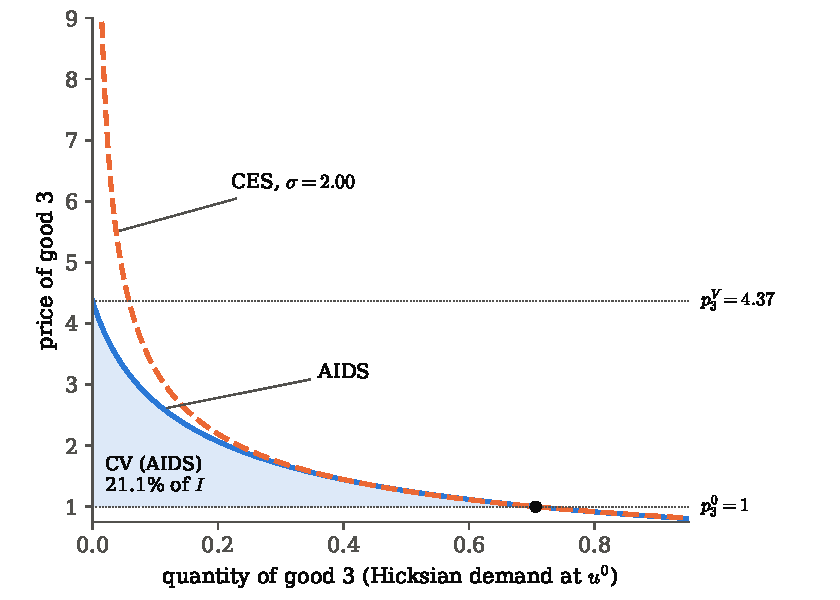
\includegraphics[width=0.78\textwidth]{figures/ch05/virtual_price.pdf}
\caption[Virtual price and the loss from removing a good]{Virtual price and the loss from removing a good.
The solid curve is the AIDS Hicksian demand for good 3 in the running example at the initial utility $u^0$,
with $p_1 = p_2 = 1$. It reaches zero at the virtual price $p_3^V = 4.37$. The shaded area is the compensating
variation of removing good 3, 21.1 percent of income. The dashed curve is the Hicksian demand of a CES system
calibrated to the same share ($0.26$) and own-price elasticity ($-1.738$) at the observed point. It approaches
the price axis only asymptotically, and the area to its left equals 35.2 percent of income. Computed with
\texttt{figures/ch05/src/virtual\_price.py}.}
\label{fig:05-virtual-price}
\end{figure}

\subsection{The extrapolation problem}\label{sec:05-welfare-extrapolation}

\begin{remark}[Virtual prices lie outside the data]\label{rem:05-extrapolation}
Every virtual-price calculation extrapolates. In the running example the virtual price is more than four times
the observed price. In Hausman's cereal data, prices vary by about 50 percent, while the estimated virtual
price is about twice the average price \citep[p.~228]{Hausman1997}. The answer is
then driven by the curvature of the chosen functional form beyond the support of the data. For AIDS the
relevant feature is the shape of shares in log prices, linear when $\beta_i = 0$ and quadratic otherwise.
\Cref{prop:05-variety}(c) shows how sensitive the
result is near unit elasticity: the log virtual price $\frac{1}{-\varepsilon_{ii} - 1}$ explodes as
$\varepsilon_{ii}$ approaches $-1$. \citet{Hausman1997} proposes a lower bound that needs only convexity of
demand: the tangent to the demand curve at the observed price meets the price axis below the true virtual price.
\Cref{ch:newgoods} develops this bound.
\end{remark}

\subsection{Recovering marginal costs from first-order conditions}\label{sec:05-welfare-supply}

Counterfactual prices require marginal costs, which are rarely observed. The standard approach inverts the
firms' pricing conditions, as in \cref{ch:theory} and \cref{ch:diffprod}. We state the conditions in
elasticity form, which is the natural form for product-space demand.

\casehead{Single-product pricing}
A firm that sets the price of product $i$ with constant marginal cost $c_i$ maximizes $(p_i - c_i)q_i(p)$. The
first-order condition is $q_i + (p_i - c_i)\frac{\partial q_i}{\partial p_i} = 0$. Dividing by $q_i$ and
multiplying by $\frac{1}{p_i}$ gives the Lerner condition
$\frac{p_i - c_i}{p_i} = -\frac{1}{\varepsilon_{ii}}$, and solving for the cost gives
\begin{equation}\label{eq:05-foc-single}
  c_i = p_i\Bigl(1 + \frac{1}{\varepsilon_{ii}}\Bigr).
\end{equation}
The condition is meaningful only when $\varepsilon_{ii} < -1$. A profit-maximizing firm never prices on the
inelastic part of its demand. The same condition holds for a product group whose price is set jointly by
perfectly colluding producers, the case used by \citet{ChaudhuriGoldbergJia2006}.

The elasticity in \eqref{eq:05-foc-single} must be \emph{unconditional}. It must include the reallocation of
expenditure across segments and between the category and other goods, computed by the chain rule of
\eqref{eq:05-uncond-elast}. A within-segment elasticity holds segment expenditure fixed. Suppose a segment's
own unconditional elasticity is below $-1$. Raising a brand's price then drains expenditure from the whole
segment, so the unconditional own elasticity is larger in magnitude than the conditional one. Markups computed from
conditional elasticities are then too high. \Cref{tab:05-hlz-own} shows this pattern for all fifteen beer
brands of \cref{sec:05-hlz}.

\casehead{Multiproduct pricing in elasticity form}
Firm $f$ owns the products in $\mathcal{J}_f$ and maximizes $\pi_f = \sum_{k\in\mathcal{J}_f}(p_k - c_k)q_k(p)$.
The first-order condition for $p_j$, $j\in\mathcal{J}_f$, is
\begin{equation*}
  q_j + \sum_{k\in\mathcal{J}_f}(p_k - c_k)\frac{\partial q_k}{\partial p_j} = 0.
\end{equation*}
Let $R_f = \sum_{k\in\mathcal{J}_f}p_kq_k$ be the firm's revenue, $r_k = \frac{p_kq_k}{R_f}$ the revenue share
of product $k$, and $\ell_k = \frac{p_k - c_k}{p_k}$ its Lerner index. Elsewhere the book writes $L$ for the
Lerner index. We write $\ell_k$ in this chapter, where $L$ denotes a likelihood. We multiply the condition by
$\frac{p_j}{R_f}$ and rewrite each term of the sum:
\begin{equation*}
  (p_k - c_k)\frac{\partial q_k}{\partial p_j}\frac{p_j}{R_f}
  = \frac{p_k - c_k}{p_k}\cdot\frac{p_kq_k}{R_f}\cdot\frac{\partial q_k}{\partial p_j}\frac{p_j}{q_k}
  = \ell_k\,r_k\,\varepsilon_{kj}.
\end{equation*}
The first-order conditions become
\begin{equation}\label{eq:05-foc-multi}
  r_j + \sum_{k\in\mathcal{J}_f}\ell_k\,r_k\,\varepsilon_{kj} = 0, \quad j\in\mathcal{J}_f,
  \qquad\text{or}\qquad r_f + E_f^\top m_f = 0.
\end{equation}
Here $r_f$ stacks the revenue shares and $m_f$ has elements $m_k = \ell_kr_k$. The matrix $E_f$ collects the
elasticities among the firm's products, with $(k,j)$ element $\varepsilon_{kj}$. Solving,
\begin{equation}\label{eq:05-markup-multi}
  m_f = -\bigl(E_f^\top\bigr)^{-1}r_f, \qquad \ell_k = \frac{m_k}{r_k}.
\end{equation}
This is the form in \citet[eqs.~7--9 and 14--15]{HausmanLeonardZona1994} and \citet[eqs.~12--15]{Hausman1997},
who write $s$ for the revenue shares and $w$ for $m_f$. The system is homogeneous of degree one in $r_f$, so
the shares can be normalized by any common revenue, such as total market revenue, without changing $\ell$.
Stacking all firms gives a block-diagonal elasticity matrix, one block per firm
\citep[eq.~14]{HausmanLeonardZona1994}.

The elasticity form is equivalent to the matrix markup formula of \cref{ch:diffprod}. Let $\Omega$ be the
ownership matrix and let $D$ have $(j,k)$ element $\frac{\partial q_k}{\partial p_j}$ (note the transposition
relative to the Jacobian of demand). Stacking the first-order conditions of all firms gives
\begin{equation*}
  q + (\Omega\odot D)(p - c) = 0, \qquad\text{so}\qquad p - c = -(\Omega\odot D)^{-1}q.
\end{equation*}
Dividing by market size turns quantities into market shares. Using $\frac{\partial q_k}{\partial p_j} =
\varepsilon_{kj}\frac{q_k}{p_j}$, row $j$ reads $q_j + \sum_k\Omega_{jk}\varepsilon_{kj}\frac{q_k}{p_j}(p_k - c_k) = 0$.
Multiplying by $\frac{p_j}{R_f}$ returns \eqref{eq:05-foc-multi}.

For a firm with two products, \eqref{eq:05-markup-multi} gives
\begin{equation}\label{eq:05-lerner-two}
  \ell_1 = \frac{-\varepsilon_{22} + \frac{r_2}{r_1}\varepsilon_{21}}{\varepsilon_{11}\varepsilon_{22} - \varepsilon_{12}\varepsilon_{21}}.
\end{equation}
With $\varepsilon_{21} = \varepsilon_{12} = 0$ this reduces to $-\frac{1}{\varepsilon_{11}}$. When the two
products are substitutes, the term $\frac{r_2}{r_1}\varepsilon_{21} > 0$ raises the markup on product 1. Part of
the demand lost by raising $p_1$ is recaptured by product 2. The size of the effect depends on the cross
elasticity of the sibling product with respect to $p_1$ and on its relative revenue.

\subsection{Partial identification of marginal cost}\label{sec:05-welfare-bounds}

The first-order condition \eqref{eq:05-foc-single} presumes a model of conduct. In many markets conduct is
unknown, and in regulated markets prices may not satisfy any unconstrained first-order condition.
\citet{ChaudhuriGoldbergJia2006} face both problems in the Indian antibiotics market (\cref{sec:05-cgj}).
Dozens of firms sell each molecule, and many prices are capped by regulation. Their solution is to bound
marginal cost instead of point-identifying it.

\begin{assumption}[Conduct between competition and joint monopoly]\label{ass:05-conduct-order}
For product group $i$ the following hold.
\begin{enumerate}[label=(\roman*)]
  \item Marginal cost $c_i$ is constant.
  \item Group demand $q_i(p_i,p_{-i})$ is differentiable, with $\frac{\partial q_i}{\partial p_i} < 0$.
  \item The group's joint profit $\Pi_i(p_i) = (p_i - c_i)q_i(p_i,p_{-i})$ is strictly quasi-concave in $p_i$,
  with maximizer $p_i^m$.
  \item The observed price satisfies $c_i \le p_i \le p_i^m$.
\end{enumerate}
\end{assumption}

Part (iv) is the substantive assumption. Prices are no lower than marginal cost, and no higher than the price a
joint monopolist of the group would choose given the other prices. Competition within the group and price
caps both move the price into this interval.

\begin{proposition}[Bounds on marginal cost]\label{prop:05-cost-bounds}
Under \cref{ass:05-conduct-order}, $c_i^L \le c_i \le c_i^U$, where
\begin{equation}\label{eq:05-cost-bounds}
  c_i^U = p_i, \qquad c_i^L = p_i\Bigl(1 + \frac{1}{\varepsilon_{ii}(p)}\Bigr),
\end{equation}
and $\varepsilon_{ii}(p)$ is the unconditional own-price elasticity at the observed prices. Equivalently,
$0 \le \ell_i \le -\frac{1}{\varepsilon_{ii}(p)}$.
\end{proposition}

\begin{proof}
The upper bound is the first inequality in part (iv). For the lower bound, a strictly quasi-concave function
increases up to its maximizer. Since $p_i \le p_i^m$, we have
$\Pi_i'(p_i) = q_i + (p_i - c_i)\frac{\partial q_i}{\partial p_i} \ge 0$. Rearranging,
$(p_i - c_i)\bigl(-\frac{\partial q_i}{\partial p_i}\bigr) \le q_i$. Dividing both sides by
$p_i\bigl(-\frac{\partial q_i}{\partial p_i}\bigr) > 0$ gives
\begin{equation*}
  \frac{p_i - c_i}{p_i} \le \frac{q_i}{p_i}\Bigl(-\frac{\partial q_i}{\partial p_i}\Bigr)^{-1} = -\frac{1}{\varepsilon_{ii}}.
\end{equation*}
Solving for $c_i$ gives $c_i \ge p_i\bigl(1 + \frac{1}{\varepsilon_{ii}}\bigr) = c_i^L$.
\end{proof}

These are equations (3.12) and (3.13) of \citet{ChaudhuriGoldbergJia2006}. Several remarks help in using them.
The lower bound is informative only when $\varepsilon_{ii} < -1$. If $-1 < \varepsilon_{ii} < 0$, then
$c_i^L < 0$ and the bound adds nothing to $c_i \ge 0$. The observed price then lies where demand is inelastic,
which no unconstrained joint monopolist would choose. That pattern is itself evidence of competition or
regulation. In the language of \cref{ch:conduct}, the bounds are the endpoints of the conduct-parameter model
$\frac{p_i - c_i}{p_i} = -\frac{\theta}{\varepsilon_{ii}}$ at $\theta = 0$ and $\theta = 1$. The bounds approach
avoids estimating $\theta$, which in a regulated market need not be a stable structural parameter. Bounds are
transparent, and they often suffice for a policy conclusion. In a counterfactual we simulate the outcome at
each bound. The two results bound the counterfactual outcome when that outcome is monotone in marginal cost,
which should be checked in each application.

\subsection{Counterfactual equilibrium after product withdrawal}\label{sec:05-counterfactual}

We now combine virtual prices, cost recovery and the multi-level demand system to simulate the withdrawal of
products. The setting is the two-level system of \cref{sec:05-separability}. An upper level allocates total
expenditure $X$ across segments $G$ with price indices $P_G$, and an AIDS allocates segment expenditure $X_Q$
within segment $Q$. A policy removes the products in $\mathcal{W}\subset Q$, and the products in
$\mathcal{R} = Q\setminus\mathcal{W}$ remain.

\casehead{The equilibrium system}
The unknowns are the virtual prices $p_i^V$ of the withdrawn products, the new prices $p_k'$ of the remaining
products, and the new segment expenditure and price index $X_Q'$ and $P_Q'$. They solve three blocks of
equations.
\begin{enumerate}[label=(S\arabic*)]
  \item Zero shares for withdrawn products. For each $i\in\mathcal{W}$,
  \begin{equation}\label{eq:05-cf-zero}
    0 = \alpha_i + \sum_{j\in\mathcal{W}}\gamma_{ij}\ln p_j^V + \sum_{k\in\mathcal{R}}\gamma_{ik}\ln p_k'
    + \beta_i\ln\frac{X_Q'}{P_Q'}.
  \end{equation}
  \item Pricing of remaining products. For single-product firms or colluding groups,
  \begin{equation}\label{eq:05-cf-price}
    p_k' = c_k\Bigl(1 + \frac{1}{\varepsilon_{kk}(p')}\Bigr)^{-1}, \quad k\in\mathcal{R},
  \end{equation}
  and for multiproduct firms the system \eqref{eq:05-foc-multi} evaluated at the new prices.
  \item Upper-level adjustment. The new index is $P_Q' = \mathbf{P}_Q(p^V_{\mathcal{W}},p'_{\mathcal{R}})$, and
  $X_Q'$ follows from the upper-level share equation of segment $Q$ evaluated at $P_Q'$ and the other segment
  indices.
\end{enumerate}
Equations~\eqref{eq:05-cf-zero} and \eqref{eq:05-cf-price} are equations (3.14) and (3.15) of \citet{ChaudhuriGoldbergJia2006},
written without their market-specific restrictions on the cross-price terms. The elasticities in (S2) are
unconditional and evaluated at the counterfactual prices, including the virtual prices.

One detail of (S2) deserves care. The demand that a remaining firm faces is AIDS demand evaluated at the
virtual prices, and by (S1) those prices move when $p_k'$ moves. For a single withdrawn product $i$, implicit
differentiation of $w_i = 0$ gives
$\frac{\partial\ln p_i^V}{\partial\ln p_j} = -\bigl(\frac{\partial w_i}{\partial\ln p_i}\bigr)^{-1}\frac{\partial w_i}{\partial\ln p_j}$.
The elasticity of demand for product $k$ with respect to $p_j$, once good $i$ has left, is therefore
\begin{equation}\label{eq:05-rationed-elast}
  \varepsilon_{kj}^{-i} = \varepsilon_{kj} - \varepsilon_{ki}\Bigl(\frac{\partial w_i}{\partial\ln p_i}\Bigr)^{-1}\frac{\partial w_i}{\partial\ln p_j},
\end{equation}
with all terms evaluated at $p_i^V$. This is the standard formula for demand under a ration of zero.

\casehead{Solving the system}
A simple algorithm iterates over the blocks. Start at the observed prices and expenditure. Given $p'_{\mathcal{R}}$
and $X_Q'$, solve (S1) for the virtual prices. Update $P_Q'$ and $X_Q'$ with (S3). Update $p'_{\mathcal{R}}$ with
(S2), using elasticities at the current prices. Repeat until the prices stop changing. Newton's method on the
stacked system converges faster when a good starting value is available. Existence and uniqueness are not
guaranteed, so we solve from several starting values and check the second-order conditions. We also verify
that the remaining shares stay positive and that the relevant own elasticities stay below $-1$.

\casehead{Welfare and its decomposition}
Let $E(u,P)$ be the upper-level expenditure function, with $P$ the vector of segment indices. Let $P^0$ be the
observed indices and $P'$ the counterfactual ones, with $P_Q'$ computed from the virtual and new prices. The
compensating variation is \citep[eq.~3.16]{ChaudhuriGoldbergJia2006}
\begin{equation}\label{eq:05-cv-cf}
  CV = E(u^0,P') - E(u^0,P^0).
\end{equation}
To see which mechanism drives it, define two intermediate price vectors. $P^1$ uses virtual prices computed with
$X_Q$ and all remaining prices fixed at their observed values. $P^2$ recomputes the virtual prices letting $X_Q$
respond to the new segment index, still holding the remaining prices fixed. Then
\begin{equation}\label{eq:05-cv-decomp}
  CV = \underbrace{E(u^0,P^1) - E(u^0,P^0)}_{\text{pure variety}}
  + \underbrace{E(u^0,P^2) - E(u^0,P^1)}_{\text{expenditure switching}}
  + \underbrace{E(u^0,P') - E(u^0,P^2)}_{\text{price adjustment}}.
\end{equation}
This is the general form of the decomposition used by \citet{ChaudhuriGoldbergJia2006}. The first term values
the lost products at fixed prices and fixed segment expenditure. The second term exists because the zero-share
condition (S1) is Marshallian. Whenever $\beta_i \neq 0$, the virtual prices depend on segment expenditure, so
they shift once $X_Q$ adjusts. The third term records the repricing of the remaining products. The first two
terms together describe a regime in which price regulation freezes the remaining prices at their old levels.
The decomposition is sequential, so its terms depend on the order in which the changes are introduced.

The welfare of a country adds producer surplus. With $\pi_k = (p_k - c_k)q_k$ computed at the counterfactual
and the observed prices, the change in national welfare is $-CV$ plus the change in the profits of domestic
firms. Profits of foreign firms are excluded from national welfare. They still measure the private gain that
motivates the policy. \Cref{sec:05-cgj-counterfactual} applies this accounting to patents in India.

\begin{example}[Withdrawal in the running example]\label{ex:05-withdrawal}
Treat the running example as a segment with fixed expenditure $X_Q = e$, sold by three single-product firms.
Equation~\eqref{eq:05-foc-single} recovers marginal costs $c = (0.273, 0.406, 0.425)$ from the observed prices and
elasticities. Suppose good 3 is withdrawn. Firms 1 and 2 reprice, facing the demand of consumers who can no
longer buy good 3, with its elasticities given by \eqref{eq:05-rationed-elast}. The new equilibrium has
$p_1' = 1.475$ and $p_2' = 1.365$, increases of 47.5 and 36.5 percent. The own elasticities fall in magnitude
from $-1.375$ and $-1.682$ to $-1.227$ and $-1.423$, because the closest outside option has gone. The total
compensating variation is 71.9 percent of segment expenditure. The pure variety effect, with other prices fixed,
is 21.1 percent (\cref{ex:05-virtual-running}). The price adjustment adds 50.8 percent. Firms 1 and 2 gain
$0.734$ in profit, while firm 3 loses $0.407$. These effects are large because fixing segment expenditure makes
the segment's aggregate demand unit elastic. An upper level with elastic segment demand would add the
expenditure-switching channel and dampen the price response. The computation is in \texttt{virtual\_price.py}.
\end{example}

\section{Case study: Hausman, Leonard and Zona (1994)}\label{sec:05-hlz}

\citet{HausmanLeonardZona1994} (HLZ) built the multi-level AIDS into a tool for antitrust analysis of
differentiated products. They estimated a three-level demand system for beer on store-level scanner data and
identified it with prices of the same brands in other cities. They then used the estimates to predict the price
effects of mergers and to test models of pricing. The paper is short and its data description is thin, but its
method shaped two decades of applied work. We treat it in depth.

\subsection{The economic question}\label{sec:05-hlz-question}

Antitrust questions about consumer goods turn on substitution among brands. Is a set of brands a market? Will
two brands owned by merging firms rise in price? Do observed markups match the predictions of a model of
competition? Each question needs own and cross elasticities for many brands. HLZ argue that the models then in
use restricted these elasticities too much. Representative-consumer models with symmetric preferences and
logit-type models share an \emph{independence of irrelevant alternatives} (IIA) property. Consumers of an
eliminated good spread over the remaining goods in proportion to their market shares. In terms
of elasticities, ``all cross price elasticities with respect to a given good are the same''
\citep[p.~160]{HausmanLeonardZona1994}. HLZ set out to estimate demand without such restrictions.

Store-level scanner data made this possible. Each transaction records units and price paid, by brand and by
stock-keeping unit, and weekly promotions generate large price variation. Two econometric problems remain. The
first is dimensionality. It is ``difficult to conceive of estimating a demand equation with say 135 brands of
cereal or say 40 brands of beer'' (p.~160). The second is identification: at the brand level, cost shifters that
vary across brands and weeks are hard to find. HLZ answer the first problem with multi-stage budgeting and the
second with prices in other cities.

A third theme runs through the applications. Firms in these industries sell many brands. HLZ list Miller High
Life, Miller Lite, Miller Genuine Draft, Milwaukee's Best and Meisterbrau as Miller brands, and note that
Kellogg's produces over 30 cereals (p.~161). A multiproduct firm that raises one brand's price recaptures some
of the lost sales on its other brands. HLZ show how this \emph{cannibalization} changes merger predictions and
tests of conduct.

\subsection{Setting and data}\label{sec:05-hlz-data}

Marketing analysts divide the U.S. beer market into segments: premium, light (low-calorie), imported and
popular-price beer (p.~162). In estimation HLZ use three segments. The premium segment includes imported
beers, which they found belong with premium brands (p.~164). Each segment contains five brands, for fifteen
brands in total (\cref{fig:05-hlz-tree}). The brands include national brands such as Budweiser, Miller and
Coors, Canadian imports such as Molson and Labatts, and regional brands such as Genesee.

\begin{figure}[htbp]
\centering
\begin{tikzpicture}[
  every node/.style={font=\small},
  seg/.style={draw, rounded corners=2pt, minimum width=2.6cm, inner sep=3pt, fill=gray!8},
  brands/.style={align=center, font=\footnotesize, text width=3.3cm}]
  \node[seg, minimum width=3.4cm] (beer) at (0,0) {Beer (top level)};
  \node[seg] (prem) at (-4.6,-1.6) {Premium};
  \node[seg] (pop)  at (0,-1.6)    {Popular price};
  \node[seg] (lig)  at (4.6,-1.6)  {Light};
  \foreach \s in {prem,pop,lig} \draw[-{Latex[length=2mm]}] (beer.south) -- (\s.north);
  \node[brands, anchor=north] (b1) at (-4.6,-2.2) {Budweiser\\ Molson\\ Labatts\\ Miller\\ Coors};
  \node[brands, anchor=north] (b2) at (0,-2.2) {Old Milwaukee\\ Genesee\\ Milwaukee's Best\\ Busch\\ Piels Lager};
  \node[brands, anchor=north] (b3) at (4.6,-2.2) {Genesee Light\\ Coors Light\\ Old Milwaukee Light\\ Lite\\ Molson Light};
  \foreach \s/\b in {prem/b1,pop/b2,lig/b3} \draw[-{Latex[length=2mm]}] (\s.south) -- (\b.north);
  \node[anchor=west, font=\footnotesize\itshape] at (6.6,0) {top};
  \node[anchor=west, font=\footnotesize\itshape] at (6.6,-1.6) {middle};
  \node[anchor=west, font=\footnotesize\itshape] at (6.6,-3.2) {bottom};
\end{tikzpicture}
\caption[The three-level budgeting tree of Hausman, Leonard and Zona]{The three-level budgeting tree of
\citet{HausmanLeonardZona1994}. The top level determines beer consumption relative to other goods, the middle
level allocates beer expenditure across three segments, and the bottom level allocates each segment's
expenditure across five brands. Imported beers are included in the premium segment. Brand lists from HLZ,
Tables 2 to 5.}
\label{fig:05-hlz-tree}
\end{figure}

The data are cash-register records from individual stores, aggregated to the metropolitan area (SMSA) level.
For each brand they give sales and price per unit, after aggregating over container sizes (p.~160). Most price
variation comes from supermarket chains running low-price promotions on a brand in a given week (p.~167).
In most cases manufacturers sell at wholesale nationally, with a uniform wholesale price (p.~161), which
motivates the
identification strategy below. The paper reports little else about the sample. Two graphs show weekly sales of
Budweiser and Genesee in Buffalo in February and March 1988 and in March to June 1990. The middle-level
regressions of Table 1 use 101 observations. HLZ do not report the list of cities, the sample period or the
number of stores. The top level uses national monthly data from the Bureau of Labor Statistics covering
sixteen years (p.~164). The share equations also include a time trend and the log number of stores.

\subsection{The three-level demand model}\label{sec:05-hlz-model}

HLZ apply the multi-stage budgeting framework of \cref{sec:05-separability} with three levels. We write their
equations in this chapter's notation. Cities are indexed by $n = 1,\dots,N$ (in this section $N$ counts cities)
and weeks by $t$. Segments are $G$ and $H$, and brands are $i$ and $j$.

\casehead{Bottom level: brands within a segment}
For brand $i$ in segment $G$,
\begin{equation}\label{eq:05-hlz-bottom}
  w_{int} = \alpha_{in} + \beta_i\ln\frac{X_{Gnt}}{P_{Gnt}} + \sum_{j\in G}\gamma_{ij}\ln p_{jnt} + \xi_{int}.
\end{equation}
This is equation (1) of \citet{HausmanLeonardZona1994}. Here $w_{int}$ is the revenue share of brand $i$ in segment expenditure
$X_{Gnt}$, $P_{Gnt}$ is a segment price index and $p_{jnt}$ is the price of brand $j$. The intercept
$\alpha_{in}$ is a brand-city effect. This is an AIDS for the segment, with symmetry
$\gamma_{ij} = \gamma_{ji}$ imposed in estimation. The $\gamma_{ij}$ are free within the segment, so no IIA-type
restriction constrains the cross elasticities among the brands that compete most closely. A test of
$\beta_i = 0$ is a test of segment homotheticity. HLZ stress that the expenditure variable must be segment
expenditure (p.~163), in the words that \citet{Hausman1997} repeats and that we quoted in
\cref{sec:05-second-stage}.

\casehead{Middle level: segments}
Given the bottom-level estimates, HLZ construct a price index for each segment. They use either the exact index
implied by the bottom-level expenditure function or a weighted-average index of the Laspeyres type, and report
that the choice matters little (p.~164). The segment demands are log-log:
\begin{equation}\label{eq:05-hlz-middle}
  \ln q_{Gnt} = \alpha_{Gn} + \beta_G\ln X_{Bnt} + \sum_{H}\vartheta_{GH}\ln P_{Hnt} + \xi_{Gnt},
\end{equation}
where $q_{Gnt}$ is the quantity of segment $G$ and $X_{Bnt}$ is total beer expenditure (HLZ eq.~2, where
the price coefficients are written $\delta_k$). Because beer expenditure is held fixed, $\beta_G$ and
$\vartheta_{GH}$ are conditional elasticities. Slutsky restrictions are not imposed at this level (fn.~3).
Exact two-stage budgeting under Gorman's results, discussed in \citet{BlackorbyPrimontRussell1978}, requires
additive separability at the level above. HLZ note
that AIDS is a generalized Gorman polar form, so Gorman's theorem applies, and that a less restrictive middle
level, not consistent with exact two-stage budgeting, gives similar results (fn.~2).

\casehead{Top level: beer}
Overall beer consumption $Q_{Bt}$ is
\begin{equation}\label{eq:05-hlz-top}
  \ln Q_{Bt} = \varphi_0 + \varphi_1\ln y_t + \varphi_2\ln P_{Bt} + Z_t^\top\psi + \xi_{Bt}.
\end{equation}
This is HLZ's equation (3). Here $y_t$ is deflated disposable income and $P_{Bt}$ is the deflated beer price index. The vector
$Z_t$ holds demographics, monthly seasonal factors and the minimum legal age for buying beer. The coefficient
$\varphi_2$ is the overall price elasticity of beer. HLZ estimate it by instrumental variables on the national
monthly data, with cost shifters for ingredients, packaging and labor as instruments.

\casehead{From three levels to unconditional elasticities}
Estimation runs bottom-up, and the elasticities that matter for competition combine all three levels. The
two-level chain rule of \eqref{eq:05-uncond-elast} extends directly. Take brand $i$ in segment $G$ and brand $j$
in segment $H$, and drop the city and week subscripts. Let $\varepsilon_{ij}\big|_{X_G}$ be the
within-segment elasticity at fixed segment expenditure and $\eta_{i\mid G} = 1 + \frac{\beta_i}{w_i}$ the
elasticity of brand $i$ with respect to segment expenditure. Then
\begin{equation*}
  \varepsilon_{ij} = \indic(G = H)\,\varepsilon_{ij}\big|_{X_G} + \eta_{i\mid G}\,\frac{\partial\ln X_G}{\partial\ln p_j}.
\end{equation*}
Segment expenditure is $X_G = P_Gq_G$, so $\ln X_G = \ln P_G + \ln q_G$. The index $P_G$ responds to $p_j$ only
if $H = G$. The quantity $q_G$ responds through the price index $P_H$ and through beer expenditure:
\begin{equation*}
  \frac{\partial\ln q_G}{\partial\ln p_j} = \Bigl[\vartheta_{GH} + \beta_G\frac{\partial\ln X_B}{\partial\ln P_H}\Bigr]\frac{\partial\ln P_H}{\partial\ln p_j}.
\end{equation*}
Beer expenditure is $X_B = P_BQ_B$, and with income fixed the top level gives
$\frac{\partial\ln X_B}{\partial\ln P_B} = 1 + \varphi_2$. If the beer index has segment weights $w_H$ (the shares
of the segments in beer expenditure), then $\frac{\partial\ln P_B}{\partial\ln P_H} = w_H$. Collecting terms,
\begin{equation}\label{eq:05-hlz-uncond}
  \varepsilon_{ij} = \indic(G = H)\,\varepsilon_{ij}\big|_{X_G}
  + \eta_{i\mid G}\Bigl[\indic(G = H) + \vartheta_{GH} + \beta_G(1 + \varphi_2)w_H\Bigr]\frac{\partial\ln P_H}{\partial\ln p_j}.
\end{equation}
For a Stone or Laspeyres segment index, $\frac{\partial\ln P_H}{\partial\ln p_j}$ is the weight of brand $j$ in
the index. For the exact translog index it equals $w_j - \beta_j\ln\frac{X_H}{P_H}$ (\cref{sec:05-aids}).

Equation~\eqref{eq:05-hlz-uncond} has two consequences. For the own elasticity ($j = i$), the bracket equals
$1 + \vartheta_{GG} + \beta_G(1 + \varphi_2)w_G$. It is negative whenever the segment's own conditional
elasticity is well below $-1$, as it is in the beer data. The unconditional own elasticity is then larger in
magnitude than the conditional one. For brands in different segments, $\varepsilon_{ij}$ depends on brand $j$
only through its weight in index $H$, and on brand $i$ only through $\eta_{i\mid G}$. All brand-pair specific
substitution across segments is ruled out. This is the price of the dimension reduction.

The restriction has a compensated counterpart. By the theorem of \citet{GoldmanUzawa1964}
(\cref{prop:05-goldman-uzawa}), weak separability implies $S_{ij} = \mu_{GH}\frac{\partial q_i}{\partial I}\frac{\partial q_j}{\partial I}$
for $i\in G$, $j\in H$, $G\neq H$. To convert to elasticities, we use
$\frac{\partial q_i}{\partial I} = \frac{\partial q_i}{\partial X_G}\frac{\partial X_G}{\partial I}
= \eta_{i\mid G}\frac{q_i}{X_G}\frac{\partial X_G}{\partial I}$ and the same expression for good $j$ in segment $H$.
Then
\begin{equation*}
  \varepsilon^h_{ij} = \frac{p_j}{q_i}S_{ij}
  = \mu_{GH}\,\eta_{i\mid G}\,\eta_{j\mid H}\,\frac{\partial X_G}{\partial I}\frac{\partial X_H}{\partial I}\,
    \frac{p_jq_j}{X_GX_H},
\end{equation*}
which gives
\begin{equation*}
  \varepsilon^h_{ij} = \lambda_{GH}\,w_{j\mid H}\,\eta_{i\mid G}\,\eta_{j\mid H},
  \qquad \lambda_{GH} = \frac{\mu_{GH}}{X_G}\frac{\partial X_G}{\partial I}\frac{\partial X_H}{\partial I},
\end{equation*}
where $w_{j\mid H}$ is the share of brand $j$ in segment $H$ and $\lambda_{GH}$ depends only on the pair of
segments. HLZ state the restriction as $\varepsilon^h_{ij} = \lambda_{GH}\eta_{i\mid G}\eta_{j\mid H}$
\citep[eq.~5]{HausmanLeonardZona1994}. The exact conversion adds the within-segment share of brand $j$. Either
way, a segment-pair constant and brand-level expenditure elasticities determine all compensated substitution
across segments.

The dimension reduction is large. A complete AIDS for fifteen brands has $\frac{15 \times 14}{2} = 105$ free
price coefficients after symmetry and homogeneity. Three five-brand segments have $3 \times 10 = 30$, the middle
level adds nine segment price elasticities, and the top level adds one.

\subsection{Identification with prices in other cities}\label{sec:05-hlz-identification}

Prices in \eqref{eq:05-hlz-bottom} are endogenous if retailers and manufacturers set them knowing local demand
conditions. Cost shifters that vary by brand and week are rarely available. An ``insufficient number of input
prices may exist or they may not be reported with high enough frequency'' (p.~164). HLZ exploit the panel
structure of the data instead. They model the price of brand $j$ in city $n$ and week $t$ as
\begin{equation}\label{eq:05-hlz-price}
  \ln p_{jnt} = \rho_j\ln c_{jt} + \mu_{jn} + \zeta_{jnt}.
\end{equation}
This is HLZ's equation (4), with our $\rho_j$, $\mu_{jn}$ and $\zeta_{jnt}$ in place of their $\delta_j$,
$\alpha_{jn}$ and $w_{jnt}$. Here $c_{jt}$ is the cost of brand $j$, assumed to have no
city-specific time variation, consistent with national shipments and advertising. The term $\mu_{jn}$ is a
city-brand differential reflecting transport costs or local wages. The shock $\zeta_{jnt}$ has mean zero and
captures local promotions.

\begin{assumption}[Prices in other cities as instruments]\label{ass:05-hausman-iv}
In \eqref{eq:05-hlz-price} the following hold.
\begin{enumerate}[label=(\roman*)]
  \item The cost component $c_{jt}$ is common to all cities.
  \item The city-brand effects $\mu_{jn}$ are constant over time.
  \item The local shocks $\zeta_{jnt}$ are independent across cities. They may be correlated across brands
  within a city \citep[fn.~19]{Hausman1997}.
  \item The demand errors $\xi_{int}$ are uncorrelated with the cost component and with the local price shocks
  of other cities.
\end{enumerate}
\end{assumption}

Let a tilde denote the deviation from the city-brand mean, the within transformation that removes $\mu_{jn}$
and the fixed effects in \eqref{eq:05-hlz-bottom}. Under \cref{ass:05-hausman-iv} the prices of every brand of
the segment in any other city $n'\neq n$ satisfy the moment conditions
\begin{equation}\label{eq:05-hausman-iv}
  \E\bigl[\tilde\xi_{int}\,\widetilde{\ln p}_{jn't}\bigr] = 0, \qquad j\in G,\ n'\neq n.
\end{equation}
Instruments of this kind are now called \emph{Hausman instruments}. Relevance and exclusion follow from
\eqref{eq:05-hlz-price}. The price in city $n'$ shares the cost component with the price in city $n$, while the
local shocks are independent, so
\begin{equation*}
  \Cov\bigl(\widetilde{\ln p}_{jn't},\widetilde{\ln p}_{jnt}\bigr) = \rho_j^2\Var\bigl(\widetilde{\ln c}_{jt}\bigr) > 0
\end{equation*}
whenever national costs vary over time. The covariance with the demand error is
\begin{equation*}
  \Cov\bigl(\widetilde{\ln p}_{jn't},\tilde\xi_{int}\bigr)
  = \rho_j\Cov\bigl(\widetilde{\ln c}_{jt},\tilde\xi_{int}\bigr) + \Cov\bigl(\tilde\zeta_{jn't},\tilde\xi_{int}\bigr),
\end{equation*}
and both terms are zero by part (iv). In words, ``prices in one city (after elimination of city and brand specific effects)
are driven by underlying costs'' (p.~165).

The first stage regresses $\ln p_{jnt}$ on the brand-city effects, the exogenous regressors and the prices of the
segment's brands in other cities, either city by city or averaged. With more than two cities the model is
overidentified, and HLZ point to the tests of \citet{HausmanTaylor1981} for checking the instrument assumptions
(fn.~4). The logic is that of \citet{HausmanTaylor1981}: after unit effects are removed, variation shared with
other units serves as an instrument. The share equations are estimated as a system, as the residual covariance
matrices reported with Tables 2 to 4 suggest, and symmetry is imposed across equations.

HLZ also offer a second interpretation. Suppose supermarkets set weekly prices under constant short-run marginal
cost and do not adjust them to clear the market. Prices are then predetermined with respect to the demand errors,
and ordinary least squares is consistent. Segment expenditure $X_{Gnt}$ may still need instruments, since it
responds to the same demand shocks. The choice between the two views can be tested with the specification test
of \citet{Hausman1978}. That test compares the IV and OLS estimates through
\begin{equation*}
  \mathcal{H} = (\hat b_{IV} - \hat b_{OLS})^\top\bigl[\widehat{\Var}(\hat b_{IV}) - \widehat{\Var}(\hat b_{OLS})\bigr]^{-1}(\hat b_{IV} - \hat b_{OLS}),
\end{equation*}
which is asymptotically chi-squared under exogeneity, with degrees of freedom equal to the number of
coefficients tested. HLZ describe the test but do not report its outcome for beer.

Later work adopted these instruments widely. \citet{Nevo2001} uses regional quarterly average prices of the same
brand, excluding the city being instrumented, in his study of breakfast cereals. \Cref{ch:logit} and
\cref{ch:blp} return to them.

\subsection{Validity: Bresnahan's critique}\label{sec:05-bresnahan-critique}

The identifying assumption rules out demand shocks that are common across cities and reflected in prices.
\citet{Bresnahan1997} made this objection in his comment on \citet{Hausman1997}, which uses the same strategy for
cereals. For the assumption to hold, ``there can be no successful nationwide advertising campaigns which shift
the demand for individual brands or products'' \citep[p.~241]{Bresnahan1997}. There can be no national fads and
no slow national acceptance of new brands. Adding advertising to the demand equation does not settle the issue,
because the econometrician does not observe which campaigns succeed (fn.~6). The fallback that prices are
predetermined requires such shocks to be unforeseen when prices are set, which Bresnahan finds unlikely for
national campaigns. If national shocks exist and supply slopes up, prices in other cities move with the demand
error. Supply can slope up in the one-week run because inventories cannot adjust or because of market power
(fn.~7).

\casehead{The bias with one product}
We derive the bias in the simplest version of Bresnahan's model: one product, linear demand, single-product
Bertrand pricing and constant marginal cost. In city $n$ and week $t$,
\begin{equation*}
  q_{nt} = d + a\,p_{nt} + \xi_{nt}, \quad a < 0, \qquad\qquad p_{nt} = c_{nt} + \frac{q_{nt}}{-a}.
\end{equation*}
The pricing equation is the first-order condition $q + (p - c)a = 0$. Substituting demand into it gives
$p = c - \frac{d}{a} - p - \frac{\xi}{a}$, so
\begin{equation*}
  p_{nt} = \frac{1}{2}c_{nt} - \frac{d + \xi_{nt}}{2a}.
\end{equation*}
Let the demand error have a national and a local part, $\xi_{nt} = \chi_t + e_{nt}$, and let cost have the same
structure, $c_{nt} = \bar c_t + v_{nt}$. The national components have variances $\sigma_\chi^2$ and $\sigma_c^2$.
All components are mutually independent, and the local ones are independent across cities. The instrument for
$p_{nt}$ is $p_{n't}$ with $n'\neq n$. Only the national components survive in the covariances:
\begin{equation*}
  \Cov(p_{n't},\xi_{nt}) = -\frac{\sigma_\chi^2}{2a}, \qquad
  \Cov(p_{n't},p_{nt}) = \frac{\sigma_c^2}{4} + \frac{\sigma_\chi^2}{4a^2}.
\end{equation*}
The IV estimator therefore converges to
\begin{equation}\label{eq:05-iv-bias-scalar}
  \plim\hat a = a + \frac{\Cov(p_{n't},\xi_{nt})}{\Cov(p_{n't},p_{nt})}
  = a - \frac{2a\,\sigma_\chi^2}{a^2\sigma_c^2 + \sigma_\chi^2} = a(1 - 2\lambda),
  \qquad \lambda = \frac{\sigma_\chi^2}{a^2\sigma_c^2 + \sigma_\chi^2}.
\end{equation}
The weight $\lambda\in[0,1]$ is the share of national demand shocks in the price variation common to all
cities. Without national demand shocks ($\lambda = 0$) the estimator is consistent. Otherwise the estimate lies
between $a$ and $-a$, biased toward zero, so demand looks too steep. When $\lambda > \frac{1}{2}$ the estimated
slope even has the wrong sign. At $\lambda = 1$ the estimator recovers $-a$, the slope of the supply relation
$q = -a(p - c)$. In Bresnahan's words, the estimator then behaves ``like doing ordinary least squares on a supply
and demand system'' (p.~242).

\casehead{The bias with many products}
The same logic extends to $J$ products, and the exact bias has a compact form. Let demand be
$q_{nt} = d + A\,p_{nt} + \xi_{nt}$, with $A = [a_{jk}]$ and $a_{jk} = \frac{\partial q_j}{\partial p_k}$. Single-product
Bertrand pricing gives $p_{jnt} = c_{jnt} + \frac{q_{jnt}}{-a_{jj}}$, or $p = c + \Theta^{-1}q$ with
$\Theta = \diag(-a_{11},\dots,-a_{JJ})$. Multiplying by $\Theta$ and substituting demand,
\begin{equation*}
  \Theta p_{nt} = \Theta c_{nt} + d + Ap_{nt} + \xi_{nt}, \qquad\text{so}\qquad p_{nt} = (\Theta - A)^{-1}\bigl(d + \Theta c_{nt} + \xi_{nt}\bigr).
\end{equation*}
This is the price system in the appendix of \citet{Bresnahan1997}. Let the national demand and cost components
have covariance matrices $\Sigma_\chi$ and $\Sigma_c$, and write $M = (\Theta - A)^{-1}$. Equation $j$ is estimated
by IV with the vector of other-city prices $p_{n't}$ as instruments. Its coefficient vector, the transpose of
row $j$ of $A$, converges to $A_{j\cdot}^\top + [\E(\tilde p_{n't}\tilde p_{nt}^\top)]^{-1}\E(\tilde p_{n't}\xi_{jnt})$.
The two moments are
\begin{equation*}
  \E(\tilde p_{n't}\tilde p_{nt}^\top) = M\bigl(\Theta\Sigma_c\Theta + \Sigma_\chi\bigr)M^\top, \qquad
  \E(\tilde p_{n't}\xi_{jnt}) = M\Sigma_\chi\mathbf{e}_j,
\end{equation*}
where $\mathbf{e}_j$ is the $j$th unit vector. The bias of equation $j$ is therefore
$(\Theta - A)^\top(\Theta\Sigma_c\Theta + \Sigma_\chi)^{-1}\Sigma_\chi\mathbf{e}_j$. Stacking the equations and using the symmetry of
the covariance matrices gives the following result.

\begin{proposition}[Bias of other-city price instruments]\label{prop:05-iv-bias}
In the linear model above, IV estimation with other-city prices satisfies
\begin{equation}\label{eq:05-iv-bias}
  \plim\hat A = (I - \Lambda)A + \Lambda\Theta, \qquad \Lambda = \Sigma_\chi\bigl(\Theta\Sigma_c\Theta + \Sigma_\chi\bigr)^{-1}.
\end{equation}
The estimate is a matrix-weighted average of the demand slopes $A$ and the supply slopes $\Theta$. With
$\Sigma_\chi = 0$ it is consistent, and with $\Sigma_c = 0$ it recovers $\Theta$, which has own slopes $-a_{jj}$ and
zero cross slopes.
\end{proposition}

When the national demand and cost shocks are uncorrelated across products, $\Lambda = \diag(\lambda_1,\dots,\lambda_J)$ with
$\lambda_j = \frac{\sigma_{\chi j}^2}{a_{jj}^2\sigma_{cj}^2 + \sigma_{\chi j}^2}$. Then
$\plim\hat a_{jj} = (1 - 2\lambda_j)a_{jj}$ and $\plim\hat a_{jk} = (1 - \lambda_j)a_{jk}$. Own slopes are biased
toward zero as in the one-product case, and cross slopes are attenuated toward zero. Correlated national shocks
change the cross terms. The bias of $a_{12}$ is $-\Lambda_{11}a_{12} - 2\Lambda_{12}a_{22}$, and the second term is
positive when $\Lambda_{12} > 0$. Cross slopes can then be inflated. \texttt{bresnahan\_bias\_check.py} confirms
\eqref{eq:05-iv-bias} by simulation. For example, with $A = \bigl[\begin{smallmatrix}-2 & 0.5\\ 0.5 & -1.5\end{smallmatrix}\bigr]$,
$\Sigma_c = 0.3I$ and $\Sigma_\chi = 0.4I$, the probability limit is
$\bigl[\begin{smallmatrix}-1.00 & 0.375\\ 0.314 & -0.384\end{smallmatrix}\bigr]$. If the national shocks have
correlation $0.8$ across the two products, it becomes
$\bigl[\begin{smallmatrix}-1.31 & 1.11\\ 0.87 & -0.57\end{smallmatrix}\bigr]$.

\casehead{Bresnahan's printed result}
Bresnahan states that the sign and magnitude of the bias are governed by $\Sigma_\chi[\diag(-\gamma) - \gamma]^{-1}$,
in his notation $\gamma_{jk} = a_{jk}$. This matrix is the covariance between other-city prices and demand
errors, $M\Sigma_\chi$ up to transposition. For two products whose national shocks have correlation $\varrho$, his
appendix (pp.~246--247) reports the elements
\begin{equation*}
  \frac{\sigma}{4\gamma_{11}\gamma_{22} - \gamma_{12}\gamma_{21}}
  \begin{bmatrix} -2\gamma_{22} + \varrho\gamma_{21} & \gamma_{12} - 2\varrho\gamma_{11}\\
  -2\varrho\gamma_{22} + \gamma_{21} & \varrho\gamma_{12} - 2\gamma_{11}\end{bmatrix}.
\end{equation*}
He concludes that the on-diagonal bias has the sign of
$-2\gamma_{22} + \varrho\gamma_{12}$ and the off-diagonal bias the sign of $\gamma_{12} - 2\varrho\gamma_{11}$. At
$\varrho = 0$ these are positive: own coefficients are biased toward zero and cross coefficients away from zero.
The printed algebra has typographical slips. The intermediate inverse has the wrong signs off the diagonal,
although the final matrix is correct, and the text writes $\varrho\gamma_{12}$ where the matrix has
$\varrho\gamma_{21}$, which coincide under symmetry. The reading of covariance signs as bias signs is exact with
one price. With several endogenous prices the bias also involves the inverse of the first-stage covariance
matrix, as \eqref{eq:05-iv-bias} shows. With $\varrho = 0$ the cross coefficients are attenuated, while
sufficiently correlated national shocks inflate them. Bresnahan's footnote 9 already hedges the cross-price
claim, saying that it ``depends on the covariances of the shocks to demand across products.'' Correlated
national shocks can also bias an own slope away from zero. The bias of $a_{jj}$ is the diagonal element
$2\Lambda_{jj}|a_{jj}| - \sum_{k\neq j}\Lambda_{jk}a_{kj}$ of $\Lambda(\Theta - A)$, and the second term can dominate.
With the matrix $A$ above, $\Sigma_c = \diag(5, 0.01)$ and
$\Sigma_\chi = 0.4\bigl[\begin{smallmatrix}1 & 0.95\\ 0.95 & 1\end{smallmatrix}\bigr]$ give
$\plim\hat a_{11} = -2.44$, farther from zero than the true $-2$. The own-price bias toward zero holds when
$2\Lambda_{jj}|a_{jj}| > \sum_{k\neq j}\Lambda_{jk}a_{kj}$, for example when national demand and cost shocks are
uncorrelated across products.

\casehead{What the critique implies}
National demand shocks typically make estimated own elasticities too small in magnitude. Markups recovered from
\eqref{eq:05-foc-multi} are then too high, simulated merger price increases too large, and the value of new goods
too large. Bresnahan's own concern was the last of these. \citet[fn.~25]{Hausman1997} anticipates the objection
by citing the beer estimates of HLZ, whose own-price elasticities lie ``in the range of about $-4.0$ to $-6.2$''.
He concludes that the method does not mechanically produce small elasticities. The reply is incomplete. A bias
toward zero is compatible with large estimates if the true elasticities are larger still. The assumption can be
probed in the data. Overidentification tests across cities are one check. A more direct symptom of national
shocks is correlation between the demand residuals of the same brand in different cities in the same week.
Instruments based on observed local cost variation offer a comparison, as in \citet{Nevo2001}. Bresnahan
himself points to other approaches to estimating substitution, including the then recent method of
\citet{Berry1994} (fn.~10). The critique
applies to every use of Hausman instruments, including random-coefficient models (\cref{ch:blp}).

\subsection{Results}\label{sec:05-hlz-results}

\casehead{Top and middle levels}
The overall price elasticity of beer is $-1.36$, with standard error 0.21 (p.~164). \Cref{tab:05-hlz-table1}
reproduces the segment equations. Each column is a segment demand equation, and because the equations are
log-log, the coefficients are conditional elasticities. Expenditure elasticities are close to one. The own
price elasticities are about $-2.7$ for premium and popular-price beer and $-2.4$ for light beer. These are large
for segment-level elasticities. They imply that a hypothetical attempt to raise all premium prices would not pay
if light and popular prices stayed put (p.~166).

\begin{table}[htbp]
\centering
\caption{Segment demand equations for beer}\label{tab:05-hlz-table1}
\begin{threeparttable}
\begin{tabular}{@{}lccc@{}}
\toprule
 & Premium & Popular & Light \\
\midrule
Constant & $0.501$ & $-4.021$ & $-1.183$ \\
 & $(0.283)$ & $(0.560)$ & $(0.377)$ \\
$\ln$ beer expenditure & $0.978$ & $0.943$ & $1.067$ \\
 & $(0.011)$ & $(0.022)$ & $(0.015)$ \\
$\ln P_{\text{premium}}$ & $-2.671$ & $2.704$ & $0.424$ \\
 & $(0.123)$ & $(0.244)$ & $(0.166)$ \\
$\ln P_{\text{popular}}$ & $0.510$ & $-2.707$ & $0.747$ \\
 & $(0.097)$ & $(0.193)$ & $(0.127)$ \\
$\ln P_{\text{light}}$ & $0.701$ & $0.518$ & $-2.424$ \\
 & $(0.070)$ & $(0.140)$ & $(0.092)$ \\
Time & $-0.001$ & $-0.000$ & $0.002$ \\
 & $(0.000)$ & $(0.001)$ & $(0.000)$ \\
$\ln$ number of stores & $-0.035$ & $0.253$ & $-0.176$ \\
 & $(0.016)$ & $(0.034)$ & $(0.023)$ \\
\midrule
Observations & \multicolumn{3}{c}{101} \\
\bottomrule
\end{tabular}
\begin{tablenotes}[flushleft]\footnotesize
\item Notes: Dependent variable is the log quantity of the segment, \eqref{eq:05-hlz-middle}. Each column is one
equation. Coefficients on log prices are elasticities conditional on beer expenditure. Standard errors in
parentheses. Source: \citet[Table 1]{HausmanLeonardZona1994}.
\end{tablenotes}
\end{threeparttable}
\end{table}

The cross elasticities are large and positive. A 10 percent rise in the premium price index raises light-beer
demand by about 4.2 percent, and the popular-price equation has a coefficient of 2.70 on the premium index. HLZ
draw an antitrust conclusion. Claims that segments such as light and popular beer form separate markets are
contradicted by the data, because enough marginal consumers switch segments in response to price (p.~166).

\casehead{Bottom level}
\Cref{tab:05-hlz-table2} reproduces the premium-segment share equations. The AIDS coefficients are not
elasticities, so HLZ report the implied conditional own-price elasticities in the last row. Premium brands have
conditional own elasticities between $-3.5$ and $-5.0$. The conditional cross elasticities of Budweiser lie
between 0.4 and 1.0, and Coors has a conditional cross elasticity of 1.0 with respect to Labatts (p.~166). The
coefficients on $\ln\frac{X}{P}$ are small. HLZ describe income effects at the bottom level as very small
(p.~169).

\begin{table}[htbp]
\centering
\caption{Brand share equations, premium segment}\label{tab:05-hlz-table2}
\begin{threeparttable}
\begin{tabular}{@{}lccccc@{}}
\toprule
 & Budweiser & Molson & Labatts & Miller & Coors \\
\midrule
Constant & $0.393$ & $0.377$ & $0.230$ & $-0.104$ & \\
 & $(0.062)$ & $(0.078)$ & $(0.056)$ & $(0.031)$ & \\
Time & $0.001$ & $-0.000$ & $0.001$ & $0.000$ & \\
 & $(0.000)$ & $(0.000)$ & $(0.000)$ & $(0.000)$ & \\
$\ln\frac{X}{P}$ & $-0.004$ & $-0.011$ & $-0.006$ & $0.017$ & \\
 & $(0.006)$ & $(0.007)$ & $(0.005)$ & $(0.003)$ & \\
$\ln p_{\text{Budweiser}}$ & $-0.936$ & $0.372$ & $0.243$ & $0.150$ & \\
 & $(0.041)$ & $(0.231)$ & $(0.034)$ & $(0.018)$ & \\
$\ln p_{\text{Molson}}$ & $0.372$ & $-0.804$ & $0.183$ & $0.130$ & \\
 & $(0.231)$ & $(0.031)$ & $(0.022)$ & $(0.012)$ & \\
$\ln p_{\text{Labatts}}$ & $0.243$ & $0.183$ & $-0.588$ & $0.028$ & \\
 & $(0.034)$ & $(0.022)$ & $(0.044)$ & $(0.019)$ & \\
$\ln p_{\text{Miller}}$ & $0.150$ & $0.130$ & $0.028$ & $-0.377$ & \\
 & $(0.018)$ & $(0.012)$ & $(0.019)$ & $(0.017)$ & \\
$\ln$ number of stores & $-0.010$ & $0.005$ & $-0.036$ & $0.022$ & \\
 & $(0.009)$ & $(0.012)$ & $(0.008)$ & $(0.005)$ & \\
\midrule
Conditional own-price elasticity & $-3.527$ & $-5.049$ & $-4.277$ & $-4.201$ & $-4.641$ \\
 & $(0.113)$ & $(0.152)$ & $(0.245)$ & $(0.147)$ & $(0.203)$ \\
\bottomrule
\end{tabular}
\begin{tablenotes}[flushleft]\footnotesize
\item Notes: Each column is the share equation \eqref{eq:05-hlz-bottom} of one brand. Symmetry is imposed in
estimation. The Coors equation and the coefficients on the Coors price are not reported. The residual covariance
matrix reported by HLZ is omitted. Standard errors in parentheses. The coefficient linking the Budweiser and Molson
prices is reported with standard error 0.231 in both places. HLZ do not report the number of observations for
the brand equations. Source: \citet[Table 2]{HausmanLeonardZona1994}.
\end{tablenotes}
\end{threeparttable}
\end{table}

\begin{example}[Reading an AIDS table]\label{ex:05-hlz-reading}
The AIDS formulas of \cref{sec:05-aids} let us recover more from \cref{tab:05-hlz-table2} than HLZ report.
Ignoring the small expenditure terms, the conditional elasticities are
$\varepsilon_{ij} \approx -\indic(i = j) + \frac{\gamma_{ij}}{w_i}$. Inverting the own elasticity gives the
within-segment share implied by the table, $w_i = \frac{\gamma_{ii}}{\varepsilon_{ii} + 1}$. For Budweiser,
$w_1 = \frac{-0.936}{-2.527} = 0.370$. The same calculation gives 0.199 for Molson, 0.179 for Labatts and 0.118 for
Miller, which leaves 0.134 for Coors. The omitted Coors price can be recovered from homogeneity,
$\gamma_{i5} = -\sum_{j\le 4}\gamma_{ij}$, which gives $(0.171, 0.119, 0.134, 0.069)$. Adding up then gives
$\gamma_{55} = -0.493$. The implied Coors own elasticity is $-1 + \frac{-0.493}{0.134} = -4.68$, close to the
reported $-4.641$. The cross elasticities of Coors with respect to Budweiser, Molson, Labatts and Miller are
$\frac{\gamma_{5j}}{w_5} = 1.28$, $0.89$, $1.00$ and $0.52$. HLZ report 1.25, 0.86, 1.0 and 0.52 in the text
(pp.~166 and 168). The Budweiser row gives cross elasticities from 0.40 to 1.00, matching the range HLZ quote.
These are our calculations (\texttt{hlz\_table2\_check.py}). They suggest that homogeneity was imposed with the
Coors price as the omitted one, and they show how much an AIDS table reveals once the shares are known.
\end{example}

\Cref{tab:05-hlz-own} collects the conditional own elasticities of all fifteen brands from HLZ's Tables 2 to 4 and
the unconditional (overall) own elasticities of their Table 5. HLZ find somewhat higher own elasticities for
popular-price brands than for premium or light brands, which they read as lower brand loyalty (pp.~167 and 169). Every unconditional
elasticity exceeds the conditional one in magnitude, as \eqref{eq:05-hlz-uncond} predicts when segment demand is
elastic. The overall elasticities range from $-3.76$ for Genesee Light to $-6.21$ for Milwaukee's Best and are
precisely estimated despite the three levels. Budweiser and Miller have similar elasticities, while Coors is more
elastic, which HLZ attribute to its weaker perceived brand loyalty. Coors Light and Miller Lite have about the same
elasticity (p.~169).

\begin{table}[htbp]
\centering
\caption{Conditional and overall own-price elasticities of fifteen beer brands}\label{tab:05-hlz-own}
\begin{threeparttable}
\begin{tabular}{@{}llcc@{}}
\toprule
Segment & Brand & Conditional (Tables 2--4) & Overall (Table 5) \\
\midrule
Premium & Budweiser & $-3.527$ $(0.113)$ & $-4.196$ $(0.127)$ \\
 & Molson & $-5.049$ $(0.152)$ & $-5.390$ $(0.154)$ \\
 & Labatts & $-4.277$ $(0.245)$ & $-4.592$ $(0.247)$ \\
 & Miller & $-4.201$ $(0.147)$ & $-4.446$ $(0.149)$ \\
 & Coors & $-4.641$ $(0.203)$ & $-4.897$ $(0.205)$ \\
\addlinespace
Popular price & Old Milwaukee & $-4.789$ $(0.109)$ & $-5.277$ $(0.118)$ \\
 & Genesee & $-3.832$ $(0.120)$ & $-4.236$ $(0.129)$ \\
 & Milwaukee's Best & $-5.813$ $(0.164)$ & $-6.205$ $(0.170)$ \\
 & Busch & $-5.704$ $(0.329)$ & $-6.051$ $(0.332)$ \\
 & Piels Lager & $-3.956$ $(0.465)$ & $-4.117$ $(0.469)$ \\
\addlinespace
Light & Genesee Light & $-3.225$ $(0.062)$ & $-3.763$ $(0.072)$ \\
 & Coors Light & $-4.180$ $(0.109)$ & $-4.598$ $(0.115)$ \\
 & Old Milwaukee Light & $-5.923$ $(0.140)$ & $-6.097$ $(0.140)$ \\
 & Lite & $-4.783$ $(0.138)$ & $-5.039$ $(0.141)$ \\
 & Molson Light & $-5.682$ $(0.147)$ & $-5.841$ $(0.148)$ \\
\bottomrule
\end{tabular}
\begin{tablenotes}[flushleft]\footnotesize
\item Notes: Conditional elasticities hold segment expenditure fixed. Overall elasticities combine the three levels
of the demand system. Standard errors in parentheses. Source: \citet[Tables 2, 3, 4 and 5]{HausmanLeonardZona1994}.
\end{tablenotes}
\end{threeparttable}
\end{table}

\Cref{tab:05-hlz-light} reproduces the full matrix of overall elasticities within the light segment. We read rows
as the brand whose quantity responds and columns as the brand whose price changes, the usual convention, which
HLZ do not state. The cross elasticities are large, from 0.20 to 1.23. HLZ single out the value of 0.74 between
Coors Light and Miller Lite as evidence of close competition (p.~169).

\begin{table}[htbp]
\centering
\caption{Overall own and cross elasticities in the light segment}\label{tab:05-hlz-light}
\begin{threeparttable}
\begin{tabular}{@{}lccccc@{}}
\toprule
 & \makecell{Genesee\\ Light} & \makecell{Coors\\ Light} & \makecell{Old Milwaukee\\ Light} & Lite
 & \makecell{Molson\\ Light} \\
\midrule
Genesee Light & $-3.763$ & $0.464$ & $0.397$ & $0.254$ & $0.201$ \\
 & $(0.072)$ & $(0.060)$ & $(0.039)$ & $(0.043)$ & $(0.037)$ \\
Coors Light & $0.569$ & $-4.598$ & $0.407$ & $0.452$ & $0.482$ \\
 & $(0.085)$ & $(0.115)$ & $(0.058)$ & $(0.075)$ & $(0.061)$ \\
Old Milwaukee Light & $1.233$ & $0.956$ & $-6.097$ & $0.841$ & $0.565$ \\
 & $(0.121)$ & $(0.132)$ & $(0.140)$ & $(0.112)$ & $(0.087)$ \\
Lite & $0.509$ & $0.737$ & $0.587$ & $-5.039$ & $0.577$ \\
 & $(0.095)$ & $(0.122)$ & $(0.079)$ & $(0.141)$ & $(0.083)$ \\
Molson Light & $0.683$ & $1.213$ & $0.611$ & $0.893$ & $-5.841$ \\
 & $(0.124)$ & $(0.149)$ & $(0.093)$ & $(0.125)$ & $(0.148)$ \\
\bottomrule
\end{tabular}
\begin{tablenotes}[flushleft]\footnotesize
\item Notes: Overall (unconditional) elasticities. Standard errors in parentheses. Source:
\citet[Table 5, lower panel]{HausmanLeonardZona1994}.
\end{tablenotes}
\end{threeparttable}
\end{table}

\casehead{Brand switching versus stockpiling}
Because most price variation comes from weekly promotions, a skeptic may ask whether the estimates measure brand
switching or households stocking up when prices are low. HLZ argue that pure inventory behavior would produce
large own elasticities with cross elasticities near zero. The estimated cross effects are instead large relative
to the own effects (p.~168). Their two graphs of Budweiser and Genesee sales in Buffalo show sharp negative
co-movement that tracks the relative price, which they read as switching. The argument does not settle the
question. Households that stock up on a promoted brand also buy less of the other brands in the following weeks.
Stockpiling combined with switching among promoted brands therefore also generates large short-run cross
responses.
Short-run elasticities estimated from promotions can then exceed the long-run elasticities that matter for a
permanent price change after a merger.

\casehead{Testing the segments}
The separability restriction implies that individual brand prices from another segment should not enter a
segment's demand once the segment indices are included. HLZ re-estimate the premium equation of
\eqref{eq:05-hlz-middle} with the five individual light-beer prices added. None of the prices of Genesee Light,
Coors Light, Old Milwaukee Light and Molson Light is significant, and the Miller Lite price is marginally
significant. The premium segment's elasticities do not change. HLZ conclude ``tentatively'' that the segment
structure is adequate (p.~172). They also note that adding brands to a segment moves the model toward an
unrestricted system. The order of such tests must therefore rely on prior knowledge of which brands are close
(fn.~5).

\subsection{From elasticities to competitive analysis}\label{sec:05-hlz-antitrust}

HLZ emphasize that their estimates are ``primitive'' in one sense. They do not assume a form of competition, a
technology or a pattern of interaction over time (p.~172). Different models of competition can therefore be
simulated or tested with the same demand estimates. They give two applications.

\casehead{Merger price effects}
Before the merger, firm 1 sells one product and sets its price by the inverse-elasticity rule
$\frac{p_1 - mc_1}{p_1} = -\frac{1}{\varepsilon_{11}}$ (HLZ eq.~6). After the merger, the combined firm sets
the prices of its products $1,\dots,m$ by the multiproduct conditions \eqref{eq:05-foc-multi} (HLZ eqs.~7 to 9).
Recall that $\ell_j = \frac{p_j - mc_j}{p_j}$ is the Lerner index of product $j$, and let $\ell_j^{\mathrm{post}}$
be its post-merger value, obtained from \eqref{eq:05-markup-multi} with the merged ownership. HLZ derive the price
ratio in two steps. The definition of the Lerner index gives $p_j^{\mathrm{post}}\bigl(1 - \ell_j^{\mathrm{post}}\bigr)
= mc_j^{\mathrm{post}}$ after the merger, and we can always write $p_j = mc_j\frac{p_j}{mc_j}$ before it. Dividing,
\begin{equation}\label{eq:05-hlz-price-ratio}
  \frac{p_j^{\mathrm{post}}}{p_j} = \frac{mc_j^{\mathrm{post}}}{mc_j}\cdot\frac{mc_j}{p_j}\cdot
  \frac{1}{1 - \ell_j^{\mathrm{post}}}
\end{equation}
(HLZ eq.~11). The first factor carries merger-induced cost savings one for one into prices. The last factor
carries the loss of competitive constraint, since $1 - \ell_j^{\mathrm{post}}$ falls as post-merger market power
rises. Pre-merger single-product pricing gives $\frac{mc_j}{p_j} = \frac{1 + \varepsilon_{jj}}{\varepsilon_{jj}}$,
so the percentage change is
\begin{equation}\label{eq:05-hlz-price-change}
  \frac{p_j^{\mathrm{post}} - p_j}{p_j} = \frac{mc_j^{\mathrm{post}}}{mc_j}\cdot\frac{1 + \varepsilon_{jj}}{\varepsilon_{jj}}
  \cdot\frac{1}{1 - \ell_j^{\mathrm{post}}} - 1
\end{equation}
(HLZ eq.~12). HLZ compute $\ell^{\mathrm{post}}$ from the pre-merger elasticity matrix. The calculation therefore
holds elasticities and the prices of non-merging firms at their pre-merger values. It is a linearized prediction.
HLZ never solve for the post-merger equilibrium.

The same formula measures how much other brands constrain the merging brands. Suppose a hypothetical firm
controlled a larger set of brands, and let $\ell_j^{*}$ be the Lerner index of product $j$ computed with that
larger block in \eqref{eq:05-markup-multi}. The implied price increase (HLZ eq.~13) is
\begin{equation*}
  \frac{1 + \varepsilon_{jj}}{\varepsilon_{jj}}\cdot\frac{1}{1 - \ell_j^{*}} - 1.
\end{equation*}
If the added brands have small cross elasticities with the merging brands, $\ell^{*}$ is close to
$\ell^{\mathrm{post}}$ and they impose little constraint. A large increase reveals a strong constraint. The exercise resembles the
hypothetical monopolist test of market definition (\cref{ch:mergers}).

HLZ apply the method to a hypothetical merger of Coors and Labatts, two premium brands.
\Cref{tab:05-hlz-merger} reports the results. Without efficiencies, Coors would rise by 4.4 percent and Labatts by
3.3 percent. Coors is constrained mostly by Budweiser and Miller, and Labatts by Molson, another Canadian import.
Cost savings of 5 percent would turn both predictions into price decreases. A firm controlling all premium
brands would raise Coors and Labatts by 23.1 and 21.0 percent. Adding the popular-price brands to that firm
raises the predicted increases to 108.3 and 104.8 percent. Adding the light brands instead gives 29.8 and 27.6
percent. Popular-price beer therefore constrains premium prices more than light beer does (p.~177). A
hypothetical cross-segment merger of Labatts and Genesee would raise their prices by 2.2 and 1.0 percent
(fn.~13), only slightly less for Labatts than the within-segment merger with Coors.

\begin{table}[htbp]
\centering
\caption{Predicted price increases from hypothetical beer mergers (percent)}\label{tab:05-hlz-merger}
\begin{threeparttable}
\begin{tabular}{@{}lccc@{}}
\toprule
\multicolumn{4}{@{}l}{\textit{A. Coors and Labatts merge, by assumed efficiency gain}} \\
 & 0\% & 5\% & 10\% \\
\midrule
Coors & $4.4$ $(1.2)$ & $-0.8$ $(1.2)$ & $-6.1$ $(1.1)$ \\
Labatts & $3.3$ $(1.0)$ & $-1.9$ $(1.0)$ & $-7.0$ $(0.9)$ \\
\midrule
\multicolumn{4}{@{}l}{\textit{B. Brands controlled by the hypothetical firm (no efficiencies)}} \\
 & & Coors & Labatts \\
\midrule
Coors and Labatts & & $4.4$ & $3.3$ \\
All premium brands & & $23.1$ & $21.0$ \\
All premium and popular-price brands & & $108.3$ & $104.8$ \\
All premium and light brands & & $29.8$ & $27.6$ \\
\midrule
\multicolumn{4}{@{}l}{\textit{C. Labatts and Genesee merge (no efficiencies)}} \\
 & & Labatts & Genesee \\
\midrule
Price increase & & $2.2$ $(0.3)$ & $1.0$ $(0.3)$ \\
\bottomrule
\end{tabular}
\begin{tablenotes}[flushleft]\footnotesize
\item Notes: Computed by HLZ from \eqref{eq:05-markup-multi} and \eqref{eq:05-hlz-price-change} with pre-merger elasticities,
holding the prices of other firms fixed. Standard errors in parentheses where reported. Sources:
\citet[table on p.~176, text on p.~177 and fn.~13]{HausmanLeonardZona1994}.
\end{tablenotes}
\end{threeparttable}
\end{table}

HLZ claim that their analysis does not require Nash-Bertrand behavior. They add that, to the extent pricing
constraints relax after a merger, it ``provides a lower bound on expected price changes'' (p.~174). The claim needs qualification. Bresnahan objected to the analogous claim in \citet{Hausman1997}, where
holding rivals' prices fixed after a new product's entry is not an equilibrium calculation
\citep[pp.~244--245]{Bresnahan1997}. Entry typically lowers rivals' prices, so holding them fixed overstates the
price increases of the entrant's other brands. In a merger the direction differs. When prices are strategic
complements, rivals raise their prices in response to the merging firms' increases, and holding them fixed
understates the equilibrium effect. Holding the elasticities fixed is a separate approximation whose error can
go either way. \Cref{ex:05-merger-sim} shows both errors.

\casehead{Testing conduct with multiproduct firms}
The second application tests models of pricing. A test of Nash-Bertrand pricing that uses only a brand's own
elasticity ignores that a price rise sends some customers to the firm's other brands. It therefore understates
the predicted markup (p.~178). With $M$ firms producing $K_1,\dots,K_M$ products, the elasticity matrix is block
diagonal by firm (HLZ eq.~14). The predicted Lerner indices are $\ell = -\diag(s)^{-1}(E^\top)^{-1}s$, with $s$
the vector of shares (HLZ eq.~15). This is \eqref{eq:05-markup-multi} applied to every firm at
once. For Miller Lite, the largest low-calorie beer, the single-product rule gives a markup of 19.9 percent. With
Miller's other brands taken into account, the Nash-Bertrand markup is 23.2 percent, about 17 percent higher.
(The text bases the 19.9 percent on an own elasticity of $-5.13$, while Table 5 reports $-5.039$ for Lite. The
inverse of 5.13 is 19.5 percent. The inverse of 5.039 is 19.85 percent, which matches the 19.9 percent in the
text. The elasticity of $-5.13$ therefore appears to be a misprint for the Table 5 value.) HLZ note that beer firms
typically sell only one beer per segment, so the multi-brand effect should be larger in cereal or cigarettes
(p.~179). Earlier tests that found prices inconsistent with Nash behavior may have failed because they ignored
multiproduct ownership. With data on marginal cost, the predicted markups could be compared with observed ones.

\begin{example}[A computed merger simulation]\label{ex:05-merger-sim}
This hypothetical example uses the running AIDS as a segment of three brands, each sold by a single-product firm
with constant marginal cost. Marginal costs come from \eqref{eq:05-foc-single} at the observed prices
$p = (1,1,1)$. Firms 1 and 2 merge, and we solve the post-merger Nash equilibrium exactly, with optional cost
savings of 5 or 10 percent on the merging brands. We consider two treatments of segment expenditure. In
treatment A it is fixed at $X_G = e$. In treatment B it follows a constant-elasticity upper level,
$\ln X_G = 1 + (1 + \varphi_2)\ln\mathbf{P}(p)$, with $\varphi_2 = -1.36$, the beer elasticity of HLZ. The
pre-merger own elasticities are $(-1.375, -1.682, -1.738)$ in A and $(-1.510, -1.803, -1.827)$ in B. Lerner
indices are therefore between 0.55 and 0.73, much higher than in beer. \Cref{tab:05-merger-sim} also reports
the linearized prediction of \eqref{eq:05-hlz-price-change}.

Four lessons emerge. First, the segment's expenditure response dominates the answer. With fixed expenditure the
segment is unit elastic, and merging two brands with 74 percent of segment revenue doubles their prices. With an
elastic upper level the increases are 19 and 37 percent. Second, the linearization errs in both directions. It
overstates both increases in A, while in B it understates the increase for brand 1 and overstates it for
brand 2. Third, the non-merging firm raises its price, by 12.9 percent in A, because prices are strategic
complements here. Fourth, cost savings of 5 and 10 percent shrink the price increases without reversing them,
because pass-through is incomplete and markups are high. In treatment A the merger costs consumers 67.2 percent of
segment expenditure without efficiencies. In treatment B a rise in $p_1$ lowers the quantity of brand 3 (its
unconditional cross elasticity is $-0.029$), because the drain on segment expenditure outweighs within-segment
substitution. The equilibria are unique from four starting values, and the second-order conditions hold
(\texttt{aids\_merger\_sim.py}). Functional form also matters. \citet{CrookeEtAl1999} show that AIDS tends to
predict larger merger price effects than logit or linear demand calibrated to the same elasticities, because of
its curvature.
\end{example}

\begin{table}[htbp]
\centering
\caption{Simulated merger of firms 1 and 2 in the running example (percent price changes)}\label{tab:05-merger-sim}
\begin{threeparttable}
\begin{tabular}{@{}lcccc@{}}
\toprule
 & Linearized & \multicolumn{3}{c}{Equilibrium} \\
\cmidrule(l){3-5}
Efficiency gain & 0\% & 0\% & 5\% & 10\% \\
\midrule
\multicolumn{5}{@{}l}{\textit{A. Segment expenditure fixed}} \\
Good 1 (merging) & $122.0$ & $104.0$ & $95.0$ & $85.9$ \\
Good 2 (merging) & $131.0$ & $94.3$ & $86.6$ & $78.7$ \\
Good 3 (rival) & held fixed & $12.9$ & $12.1$ & $11.3$ \\
CV (percent of $X_G$) & & $67.2$ & $62.3$ & $57.1$ \\
\midrule
\multicolumn{5}{@{}l}{\textit{B. Upper level with $\varphi_2 = -1.36$}} \\
Good 1 (merging) & $11.9$ & $18.6$ & $11.9$ & $5.2$ \\
Good 2 (merging) & $43.0$ & $36.7$ & $30.4$ & $24.1$ \\
Good 3 (rival) & held fixed & $2.9$ & $2.4$ & $1.8$ \\
\bottomrule
\end{tabular}
\begin{tablenotes}[flushleft]\footnotesize
\item Notes: Hypothetical illustration with the running AIDS parameters, observed prices $(1,1,1)$ and
$\ln X_G = 1$ before the merger. Marginal costs are recovered from single-product first-order conditions. The
linearized column applies \eqref{eq:05-hlz-price-change} with post-merger Lerner indices computed from pre-merger
elasticities and the rival's price held fixed. Efficiency gains reduce the marginal costs of goods 1 and 2.
Computed with \texttt{figures/ch05/src/aids\_merger\_sim.py}.
\end{tablenotes}
\end{threeparttable}
\end{table}

\subsection{Limitations and contribution}\label{sec:05-hlz-assessment}

Several limitations qualify the beer results. The segments come from marketing practice, and only one
specification test checks them. Separability then removes all brand-pair specific substitution across segments,
which matters for cross-segment mergers such as Labatts and Genesee. The Hausman instruments rest on the absence
of national brand-specific demand shocks, a strong assumption in an industry with heavy national advertising.
The demand model is static, while the price variation comes from temporary promotions that invite stockpiling.
The model has a representative consumer, so it is silent on who gains and who loses. The merger predictions hold
elasticities and rival prices fixed and assume Nash-Bertrand pricing with constant marginal cost. The paper
reports little about its data, which makes replication and assessment difficult.

The contribution is lasting nonetheless. HLZ showed that flexible product-space demand can be estimated for a
realistic number of brands by combining multi-stage budgeting with scanner panels. They introduced the use of
prices in other markets as instruments, which \citet{Nevo2001} and much later work adopted. They made merger
simulation from estimated demand a practical alternative to inference from concentration indices, and they
showed that multiproduct ownership changes both merger predictions and tests of conduct. \citet{Hausman1997} uses
the same three-level framework to value a new cereal brand (\cref{ch:newgoods}). \citet{HausmanLeonard2002} apply
it to the competitive effects of a new product introduction, and \citet{EllisonEtAl1997} estimate a multi-stage
AIDS for four cephalosporin antibiotics. \Cref{sec:05-cgj} applies the same machinery, with cost bounds and
virtual prices, to patent policy. \Cref{ch:mergers} develops merger simulation in full.

\section{Case study: Chaudhuri, Goldberg and Jia (2006), patents and antibiotics in India}\label{sec:05-cgj}

This section applies the whole toolkit of the chapter to one policy question. \citet{ChaudhuriGoldbergJia2006}
(CGJ henceforth) ask what would have happened to prices, profits and welfare in India had foreign patents on four
antibiotic molecules been enforced there. The answer needs every piece developed so far. It needs a demand system
consistent with utility maximization (\cref{sec:05-aids}) and multi-stage budgeting to keep the number of parameters
manageable (\cref{sec:05-separability}). It needs instruments for prices (\cref{sec:05-endogeneity}) and virtual
prices for the products that disappear (\cref{sec:05-welfare-virtual}). And it needs bounds on marginal cost from
first-order conditions (\cref{prop:05-cost-bounds}). We follow the paper from its question to its welfare numbers, reproduce its key
tables, and check several of its numbers against one another.\footnote{As throughout the chapter, table, equation,
page and footnote numbers refer to the working-paper version of \citet{ChaudhuriGoldbergJia2006} (NBER Working Paper
10159, revised July 2006). Where we cite the published article instead, the text says so. The working paper labels the elasticity tables 6(a) and 6(b), which we call Tables 6A and
6B. Tables 2, 6A and 8 coincide with the published tables.} Throughout the section elasticities are
signed, as in the paper, so own-price elasticities are negative. \Cref{tab:05-cgj-map} at the end of the
section maps the study.

\subsection{The question and the policy debate}\label{sec:05-cgj-question}

The TRIPS agreement, introduced in \cref{sec:05-questions}, was concluded in the Uruguay Round of trade
negotiations and took effect in 1995. It requires every member of the World Trade Organization to recognize and
enforce product patents in all fields of technology, pharmaceuticals included. Many low and
middle-income countries had exempted pharmaceuticals from product patents, because they treated cheap access to
essential medicines as a policy priority. Under TRIPS these countries had to amend their patent laws. Developing
countries had until 2000 to comply. Those that did not offer product patents in a field of technology, such as
pharmaceuticals, had five more years for that field, until 2005 \citep[p.~105]{DugganGarthwaiteGoyal2016}.
Least-developed countries had longer
transition periods. For pharmaceutical product patents, a decision of the TRIPS Council of 27 June 2002 extended
their deadline to 1 January 2016.

India is the leading example. Its Patents Act of 1970, effective from April 1972, excluded product patents for
pharmaceuticals. It admitted only \emph{process patents}, which protect a method of making a drug and leave the drug
itself unprotected. A domestic firm could therefore sell a molecule patented abroad, as long as it made the molecule
by a different process. India recognized pharmaceutical product patents only with the third amendment of the Patents
Act, passed by parliament in March 2005. Some Indian firms already produced drugs whose patent applications were
filed between 1995 and January 1, 2005. Under the amendment they may continue to produce them if they pay a royalty
to the patent holder (CGJ, fn.~6).

The debate over pharmaceutical patents in poor countries has two sides. Governments of many developing economies
argued that product patents would raise the prices of medicines substantially, with adverse consequences for health.
Research-based multinational firms answered that prices would hardly rise, because most patented drugs have many
therapeutic substitutes. They added that the absence of patents discourages research on diseases that mainly afflict
poor countries. In the language of \cref{sec:05-questions}, the first argument is about the static costs of patents,
namely higher prices and fewer products. The second combines a claim about demand (close substitutes exist) with a
claim about dynamic incentives. Poor-country markets are small, so their contribution to global research incentives
may be modest.

CGJ turn the substitutes claim into questions that demand estimation can answer. Suppose the domestic versions of a
patented molecule disappear. Do consumers switch to the foreign version of the same molecule, to domestic versions of
other molecules, or out of the therapeutic segment altogether? How much do the remaining firms raise their prices?
How large are the losses of consumers and domestic firms, and how large are the gains of the foreign patent holders?
The last number speaks indirectly to the dynamic argument. If foreign profits in India rise only a little, patents in
India are unlikely to redirect research toward the diseases of poor countries.

The paper studies the \emph{fluoroquinolones}, the latest generation of quinolone antibiotics, called quinolones from
here on. Three features make the segment suitable. Quinolones are the drug of choice for many bacterial infections
that older antibiotics also treat (CGJ's Table~A1 lists the spectrum of activity of each family of drugs). If any
patented product has close therapeutic substitutes, a quinolone should. Quinolones are also a large segment, with
about 20 percent of the sales of systemic antibacterials, and several quinolone molecules were still under patent in
the United States during the sample. Finally, antibiotics matter for public health in a way that lifestyle drugs do
not.

\subsection{The setting}\label{sec:05-cgj-setting}

The Indian pharmaceutical market differs from those of rich countries in ways that shape demand. Health insurance is
almost absent, so households pay for medicines out of pocket. Anti-infectives are the second-largest therapeutic
segment in India, with 23 percent of pharmaceutical sales, while worldwide they rank fifth with 9.0 percent. Within
anti-infectives, the systemic antibiotics and antibacterials segment earns more than three-quarters of revenue
(CGJ, pp.~7--8).

The 1970 Act aimed to build a domestic industry and to give consumers cheap medicines. It came with price controls,
limits on capacity expansion and caps on multinational equity shares. Many of these restrictions were eased from the
mid-1980s, and liberalization accelerated in the 1990s. Prices of many drugs remained subject to the Drug Price
Control Order of 1995 during the sample period. The industry grew into the world's largest producer of formulations
by volume, and by 2002 it was the largest producer of generic drugs by volume. Multinational subsidiaries dominated
the industry in 1970, whereas by 2001 Indian-owned firms led it and many exported.

Two institutional facts matter for the results. First, foreign subsidiaries also sell molecules patented abroad by
other multinationals. CGJ put the word ``infringe'' in quotation marks for this practice, because Indian law offered
no product patent to infringe (fn.~10). Second, drugs reach patients through a layered distribution chain. Firms sell
to carrying-and-forwarding agents, often organized by region, who supply stockists (wholesalers). Stockists supply
retail pharmacists, of whom there are about 300,000 in India, and each stockist deals with about 75 retailers on
average (fn.~35). Firms also employ medical representatives who promote their products to the doctors who write
prescriptions.

\subsection{Data}\label{sec:05-cgj-data}

The data come from the retail pharmaceutical audit of ORG-MARG, India's main market research firm. The audit covers
all products sold by about 300 of the largest firms, which account for roughly 90 percent of retail pharmaceutical
sales. It reaches a representative panel of thousands of retail chemists in more than 350 cities and towns. For each
product it reports monthly retail sales in each of four zones (North, East, West and South), price, dosage form,
launch date, brand, molecule and therapeutic class. The sample runs monthly from January 1999 to December 2000.

The unit of sale is the \emph{stock-keeping unit} (SKU), a presentation of a product. A presentation combines a
dosage form (capsule, tablet, syrup), a strength (100 or 500 milligrams) and a pack size. A 100-capsule bottle and a
50-capsule bottle of the same branded drug are two SKUs. CGJ aggregate SKUs into seven \emph{product groups}, defined
by molecule and by the domestic or foreign status of the producer. The four molecules are ciprofloxacin,
norfloxacin, ofloxacin and sparfloxacin. Sparfloxacin is sold by one foreign subsidiary with a minuscule share, so it
is treated as domestic only (fn.~24). The seven groups are foreign and domestic ciprofloxacin, norfloxacin and
ofloxacin, and domestic sparfloxacin. Each group has $24 \times 4 = 96$ month-region observations. Foreign norfloxacin
is missing in four month-region cells, where its share is set to zero (fn.~16).

The dependent variable is a revenue share. CGJ choose shares because physical quantities are hard to compare across
molecules. A systemic antibiotic treats many infections, and the dose depends on the infection, so milligrams of
active ingredient do not measure quantity consistently. This is one reason for adopting the multi-stage AIDS
framework, which models revenue shares directly.

\Cref{tab:05-cgj-table1} shows the structure of the quinolone segment. Domestic ciprofloxacin alone has 53 percent of
quinolone sales. The four studied molecules account for 92.6 percent of quinolone sales, with domestic firms selling
86.6 percent and foreign subsidiaries 6.0 percent. CGJ do not report total quinolone sales.
The molecules listed in their Table~1 sold Rs.~5.53 billion in 2000, which is 96.8 percent of quinolone sales. The
segment total was therefore near Rs.~5.7 billion (our computation). We use this figure below to gauge the size of
the welfare estimates.

\begin{table}[htbp]
\centering
\caption{The quinolone sub-segment in India, 2000}\label{tab:05-cgj-table1}
\small
\begin{tabular}{lcccc}
\toprule
 & \multicolumn{2}{c}{Share of quinolone sales (\%)} & \multicolumn{2}{c}{Sales, 2000 (Rs.\ million)} \\
\cmidrule(lr){2-3}\cmidrule(lr){4-5}
Molecule & Domestic firms & Foreign subsidiaries & Domestic firms & Foreign subsidiaries \\
\midrule
Ciprofloxacin & 53.0 & 2.7 & 3,030 & 156 \\
Norfloxacin   & 11.2 & 0.1 & 640 & 3 \\
Ofloxacin     & 11.6 & 3.1 & 665 & 177 \\
Sparfloxacin  & 10.8 & 0.1 & 620 & 4 \\
\bottomrule
\end{tabular}
\par\smallskip
\begin{minipage}{0.92\textwidth}\footnotesize
Notes: Reproduced from CGJ, Table~1. The table also lists four excluded molecules with small shares: lomefloxacin
(1.5 percent, domestic), pefloxacin (1.3 percent domestic, 0.1 percent foreign), levofloxacin (0.0) and nalidixic
acid (1.3, domestic).
\end{minipage}
\end{table}

\Cref{tab:05-cgj-table2} reproduces CGJ's Table~2. Three facts stand out. First, many firms sell each molecule: 75
domestic firms and 8 foreign subsidiaries sell ciprofloxacin. Second, Indian firms launched the molecules within zero
to two years of approval by the U.S.\ Food and Drug Administration (FDA). Third, domestic products often sell at a
\emph{premium} over foreign products with the same molecule. Ofloxacin is the exception. Domestic ciprofloxacin is
about 10 percent dearer than foreign ciprofloxacin and still holds 53 percent of quinolone sales (CGJ, p.~9). This
first look suggests that Indian consumers do not pay extra for the brand reputation of multinationals.

\begin{table}[htbp]
\centering
\caption{Basic information about the four quinolone molecules, 2000}\label{tab:05-cgj-table2}
\small
\begin{tabular}{lcccc}
\toprule
 & Ciprofloxacin & Norfloxacin & Ofloxacin & Sparfloxacin \\
\midrule
U.S.\ or European patent holder & Bayer & Merck & Ortho-McNeil & Rhone-Poulenc \\
Year of U.S.\ patent expiry & 2003 & 1998 & 2003 & 2010 \\
Year of U.S.\ FDA approval & 1987 & 1986 & 1990 & 1996 \\
Year first introduced in India & 1989 & 1988 & 1990 & 1996 \\
\addlinespace
Number of domestic Indian firms & 75 & 40 & 17 & 25 \\
Number of foreign subsidiaries & 8 & 2 & 2 & 1 \\
\addlinespace
\multicolumn{5}{l}{Sales-weighted average price per unit of active ingredient (Rs.), products of:} \\
\quad Domestic Indian firms & 11.24 & 9.05 & 90.08 & 78.84 \\
\quad Foreign subsidiaries & 10.35 & 5.28 & 108.47 & n.a. \\
\bottomrule
\end{tabular}
\par\smallskip
\begin{minipage}{0.92\textwidth}\footnotesize
Notes: Reproduced from CGJ, Table~2 (identical to the published table). The active ingredient is the molecule.
\end{minipage}
\end{table}

\Cref{tab:05-cgj-table3} reports regional averages. Households in the North and West spend more on quinolones and on
antibiotics. These regions include richer, more urban states. Domestic groups offer far more SKUs than foreign
groups, and the number of SKUs changes over time as presentations enter and leave. SKU prices are fixed by regulation
most of the time. They change only occasionally, for example when exchange rates move the cost of imported
ingredients. Group prices nevertheless vary over time, because the SKU mix of each group changes.

\begin{table}[htbp]
\centering
\caption{Summary statistics by region, 1999--2000 (means)}\label{tab:05-cgj-table3}
\small
\begin{tabular}{lcccc}
\toprule
 & North & East & West & South \\
\midrule
Annual quinolone expenditure per household (Rs.) & 31.25 & 19.75 & 27.64 & 23.59 \\
Annual antibiotic expenditure per household (Rs.) & 119.88 & 84.24 & 110.52 & 96.24 \\
\addlinespace
\multicolumn{5}{l}{Number of SKUs} \\
\quad Foreign ciprofloxacin & 12.38 & 11.29 & 13.08 & 12.46 \\
\quad Foreign norfloxacin & 1.83 & 1.71 & 2.00 & 1.58 \\
\quad Foreign ofloxacin & 3.04 & 2.96 & 2.96 & 3.00 \\
\quad Domestic ciprofloxacin & 106.21 & 97.63 & 103.42 & 105.50 \\
\quad Domestic norfloxacin & 38.96 & 34.96 & 36.17 & 39.42 \\
\quad Domestic ofloxacin & 18.46 & 16.00 & 17.25 & 17.25 \\
\quad Domestic sparfloxacin & 29.83 & 28.29 & 31.21 & 29.29 \\
\addlinespace
\multicolumn{5}{l}{Price per unit of active ingredient (Rs.)} \\
\quad Foreign ciprofloxacin & 9.58 & 10.90 & 10.85 & 10.07 \\
\quad Foreign norfloxacin & 5.63 & 5.09 & 6.05 & 4.35 \\
\quad Foreign ofloxacin & 109.46 & 109.43 & 108.86 & 106.12 \\
\quad Domestic ciprofloxacin & 11.43 & 10.67 & 11.31 & 11.52 \\
\quad Domestic norfloxacin & 9.51 & 9.07 & 8.88 & 8.73 \\
\quad Domestic ofloxacin & 91.63 & 89.64 & 85.65 & 93.41 \\
\quad Domestic sparfloxacin & 79.72 & 78.49 & 76.88 & 80.28 \\
\addlinespace
\multicolumn{5}{l}{Annual sales (Rs.\ million)} \\
\quad Foreign ciprofloxacin & 41.79 & 24.31 & 45.20 & 29.47 \\
\quad Foreign norfloxacin & 1.28 & 1.00 & 0.58 & 0.73 \\
\quad Foreign ofloxacin & 54.46 & 31.84 & 35.22 & 31.11 \\
\quad Domestic ciprofloxacin & 962.29 & 585.91 & 678.74 & 703.81 \\
\quad Domestic norfloxacin & 222.55 & 119.71 & 149.18 & 158.29 \\
\quad Domestic ofloxacin & 125.02 & 96.21 & 149.36 & 112.05 \\
\quad Domestic sparfloxacin & 156.17 & 121.75 & 161.30 & 98.11 \\
\bottomrule
\end{tabular}
\par\smallskip
\begin{minipage}{0.92\textwidth}\footnotesize
Notes: Reproduced from CGJ, Table~3, which also reports standard deviations. Two of them are informative here. The
price of domestic ciprofloxacin has a standard deviation of only 0.13 to 0.17 rupees across months, while the price
of domestic ofloxacin has a standard deviation of 14 to 16 rupees.
\end{minipage}
\end{table}

How much of the price variation is over time, and how much across regions? CGJ answer with an analysis of variance,
run separately for each group, that regresses prices on region and time dummies. \Cref{tab:05-cgj-table4} reports the
shares of the total sum of squares explained by each set of dummies. The demand equations include a full set of
group-by-region effects. The price coefficients are therefore identified only from variation over time within a
group and region. The table shows that this variation is large for most groups. Domestic ciprofloxacin is the
exception: only 5.0 percent of its price variation is over time, and 84.1 percent is regional.

\begin{table}[htbp]
\centering
\caption{Analysis of product-group price variance}\label{tab:05-cgj-table4}
\small
\begin{tabular}{lcc}
\toprule
Product group & Explained by time (\%) & Explained by region (\%) \\
\midrule
Foreign ciprofloxacin & 28.3 & 29.2 \\
Foreign norfloxacin & 24.8 & 24.0 \\
Foreign ofloxacin & 75.2 & 3.6 \\
Domestic ciprofloxacin & 5.0 & 84.1 \\
Domestic norfloxacin & 29.6 & 49.4 \\
Domestic ofloxacin & 93.5 & 3.4 \\
Domestic sparfloxacin & 94.3 & 1.7 \\
\bottomrule
\end{tabular}
\par\smallskip
\begin{minipage}{0.7\textwidth}\footnotesize
Notes: Reproduced from CGJ, Table~4 (last two columns). Separate regressions of the group price on time and region
dummies for each group. Entries are partial sums of squares as percentages of the total sum of squares.
\end{minipage}
\end{table}

The time variation in group prices comes mostly from changes in composition. SKU revenue shares shift from month to
month, and SKUs enter and leave the sample. Could the exits be an artifact of sampling? CGJ compare the revenue shares
of exiting SKUs with those of other SKUs (Table~5). Exiting SKUs average a revenue share of 1.0 percent, against 3.4
percent for the comparison group.\footnote{The heading of CGJ's Table~5 calls the comparison group ``all SKUs'', and
the text (p.~10) describes it as the SKUs present throughout the sample. The regional figures are 0.8 against 3.3
(North), 1.2 against 3.6 (East), 1.0 against 3.4 (West) and 1.2 against 3.3 (South).} Exiting SKUs are smaller, but
not by orders of magnitude, so exit appears to be real. The audit also excludes the smallest firms, which limits
sampling noise of this kind.

\subsection{The demand model}\label{sec:05-cgj-demand}

CGJ use two-stage budgeting with an AIDS at both levels. At the upper level, the representative consumer allocates
total spending on systemic antibacterials $X$ across sub-segments, such as tetracyclines, cephalosporins, macrolides
and quinolones. At the lower level, quinolone spending $X_Q$ is allocated across the seven product groups.
\Cref{fig:05-budget-tree} draws this tree. CGJ's Table~A1 lists nine families of antibacterial drugs. Their Table~A3
reports upper-level equations for eight sub-segments: tetracyclines, chloramphenicol, ampicillin, cephalosporins,
trimethoprim, macrolides, other penicillins and quinolones. As discussed in \cref{sec:05-separability}, the upper
level is an approximation to exact two-stage budgeting \citep[pp.~131--132]{DeatonMuellbauer1980b}.

\casehead{From SKUs to product groups} Index an SKU $k$ by its molecule $M$, its domestic or foreign status $DF$,
its presentation $s$ and its producer $f$. Product group $i$ collects all SKUs with the same $(M, DF)$. Group revenue
and the group price are
\begin{equation}\label{eq:05-cgj-group-price}
R_i = \sum_{f,s} R_k, \qquad p_i = \sum_{f,s}\omega_k\, p_k, \qquad \omega_k = \frac{R_k}{R_i},
\end{equation}
where $\omega_k$ is the revenue share of SKU $k$ within its group (CGJ, eq.~3.1). The weights are current revenue
shares. They change from month to month as SKU sales shift and SKUs enter and exit (CGJ, pp.~10 and 19). The
published article defines them the same way \citep[eq.~1, p.~1487]{ChaudhuriGoldbergJia2006}. Group prices
therefore vary for two reasons, through SKU prices and through the weights (CGJ, p.~19).
Aggregating firms into groups ignores competition among firms
with the same molecule and status, which would normally overstate market power. CGJ argue that the aggregation fits
the question. Patent enforcement removes all domestic versions of a molecule at once and leaves the foreign patent
holder as a monopolist, so the competition that aggregation suppresses would vanish anyway.

\casehead{Lower level} Let $i = 1, \ldots, J$ index the quinolone groups, with $J = 7$. The revenue share of group
$i$ in quinolone spending is
\begin{equation}\label{eq:05-cgj-lower}
w_i = \alpha_i + \sum_{j=1}^{J}\gamma_{ij}\ln p_j + \beta_i\ln\frac{X_Q}{P_Q},
\qquad w_i = \frac{p_iq_i}{\sum_{j}p_jq_j} = \frac{p_iq_i}{X_Q},
\end{equation}
with the translog quinolone price index
\begin{equation}\label{eq:05-cgj-translog}
\ln P_Q = \alpha_0 + \sum_{i}\alpha_i\ln p_i + \frac{1}{2}\sum_{i}\sum_{j}\gamma_{ij}\ln p_i\ln p_j .
\end{equation}
This is the AIDS of \eqref{eq:05-aids-share} with quinolone spending in place of income (CGJ, eqs.~3.2--3.4). CGJ
impose adding up ($\sum_i\alpha_i = 1$, $\sum_i\beta_i = 0$, $\sum_i\gamma_{ij} = 0$), homogeneity
($\sum_j\gamma_{ij} = 0$) and symmetry ($\gamma_{ij} = \gamma_{ji}$), as in \cref{prop:05-restrictions}. Symmetry alone
leaves $\frac{J(J+1)}{2} = 28$ distinct price coefficients. Homogeneity removes seven more, leaving
$\frac{J(J-1)}{2} = 21$.

\casehead{Pair-type restrictions} CGJ judge that their limited number of observations cannot support the general form
(p.~13). They therefore add restrictions based on what is observable about each pair of groups. For groups $i$ and $j$ define the pair type
\begin{equation}\label{eq:05-cgj-pairtype}
d(i,j) =
\begin{cases}
(1,0) & \text{if } M_i = M_j \text{ and } DF_i \neq DF_j \quad\text{(same molecule, different status)},\\
(0,1) & \text{if } M_i \neq M_j \text{ and } DF_i = DF_j \quad\text{(different molecule, same status)},\\
(0,0) & \text{if } M_i \neq M_j \text{ and } DF_i \neq DF_j \quad\text{(different molecule and status)},
\end{cases}
\end{equation}
and let $D_i^{ab} = \{j : d(i,j) = (a,b)\}$ be the set of groups of type $(a,b)$ relative to $i$ (CGJ, eqs.~3.5--3.6).
The type $(1,1)$ is the group itself. Each equation gets one coefficient per pair type:
\begin{equation}\label{eq:05-cgj-lower-restricted}
w_i = \alpha_i + \gamma_{ii}\ln p_i + \gamma_{i,10}\sum_{j\in D_i^{10}}\ln p_j + \gamma_{i,01}\sum_{j\in D_i^{01}}\ln p_j
+ \gamma_{i,00}\sum_{j\in D_i^{00}}\ln p_j + \beta_i\ln\frac{X_Q}{P_Q}.
\end{equation}
Here $\gamma_{i,10}$ measures substitution with the other-status version of the same molecule (CGJ, eq.~3.7). The
coefficient $\gamma_{i,01}$ measures substitution with other molecules of the same status, and $\gamma_{i,00}$
substitution with other molecules of the other status. Before the theory restrictions each equation has four
price coefficients, except domestic sparfloxacin, which has three because it has no same-molecule partner. That
makes 27 in total.

\casehead{The estimating equation} CGJ make two changes before estimation. They let the intercepts vary by region,
writing $\alpha_i + \alpha_{ir}$, and they add an error term. The equation estimated for group $i$ in region $r$ and
month $t$ is
\begin{equation}\label{eq:05-cgj-lower-est}
\begin{split}
w_{irt} = {}& \alpha_i + \alpha_{ir} + \gamma_{ii}\ln p_{irt} + \gamma_{i,10}\sum_{j\in D_i^{10}}\ln p_{jrt}
+ \gamma_{i,01}\sum_{j\in D_i^{01}}\ln p_{jrt} \\
&+ \gamma_{i,00}\sum_{j\in D_i^{00}}\ln p_{jrt} + \beta_i\ln\frac{X_{Qrt}}{P_{Qrt}} + \xi_{irt}
\end{split}
\end{equation}
(CGJ, eq.~3.8, where the error is written $\varepsilon_{irt}$). The group-region effects $\alpha_{ir}$ have two
interpretations. They control for the perceived quality of each drug, which may differ by region. They also absorb
regional demographics and other demand shifters, which barely change over a two-year sample. The error $\xi_{irt}$
contains demand shocks (an advertising campaign, a regional epidemic) and measurement error in the group prices, as
\cref{sec:05-cgj-identification} explains. An earlier version of the paper without regional effects gave similar
results.

\casehead{Upper level} Index sub-segments by $G$ and $H$. The upper-level share equation is
\begin{equation}\label{eq:05-cgj-upper}
w_{Grt} = \alpha_G + \alpha_{Gr} + \sum_{H}\gamma_{GH}\ln P_{Hrt} + \beta_G\ln\frac{X_{rt}}{P_{rt}} + \xi_{Grt},
\qquad \ln P_{rt} = \sum_{H} w_{Hrt}\ln P_{Hrt}.
\end{equation}
Here $w_{Grt}$ is the share of sub-segment $G$ in total antibacterial spending $X_{rt}$, and $P_{Hrt}$ is the price
index of sub-segment $H$. The index $P_{rt}$ is a Stone index (CGJ, eqs.~3.9 and 3.11). The upper level imposes adding up,
homogeneity and symmetry and nothing else. Cross-segment substitution is left unconstrained.

\casehead{Unconditional elasticities} The counterfactuals need elasticities that let quinolone spending respond.
The general two-level formula is \eqref{eq:05-uncond-elast}. In CGJ's notation (eq.~3.10) it reads
\begin{equation}\label{eq:05-cgj-uncond}
\varepsilon_{ij} = \varepsilon_{ij}\big|_{X_Q}
+ \frac{\partial\ln q_i}{\partial\ln X_Q}\,\frac{\partial\ln X_Q}{\partial\ln P_Q}\,\frac{\partial\ln P_Q}{\partial\ln p_j}.
\end{equation}
Each factor has a closed form. The conditional elasticity is the AIDS elasticity of \eqref{eq:05-elast-marshall},
\begin{equation}\label{eq:05-cgj-cond}
\varepsilon_{ij}\big|_{X_Q} = -\indic(i=j) + \frac{\gamma_{ij} - \beta_i\left(w_j - \beta_j\ln\frac{X_Q}{P_Q}\right)}{w_i}.
\end{equation}
CGJ's printed formula omits the term $-\indic(i=j)$, but their own-price elasticities include it.\footnote{Without
the term, domestic sparfloxacin would have a conditional own elasticity near $-1.8$ instead of the $-2.9$ reported in
Table~6A. See \cref{ex:05-cgj-elasticity-check}.} The other three factors are those derived in
\cref{sec:05-uncond}. The second factor is the expenditure elasticity within quinolones, $\eta_i^Q = 1 +
\frac{\beta_i}{w_i}$. The last factor is $\frac{\partial\ln P_Q}{\partial\ln p_j} = w_j - \beta_j\ln\frac{X_Q}{P_Q}$,
by Shephard's lemma applied to \eqref{eq:05-cgj-translog}. The middle factor is \eqref{eq:05-dlnXG}. With total
antibacterial spending $X$ held fixed, $\frac{\partial\ln X_Q}{\partial\ln P_Q} = 1 + \varepsilon_Q$, where
$\varepsilon_Q$ is the price elasticity of the quinolone segment from the upper level. With a Stone index at the top,
and treating its weights as fixed, $1 + \varepsilon_Q = \frac{\gamma_{QQ}}{w_Q} - \beta_Q$. Collecting terms gives
\eqref{eq:05-uncond-aids} in CGJ's notation,
\begin{equation}\label{eq:05-cgj-uncond-closed}
\varepsilon_{ij} = -\indic(i=j) + \frac{\gamma_{ij} - \beta_i\left(w_j - \beta_j\ln\frac{X_Q}{P_Q}\right)}{w_i}
+ \left(1 + \frac{\beta_i}{w_i}\right)\left(1 + \varepsilon_Q\right)\left(w_j - \beta_j\ln\frac{X_Q}{P_Q}\right).
\end{equation}
CGJ estimate $\varepsilon_Q = -1.11$ (standard error 0.24). A 1 percent rise in the quinolone price index therefore
lowers quinolone spending by only 0.11 percent, and the unconditional correction in \eqref{eq:05-cgj-uncond-closed} is
small. We return to this when we decompose the welfare loss.

\casehead{What the restrictions leave} Symmetry interacts with the pair-type restrictions in a way that is easy to
miss. Number the groups $1, \ldots, 7$ in the order foreign ciprofloxacin, norfloxacin and ofloxacin, then domestic
ciprofloxacin, norfloxacin, ofloxacin and sparfloxacin.

\begin{proposition}[Pair types under symmetry]\label{prop:05-cgj-collapse}
Suppose the lower-level coefficients satisfy \eqref{eq:05-cgj-lower-restricted}, symmetry and homogeneity. Then the
price coefficients take only six free values. There is a same-molecule coefficient for each of ciprofloxacin,
norfloxacin and ofloxacin, written $\gamma^{C}_{10}$, $\gamma^{N}_{10}$ and $\gamma^{O}_{10}$. There is one
coefficient $\gamma^{F}_{01}$ for pairs of foreign groups and one coefficient $\gamma^{D}_{01}$ for pairs of domestic
groups. Finally, $\gamma_{00}$ applies to all pairs that differ in both molecule and status. The matrix of price
coefficients is
\begin{equation}\label{eq:05-cgj-gamma-matrix}
\def\arraystretch{1.45}
\Gamma =
\begin{array}{c|ccc|cccc}
 & \mathrm{FC} & \mathrm{FN} & \mathrm{FO} & \mathrm{DC} & \mathrm{DN} & \mathrm{DO} & \mathrm{DS} \\ \hline
\mathrm{FC} & \gamma_{11} & \gamma^{F}_{01} & \gamma^{F}_{01} & \gamma^{C}_{10} & \gamma_{00} & \gamma_{00} & \gamma_{00} \\
\mathrm{FN} & \gamma^{F}_{01} & \gamma_{22} & \gamma^{F}_{01} & \gamma_{00} & \gamma^{N}_{10} & \gamma_{00} & \gamma_{00} \\
\mathrm{FO} & \gamma^{F}_{01} & \gamma^{F}_{01} & \gamma_{33} & \gamma_{00} & \gamma_{00} & \gamma^{O}_{10} & \gamma_{00} \\ \hline
\mathrm{DC} & \gamma^{C}_{10} & \gamma_{00} & \gamma_{00} & \gamma_{44} & \gamma^{D}_{01} & \gamma^{D}_{01} & \gamma^{D}_{01} \\
\mathrm{DN} & \gamma_{00} & \gamma^{N}_{10} & \gamma_{00} & \gamma^{D}_{01} & \gamma_{55} & \gamma^{D}_{01} & \gamma^{D}_{01} \\
\mathrm{DO} & \gamma_{00} & \gamma_{00} & \gamma^{O}_{10} & \gamma^{D}_{01} & \gamma^{D}_{01} & \gamma_{66} & \gamma^{D}_{01} \\
\mathrm{DS} & \gamma_{00} & \gamma_{00} & \gamma_{00} & \gamma^{D}_{01} & \gamma^{D}_{01} & \gamma^{D}_{01} & \gamma_{77}
\end{array}
\end{equation}
where F and D denote foreign and domestic and C, N, O, S the molecules. Each own coefficient equals minus the sum of
the other entries in its row.
\end{proposition}

\begin{proof}
Take a foreign group $i$ and a domestic group $j$ with different molecules. Then $\gamma_{ij} = \gamma_{i,00}$ and
$\gamma_{ji} = \gamma_{j,00}$, so symmetry gives $\gamma_{i,00} = \gamma_{j,00}$. Every foreign group has a domestic
partner with a different molecule, and every domestic group has a foreign one. Foreign ciprofloxacin pairs with
domestic norfloxacin, ofloxacin and sparfloxacin. Domestic ciprofloxacin pairs with foreign norfloxacin and ofloxacin,
and foreign norfloxacin pairs with domestic ofloxacin. These links connect all seven groups, so all the
$\gamma_{i,00}$ are equal to a common $\gamma_{00}$.
The same argument within the three foreign groups gives a common $\gamma^{F}_{01}$, and within the four domestic
groups a common $\gamma^{D}_{01}$. For same-molecule pairs, symmetry equates the coefficients of the two versions of
each molecule, which gives $\gamma^{C}_{10}$, $\gamma^{N}_{10}$ and $\gamma^{O}_{10}$. Domestic sparfloxacin has no
same-molecule partner. This leaves thirteen distinct values: seven own coefficients and six cross coefficients.
Homogeneity requires each row to sum to zero, which determines each own coefficient from the cross coefficients. For
example, $\gamma_{77} = -3\gamma_{00} - 3\gamma^{D}_{01}$. Adding up across columns then holds automatically, because
$\Gamma$ is symmetric with zero row sums.
\end{proof}

The proposition has a substantive consequence. In this specification the own-price coefficients are not free
parameters. A domestic group responds strongly to its own price exactly when it substitutes strongly with the other
groups, through $\gamma^{D}_{01}$ and $\gamma_{00}$. The pair-type structure also forces every pair of domestic
molecules to share one coefficient, so domestic ciprofloxacin and sparfloxacin substitute with the same $\gamma$ as
domestic norfloxacin and ofloxacin. The elasticities still differ across pairs, because they divide by different
shares. With six price parameters, six free expenditure coefficients and the group-region effects, the lower level is
estimable from 24 months of data in four regions.

\subsection{Identification and estimation}\label{sec:05-cgj-identification}

The usual worry in demand estimation is that firms set prices with knowledge of demand shocks, as in
\cref{sec:05-endogeneity}. CGJ argue that price regulation makes this channel less important here, since SKU prices
are set by a regulator and change rarely. Their main concern is how group prices are built.

\casehead{The group price as a proxy} The lower-level share equation holds for an exact price index $p_j^T$ of each
group, with demand shock $\varsigma_i$ (CGJ, p.~18). Even with fixed SKU prices, $p_j^T$ changes over time because
the set of SKUs changes. The exact index would require a model of choice among SKUs within a group, that is, a third
budgeting stage. CGJ reject a third stage for three reasons. Some groups contain over a hundred SKUs, SKU prices
barely move, and the SKU choice set changes over time. A discrete-choice model, which handles changing choice sets
well, would require converting revenue shares into physical shares at the upper levels. Combining multi-stage
budgeting at the top with discrete choice at the bottom would be feasible, but inconsistent with a single
utility-maximization problem (CGJ, pp.~18--19).

CGJ therefore use the revenue-weighted average $p_j^A = \sum_{k\in j}\omega_kp_k$ of \eqref{eq:05-cgj-group-price} as
an approximation, with log approximation error $m_j = \ln p_j^A - \ln p_j^T$ (CGJ write $\ln\mu_j$). This is the
measurement problem of \cref{sec:05-endogeneity}. The equation taken to the data is \eqref{eq:05-meas-error}, with
the quinolone index computed from the proxies. Its composite error is $\xi_i = \varsigma_i - \sum_j\gamma_{ij}m_j +
\beta_i(\ln P_Q^A - \ln P_Q^T)$, where $P_Q^A$ and $P_Q^T$ are the translog \eqref{eq:05-cgj-translog} at the proxies
and at the exact indices. CGJ's own expression (p.~19) omits the last term. Their expression is exact only if the index is
observed without error. The composite error is correlated with the observed prices for two reasons. The first is
measurement error. The proxy contains $m_j$ by construction, and $m_j$ also appears in $\xi_i$. The
second is the weights. The revenue weights $\omega_k$ depend on group spending, so a demand shock $\varsigma_i$ that
shifts spending across SKUs also moves $p_j^A$. By \eqref{eq:05-meas-bias}, both channels push least squares toward
less elastic demand, and least squares is inconsistent even if SKU prices are exogenous. The group average is
therefore a good price measure only when its movements come from the supply side, such as regulatory price revisions
or SKU launches unrelated to demand. The instruments below are meant to isolate such movements.

\casehead{Instruments} CGJ instrument the group prices with the number of SKUs in each group, the prices of the
five largest SKUs in each group, and all exogenous variables of the system. The exogenous variables are the
group-region dummies and total antibiotic spending at the upper level.

\begin{assumption}[Instrument validity in CGJ]\label{ass:05-cgj-iv}
Let $z_{rt}$ collect the number of SKUs and the prices of the five largest SKUs of every group in region $r$ and month
$t$. It also contains the exogenous variables. Then (i) $\E[z_{rt}\,\varsigma_{irt}] = 0$ for every group $i$, (ii)
$\E\bigl[z_{rt}\bigl(\sum_j\gamma_{ij}m_{jrt} - \beta_i(\ln P_{Qrt}^A - \ln P_{Qrt}^T)\bigr)\bigr] = 0$, and (iii)
$z_{rt}$ is correlated with the group prices $\ln p_{jrt}^A$.
\end{assumption}

The case for relevance is direct. Group prices move mostly because the SKU mix changes, and the count of SKUs tracks
that mix. CGJ report first-stage $R^2$ values between 0.57 and 0.95, except 0.17 for domestic ciprofloxacin (fn.~23).
The low value fits \cref{tab:05-cgj-table4}, since domestic ciprofloxacin's price barely moves over time. Regulated SKU
prices are valid instruments if one accepts that SKU prices are exogenous, which is the premise of the regulation
argument.

Exclusion is harder to defend, and CGJ say so. Three threats stand out. First, firms may add or drop SKUs in response
to demand, for example during a regional outbreak, which would correlate the SKU count with $\varsigma_{irt}$. Second,
a new SKU may raise demand directly. A new dosage or formulation can serve patients better, and launches often come
with promotion. Third, one demand shock may move many SKU prices at once. CGJ raise the second threat themselves
and write: ``Our hope is that this is not too often the case.'' Part (ii) of the assumption fails if the measurement error grows with
the number of SKUs, which CGJ cannot check (fn.~22). The product effects absorb persistent quality differences, so only
time-varying quality shocks threaten exclusion.

\casehead{Estimator and inference} Estimation has two steps. First, regress each group price on all instruments.
Second, replace prices with their fitted values in \eqref{eq:05-cgj-lower-est} and estimate all equations jointly by
least squares subject to the cross-equation restrictions:
\begin{equation}\label{eq:05-cgj-cls}
\hat\theta = \argmin_{\theta}\ \sum_{t}\sum_{r}\sum_{i}\left[w_{irt} - \hat w_{irt}(\theta)\right]^2
\quad\text{subject to}\quad R\theta = \mathbf{d}.
\end{equation}
Here $\hat w_{irt}(\theta)$ is the right side of \eqref{eq:05-cgj-lower-est} with fitted prices. The constraint
$R\theta = \mathbf{d}$ stacks adding up, homogeneity, symmetry and the pair-type restrictions. All of them are homogeneous
except the adding-up condition on the intercepts, $\sum_i\alpha_i = 1$, so $\mathbf{d}$ is zero except for a one in that
row. When the first step is a linear projection of the
log prices, this is restricted two-stage least squares on an equation that is linear in log prices, given the
quinolone index. The second-step standard errors are invalid, because the residuals that enter them are computed
with fitted prices. Analytical standard errors with many cross-equation restrictions are cumbersome, so CGJ use
the bootstrap. They draw months with replacement and keep all products and regions of a drawn month
together. This preserves the correlation of errors across groups and regions within a month, which a national
advertising campaign would create. They use 300 bootstrap samples (p.~21). The same procedure gives standard errors
for the upper level. Resampling months treats months as independent, so serial correlation in the demand shocks is not
accounted for.

The counterfactual standard errors come from the same bootstrap. For each of the 300 samples CGJ re-estimate both
levels, recompute costs, re-solve every counterfactual and recompute every welfare number. Draws in which the
counterfactual solver did not converge are dropped (fn.~29). This propagates estimation error through the nonlinear
counterfactual, which would be tedious with the delta method (\cref{app:econometrics}).

\subsection{Demand estimates}\label{sec:05-cgj-elasticities}

\Cref{tab:05-cgj-tableA2} reproduces the lower-level coefficients. The pattern of \cref{prop:05-cgj-collapse} is
visible. The coefficient on foreign groups with a different molecule is $-0.003$ in all three foreign rows. The
coefficient on domestic groups with a different molecule is 0.058 in all four domestic rows. The coefficient for pairs
that differ in both molecule and status is 0.004 in every row. The same-molecule coefficients are 0.115 for
ciprofloxacin, $-0.005$ for norfloxacin and 0.008 for ofloxacin, identical in the foreign and domestic rows.

\begin{table}[htbp]
\centering
\caption{Lower-level AIDS coefficients}\label{tab:05-cgj-tableA2}
\footnotesize
\setlength{\tabcolsep}{3pt}
\begin{tabular}{lcccccc}
\toprule
 & & & \multicolumn{3}{c}{Cross-price coefficients} & \\
\cmidrule(lr){4-6}
 & & Own & \makecell{Same molecule,\\ different status} & \makecell{Different molecule,\\ foreign group} &
 \makecell{Different molecule,\\ domestic group} & Quinolone \\
Product group & Constant & price & & & & expenditure \\
\midrule
Foreign cipro & 0.013 & $-0.120^{*}$ & $0.115^{*}$ & $-0.003^{\dagger}$ & $0.004^{*}$ & 0.010 \\
 & (0.02) & (0.05) & (0.05) & (0.00) & (0.00) & (0.01) \\
Foreign norflo & $-0.006$ & 0.000 & $-0.005$ & $-0.003^{\dagger}$ & $0.004^{*}$ & 0.001 \\
 & (0.01) & (0.00) & (0.00) & (0.00) & (0.00) & (0.00) \\
Foreign oflo & $0.047^{*}$ & $-0.013$ & 0.008 & $-0.003^{\dagger}$ & $0.004^{*}$ & 0.005 \\
 & (0.02) & (0.01) & (0.01) & (0.00) & (0.00) & (0.01) \\
Domestic cipro & $0.603^{*}$ & $-0.298^{*}$ & $0.115^{*}$ & $0.004^{*}$ & $0.058^{*}$ & $0.102^{*}$ \\
 & (0.04) & (0.05) & (0.05) & (0.00) & (0.00) & (0.02) \\
Domestic norflo & $-0.206^{*}$ & $-0.177^{*}$ & $-0.005$ & $0.004^{*}$ & $0.058^{*}$ & $-0.038^{*}$ \\
 & (0.03) & (0.02) & (0.00) & (0.00) & (0.00) & (0.01) \\
Domestic oflo & $0.339^{*}$ & $-0.191^{*}$ & 0.008 & $0.004^{*}$ & $0.058^{*}$ & $-0.008$ \\
 & (0.04) & (0.01) & (0.01) & (0.00) & (0.00) & (0.02) \\
Domestic sparflo & $0.209^{*}$ & $-0.186^{*}$ & & $0.004^{*}$ & $0.058^{*}$ & $-0.072^{*}$ \\
 & (0.03) & (0.02) & & (0.00) & (0.00) & (0.01) \\
\bottomrule
\end{tabular}
\par\smallskip
\begin{minipage}{0.95\textwidth}\footnotesize
Notes: Reproduced from CGJ, Table~A2. Bootstrap standard errors in parentheses. $^{*}$ significant at 5 percent,
$^{\dagger}$ at 10 percent. The columns ``foreign group'' and ``domestic group'' refer to the status of the other
group $j$. In a foreign row they are $\gamma_{i,01}$ and $\gamma_{i,00}$, and in a domestic row $\gamma_{i,00}$ and
$\gamma_{i,01}$. The table also reports East, West and South intercept shifts, omitted here. Each equation uses
96 month-region observations (24 months, 4 regions).
\end{minipage}
\end{table}

The restrictions can be verified directly from the table. Homogeneity for domestic ciprofloxacin requires the own
coefficient, the same-molecule coefficient, two foreign-group coefficients and three domestic-group coefficients to sum
to zero:
\begin{equation*}
-0.298 + 0.115 + 2(0.004) + 3(0.058) = -0.001 .
\end{equation*}
For domestic sparfloxacin, $-0.186 + 3(0.004) + 3(0.058) = 0.000$. Adding up holds for the intercepts,
$\sum_i\alpha_i = 0.999$, and for the expenditure coefficients,
\begin{equation*}
0.010 + 0.001 + 0.005 + 0.102 - 0.038 - 0.008 - 0.072 = 0.000 .
\end{equation*}
The other rows and the column sums all lie within 0.001 of zero, the rounding error of three-decimal entries.

The pattern in \cref{tab:05-cgj-tableA2} carries most of the economics. The domestic-domestic coefficient (0.058) is
about fifteen times the coefficient linking domestic and foreign groups with different molecules (0.004). The
expenditure coefficients show that domestic ciprofloxacin gains share as quinolone spending grows ($\beta = 0.102$),
while domestic sparfloxacin and norfloxacin lose share.

\casehead{Elasticities} CGJ discuss the implied unconditional elasticities rather than the coefficients.
\Cref{tab:05-cgj-table6a} reproduces the Northern table. The elasticities are evaluated at average revenue shares, and
the other regions give very similar numbers (Table~6B). For example, the own elasticity of foreign ciprofloxacin is
$-5.57$ in the North, $-5.94$ in the East, $-4.27$ in the West and $-5.60$ in the South.

\begin{table}[htbp]
\centering
\caption{Unconditional price and expenditure elasticities, Northern region}\label{tab:05-cgj-table6a}
\footnotesize
\setlength{\tabcolsep}{4pt}
\begin{tabular}{lcccccccc}
\toprule
 & \multicolumn{3}{c}{Prices of foreign groups} & \multicolumn{4}{c}{Prices of domestic groups} & Quinolone \\
\cmidrule(lr){2-4}\cmidrule(lr){5-8}
Product group & Cipro & Norflo & Oflo & Cipro & Norflo & Oflo & Sparflo & expenditure \\
\midrule
Foreign cipro & $-5.57^{*}$ & $-0.13^{\dagger}$ & $-0.15^{*}$ & $4.01^{*}$ & $0.11^{\dagger}$ & $0.11^{\dagger}$ & $0.16^{*}$ & $1.37^{*}$ \\
 & (1.79) & (0.07) & (0.07) & (1.84) & (0.06) & (0.06) & (0.06) & (0.29) \\
Foreign norflo & $-4.27^{\dagger}$ & $-0.45$ & $-4.27^{\dagger}$ & $3.50^{\dagger}$ & $-6.02$ & $4.51^{*}$ & $4.65^{*}$ & $2.20^{*}$ \\
 & (2.42) & (1.12) & (2.42) & (2.10) & (6.23) & (1.84) & (1.83) & (1.05) \\
Foreign oflo & $-0.11^{*}$ & $-0.10^{\dagger}$ & $-1.38^{*}$ & $-0.09$ & $0.09^{\dagger}$ & 0.23 & $0.11^{*}$ & $1.16^{*}$ \\
 & (0.05) & (0.05) & (0.31) & (0.27) & (0.05) & (0.28) & (0.04) & (0.17) \\
Domestic cipro & $0.18^{*}$ & $0.01^{*}$ & $-0.01$ & $-1.68^{*}$ & $0.08^{*}$ & $0.08^{*}$ & $0.10^{*}$ & $1.17^{*}$ \\
 & (0.08) & (0.00) & (0.01) & (0.23) & (0.02) & (0.02) & (0.02) & (0.03) \\
Domestic norflo & $0.04^{*}$ & $-0.03$ & $0.04^{*}$ & $0.58^{*}$ & $-2.23^{*}$ & $0.42^{*}$ & $0.40^{*}$ & $0.73^{*}$ \\
 & (0.01) & (0.03) & (0.01) & (0.17) & (0.11) & (0.04) & (0.03) & (0.09) \\
Domestic oflo & $0.05^{*}$ & $0.05^{*}$ & 0.11 & $0.77^{*}$ & $0.74^{*}$ & $-3.42^{*}$ & $0.74^{*}$ & $0.89^{*}$ \\
 & (0.02) & (0.02) & (0.13) & (0.28) & (0.08) & (0.25) & (0.08) & (0.21) \\
Domestic sparflo & $0.07^{*}$ & $0.04^{*}$ & $0.07^{*}$ & $1.15^{*}$ & $0.63^{*}$ & $0.63^{*}$ & $-2.88^{*}$ & $0.28^{*}$ \\
 & (0.02) & (0.01) & (0.02) & (0.15) & (0.06) & (0.06) & (0.17) & (0.12) \\
\bottomrule
\end{tabular}
\par\smallskip
\begin{minipage}{0.95\textwidth}\footnotesize
Notes: Reproduced from CGJ, Table~6A (working paper Table~6(a), identical to the published Table~6A). Rows give the
group whose quantity responds, columns the price that changes. The last column is the elasticity with respect to
quinolone expenditure. Standard errors in parentheses. Elasticities evaluated at average revenue shares.
$^{*}$ significant at 5 percent, $^{\dagger}$ at 10 percent.
\end{minipage}
\end{table}

Five findings stand out (CGJ, pp.~26--28).
\begin{enumerate}
\item Own-price elasticities are negative and significant for six of the seven groups. Four of the six are below
$-2$. The exception is foreign norfloxacin, with 0.07 percent of quinolone sales, whose own elasticity of $-0.45$ is
insignificant. Demand of this size would be unusual in rich countries, where elasticities like these appear mainly
for generic drugs or uninsured consumers (fn.~32). The elasticities are for whole product groups, which makes them
more striking.
\item Domestic ciprofloxacin, with the largest share and a relatively high price, is among the least elastic groups
($-1.68$). Foreign ciprofloxacin is very elastic ($-5.57$), which is plausible since it competes with about 75
domestic sellers of the same molecule.
\item All expenditure elasticities are positive, so every group is a normal good within quinolones.
\item Domestic groups are close substitutes for one another. In the rows of domestic norfloxacin, ofloxacin and
sparfloxacin, the elasticities with respect to the other domestic prices lie between 0.40 and 1.15. Domestic
quantities respond weakly to foreign prices, with elasticities of at most 0.18, even for the same molecule. For norfloxacin and
ofloxacin, domestic groups with different molecules are closer substitutes than the foreign version of the same
molecule. Ciprofloxacin is the exception in one direction: foreign ciprofloxacin's quantity rises strongly with the
domestic ciprofloxacin price (4.01).
\item Six of the 49 price elasticities have unexpected signs. They are the cross elasticities among different foreign
groups, which are negative and significant. CGJ attribute them to the tiny foreign shares, since few consumers switch
between two very small foreign groups (fn.~33). These elasticities hardly matter for the counterfactuals, which move
the prices of domestic groups (fn.~34).
\end{enumerate}

\Cref{fig:05-cgj-heatmap} displays the cross elasticities as a heat map. The domestic-domestic block in the lower
right is uniformly blue. The block of domestic responses to foreign prices, in the lower left, is pale.

\begin{figure}[htbp]
\centering
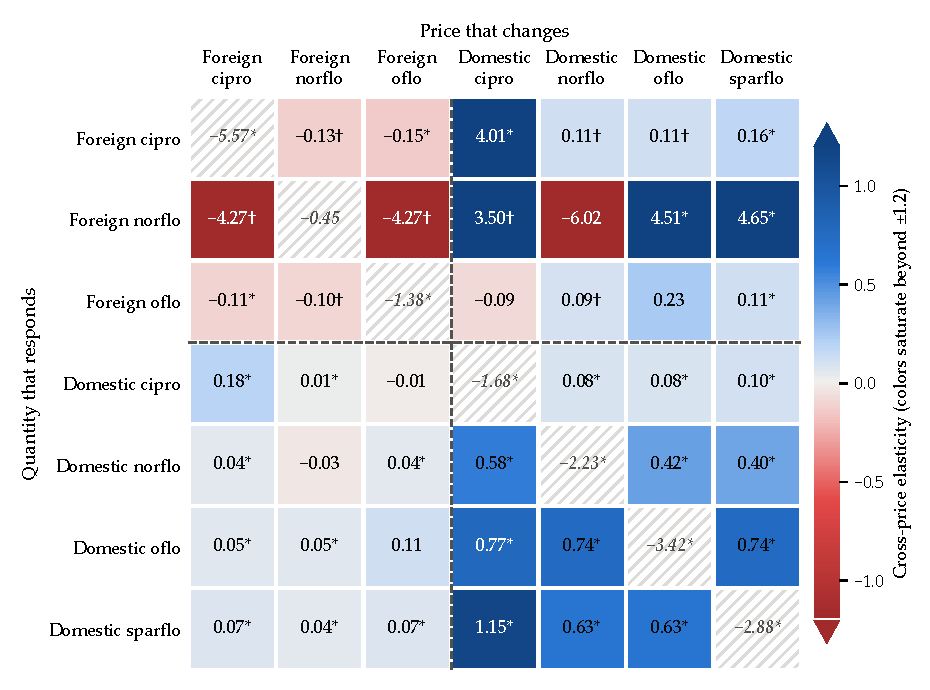
\includegraphics[width=\textwidth]{figures/ch05/cgj_table6a_heatmap.pdf}
\caption[Cross-price elasticities among quinolone groups]{Unconditional price elasticities among the seven
quinolone groups in the Northern region. Rows respond to the price in the column. Colors encode cross elasticities
(blue positive, red negative) and saturate beyond $\pm 1.2$. The hatched diagonal shows own-price elasticities, which
are excluded from the color scale. Marks: $^{*}$ significant at 5 percent, $^{\dagger}$ at 10 percent. Source:
constructed from Chaudhuri, Goldberg and Jia (2006), Table 6A.}
\label{fig:05-cgj-heatmap}
\end{figure}

\casehead{Ease of access} Why would a patient who loses domestic norfloxacin switch to domestic ofloxacin rather
than to foreign norfloxacin? The pattern is not built in by the specification, since the pair-type coefficients are
free in sign and size. CGJ propose an explanation based on distribution, which they call \emph{ease of access}
(pp.~27--28). Domestic firms as a group reach far more retail pharmacists than multinational subsidiaries. Large
Indian firms spread the fixed cost of medical representatives over larger portfolios, and there are simply many more
domestic firms and products. A local pharmacist is therefore more likely to stock two domestic molecules than the
domestic and foreign versions of one molecule. Patients or doctors who would rather switch molecules than search
another pharmacy then produce, in aggregate data, the substitution pattern of \cref{tab:05-cgj-table6a}. Together with
the domestic price premium of \cref{tab:05-cgj-table2}, the evidence shows no premium for multinational brands.

\casehead{The segment elasticity} The upper level (CGJ, Table~A3) gives a price elasticity of the quinolone segment
of $-1.11$, with standard error 0.24. Demand for the segment is elastic, but less so than demand for any single group
within it, except the tiny foreign norfloxacin group, whose insignificant own elasticity is $-0.45$. The number can be checked from the quinolone row of Table~A3, where $\gamma_{QQ} = -0.02$ and $\beta_Q =
0.04$. With the Northern quinolone share of antibiotic spending, $w_Q = \frac{31.25}{119.88} = 0.26$
(\cref{tab:05-cgj-table3}), the Stone-index formula gives
\begin{equation*}
\varepsilon_Q = -1 + \frac{\gamma_{QQ}}{w_Q} - \beta_Q = -1 - \frac{0.02}{0.26} - 0.04 = -1.12 .
\end{equation*}
This matches the reported value up to the rounding of $\gamma_{QQ}$ to two decimals.

\casehead{Robustness} CGJ report two alternative specifications (pp.~28--29). Adding group-specific seasonal effects
for summer, monsoon and winter leaves the elasticities nearly unchanged (Table~A4). Estimating the system by least
squares (Table~A5) gives smaller own elasticities in absolute value, as \eqref{eq:05-meas-bias} predicts.
\Cref{tab:05-cgj-robust} compares the own elasticities. The least-squares own elasticity of foreign ciprofloxacin is
$-2.76$, half the instrumented $-5.57$. Smaller elasticities would imply larger markups and larger welfare losses, so
instrumenting makes the welfare estimates more conservative. The least-squares cross elasticities among domestic
groups remain positive and significant. In the rows of domestic norfloxacin, ofloxacin and sparfloxacin they are
large (between 0.39 and 1.25), and they mostly exceed the same-molecule cross elasticities. CGJ call the close substitutability of domestic products ``one of the most robust findings of the
paper.''

\begin{table}[htbp]
\centering
\caption{Own-price elasticities under alternative specifications, Northern region}\label{tab:05-cgj-robust}
\small
\begin{tabular}{lccccc}
\toprule
 & Preferred (IV) & Least squares & \multicolumn{3}{c}{IV with seasonal effects} \\
\cmidrule(lr){4-6}
Product group & Table 6A & Table A5 & Summer & Monsoon & Winter \\
\midrule
Foreign cipro & $-5.57^{*}$ & $-2.76^{*}$ & $-6.06^{*}$ & $-5.80^{*}$ & $-5.66^{*}$ \\
Foreign norflo & $-0.45$ & 1.24 & 0.12 & $-0.35$ & $-0.20$ \\
Foreign oflo & $-1.38^{*}$ & $-0.99^{*}$ & $-1.58^{*}$ & $-1.51^{*}$ & $-1.55^{*}$ \\
Domestic cipro & $-1.68^{*}$ & $-1.56^{*}$ & $-1.72^{*}$ & $-1.72^{*}$ & $-1.73^{*}$ \\
Domestic norflo & $-2.23^{*}$ & $-2.18^{*}$ & $-2.04^{*}$ & $-2.10^{*}$ & $-2.22^{*}$ \\
Domestic oflo & $-3.42^{*}$ & $-3.16^{*}$ & $-3.67^{*}$ & $-3.20^{*}$ & $-3.08^{*}$ \\
Domestic sparflo & $-2.88^{*}$ & $-2.76^{*}$ & $-2.81^{*}$ & $-2.82^{*}$ & $-2.56^{*}$ \\
\bottomrule
\end{tabular}
\par\smallskip
\begin{minipage}{0.85\textwidth}\footnotesize
Notes: Compiled from CGJ, Tables~6A, A4(a) to A4(c), and A5. Standard errors omitted. $^{*}$ significant at 5 percent.
\end{minipage}
\end{table}

\begin{example}[Reproducing Tables 6A and 7 from Tables A2 and 3]\label{ex:05-cgj-elasticity-check}
The published coefficients, the published shares and the formulas of \cref{sec:05-cgj-demand} nearly reproduce the
published elasticities. We compute Northern revenue shares from the Northern sales in \cref{tab:05-cgj-table3}. Total
Northern quinolone sales of the seven groups are Rs.~1,563.56 million, so for example $w_7 = \frac{156.17}{1563.56} =
0.0999$ for domestic sparfloxacin.

\emph{Expenditure elasticities.} The elasticity with respect to quinolone spending is $\eta_i^Q = 1 +
\frac{\beta_i}{w_i}$. For domestic sparfloxacin,
\begin{equation*}
\eta_7^Q = 1 + \frac{-0.072}{0.0999} = 0.28,
\end{equation*}
exactly the value in Table~6A. \Cref{tab:05-cgj-checks} shows that the formula reproduces all seven entries of the
last column within 0.02.

\emph{Own-price elasticities.} The term $\beta_j\ln\frac{X_Q}{P_Q}$ in \eqref{eq:05-cgj-uncond-closed} depends on
$\alpha_0$ and on the units of prices, and CGJ do not report it. Setting it to zero gives our approximation. For
domestic sparfloxacin the conditional part is
\begin{equation*}
\varepsilon_{77}\big|_{X_Q} \approx -1 + \frac{\gamma_{77} - \beta_7w_7}{w_7}
= -1 + \frac{-0.186 + 0.072 \times 0.0999}{0.0999} = -2.79 .
\end{equation*}
The unconditional term adds $\eta_7^Q(1 + \varepsilon_Q)w_7 = 0.28 \times (-0.11) \times 0.0999 = -0.003$. The
approximation, $-2.79$, is close to the published $-2.88$. Across the 42 entries of Table~6A outside the foreign
norfloxacin row, the approximation has a root mean squared error of 0.036 and a largest error of about 0.15.
Choosing the omitted term to fit the table best lowers the root mean squared error only to 0.024. Most of the
remaining gap probably reflects the rounding of the published coefficients to three decimals.

\emph{Foreign norfloxacin.} Here the approximation fails. With $\gamma_{22} = 0.000$ and $w_2 = 0.0008$, it gives an
own elasticity of $-1.00$ against the published $-0.45$. Every coefficient in this row is divided by a share of 0.08
percent, which magnifies rounding and sampling error about 1,250 times. This is why the foreign norfloxacin row is so
imprecise in \cref{tab:05-cgj-table6a}.

\emph{Markups.} \Cref{sec:05-cgj-supply} shows that CGJ's upper bound on the Lerner index is $-\frac{1}{\varepsilon_{ii}}$.
The simple average of this ratio across the four regional own elasticities of Tables~6A and 6B reproduces every
markup in Table~7 to two decimals. For domestic oflo, for instance, the regional own elasticities $-3.42$, $-2.95$,
$-2.57$ and $-2.96$ give an average Lerner index of 0.34, the value in Table~7. The Northern ratio alone, 0.29, would
miss it.
\end{example}

\begin{table}[htbp]
\centering
\caption{Consistency checks: elasticities and markups recomputed from the published coefficients}\label{tab:05-cgj-checks}
\footnotesize
\setlength{\tabcolsep}{5pt}
\begin{tabular}{lccccccc}
\toprule
 & & \multicolumn{2}{c}{Expenditure elasticity} & \multicolumn{2}{c}{Own-price elasticity} & \multicolumn{2}{c}{Lerner index bound} \\
\cmidrule(lr){3-4}\cmidrule(lr){5-6}\cmidrule(lr){7-8}
Product group & \makecell{$w_i$\\ (North)} & $1 + \frac{\beta_i}{w_i}$ & Table 6A & Approx. & Table 6A &
\makecell{Mean of\\ $-\frac{1}{\varepsilon_{ii}}$} & Table 7 \\
\midrule
Foreign cipro & 0.0267 & 1.37 & 1.37 & $-5.50$ & $-5.57$ & 0.19 & 0.19 \\
Foreign norflo & 0.0008 & 2.22 & 2.20 & $-1.00$ & $-0.45$ & n.a. & n.a. \\
Foreign oflo & 0.0348 & 1.14 & 1.16 & $-1.38$ & $-1.38$ & 0.70 & 0.70 \\
Domestic cipro & 0.6154 & 1.17 & 1.17 & $-1.67$ & $-1.68$ & 0.59 & 0.59 \\
Domestic norflo & 0.1423 & 0.73 & 0.73 & $-2.22$ & $-2.23$ & 0.43 & 0.43 \\
Domestic oflo & 0.0800 & 0.90 & 0.89 & $-3.39$ & $-3.42$ & 0.34 & 0.34 \\
Domestic sparflo & 0.0999 & 0.28 & 0.28 & $-2.79$ & $-2.88$ & 0.37 & 0.37 \\
\bottomrule
\end{tabular}
\par\smallskip
\begin{minipage}{0.95\textwidth}\footnotesize
Notes: Our computations from CGJ's Tables~3, A2, 6A, 6B and 7. Shares are Northern sales shares among the seven
groups. ``Approx.''\ is \eqref{eq:05-cgj-uncond-closed} with $\ln\frac{X_Q}{P_Q}$ set to zero and $\varepsilon_Q =
-1.11$. The Lerner bound is the simple average across the four regions of minus the inverse own elasticity. For
foreign norfloxacin the own elasticity is below one in absolute value in every region, so no bound exists.
\end{minipage}
\end{table}

\subsection{Supply: bounds on costs and markups}\label{sec:05-cgj-supply}

The counterfactual needs marginal costs, which are not observed. The standard approach of \cref{ch:diffprod} infers
them from the first-order conditions of an assumed pricing game (\cref{sec:05-welfare-supply}). CGJ argue that price
regulation makes unconstrained period-by-period profit maximization untenable here, and the regulation is too complex
to model. They bound costs instead, using the argument of \cref{prop:05-cost-bounds}.

The bounds are those of \eqref{eq:05-cost-bounds} (CGJ, eqs.~3.12 and 3.13). Perfect competition within a group gives
the upper bound $c_i^U = p_i$ and a zero markup. Perfect collusion among the firms of group $i$, with price controls
ignored, gives the monopoly condition for the group as a whole. It yields the lower bound $c_i^L =
p_i\bigl(1 + \frac{1}{\varepsilon_{ii}}\bigr)$ and the upper bound $-\frac{1}{\varepsilon_{ii}}$ on the Lerner
index, where $\varepsilon_{ii}$ is the unconditional own-price elasticity. Collusion within the group overstates
market power, because it assumes away competition among the dozens of firms that sell each molecule (fn.~19).
Regulation pushes prices further below the monopoly level. Both forces keep the price at or below the group monopoly
price, as \cref{ass:05-conduct-order} requires, so $c_i^L$ is a lower bound. The bound requires $\varepsilon_{ii} < -1$. CGJ compute $c_i^L$ region by
region and report national averages.

\Cref{tab:05-cgj-table7} reproduces the bounds. The upper bound on profit is the upper-bound markup times revenue,
since $(p_i - c_i^L)q_i = \frac{p_i - c_i^L}{p_i}\,p_iq_i$. Annual sales of domestic ciprofloxacin, summed over the
regions of \cref{tab:05-cgj-table3}, are Rs.~2,931 million. Multiplying by a Lerner index of 0.586 gives about
Rs.~1,717 million, against Rs.~1,701.9 million in the table. The small gap reflects CGJ's population weights.

\begin{table}[htbp]
\centering
\caption{Bounds on marginal cost, markup and annual profit by product group}\label{tab:05-cgj-table7}
\small
\setlength{\tabcolsep}{4pt}
\begin{tabular}{lcccc}
\toprule
 & \multicolumn{3}{c}{Collusive bound} & Competitive bound \\
\cmidrule(lr){2-4}\cmidrule(lr){5-5}
 & \makecell{Lower bound for\\ marginal cost (Rs.)} & \makecell{Upper bound for\\ markup (\%)} &
 \makecell{Upper bound for\\ profit (Rs.\ million)} & \makecell{Upper bound for\\ marginal cost (Rs.)} \\
\midrule
Foreign cipro & $8.3^{*}$ & 19 & 26.9 & 10.3 \\
 & (1.23) & (0.12) & (16.55) & \\
Foreign norflo & n.a. & n.a. & n.a. & 5.3 \\
Foreign oflo & 32.3 & $70^{*}$ & $106.1^{*}$ & 108.5 \\
 & (23.16) & (0.21) & (31.85) & \\
Domestic cipro & $4.7^{*}$ & $59^{*}$ & $1{,}701.9^{*}$ & 11.2 \\
 & (1.14) & (0.10) & (298.58) & \\
Domestic norflo & $5.2^{*}$ & $43^{*}$ & $280.7^{*}$ & 9.0 \\
 & (0.20) & (0.02) & (15.32) & \\
Domestic oflo & $58.7^{*}$ & $34^{*}$ & $161.2^{*}$ & 90.1 \\
 & (2.18) & (0.02) & (12.80) & \\
Domestic sparflo & $49.5^{*}$ & $37^{*}$ & $198.5^{*}$ & 78.8 \\
 & (1.57) & (0.02) & (11.00) & \\
\bottomrule
\end{tabular}
\par\smallskip
\begin{minipage}{0.95\textwidth}\footnotesize
Notes: Reproduced from CGJ, Table~7. National averages of regional estimates. Standard errors in parentheses, with
markup standard errors expressed as fractions. $^{*}$ significant at 5 percent. The competitive bound sets marginal
cost equal to price, so the markup and profit are zero. CGJ's column heading labels the markup column ``(Rs.)'',
although its entries are percentages. No collusive bound exists for foreign norfloxacin, whose estimated own
elasticity is below one in absolute value.
\end{minipage}
\end{table}

The markup bounds are plausible (CGJ, p.~29). Domestic ciprofloxacin combines a high price, a large share and
relatively inelastic demand. It has one of the highest markup bounds (59 percent) and earns nearly 70 percent of the
sub-segment's profits. Indeed $\frac{1701.9}{2475.3} = 0.69$, where Rs.~2,475.3 million is the sum of the profit
column. Foreign ciprofloxacin faces the stiffest domestic competition and has the lowest bound (19 percent). The four
domestic profit bounds sum to Rs.~2,342 million. This number reappears below as the domestic profit loss when all
four domestic groups are withdrawn.

CGJ stress that these numbers are bounds. They do not measure actual costs. Regulation means the unconstrained
first-order condition need not hold, and aggregation across firms makes the collusive benchmark extreme. Most of their
counterfactuals use $c^L$, because it gives the largest possible profits. That is the worst case for Indian firms and
the best case for multinationals under patents.

\subsection{Counterfactual design}\label{sec:05-cgj-counterfactual}

\casehead{Scenarios} The benchmark is the most extreme policy. Foreign firms face no price controls, and
\emph{compulsory licensing} is unavailable. Under compulsory licensing a government authorizes other firms to produce
a patented drug in exchange for a royalty to the patent holder. CGJ consider five withdrawal scenarios, each removing
one or more domestic groups (p.~22).
\begin{enumerate}
\item Only domestic ciprofloxacin, a large group.
\item Only domestic ofloxacin, a small group.
\item Domestic ciprofloxacin, ofloxacin and norfloxacin.
\item Domestic ciprofloxacin, ofloxacin and sparfloxacin.
\item All four domestic groups.
\end{enumerate}
The remaining firms keep their product sets. The scenarios are illustrative. Most of the quinolone patents had expired
by the time of writing (norfloxacin's U.S.\ patent already in 1998), so none of the scenarios would materialize
(fn.~26). They show how the presence and extent of domestic competition affect the welfare calculation, which may
matter for therapeutic classes whose patents have not expired.

\casehead{The equilibrium system} Let $\mathcal{W}$ be the set of withdrawn groups. For each withdrawn group $i \in
\mathcal{W}$, the virtual price $p_{ir}^V$ sets its share to zero (CGJ, eq.~3.14):
\begin{equation}\label{eq:05-cgj-virtual}
\begin{split}
0 = {}& \alpha_{ir} + \gamma_{ii}\ln p_{ir}^V + \gamma_{i,10}\sum_{j\in D_i^{10}}\ln p'_{jr}
+ \gamma_{i,01}\sum_{j\in D_i^{01}}\ln p'_{jr} \\
&+ \gamma_{i,00}\sum_{j\in D_i^{00}}\ln p'_{jr} + \beta_i\ln\frac{X'_{Qr}}{P'_{Qr}}.
\end{split}
\end{equation}
Here $\alpha_{ir}$ now includes the common intercept, and $p'_{jr}$ is the new price of group $j$. A withdrawn group
$j$ enters the sums at its own virtual price. For each remaining group $k \notin \mathcal{W}$, the price solves the
group's monopoly first-order condition (CGJ, eq.~3.15):
\begin{equation}\label{eq:05-cgj-foc}
p'_{kr} = c_{kr}\left(1 + \frac{1}{\varepsilon_{kk}(p'_{r}, p^V_{r})}\right)^{-1}.
\end{equation}
The marginal cost $c_{kr}$ is set to $c^L_{kr}$ or $c^U_{kr}$. CGJ describe $\varepsilon_{kk}$ as the unconditional
own elasticity, a function of the new prices and the virtual prices (p.~23). The demand that a remaining group faces
also lets the virtual prices respond to its price. Its elasticity is therefore the rationed elasticity
\eqref{eq:05-rationed-elast-multi}. It combines the elasticities of \eqref{eq:05-cgj-uncond-closed} with the
unconditional share derivatives of the withdrawn groups, all at the virtual prices. CGJ do not say whether their $\varepsilon_{kk}$ includes this response. If it is the unrestricted
elasticity \eqref{eq:05-cgj-uncond-closed} evaluated at the virtual prices, \eqref{eq:05-cgj-foc} prices each group
against a demand curve that it does not face. The simulated prices are then an approximation. Quinolone spending $X'_{Qr}$ and the index $P'_{Qr}$ come from the upper level. The index
$P'_{Qr}$ is the translog of \eqref{eq:05-cgj-translog} at the new prices, and $X'_{Qr}$ follows from the upper-level
share at the new index, with the other sub-segments' price indices held fixed. The system is solved region by region.
National figures are population-weighted averages of the regional ones.

Equation~\eqref{eq:05-cgj-virtual} is the Marshallian zero-share condition at counterfactual spending, discussed in
\cref{sec:05-welfare-virtual}. Each withdrawn group's equation is quadratic in its log virtual price, because the
index $P'_{Qr}$ contains $\frac{1}{2}\gamma_{ii}(\ln p_{ir}^V)^2$ (\eqref{eq:05-virtual-quadratic}). With several
groups withdrawn the conditions must hold jointly. CGJ do not describe their solver. The block iteration of
\cref{sec:05-counterfactual}, which alternates between the virtual prices, the two budgeting levels and the pricing
conditions \eqref{eq:05-cgj-foc}, is one natural scheme. Foreign norfloxacin has no cost bound, so CGJ fix its counterfactual price at chosen values
and report that the results are robust to them (notes to Table~9).

\casehead{Welfare} Let $p^0$ be the observed price vector, $p'$ the counterfactual vector (virtual prices for the
withdrawn groups, new prices for the others), and $u^0$ the representative consumer's initial utility. Let $e(p, u)$
be the expenditure function of the upper-level AIDS, in which the lower level enters through the quinolone index
$P_Q$. CGJ measure the loss by
\begin{equation}\label{eq:05-cgj-cv}
CV^M = e(p', u^0) - e(p^0, u^0)
\end{equation}
(CGJ, eq.~3.16). It is positive for a loss. The virtual prices in $p'$ solve the Marshallian condition
\eqref{eq:05-cgj-virtual}, so they set Hicksian demand to zero at the counterfactual utility. As
\cref{sec:05-counterfactual} explains, \eqref{eq:05-cgj-cv} is therefore an approximation to the exact compensating
variation \eqref{eq:05-cv-exact}, which uses compensated virtual prices at $u^0$. The numbers below are CGJ's, computed
with \eqref{eq:05-cgj-cv}. CGJ split the loss into three parts with two intermediate price vectors. The
vector $p^1$ sets virtual prices for the withdrawn groups while holding $X_Q$ and all other prices fixed. The vector
$p^2$ recomputes the virtual prices letting $X_Q$ respond to the new quinolone index, again with all other prices
fixed. Then
\begin{equation}\label{eq:05-cgj-decomp}
CV^M = \underbrace{e(p^1, u^0) - e(p^0, u^0)}_{\text{pure loss of variety}}
+ \underbrace{e(p^2, u^0) - e(p^1, u^0)}_{\text{expenditure switching}}
+ \underbrace{e(p', u^0) - e(p^2, u^0)}_{\text{reduced competition}} .
\end{equation}
This is the general decomposition of \cref{sec:05-counterfactual} applied to CGJ's two levels. The first term is the
loss from the disappearance of products with everything else held fixed. It would be zero if consumers treated the
domestic and foreign versions of a molecule as identical, as earlier simulation studies assumed. The second term is
what CGJ call expenditure switching. It records how the Marshallian virtual prices shift when quinolone spending
responds to the higher index. The vector $p^2$ is the closest match to patents combined
with strict price regulation that holds the remaining prices at their pre-patent levels. The third term adds the price
increases of the remaining groups.

\casehead{Profits and national welfare} Profits are $\pi_k = (p'_k - c_k)q'_k$ at the counterfactual prices and
quantities. CGJ define Indian welfare as consumer welfare plus the profits of domestic firms. Foreign profits are
excluded, but CGJ compute them separately as a gauge of the incentive that Indian patents would give multinationals.
Losses are reported as positive numbers, so a negative domestic profit loss is a gain (fn.~38). With $c^L$, pre-patent
profits are at their largest, so the computed domestic profit loss is an upper bound.

\begin{remark}[The competitive cost bound in the simulation]\label{rem:05-cgj-cU}
The two cost bounds play different roles in \eqref{eq:05-cgj-foc}. With $c^L_{k} = p^0_k(1 + \frac{1}{\varepsilon_{kk}})$,
the observed prices satisfy \eqref{eq:05-cgj-foc} before any withdrawal, so simulated price changes are caused by the
withdrawal alone. With $c^U_k = p^0_k$ they do not. Before any withdrawal, \eqref{eq:05-cgj-foc} would already set
$p'_k = p^0_k\frac{\varepsilon_{kk}}{1 + \varepsilon_{kk}} > p^0_k$ whenever $\varepsilon_{kk} < -1$. The $c^U$
simulations therefore combine zero markups before the policy with group monopoly pricing after it. This reading may
explain why CGJ's Table~A6, which uses $c^U$, gives a much larger loss than Table~8 when only domestic ofloxacin is
withdrawn (Rs.~4.08 billion against 0.23). CGJ describe the $c^U$ losses as ``slightly higher'' and of the same order
of magnitude for the larger scenarios.
\end{remark}

\subsection{Counterfactual results}\label{sec:05-cgj-results}

\casehead{Consumer welfare} \Cref{tab:05-cgj-table8} reproduces CGJ's Table~8. All numbers in this subsection use
the cost lower bound $c^L$. The columns are cumulative. The first column holds $X_Q$ and the remaining prices fixed,
the second adds expenditure switching, and the third adds the price response of the remaining groups.

\begin{table}[htbp]
\centering
\caption{Consumer welfare losses from product withdrawal (Rs.\ billion per year)}\label{tab:05-cgj-table8}
\small
\begin{tabular}{lccc}
\toprule
 & & \multicolumn{2}{c}{Loss of variety and} \\
\cmidrule(lr){3-4}
\makecell[l]{Domestic groups\\ withdrawn} & \makecell{Pure loss\\ of variety} & \makecell{expenditure\\ switching} & \makecell{price adjustment and\\ expenditure switching} \\
\midrule
Only cipro & $4.98^{*}$ & $4.92^{*}$ & $7.32^{*}$ \\
 & (0.87) & (0.89) & (1.46) \\
Only oflo & 0.08 & 0.08 & $0.23^{*}$ \\
 & (0.08) & (0.08) & (0.10) \\
Cipro, oflo, norflo & $7.52^{*}$ & $7.40^{*}$ & $12.53^{*}$ \\
 & (1.77) & (1.80) & (4.15) \\
Cipro, oflo, sparflo & $6.14^{*}$ & $6.03^{*}$ & $10.58^{*}$ \\
 & (1.42) & (1.45) & (3.31) \\
All four & $11.76^{\dagger}$ & $11.35^{\dagger}$ & 17.81 \\
 & (6.43) & (6.34) & (12.70) \\
\bottomrule
\end{tabular}
\par\smallskip
\begin{minipage}{0.92\textwidth}\footnotesize
Notes: Reproduced from CGJ, Table~8 (identical to the published table). CGJ's welfare measure \eqref{eq:05-cgj-cv}, computed with the
cost lower bound. Standard errors in parentheses. $^{*}$ significant at 5 percent, $^{\dagger}$ at 10 percent. The
published table adds that the exchange rate is 45 rupees per U.S.\ dollar and that total sales of systemic
antibacterials in 2000 were Rs.~27 billion.
\end{minipage}
\end{table}

\Cref{fig:05-cgj-decomposition} splits each total into its three parts. In the all-four scenario the total loss is
Rs.~17.81 billion (CGJ, p.~31). The variety loss contributes Rs.~11.76 billion, or 66 percent of the total.
Expenditure switching reduces the loss by Rs.~0.41 billion ($-2$ percent). Price increases add a further Rs.~6.46
billion (36 percent). The shares are similar across scenarios. The variety loss accounts for 58 to 68 percent in every
scenario except the removal of ofloxacin alone, where the total is small.

\begin{figure}[htbp]
\centering
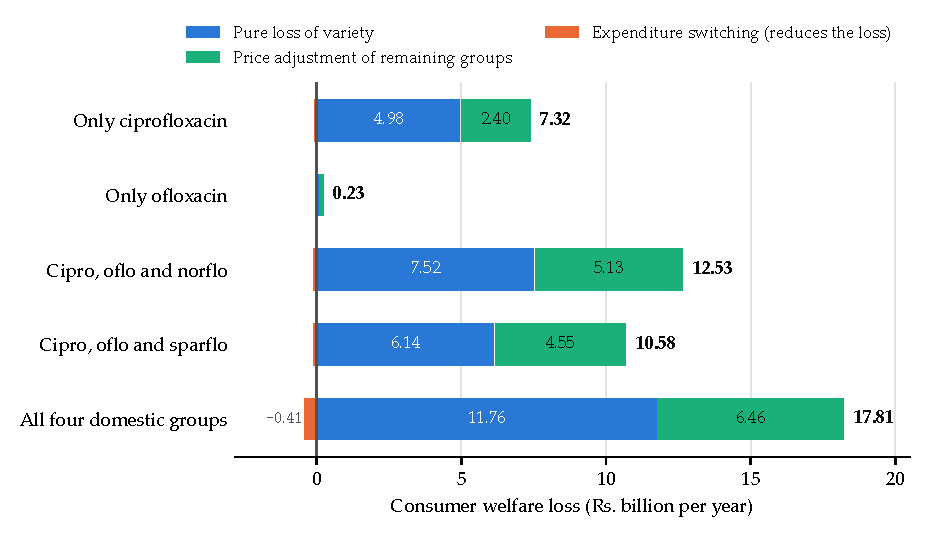
\includegraphics[width=\textwidth]{figures/ch05/cgj_welfare_decomposition.pdf}
\caption[Decomposition of the consumer welfare loss]{Decomposition of the consumer welfare loss in each withdrawal
scenario. Blue: pure loss of variety (Table 8, first column). Orange, left of zero: expenditure switching (second
column minus first). Green: price adjustment of the remaining groups (third column minus second). The bold number is
the total loss, equal to the blue and green segments minus the orange one. Standard errors are in
\cref{tab:05-cgj-table8}. Source: constructed from Chaudhuri, Goldberg and
Jia (2006), Table 8.}
\label{fig:05-cgj-decomposition}
\end{figure}

Three results matter for policy. First, expenditure switching is small in every scenario, although the segment
elasticity is $-1.11$. The reason is the factor $1 + \varepsilon_Q = -0.11$ derived above: a higher quinolone index
moves little spending out of the segment. Switching lowers the loss in four scenarios and leaves it unchanged when
only ofloxacin is withdrawn. CGJ read the term as consumers escaping to other sub-segments. Formally, the
upper-level expenditure function already lets consumers reallocate spending across sub-segments. The term arises
because the Marshallian zero-share condition \eqref{eq:05-cgj-virtual} moves the virtual prices when $X_Q$ falls
(\cref{sec:05-counterfactual}). The higher quinolone index lowers $X_Q$ slightly. That lowers the virtual price of a
withdrawn group with $\beta_i > 0$, such as domestic ciprofloxacin, and raises it for groups with $\beta_i < 0$. The
sign of the term is therefore not fixed by theory. For the claim of TRIPS proponents to hold, CGJ conclude, unpatented substitutes must exist
within narrowly defined therapeutic categories. Substitution across broad segments does little.

Second, the loss of variety is large. It arises only because consumers distinguish domestic from foreign versions of
the same molecule. CGJ interpret it as the ease-of-access effect. Price regulation cannot remove it, since regulation
acts on the third term. This suggests an independent role for compulsory licensing, which keeps domestic versions on
the market, either alongside price regulation or in its place.

Third, the losses are superadditive. Withdrawing all four domestic groups costs Rs.~17.81 billion. Withdrawing one
group at a time costs 7.32 (ciprofloxacin), 0.23 (ofloxacin), about 0.1 (norfloxacin) and close to zero (sparfloxacin),
for a sum of about Rs.~7.6 billion (fn.~37). The joint loss is more than twice the sum of the separate losses. The
three-group rows show the mechanism in our arithmetic. Adding sparfloxacin to the ciprofloxacin, ofloxacin and
norfloxacin withdrawal raises the loss from 12.53 to 17.81, by Rs.~5.28 billion. Adding norfloxacin to the other
triple raises it from 10.58 to 17.81, by Rs.~7.23 billion. Yet each costs at most Rs.~0.1 billion alone. When one
domestic group exits, consumers move to the other domestic groups, so the loss is small. When the last domestic group
exits, no close substitute remains. Studies that add up losses estimated market by market can therefore understate
the cost of patents substantially.

\casehead{Prices} \Cref{tab:05-cgj-table9} reports the counterfactual prices of the groups that remain. Shaded cells
in CGJ's table, dots here, mark withdrawn groups. Foreign norfloxacin's price is fixed by assumption.

\begin{table}[htbp]
\centering
\caption{Counterfactual prices of the remaining groups (\% of original prices)}\label{tab:05-cgj-table9}
\footnotesize
\setlength{\tabcolsep}{4pt}
\begin{tabular}{lccccccc}
\toprule
 & \multicolumn{3}{c}{Foreign groups} & \multicolumn{4}{c}{Domestic groups} \\
\cmidrule(lr){2-4}\cmidrule(lr){5-8}
Domestic groups withdrawn & Cipro & Norflo & Oflo & Cipro & Norflo & Oflo & Sparflo \\
\midrule
Only cipro & $189.4^{*}$ & 314.7 & $98.2^{*}$ & . & $148.6^{*}$ & $141.4^{*}$ & $164.1^{*}$ \\
 & (0.18) & & (0.21) & & (0.09) & (0.08) & (0.08) \\
Only oflo & $100.4^{*}$ & 150.0 & $102.9^{*}$ & $102.4^{*}$ & $108.3^{*}$ & . & $110.7^{*}$ \\
 & (0.01) & & (0.08) & (0.01) & (0.01) & & (0.01) \\
Cipro, oflo, norflo & $247.6^{*}$ & 627.8 & $154.4^{*}$ & . & . & . & $296.3^{*}$ \\
 & (0.42) & & (0.39) & & & & (0.70) \\
Cipro, oflo, sparflo & $255.2^{*}$ & 627.8 & $158.3^{*}$ & . & $250.1^{*}$ & . & . \\
 & (0.40) & & (0.37) & & (0.64) & & \\
All four & 396.4 & 627.8 & $318.4^{\dagger}$ & . & . & . & . \\
 & (3.34) & & (1.73) & & & & \\
\bottomrule
\end{tabular}
\par\smallskip
\begin{minipage}{0.95\textwidth}\footnotesize
Notes: Reproduced from CGJ, Table~9. Prices with expenditure switching and within-segment price adjustment, cost
lower bound. Dots mark withdrawn groups. Standard errors in parentheses. $^{*}$ significant at 5 percent,
$^{\dagger}$ at 10 percent. Foreign norfloxacin's price is fixed at the values shown, because its cost bound is not
available.
\end{minipage}
\end{table}

\begin{remark}[Reading Table 9]\label{rem:05-cgj-table9}
The heading of CGJ's Table~9 says the entries are percentages of original prices. Under that reading, foreign
ciprofloxacin's price would rise to 3.96 times its original level when all domestic groups exit, an increase of
about 296 percent. Two features of the table support the heading. The entries in the ofloxacin-only row are close to
100, which is what a small withdrawal should produce. The standard errors are of the order of 0.01 to 3.34, which
makes sense for ratios of new to old prices. CGJ's text reads the entries differently. It says that foreign prices
would rise ``between 100\% and 400\%'', the range of the foreign entries. It also says that the price of foreign
ciprofloxacin would be ``approximately 5 times higher than it is now'' in the all-four scenario. We report the
entries as printed and leave the ambiguity open. Under either reading, removing all domestic competition multiplies
the foreign prices several times.
\end{remark}

CGJ check plausibility against Pakistan, a country with similar demographics but a market structure close to what
patents would create in India, with multinational subsidiaries dominant. CGJ (p.~33), citing
\citet[p.~39, Table~2]{Lanjouw1998}, report that ciprofloxacin cost about seven times as much in Pakistan as in
India. CGJ's all-four prediction for foreign ciprofloxacin is of the same order of magnitude, though lower (p.~33).

The domestic groups that remain also raise their prices, by 41 to 64 percent when only ciprofloxacin is withdrawn
(reading the entries as percentages of original prices). These increases follow from the collusive conduct assumed
in \eqref{eq:05-cgj-foc}. A remaining domestic group is priced as if its 17 to 40 firms maximized joint profit, and
its demand becomes less elastic once a close domestic substitute disappears. The Le Chatelier principle of
\cref{sec:05-welfare-virtual} makes the second step precise. Let $i$ be the withdrawn group, whose virtual price
adjusts. The compensated own-price elasticity of a remaining group $j$ is then $\varepsilon^h_{jj} -
\varepsilon^h_{ji}\frac{p_jS_{ij}}{p_iS_{ii}}$ by \eqref{eq:05-le-chatelier-removed}, with all terms evaluated at the
virtual price. It is smaller in absolute value than the unrestricted compensated elasticity at that price. The
correction is largest for the closest substitutes, the other domestic quinolones. This channel is a
property of demand and holds under any conduct. Collusive conduct converts it into a large price increase. With
competitive pricing inside the group, the domestic price increases, and the third column of Table~8, would be smaller.

\casehead{Profits and total welfare} \Cref{tab:05-cgj-welfare-summary} combines CGJ's Tables~10, 11 and 12.

\begin{table}[htbp]
\centering
\caption{Domestic profit losses, total Indian welfare losses and foreign profit gains (Rs.\ billion per year)}\label{tab:05-cgj-welfare-summary}
\small
\begin{tabular}{lccc}
\toprule
 & & \multicolumn{2}{c}{Loss of variety and} \\
\cmidrule(lr){3-4}
\makecell[l]{Domestic groups\\ withdrawn} & \makecell{Pure loss\\ of variety} & \makecell{expenditure\\ switching} & \makecell{price adjustment and\\ expenditure switching} \\
\midrule
\multicolumn{4}{l}{\emph{Panel A. Foregone profits of domestic producers (Table 10)}} \\
Only cipro & $0.95^{*}$ (0.16) & $1.09^{*}$ (0.08) & 0.40 (0.31) \\
Only oflo & $-0.04^{*}$ (0.01) & $-0.03^{\dagger}$ (0.02) & $-0.14^{*}$ (0.04) \\
Cipro, oflo, norflo & $1.24^{*}$ (0.17) & $1.40^{*}$ (0.11) & 0.42 (0.60) \\
Cipro, oflo, sparflo & $1.11^{*}$ (0.17) & $1.26^{*}$ (0.11) & 0.48 (0.50) \\
All four & $2.34^{*}$ (0.19) & $2.34^{*}$ (0.19) & $2.34^{*}$ (0.19) \\
\addlinespace
\multicolumn{4}{l}{\emph{Panel B. Total welfare losses to India (Table 11)}} \\
Only cipro & $5.94^{*}$ (0.94) & $6.01^{*}$ (0.87) & $7.72^{*}$ (1.20) \\
Only oflo & 0.04 (0.08) & 0.05 (0.09) & 0.09 (0.10) \\
Cipro, oflo, norflo & $8.76^{*}$ (1.84) & $8.80^{*}$ (1.77) & $12.95^{*}$ (3.61) \\
Cipro, oflo, sparflo & $7.25^{*}$ (1.46) & $7.28^{*}$ (1.42) & $11.07^{*}$ (2.88) \\
All four & $14.10^{*}$ (6.57) & $13.70^{*}$ (6.48) & 20.16 (12.85) \\
\addlinespace
\multicolumn{4}{l}{\emph{Panel C. Profit gains of foreign producers (Table 12)}} \\
Only cipro & $0.17^{*}$ (0.03) & $0.14^{*}$ (0.06) & $0.35^{*}$ (0.17) \\
Only oflo & 0.02 (0.01) & 0.02 (0.01) & 0.01 (0.02) \\
Cipro, oflo, norflo & $0.36^{*}$ (0.05) & $0.28^{*}$ (0.11) & $0.71^{\dagger}$ (0.40) \\
Cipro, oflo, sparflo & $0.37^{*}$ (0.05) & $0.30^{*}$ (0.10) & $0.79^{*}$ (0.38) \\
All four & $1.17^{*}$ (0.31) & $0.88^{*}$ (0.41) & $2.43^{\dagger}$ (1.44) \\
\bottomrule
\end{tabular}
\par\smallskip
\begin{minipage}{0.95\textwidth}\footnotesize
Notes: Reproduced from CGJ, Tables~10, 11 and 12. Cost lower bound. Standard errors in parentheses. $^{*}$
significant at 5 percent, $^{\dagger}$ at 10 percent. Losses are positive numbers, so a negative entry in Panel A is a
gain for domestic firms as a group. Panel B equals Table~8 plus Panel A, up to rounding.
\end{minipage}
\end{table}

Domestic profits fall by Rs.~2.34 billion when all four groups exit, in every column. This is the whole pre-patent
profit of the domestic groups, the sum of the domestic profit bounds in \cref{tab:05-cgj-table7}. In the partial
scenarios, the remaining domestic firms gain from reduced competition, and these gains offset part of the losses.
When only ofloxacin is withdrawn, the domestic sector as a whole gains, because consumers switch to other domestic
molecules. This may explain why the Indian industry was divided over TRIPS. The association of leading Indian firms
and multinational subsidiaries supported stronger patents, while associations of smaller firms were more skeptical
(fn.~39).
In every scenario, consumer losses dwarf domestic profit losses.

Panel B is consumer loss plus domestic profit loss. The identity can be checked row by row. For the all-four scenario,
\begin{equation*}
13.70 \approx 11.35 + 2.34 \qquad\text{and}\qquad 20.16 \approx 17.81 + 2.34,
\end{equation*}
with the differences due to rounding. The columns of Panel A also show how expenditure switching and price responses
redistribute profits. When only ciprofloxacin is withdrawn, switching raises the domestic loss from 0.95 to 1.09,
because the remaining domestic groups sell less as quinolone spending falls. Price adjustment then cuts the loss to
0.40, because the remaining domestic groups raise their prices.

\casehead{The headline numbers} With the exchange rate of 45 rupees per dollar, CGJ's summary numbers follow from
Tables 8 to 12 (pp.~34--35).
\begin{itemize}
\item Without price regulation or compulsory licensing, the total welfare loss to India from withdrawing all four
domestic groups is Rs.~20.16 billion per year, about US\$450 million.
\item With regulation holding prices at pre-patent levels, the loss is Rs.~13.7 billion, about US\$305 million. This
is about 50 percent of the 2000 sales of all systemic antibacterials ($\frac{13.7}{27} = 0.51$). Foregone domestic
profits are about Rs.~2.3 billion (US\$50 million), roughly one-sixth of the total.
\item If the variety loss is transitional, or licensing could neutralize it, subtracting it leaves a lower bound of
Rs.~6.5 billion ($20.16 - 13.7$), about US\$144 million per year. The subtraction removes the variety loss (11.76),
the switching term ($-0.41$) and the domestic profit loss (2.34). The remainder equals the price-adjustment term of
\cref{tab:05-cgj-table8}, $17.81 - 11.35 = 6.46$. This is about 30 percent of the upper bound and about
24 percent of antibiotic sales in 2000.
\item Foreign profit gains are only Rs.~2.4 billion (US\$53 million) without regulation and Rs.~0.88 billion
(US\$19.6 million) with it.
\end{itemize}
CGJ put the foreign gains in perspective with the sales of Bayer's Cipro, about US\$1.6 billion in 2000. At a
markup of 40 percent, often quoted for the industry, that is about US\$640 million of annual profit from one product.
The gain from Indian patents on the whole quinolone segment would be a small fraction of this. Indian patents on
these drugs would hardly change multinationals' incentives to do research on the diseases of poor countries.

The welfare numbers are large relative to the market. Total quinolone sales in 2000 were near Rs.~5.7 billion, by
our computation from \cref{tab:05-cgj-table1}. The all-four consumer loss is about three times this amount
($\frac{17.81}{5.7} \approx 3.1$), and the variety loss alone about twice ($\frac{11.76}{5.7} \approx 2.1$).
Such numbers are possible because the compensating variation is an area under the Hicksian demand curve
up to the virtual price, far above observed prices. That area depends on the curvature of AIDS demand outside the
range of the data (\cref{sec:05-welfare-virtual}). The standard error of the all-four total loss, Rs.~12.70 billion,
reflects this uncertainty.

\casehead{The upper cost bound} Table~A6 repeats the consumer welfare calculation with $c^U$. The first two columns
are unchanged in point estimate, because they do not involve costs. The full loss in the all-four scenario is Rs.~19.46
billion, against 17.81 with $c^L$. CGJ explain that higher costs produce larger price increases. As
\cref{rem:05-cgj-cU} notes, the $c^U$ simulation also builds in price increases that would occur without any
withdrawal, which shows up clearly in the small scenarios.

\subsection{Interpretation, limitations and contribution}\label{sec:05-cgj-assessment}

CGJ draw three policy lessons. Product availability matters as much as affordability for consumer welfare, so patent
policy should be judged by both. Compulsory licensing has a role distinct from price regulation, because only the
former addresses the loss of variety. And the two policies are in tension. Patents without price controls strengthen
multinationals' incentives to build distribution networks or to license domestic firms, which would shrink the
variety loss over time. Price controls limit price increases but weaken these incentives, which could make the variety
loss permanent. No combination of policies is likely to neutralize all the welfare costs.

The study has several limitations, most of which CGJ acknowledge.
\begin{itemize}
\item \emph{Representative consumer.} The framework cannot say which households lose most. That would require micro
data on purchases, which do not exist for Indian pharmaceuticals (fn.~30). The aggregate compensating variation is
also a statement about a representative household, as discussed in \cref{sec:05-aggregation}.
\item \emph{Uniform pricing.} The model rules out price discrimination, which could change both welfare losses and
profit gains (fn.~31).
\item \emph{Static analysis.} The model has no research response, no new launches and no investment in distribution.
The product sets of the remaining firms are held fixed. If foreign firms expand distribution, alone or through joint
ventures with Indian firms, the ease-of-access loss would be transitional. CGJ report media accounts of such
initiatives.
\item \emph{Aggregation and conduct.} Groups aggregate dozens of firms, and the cost bound $c^L$ treats each group as a
cartel. This inflates pre-patent markups and the price responses of the remaining domestic groups.
\item \emph{Functional form and extrapolation.} Virtual prices lie far outside the observed price range. The welfare
loss, several times the segment's sales, depends on AIDS curvature where no data exist. Logit or CES demand would
give different answers, as \cref{prop:05-variety} shows.
\item \emph{Identification.} The SKU-count instruments fail if SKU entry responds to demand shocks or raises demand
directly. Domestic ciprofloxacin, the most important group, has the weakest first stage and little price variation
over time.
\item \emph{Restrictions.} The pair-type restriction forces one coefficient on all domestic pairs, and homogeneity then
ties the own-price coefficients to the cross coefficients (\cref{prop:05-cgj-collapse}). The ease-of-access pattern is
estimated, but its uniformity across domestic pairs is imposed.
\item \emph{Small foreign groups.} Foreign norfloxacin's estimates are unreliable, and the negative cross elasticities
among foreign groups are unexplained.
\item \emph{Revealed preference.} Doctors choose most prescriptions, and they or their patients may err or follow
promotion. If choices do not reflect informed preferences, welfare computed from them may mislead. Antibiotic use also
has external effects, such as bacterial resistance, that private demand ignores.
\end{itemize}
Several open questions follow. Did TRIPS spur research, including by Indian firms? Is Pakistan a credible benchmark
for post-patent prices in India? Which consumers rely most on domestic firms? Would ease of access persist once
multinationals expand distribution or license their molecules?

The paper made three contributions. It gave the first estimates of the welfare effects of TRIPS that rest on estimated
demand and cost parameters, where earlier studies had assumed them. It allowed consumers to distinguish domestic from
foreign versions of the same molecule, which revealed a variety channel that price-based analyses miss. And it
estimated cross-price effects flexibly, which showed that losses compound when several domestic groups disappear.
Methodologically, it shows how a multi-level AIDS, simple instruments, cost bounds and virtual prices combine into a
transparent counterfactual.

\begin{table}[htbp]
\centering
\caption{Identification and counterfactual map of Chaudhuri, Goldberg and Jia (2006)}
\label{tab:05-cgj-map}
\footnotesize
\renewcommand{\arraystretch}{1.1}
\begin{tabularx}{\textwidth}{@{}>{\raggedright\arraybackslash}p{2.6cm}>{\raggedright\arraybackslash}X@{}}
\toprule
Observed data & Monthly retail sales and prices of quinolone antibiotics in four Indian regions, 1999 and
  2000, from the ORG-MARG audit. Stock-keeping units are aggregated into seven groups by molecule and
  domestic or foreign status. Spending on all systemic antibacterials. \\
\addlinespace
Latent objects & Exact group price indexes and the error of their revenue-weighted proxies, demand shocks,
  marginal costs, and the virtual prices of withdrawn groups. \\
\addlinespace
Estimated parameters & Lower-level AIDS coefficients under pair-type restrictions, upper-level AIDS
  coefficients for eight antibacterial sub-segments, and group-region effects. \\
\addlinespace
Identifying variation & Numbers of SKUs and prices of the five largest SKUs of each group, by region and
  month (\cref{ass:05-cgj-iv}). Regulated SKU prices change rarely, so group prices move mostly with the
  SKU mix. \\
\addlinespace
Maintained assumptions & Two-stage budgeting with a representative consumer and uniform pricing. SKU entry
  is unrelated to demand shocks. Cost bounds replace a model of conduct under price regulation
  (\cref{prop:05-cost-bounds}). \\
\addlinespace
Counterfactual and what it holds fixed & Withdrawal of one or more domestic groups, with virtual prices for
  the withdrawn groups and group monopoly pricing of the others at the cost bounds. The product sets of the
  remaining firms and the prices of other sub-segments are held fixed. \\
\addlinespace
Conclusion & Withdrawing all four domestic groups costs India Rs.~20.16 billion a year, about US\$450
  million, without price regulation and Rs.~13.7 billion with it. Most of the consumer loss is lost
  variety, valued by AIDS curvature far beyond observed prices. \\
\addlinespace
One limitation & The losses, several times the segment's sales, depend on the functional form of demand
  where no data exist. \\
\addlinespace
Source and our additions & The tables are CGJ's. \Cref{prop:05-cgj-collapse}, \cref{ex:05-cgj-elasticity-check},
  \cref{rem:05-cgj-cU} and the recomputed elasticities and markups of \cref{tab:05-cgj-checks} are ours. \\
\addlinespace
Tools in the appendices & \Cref{sec:A-iv,sec:A-delta-boot,sec:B-duality}. \\
\bottomrule
\end{tabularx}
\end{table}

\section{Retrospective evidence: what happened after patents arrived}\label{sec:05-dgg}

CGJ's analysis is prospective in the sense of \cref{sec:05-questions}. It predicts the effects of a policy before the
policy exists. India introduced product patents for pharmaceuticals in 2005, and a retrospective analysis then
became possible. Such an analysis measures what happened after the policy, using variation in its timing or reach.
\citet{DugganGarthwaiteGoyal2016} (DGG henceforth) provide it. This section reports their setting, design and main
results and asks why the two answers differ.\footnote{We cite the published article in the \emph{American Economic
Review} 106(1), 2016. Page, table, equation and footnote numbers refer to it.}

\subsection{Setting and data}\label{sec:05-dgg-setting}

TRIPS required product patents in all fields of technology, with a minimum term of 20 years. India had no product
patents when TRIPS came into force in 1995, so it received a transition period of ten years (DGG, p.~105). From 1995 a
``mailbox'' collected patent applications, and the government published neither their number nor their content. The
2005 reform kept several flexibilities. A grandfather clause lets a generic firm that invested in a molecule before
2005 continue to produce it after paying a ``reasonable royalty'' to the patent holder. DGG call this a de facto
compulsory license for existing generic producers (p.~106). Section 3(d) of the amended Act limits patents on chemical
entities known before 1995 to inventions with significantly greater therapeutic efficacy (p.~107).

Compulsory licensing and price controls also remained available, but India used them sparingly. Its first compulsory
license came in March 2012. Natco was allowed to sell a generic version of Bayer's cancer drug Nexavar for a royalty of
6 percent, at about \$176 a month against Bayer's \$5,600 (p.~106). Price controls covered only 74 drugs until 2013,
when they were extended to nearly 350 (p.~106). DGG add that the mere threat of these tools may have restrained prices
(p.~101).

The timing of grants was hard to predict. The first pharmaceutical product patent, for Roche's hepatitis C drug
Pegasys, came only in 2006 (pp.~107 and 110). That was more than a year after the mailbox applications were opened for review
on 1 January 2005 (p.~107). Section 3(d) also left the patent office wide discretion (p.~107). In April 2013 the Supreme Court
upheld the denial of a patent for Novartis's cancer drug Glivec, which the office had judged an incremental change to
an older compound (fn.~5). DGG argue that this uncertainty makes the date of a grant a plausibly exogenous shock to
each molecule's market (pp.~107--108).

The sales data are quarterly retail sales from the MIDAS database of IMS Health. They come from an audit of about
5,100 stockists that covers 80 to 85 percent of the Indian market (p.~108). DGG use all single-molecule products,
which account for over half of sales (p.~109). The estimation sample runs from the second quarter of 2004 to the end
of 2011. It keeps molecules with positive sales in the first quarter of 2005 (p.~108 and fn.~8). It contains more
than 6,000 products and about 1,000 molecules (p.~101). A patent search firm matched granted Indian patents to
molecules by keyword searches. About one-third of the molecules are covered by at least one product patent by the end
of 2011. The outcomes are aggregated to the molecule-quarter level. They are the log of the average price per
standard unit, the log of quantity, the number of selling firms and the Herfindahl index of sales.

\subsection{Design}\label{sec:05-dgg-design}

The identifying variation is the timing of patent grants. Different molecules received Indian patents in different
quarters after the 2005 amendment. If the timing of a grant is unrelated to other changes in a molecule's market,
molecules that have not yet received a patent serve as controls for those that have. Let $m$ index molecules and $t$
quarters. The baseline regression is DGG's eq.~(1),
\begin{equation}\label{eq:05-dgg-dd}
Y_{mt} = \mu_m + \tau_t + \vartheta\, t\cdot\indic\{\text{ever patented}\}_m
  + \phi\,\indic\{\text{has patent}\}_{mt} + u_{mt}.
\end{equation}
Here $\mu_m$ are molecule fixed effects and $\tau_t$ year-by-quarter fixed effects. The third term gives molecules that
receive a single-molecule patent during the sample their own linear trend. The indicator
$\indic\{\text{has patent}\}_{mt}$ equals one in the quarters in which molecule $m$ is covered by at least one
single-molecule patent. DGG write $\alpha_m$, $\delta_t$, $\lambda$ and $\beta$ for the coefficients, which we rename to
avoid clashes with the AIDS parameters. The coefficient $\phi$ is a difference in differences. It compares the change
in a molecule's outcome when its patent arrives with the change over the same quarters for molecules without a patent.
Standard errors are clustered by molecule.

The event-study version is DGG's eq.~(2). Let $g_m$ be the quarter in which molecule $m$ receives its first patent and
$\bar p_{mt}$ the average price of its products. Then
\begin{equation}\label{eq:05-dgg}
\ln\bar p_{mt} = \mu_m + \tau_t + \sum_{k\neq 0}\phi_k\,\indic\{t - g_m = k\} + u_{mt}.
\end{equation}
The event-time indicators run from $k = -8$ to $k = 8$. DGG write the limits of the sum as $-8+$ and $8+$, so the
end points bin all earlier and all later quarters. The grant quarter $k = 0$ is the omitted category, and the
molecule-specific trend is dropped. Each $\phi_k$ measures the average log price $k$ quarters from the grant, relative
to the grant quarter and net of molecule and quarter effects.

Identification rests on two assumptions. Absent patents, log prices of molecules with early and late grants would
have moved in parallel. And prices do not respond before the grant. The leads $\phi_k$ for $k < 0$ test both, since
they should be near zero. DGG also probe anticipation directly. For molecules whose first application sat in the
mailbox, firms knew least about the timing of the decision. The estimate of $\phi$ for this sample is 0.025 (0.012),
against 0.027 (0.013) for the full sample (fn.~22). With staggered timing and effects that vary across molecules or
over event time, two-way fixed-effects regressions like \eqref{eq:05-dgg-dd} can weight effects in unintended ways.
Estimators robust to this problem are discussed in \cref{app:econometrics}.

\subsection{Results}\label{sec:05-dgg-results}

\Cref{fig:05-dgg} reproduces DGG's Figure~1. Before the grant, the point estimates lie close to zero, and the
confidence bands include zero in every quarter. Prices begin to rise in the first quarters after the grant. From the
third quarter on, the estimates are about 0.036 to 0.041, and the lower confidence bound lies just above zero in
quarters 3 to 7. The bound for the binned quarter 8+ includes zero.

\begin{figure}[htbp]
\centering
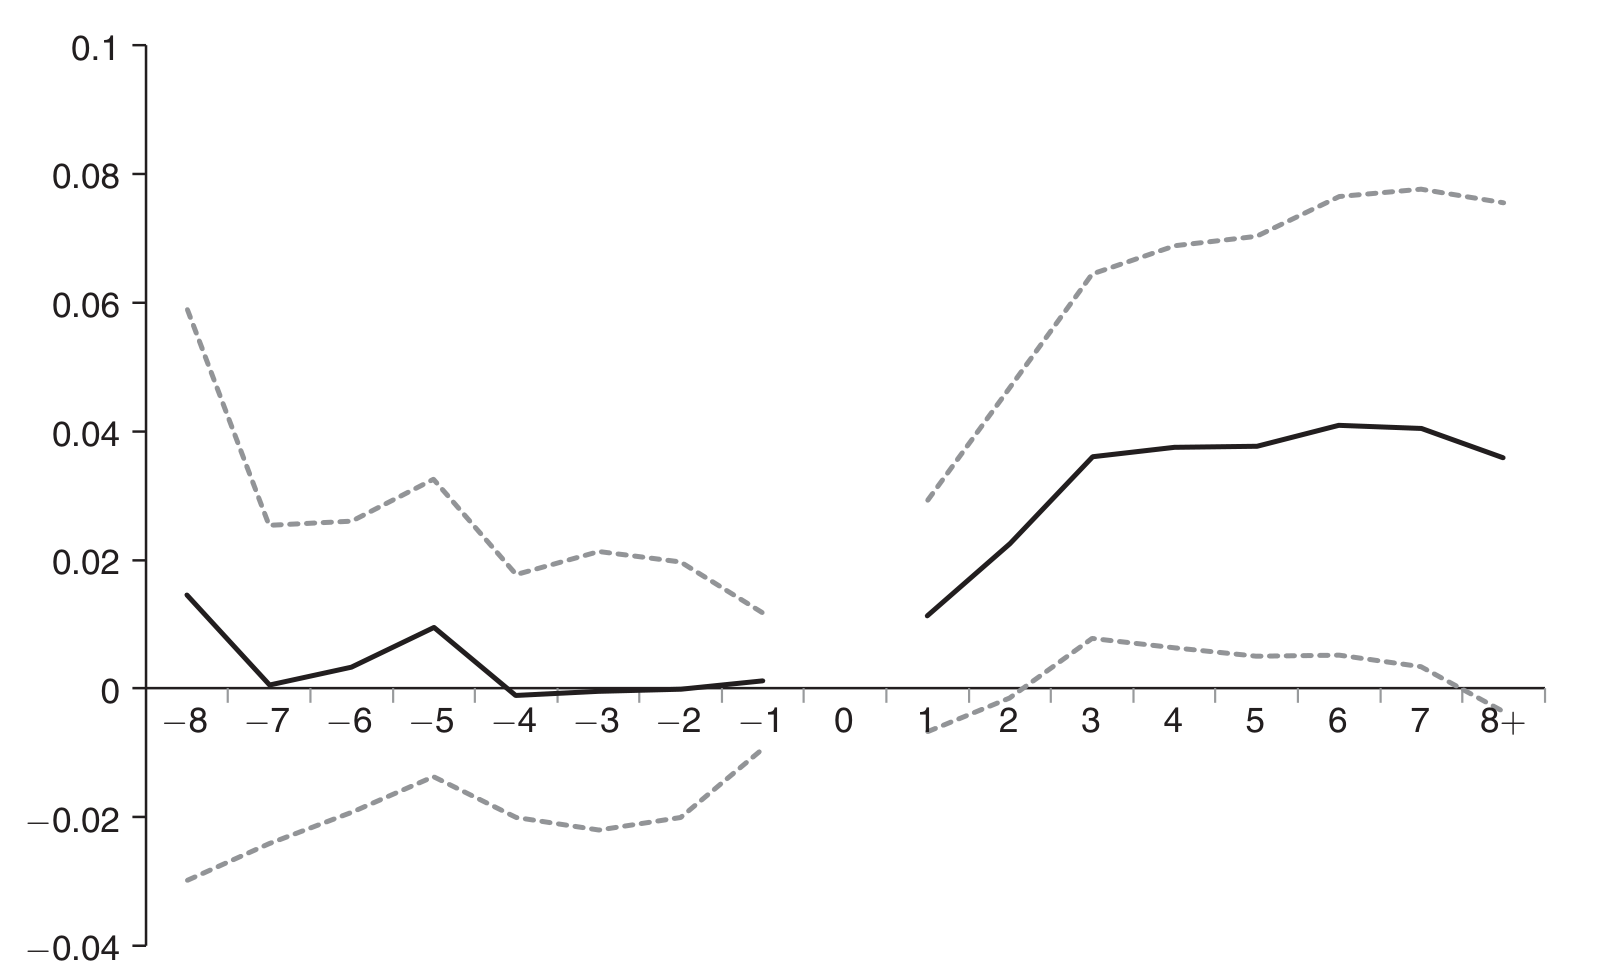
\includegraphics[width=0.85\textwidth]{figures/ch05/dgg_fig1.png}
\caption[Event-study estimates of patent effects on prices in India]{Event-study estimates for the log of the average
price before and after a patent is granted, from \eqref{eq:05-dgg}. The horizontal axis shows quarters relative to
the grant, from $-8$ to $8+$, and the end points bin all earlier and all later quarters. The solid line shows point
estimates and the dashed lines show 95 percent confidence intervals, with standard errors clustered by molecule. The
grant quarter is the omitted category. Source: Duggan, Garthwaite and Goyal (2016), Figure 1.}
\label{fig:05-dgg}
\end{figure}

\Cref{tab:05-dgg} collects the difference-in-differences estimates. In the full sample a patent raises the average
price of a molecule by 2.7 percent, and the 95 percent confidence interval rules out increases above 5.3 percent
(p.~117). Among molecules that are eventually patented, where only the timing of grants varies, the estimate falls to
0.016 and is insignificant. Patents matter more for newer molecules. Among patented molecules, those first sold in
India after 1995 see prices rise 4.9 percent more than older ones. The estimate for older molecules is $-0.014$
(0.012). In the sample of molecules approved in the United States between 1996 and 2004, patented molecules see their
prices rise by about 6 percent relative to molecules with pending applications (Table~5).

\begin{table}[htbp]
\centering
\caption{Effects of a patent grant on molecule outcomes in India}\label{tab:05-dgg}
\small
\begin{tabular}{l>{\raggedright\arraybackslash}p{5.2cm}ccc}
\toprule
Outcome & Sample and coefficient & Estimate & Molecules & Obs. \\
\midrule
Log price & All molecules, has patent & 0.027 & 1,012 & 29,845 \\
 & & (0.013) & & \\
Log price & Patented molecules, has patent & 0.016 & 335 & 10,264 \\
 & & (0.013) & & \\
Log price & Patented molecules, has patent $\times$ post-1995 & 0.049 & 335 & 10,264 \\
 & & (0.022) & & \\
Log price & U.S.-approved 1996--2004, has patent & 0.061 & 46 & 1,236 \\
 & & (0.029) & & \\
Log price & Post-1995 molecules, has patent $\times$ only firm in 2005 & 0.169 & 651 & 18,908 \\
 & & (0.099) & & \\
Log quantity & All molecules, has patent & $-0.054$ & 1,012 & 29,853 \\
 & & (0.036) & & \\
Number of firms & All molecules, has patent & $-0.390$ & 1,012 & 29,853 \\
 & & (0.268) & & \\
Herfindahl index & All molecules, has patent & 0.014 & 1,012 & 29,853 \\
 & & (0.007) & & \\
\bottomrule
\end{tabular}
\par\smallskip
\begin{minipage}{0.94\textwidth}\footnotesize
Notes: OLS estimates of \eqref{eq:05-dgg-dd} with molecule and year-by-quarter fixed effects. Standard errors clustered
by molecule in parentheses. Rows 1, 2 and 6: DGG Table~4, columns 1, 2 and 5. Rows 7 and 8: Table~7, columns 1 and
5. Row 3:
Table~4, column 4, the triple difference of DGG's eq.~(3). Row 4: Table~5, column 1, molecules granted a patent or
with a pending application. Row 5: Table~6, column 1, the interaction term only. The main effect of a patent in that
regression is 0.026 (0.022). The Herfindahl index is measured on a scale from 0 to 1.
\end{minipage}
\end{table}

The mechanism points to the grandfather clause. Among molecules first sold after 1995, the main effect of a patent,
which applies to molecules with several producers in 2005, is 0.026 (0.022), small and insignificant (Table~6). The
interaction coefficient of 0.169 (0.099) is the additional log price effect for a molecule that had only one producer
in 2005. The total effect for such a molecule is the sum, 0.195 log points or about 21.5 percent. DGG do not report a
standard error for this sum, and they describe the interaction alone as a nearly 20 percent increase (p.~122). Where
generic producers already existed,
the royalty rule let them keep selling, and the patent holder's pricing power stayed limited (p.~122). The number of
firms barely changes, and the Herfindahl index of the molecule's sales rises by 0.014 (Table~7). Sales shift toward
the patent holder without exit by the incumbents. The price effects are also concentrated in molecules with small
sales. Molecules with one producer sold about \$0.10 million a quarter, against \$1.28 million for the others
(p.~125). Weighting the post-1995 regression by sales turns an estimate of 0.054 (0.019) into $-0.003$ (0.016)
(fn.~28). DGG summarize the price effect of a patent as an average increase of 3 to 6 percent, with little effect on
quantities or on the number of firms (p.~99). They add that the single-producer molecules resemble future innovations,
which will face no generic rival when their patents are granted (pp.~124--125).

\subsection{Why the forecast and the evidence differ}\label{sec:05-forecast-gap}

CGJ's text describes foreign price increases of between 100 and 400 percent (see \cref{rem:05-cgj-table9} for the
reading of their Table~9). DGG measured 3 to 6 percent. Is the model wrong, or did the policy differ from the scenario
that CGJ simulated? DGG themselves doubt that demand is the explanation. CGJ's estimates imply that an unregulated
monopolist would set a price at least twice the pre-patent price (DGG, p.~122). Most of the gap comes from the
scenario.
\begin{itemize}
\item \emph{Which molecules.} Under the transition rules, product patents could be granted only for inventions whose
applications were filed from 1995 onward. Older molecules, including all four quinolones, stayed open to generic
competition. CGJ themselves note that most quinolone patents had expired and that none of their scenarios would
materialize (fn.~26).
\item \emph{Grandfathering.} Indian firms already producing drugs whose patent applications were filed between 1995
and 2005 may continue to produce them on payment of a royalty (CGJ, fn.~6, and DGG, p.~106). A patent grant therefore
need not remove domestic versions from the market, which is exactly the event CGJ simulate. DGG's estimates for
molecules with one producer in 2005 show what happens when no domestic version remains.
\item \emph{Scope of patents.} Section 3(d) limits patents on new forms of known substances. It restricts the practice
of extending protection through minor changes to a molecule, as the Glivec decision showed.
\item \emph{Remaining policy tools.} Compulsory licensing and price controls stayed available, even if they were rarely
used. In CGJ's framework, compulsory licensing targets the first term of \eqref{eq:05-cgj-decomp} and price controls
target the third.
\item \emph{Timing.} The reform was announced a decade in advance, and grants arrived one molecule at a time. CGJ's
scenario is a sudden withdrawal of all domestic versions of a molecule, with no regulation, which they present as the
most extreme case.
\end{itemize}

The two studies also measure different objects. CGJ's percentages are the price changes of a remaining foreign group
after every domestic competitor of the molecule disappears. DGG's estimate averages over all products in molecules that
received patents under the rules India adopted, including molecules where domestic versions remained. The
mechanisms CGJ identify, the loss of variety through ease of access and the compounding of losses across close
domestic substitutes, are not refuted by DGG. They were not tested, because the simulated event did not occur.

The episode teaches a general lesson. A counterfactual is only as relevant as the policy scenario it simulates.
Prospective and retrospective analyses complement each other. The prospective model gives welfare numbers and
mechanisms for policies not yet tried, while the retrospective study measures the effects of the policy that was
chosen. A credible prospective study should therefore simulate the policy most likely to be adopted, alongside the
extreme case.

\section{Assessment: what product-space demand can and cannot do}\label{sec:05-assessment}

The AIDS is a flexible demand system in product space with an explicit link to preferences. It is a first-order
approximation to any demand system (\cref{prop:05-flexible}), and the restrictions of utility maximization are linear
in its parameters (\cref{prop:05-restrictions}). It aggregates across households of different incomes through a
representative budget level (\cref{sec:05-aggregation}). Its expenditure function gives the compensating variation in
closed form, and its finite virtual prices let it value the withdrawal of a product (\cref{sec:05-welfare}).
Combined with first-order conditions or cost bounds, it supports counterfactual equilibria, as CGJ show. At the point
of approximation, only theory restricts its substitution patterns. This flexibility is its main advantage over logit
and CES demand.

The costs are equally clear. The number of price parameters grows with the square of the number of products, about
$\frac{J^2}{2}$, so applications need a few product groups and a multi-stage budgeting tree. Two-stage budgeting
requires separability assumptions that restrict substitution across groups (\cref{sec:05-separability}), and the
grouping must be chosen before estimation. Each price needs an instrument, and product-space parameters are product
specific, so the characteristics-based instruments of discrete-choice models are unavailable. CGJ go further and
impose pair-type restrictions, which tie own-price effects to cross effects. Welfare numbers for disappearing products
rest on the curvature of demand far outside the data. Merger simulations show that this curvature matters: AIDS tends
to predict larger price effects than logit or linear demand \citep{CrookeEtAl1999}.

Counterfactual results from such a model are informative, but they depend on three choices. The functional form fixes
the shape of demand beyond the data. The instruments determine whether the elasticities are credible. And the
simulated scenario must match the policy that will be adopted. The CGJ and DGG comparison shows how the third choice
can dominate the other two.

The alternative is to model demand in the space of characteristics. Products become bundles of a few attributes, so
the number of parameters no longer grows with the square of the number of products. New and withdrawn products are
handled naturally, and characteristics of rival products supply instruments. The price is a different set of
assumptions: an idiosyncratic taste shock for every product and functional forms for the distribution of tastes.
\Cref{ch:discrete} develops the discrete-choice foundations, \cref{ch:logit} the logit and nested logit models with the
inversion of \citet{Berry1994}, and \cref{ch:blp} random-coefficient models such as \citet{Nevo2001}. The valuation
of new goods, the mirror image of CGJ's withdrawals, returns in \cref{ch:newgoods} with the multi-level demand system
of \citet{Hausman1997}. Merger simulation with estimated demand systems is the subject of \cref{ch:mergers}.


\section{Bibliographic notes}\label{sec:05-bibnotes}

The AIDS belongs to a line of work on demand systems that are consistent with utility maximization and flexible
enough to test it. The linear expenditure system of \citet{Stone1954} was the first such system estimated from an
explicit utility function. The Rotterdam model of \citet{Theil1965} and \citet{Barten1969} and the translog model of
\citet{ChristensenJorgensonLau1975} added flexibility, a property that \citet{Diewert1974} defined formally.
\citet{DeatonMuellbauer1980a} combined the virtues of these models. Their book \citep{DeatonMuellbauer1980b}
remains the standard reference. Its \S 3.4 (pp.~75--78) derives the AIDS from Working-Leser Engel curves and
tests homogeneity on the British data. Chapter~5 (pp.~119--147) treats separability and two-stage budgeting, and
chapter~6 (pp.~148--166) treats market demand and aggregation. Its \S 4.3 (pp.~109--114) covers rationing and shadow
prices, and \S 7.1 (pp.~170--179) cost-of-living indices. \citet{Deaton1978} discusses specification and testing in
applied demand analysis.

The theory of aggregation starts with the exact aggregation results of \citet{Gorman1953,Gorman1961}.
\citet{Muellbauer1975,Muellbauer1976} introduced the PIGL and PIGLOG classes and the representative budget level
that underlie the almost exact aggregation of the AIDS. The Engel curves of \citet{Working1943} and \citet{Leser1963}
motivated the logarithmic form. \citet{Gorman1981} bounded the rank of exactly aggregable demand systems,
\citet{Lewbel1991} defined the rank and showed how to estimate it, and \citet{BanksBlundellLewbel1997} proposed the
quadratic AIDS. \citet{HurwiczUzawa1971} give conditions under which a demand system is generated by preferences.
\citet{Gorman1959} characterized two-stage budgeting, and \citet{GoldmanUzawa1964} and \citet{Gorman1971} derived
its implications for substitution. \citet{BartenTurnovsky1966} showed that weak separability alone supports a first
stage with two price indices per group, and \citet{Gorman1970} introduced implicit separability.
\citet{BlackorbyPrimontRussell1978} give a comprehensive treatment of separability. On index numbers,
\citet{Diewert1976} established when the Tornqvist index is exact.

Several papers address the econometrics of the AIDS. \citet{Barten1969} showed that maximum likelihood estimates do
not depend on which share equation is dropped. \citet{Moschini1995} analyzed the units problem of the Stone index,
and \citet{GreenAlston1990} the computation of elasticities in the linear approximate model. \citet{Lau1978} and
\citet{Moschini1999} show how to impose curvature through a Cholesky factorization. On the welfare side, the virtual
prices of \citet{Hicks1940} and \citet{Rothbarth1941} value products that are absent from the market.
\citet{Willig1976} bounds the gap between Marshallian surplus and the exact measures, and \citet{HausmanNewey1995}
estimate exact consumer surplus nonparametrically.

Industrial organization adopted the multi-level AIDS for antitrust and policy analysis.
\citet{HausmanLeonardZona1994} estimated it for beer, identified it with prices in other cities, and used it to
simulate mergers. \citet{Hausman1997} applied the same framework to value a new cereal brand, and the comment of
\citet{Bresnahan1997} questioned both the instruments and the competitive assumptions. \citet{EllisonEtAl1997}
estimated a multi-stage AIDS for cephalosporin antibiotics, and \citet{HausmanLeonard2002} studied the competitive
effects of a new product introduction. The instruments draw on the panel-data logic of \citet{HausmanTaylor1981},
and their validity can be probed with the specification test of \citet{Hausman1978}. \citet{Nevo2001} carried them
into characteristic space. \citet{CrookeEtAl1999} show that the functional form of demand shapes simulated merger
effects. \citet{ChaudhuriGoldbergJia2006} brought these tools to patent policy, and \citet{Lanjouw1998} supplies the
Pakistani price comparison that they use as a check. \citet{DugganGarthwaiteGoyal2016} provide the retrospective
evaluation of patents in India.

The inversion of \citet{Berry1994} opened a different route. It made characteristic-space demand models estimable
with market data and instruments for prices, and it is the starting point of \cref{ch:logit,ch:blp}.

\section{Exercises}\label{sec:05-exercises}

\begin{enumerate}[label=\arabic*., leftmargin=*, itemsep=6pt]

\item Start from the AIDS cost function \eqref{eq:05-aids-cost} with unrestricted coefficients $\gamma^*_{kj}$.
\begin{enumerate}[label=(\alph*)]
  \item Derive the Hicksian and the Marshallian budget shares. Show that demand identifies only the symmetric part
  $\gamma_{ij} = \frac{1}{2}(\gamma^*_{ij} + \gamma^*_{ji})$.
  \item Show that the cost function is homogeneous of degree one in $p$ if and only if \eqref{eq:05-aids-homog}
  holds.
  \item Count the free parameters of a $J$-good AIDS with adding up and homogeneity imposed, with and without
  symmetry. Evaluate both counts for $J = 8$ and $J = 50$, and compare them with the number of observations in
  the British application of \cref{sec:05-dm-application}.
  \item Derive the compensated and uncompensated price elasticities of the AIDS. Show that the derivative of
  the Hicksian share $\frac{\partial w_i(p, u)}{\partial\ln p_j}$ equals $\gamma_{ij} + \beta_i\beta_j\ln\frac{I}{\mathbf{P}}$,
  so that it is close to $\gamma_{ij}$ when $\beta_i\beta_j$ is small \citep[Exercise~3.13]{DeatonMuellbauer1980b}.
  \item Suppose the AIDS holds only in the long run, and the true model is
  \begin{equation*}
    w_{it} - \delta_iw_{i,t-1} = \alpha_i + \sum_{L=0}^{M}\sum_j\gamma_{ij}^{L}\ln p_{j,t-L}
    + \sum_{L=0}^{N}\beta_i^{L}\ln\frac{I_{t-L}}{\mathbf{P}_{t-L}} + u_{it},
  \end{equation*}
  with serially uncorrelated $u_{it}$. Which parameter values justify estimating the static model in levels,
  and which justify first differences? With $M = N = 0$ and $\delta_i > 0$, would you expect static levels
  estimates to reject homogeneity? How would you test the static models against this one
  \citep[Exercise~3.14]{DeatonMuellbauer1980b}?
\end{enumerate}

\item Use the running example of \cref{ex:05-running} at unit prices, and write $r = \ln I$.
\begin{enumerate}[label=(\alph*)]
  \item Verify Cournot aggregation for the second and third columns of the Marshallian matrix in
  \cref{tab:05-running-example}. Verify the symmetry of $w_i\varepsilon^h_{ij}$ for the pairs $(1,3)$ and $(2,3)$.
  \item Write the matrix $K$ of \eqref{eq:05-K} as a function of $r$. Compute its nonzero eigenvalues at $r = 0$
  and at $r = 4$.
  \item Show that all budget shares lie in $[0,1]$ exactly when $-\frac{10}{3} \le r \le 5$. Determine whether
  $K$ stays negative semidefinite on this interval. Explain why the check must be repeated at other price
  vectors.
\end{enumerate}

\item Three households have budgets $I_1 = 1$, $I_2 = 2$ and $I_3 = 5$ and the preferences of the running example,
with $\kappa_h = 1$. All prices equal one.
\begin{enumerate}[label=(\alph*)]
  \item Compute $\bar I$, the representative budget $I_0$, the Theil index $\mathcal{T}$ and the entropy measure
  $Z$ of \cref{sec:05-almost-exact}.
  \item Compute the aggregate budget shares and compare them with the shares of a consumer whose budget is $\bar I$.
  \item Show that a transfer from a poorer to a richer household, holding $\bar I$ fixed, raises $I_0$. What happens
  to the aggregate share of a luxury, and why?
  \item A researcher fits the AIDS to a time series in which inequality rises with mean expenditure. Use the
  omitted-variable formula of \cref{sec:05-almost-exact} to predict the sign of the bias in the estimated
  $\beta_i$ of a luxury.
  \item Give the three households PIGL preferences with $\psi = -1$ instead. Compute $I_0$ from
  \eqref{eq:05-I0-pigl}, verify that it equals $\bar I(1 + \frac{\sigma^2}{\bar I^2})$, and compare it with the
  PIGLOG value of part (a). Prove that $I_0 = \bar I$ for every distribution when $\psi = 1$
  \citep[Exercise~6.10]{DeatonMuellbauer1980b}.
\end{enumerate}

\item Consider a two-level system with an AIDS at each level and a Stone index at the top.
\begin{enumerate}[label=(\alph*)]
  \item Derive the unconditional elasticity \eqref{eq:05-uncond-elast} and its closed form
  \eqref{eq:05-uncond-aids}, stating where the Stone weights are held fixed.
  \item Show that the unconditional elasticity of $q_i$ with respect to the category budget is the product of the
  expenditure elasticities at the two levels.
  \item For domestic sparfloxacin, use the segment elasticity $\varepsilon_Q = -1.11$ of
  \citet{ChaudhuriGoldbergJia2006} and the share and expenditure elasticity in \cref{tab:05-cgj-checks}. Compute
  the unconditional correction to the own-price elasticity, and explain why it is small.
  \item For which values of the group's own elasticity is the unconditional own elasticity of a good smaller in
  magnitude than its conditional elasticity? Give the economic intuition.
\end{enumerate}

\item Let good $i$ have share $s_i = 0.10$ and signed own-price elasticity $\varepsilon_{ii} = -3$ at observed
prices, with all other prices held fixed.
\begin{enumerate}[label=(\alph*)]
  \item For an AIDS good with $\beta_i = 0$, derive the virtual price and the compensating variation of removing
  the good, as in \cref{prop:05-variety}(c). Compute $\frac{p_i^V}{p_i^0}$ and $\frac{CV}{I}$.
  \item Compute the loss under a CES system calibrated to the same share and elasticity, and under a logit with
  $p_i = 1$. Compare the three numbers.
  \item Explain why the CES and logit losses are fixed by the share and one elasticity. Why does this matter for
  the analysis of product withdrawals such as those in \cref{sec:05-cgj}?
\end{enumerate}

\item Consider the one-product model of \cref{sec:05-bresnahan-critique}, with prices in city $n'$ used as
instruments for prices in city $n$.
\begin{enumerate}[label=(\alph*)]
  \item Suppose there are no national demand shocks, but the local demand shocks of cities $n'$ and $n$ have
  covariance $\sigma_{e,n'n} > 0$, for example because the two cities are served by one regional chain. Derive
  the probability limit of the IV estimator of the slope $a$.
  \item Propose a test of the identifying assumption that uses the residuals of the same brand in different cities
  in the same week. State the null hypothesis and the alternative.
  \item Explain why adding a measure of national advertising to the demand equation does not settle the issue.
\end{enumerate}

\item Use the estimates of \citet{ChaudhuriGoldbergJia2006} in \cref{tab:05-cgj-tableA2,tab:05-cgj-table6a,%
tab:05-cgj-table7}.
\begin{enumerate}[label=(\alph*)]
  \item Write the seven price coefficients of the foreign ciprofloxacin equation and verify homogeneity. Use
  \cref{prop:05-cgj-collapse} to explain why the coefficient on other foreign groups is the same in all three
  foreign rows.
  \item Compute the conditional own-price elasticity of domestic norfloxacin at its Northern share in
  \cref{tab:05-cgj-checks}, ignoring the term $\beta_j\ln\frac{X_Q}{P_Q}$. Compare it with \cref{tab:05-cgj-table6a}.
  \item Compute $-\frac{1}{\varepsilon_{ii}}$ from the Northern own elasticities and compare the results with the
  markup bounds in \cref{tab:05-cgj-table7}. Why does averaging over regions matter?
  \item Explain why no cost bound exists for foreign norfloxacin, and what this implies for the counterfactual.
\end{enumerate}

\item \citet{ChaudhuriGoldbergJia2006} predict that the prices of foreign quinolones would rise several-fold if
all domestic versions were withdrawn. \citet{DugganGarthwaiteGoyal2016} estimate average price increases of 3 to 6
percent after patents were granted.
\begin{enumerate}[label=(\alph*)]
  \item List three reasons for the difference. For each, say whether it concerns the model, the simulated scenario
  or the object being measured.
  \item Design a retrospective study that would test the ease-of-access mechanism. State the data you would need,
  the source of variation and the estimating equation.
  \item Suppose prescriptions respond to promotion more than to patients' preferences. Discuss how this would
  change the interpretation of the welfare losses in \cref{tab:05-cgj-table8}.
\end{enumerate}

\end{enumerate}
